\documentclass[DIV=8]{scrreprt}
\usepackage[czech]{babel}

\usepackage{amsmath}
\usepackage[version=4]{mhchem}
\usepackage{listings}
\usepackage{hyperref}
\newcommand{\inlinecode}{\texttt}
\graphicspath{{./resources/images/}}

%% Setup the fonts
\usepackage{tgpagella}
\usepackage{ebgaramond-maths}
\addtokomafont{labelinglabel}{\small\sffamily}

%% Setup the page layout
\usepackage{microtype} % micro adjustments to fonts
\usepackage{setspace} % set the line spacing
\onehalfspacing % the right 1.5 spacing between lines
\frenchspacing % no double space after full stop
\KOMAoptions{parskip=half} % no indentation of first lines, USA style
\recalctypearea

\usepackage{tikz}
\newcommand{\mybox}[2]{
    \paragraph{#1} #2
}
\lstset{
    basicstyle=\ttfamily,
    columns=fixed
}

\usepackage{etoolbox}
\makeatletter
\patchcmd{\scr@startchapter}{\if@openright\cleardoublepage\else\clearpage\fi}{}{}{}
\makeatother

\usepackage{enumitem}
\title{Základy bioinformatiky}
\author{Evžen Wybitul \and Kateřina Krausová}

\begin{document}
\begin{titlepage}
\maketitle
\end{titlepage}
\tableofcontents

\marginline{Přednáška č. 2}

Objev struktury DNA: Watson, Crick, Franklin (50. léta 20. století).

\paragraph{Centrální dogma molekulární biologie}
\begin{enumerate}[nosep]
    \item transkripce DNA do RNA
    \item translace RNA na proteiny
    \item proteiny jsou \emph{finální manifestací} genetické informace
\end{enumerate}



\begin{figure}
    \caption{Prezentace č. 1, slide č. 10}
    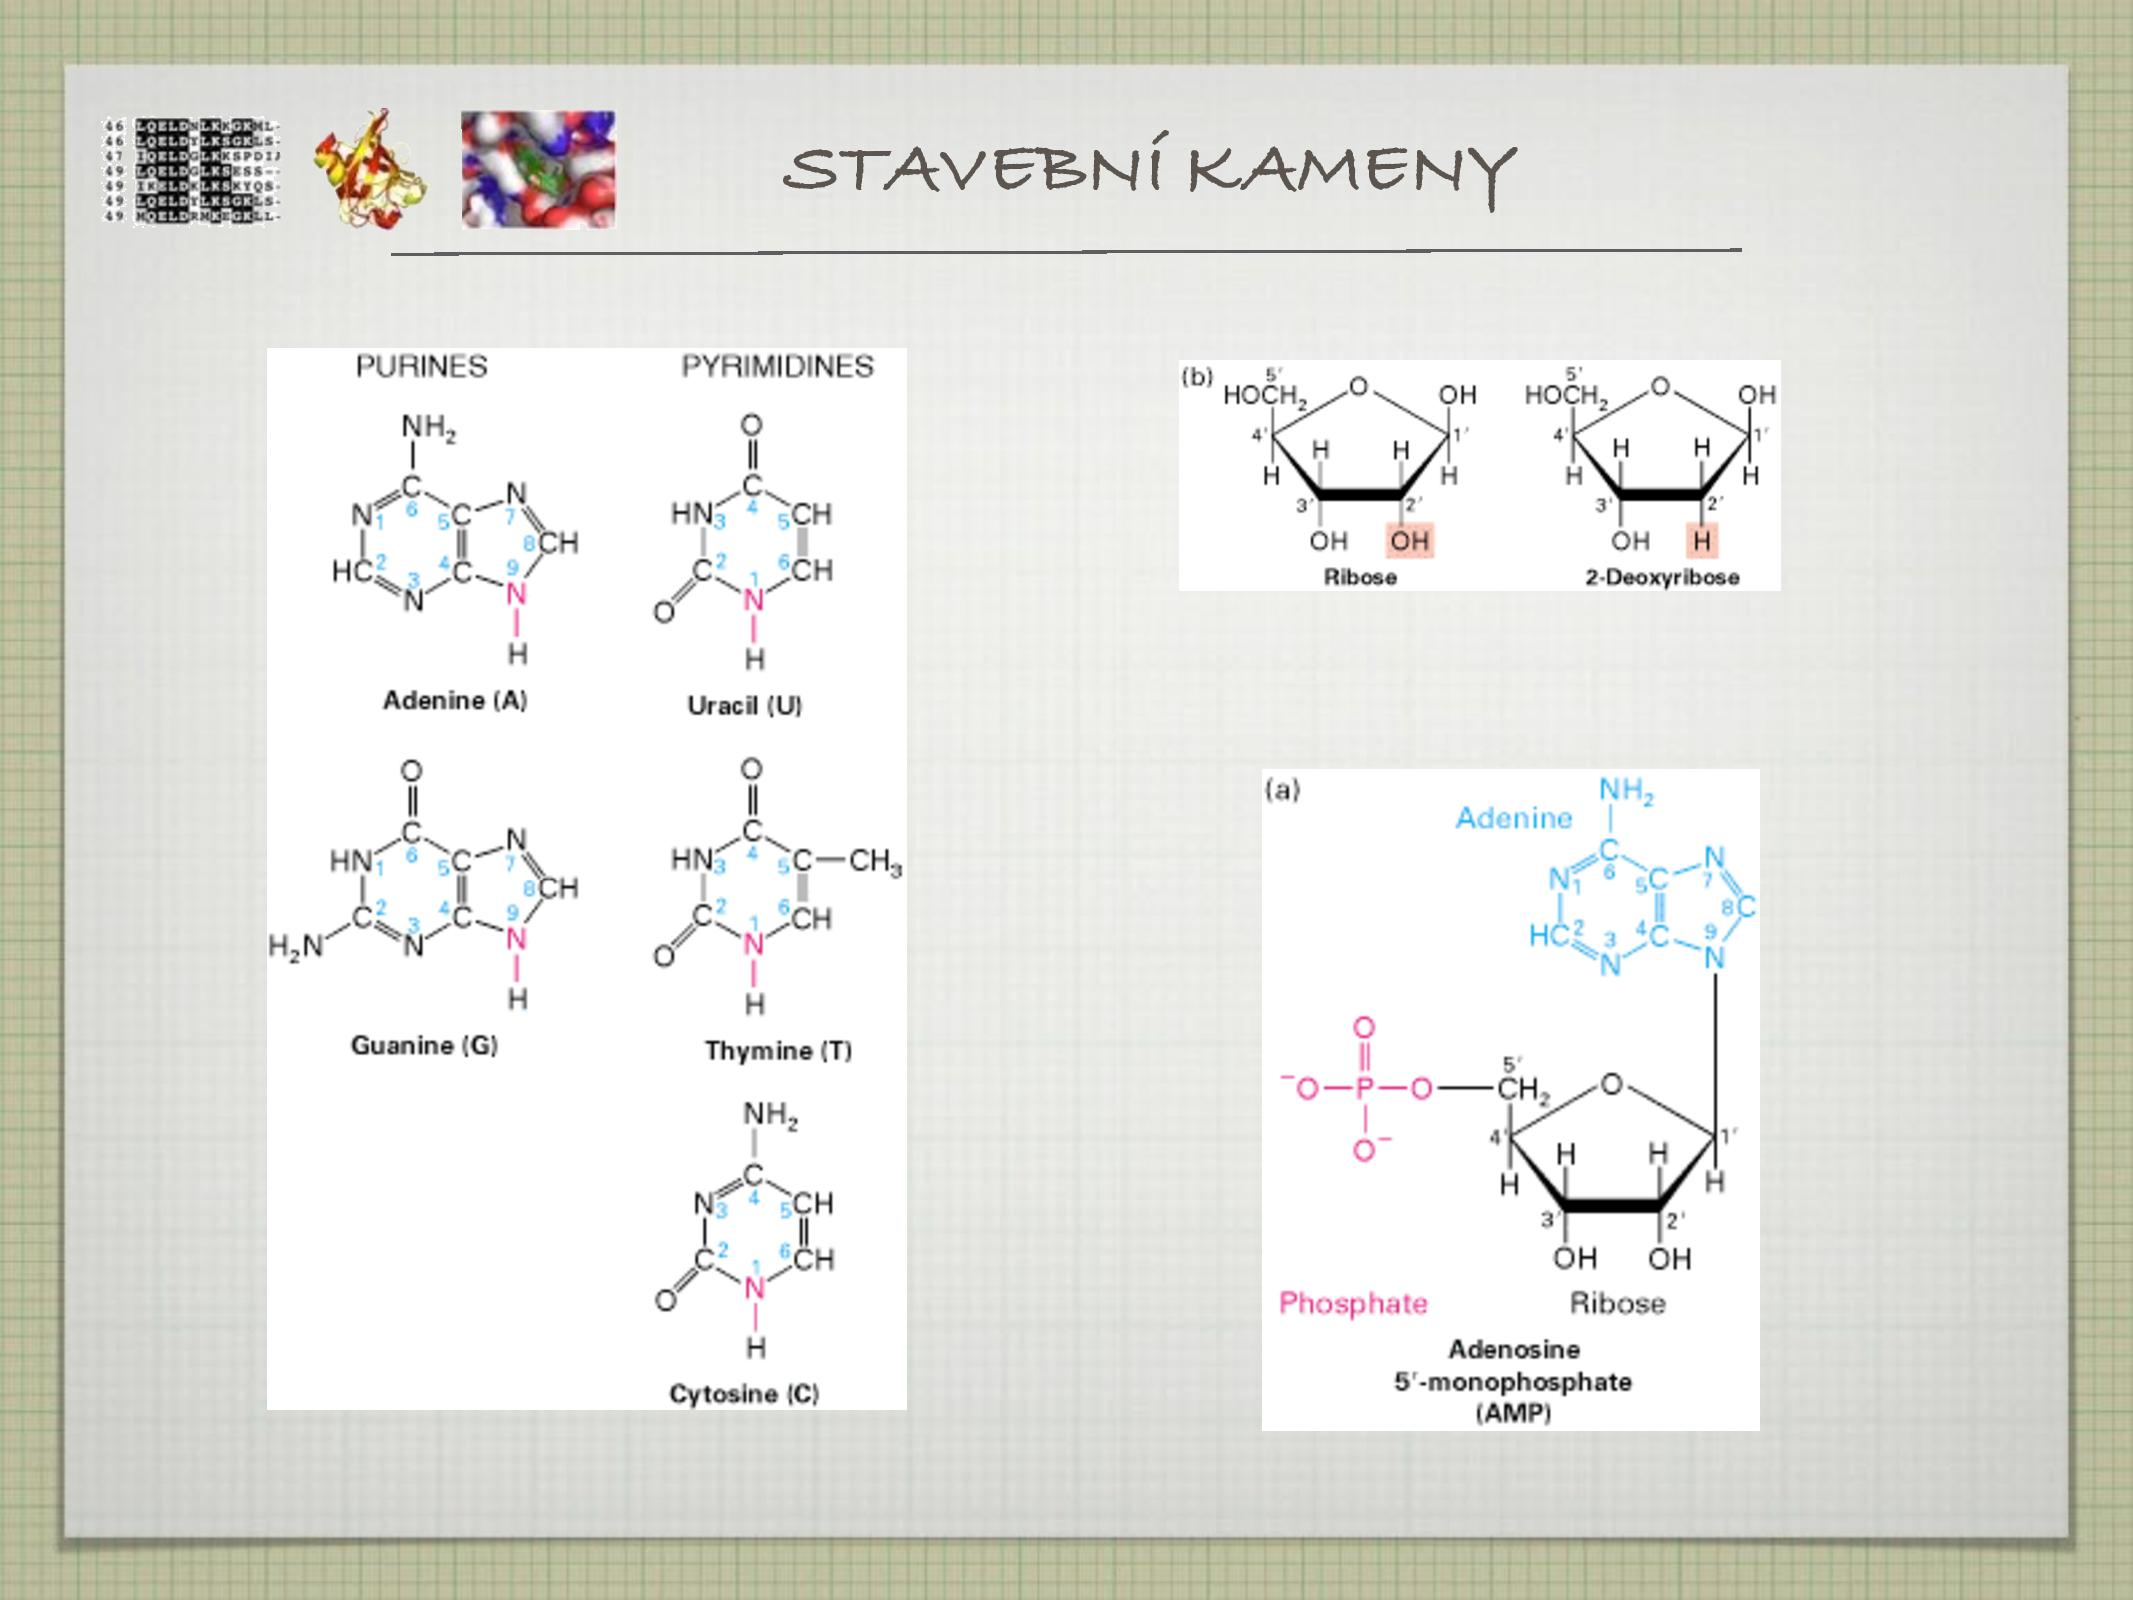
\includegraphics[width=0.85\textwidth]{slides-1/slide-10.jpg}
    \centering
    \label{slides-1-slide-10}
\end{figure}

\paragraph{Stavební kameny}
\begin{itemize}[nosep]
    \item puriny (adenosin, guanin), pyrymidiny (thyrosin, uracil, cytosin)
    \item ribosa, 2-deoxyribosa
    \item fosfát
\end{itemize}



\begin{figure}
    \caption{Prezentace č. 1, slide č. 11}
    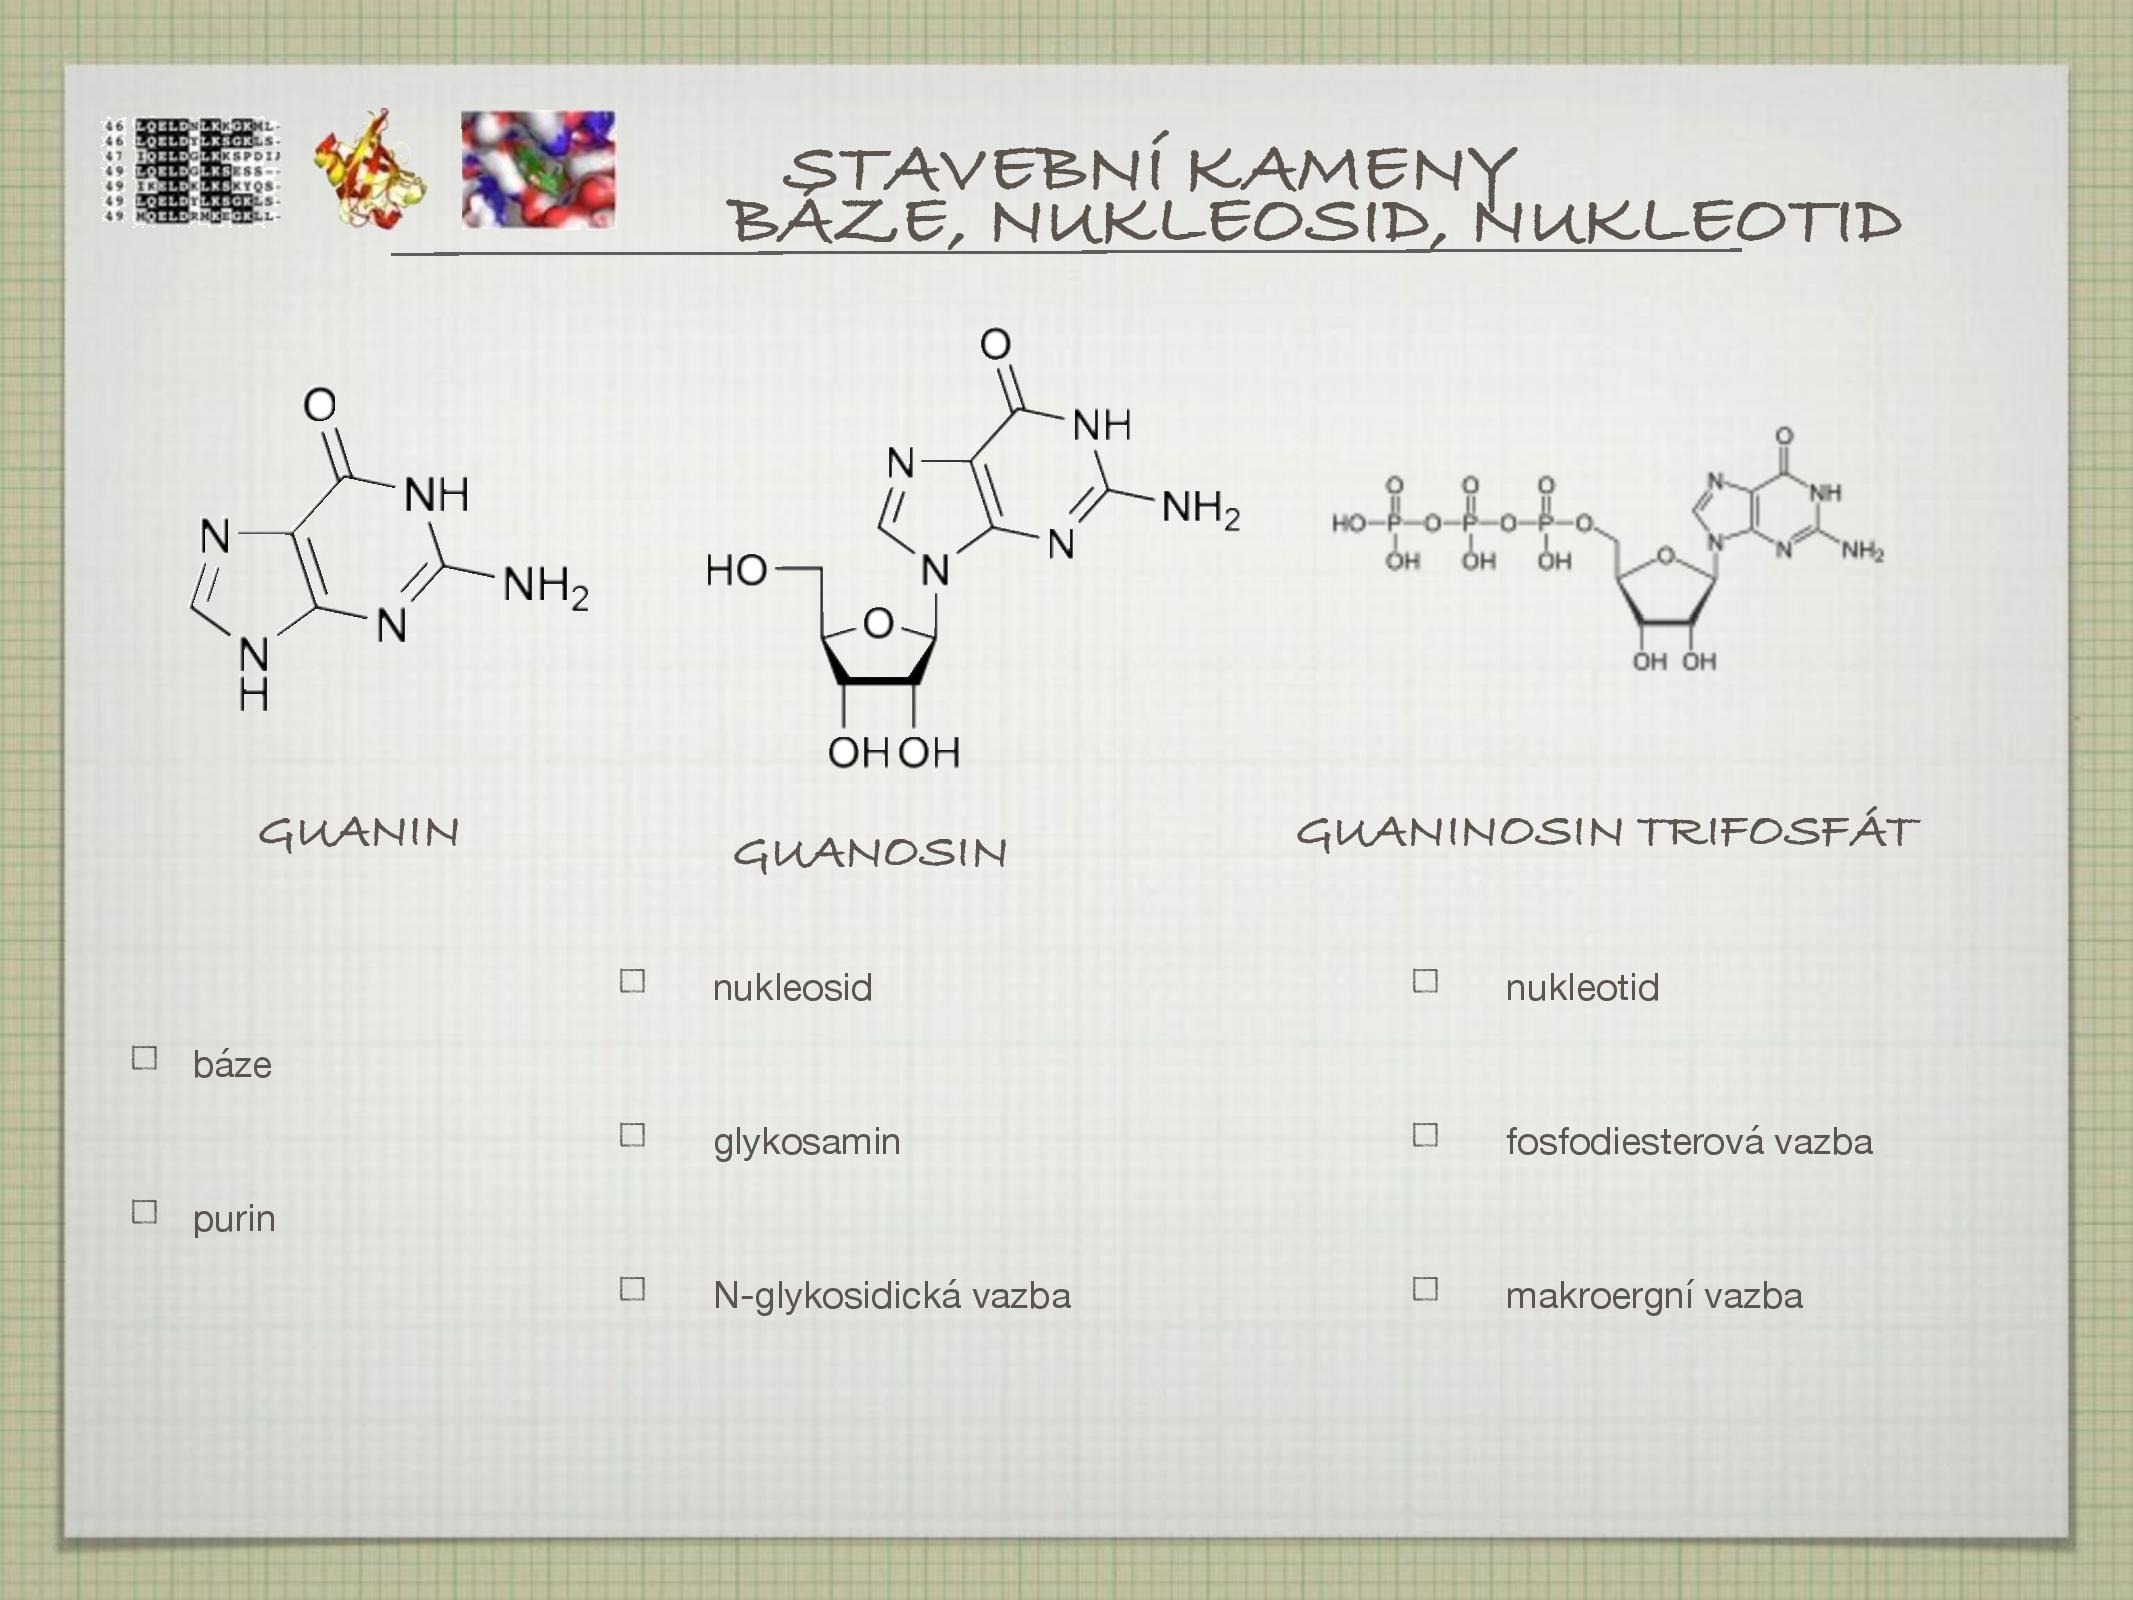
\includegraphics[width=0.85\textwidth]{slides-1/slide-11.jpg}
    \centering
    \label{slides-1-slide-11}
\end{figure}

\begin{description}
\item[guanin]\hfill \\
viz slide, běžná purinová báze


\item[guanosin]\hfill \\
nukleosid guaninu, tj. guanin + cukr vázaná N-glykosidickou vazbou


\item[guanosin trifosfát]\hfill \\
nukleotid guaninu, tj. guanosin + fosfát navázaný fosfodiesterovou vazbou

\end{description}


\begin{figure}
    \caption{Prezentace č. 1, slide č. 12}
    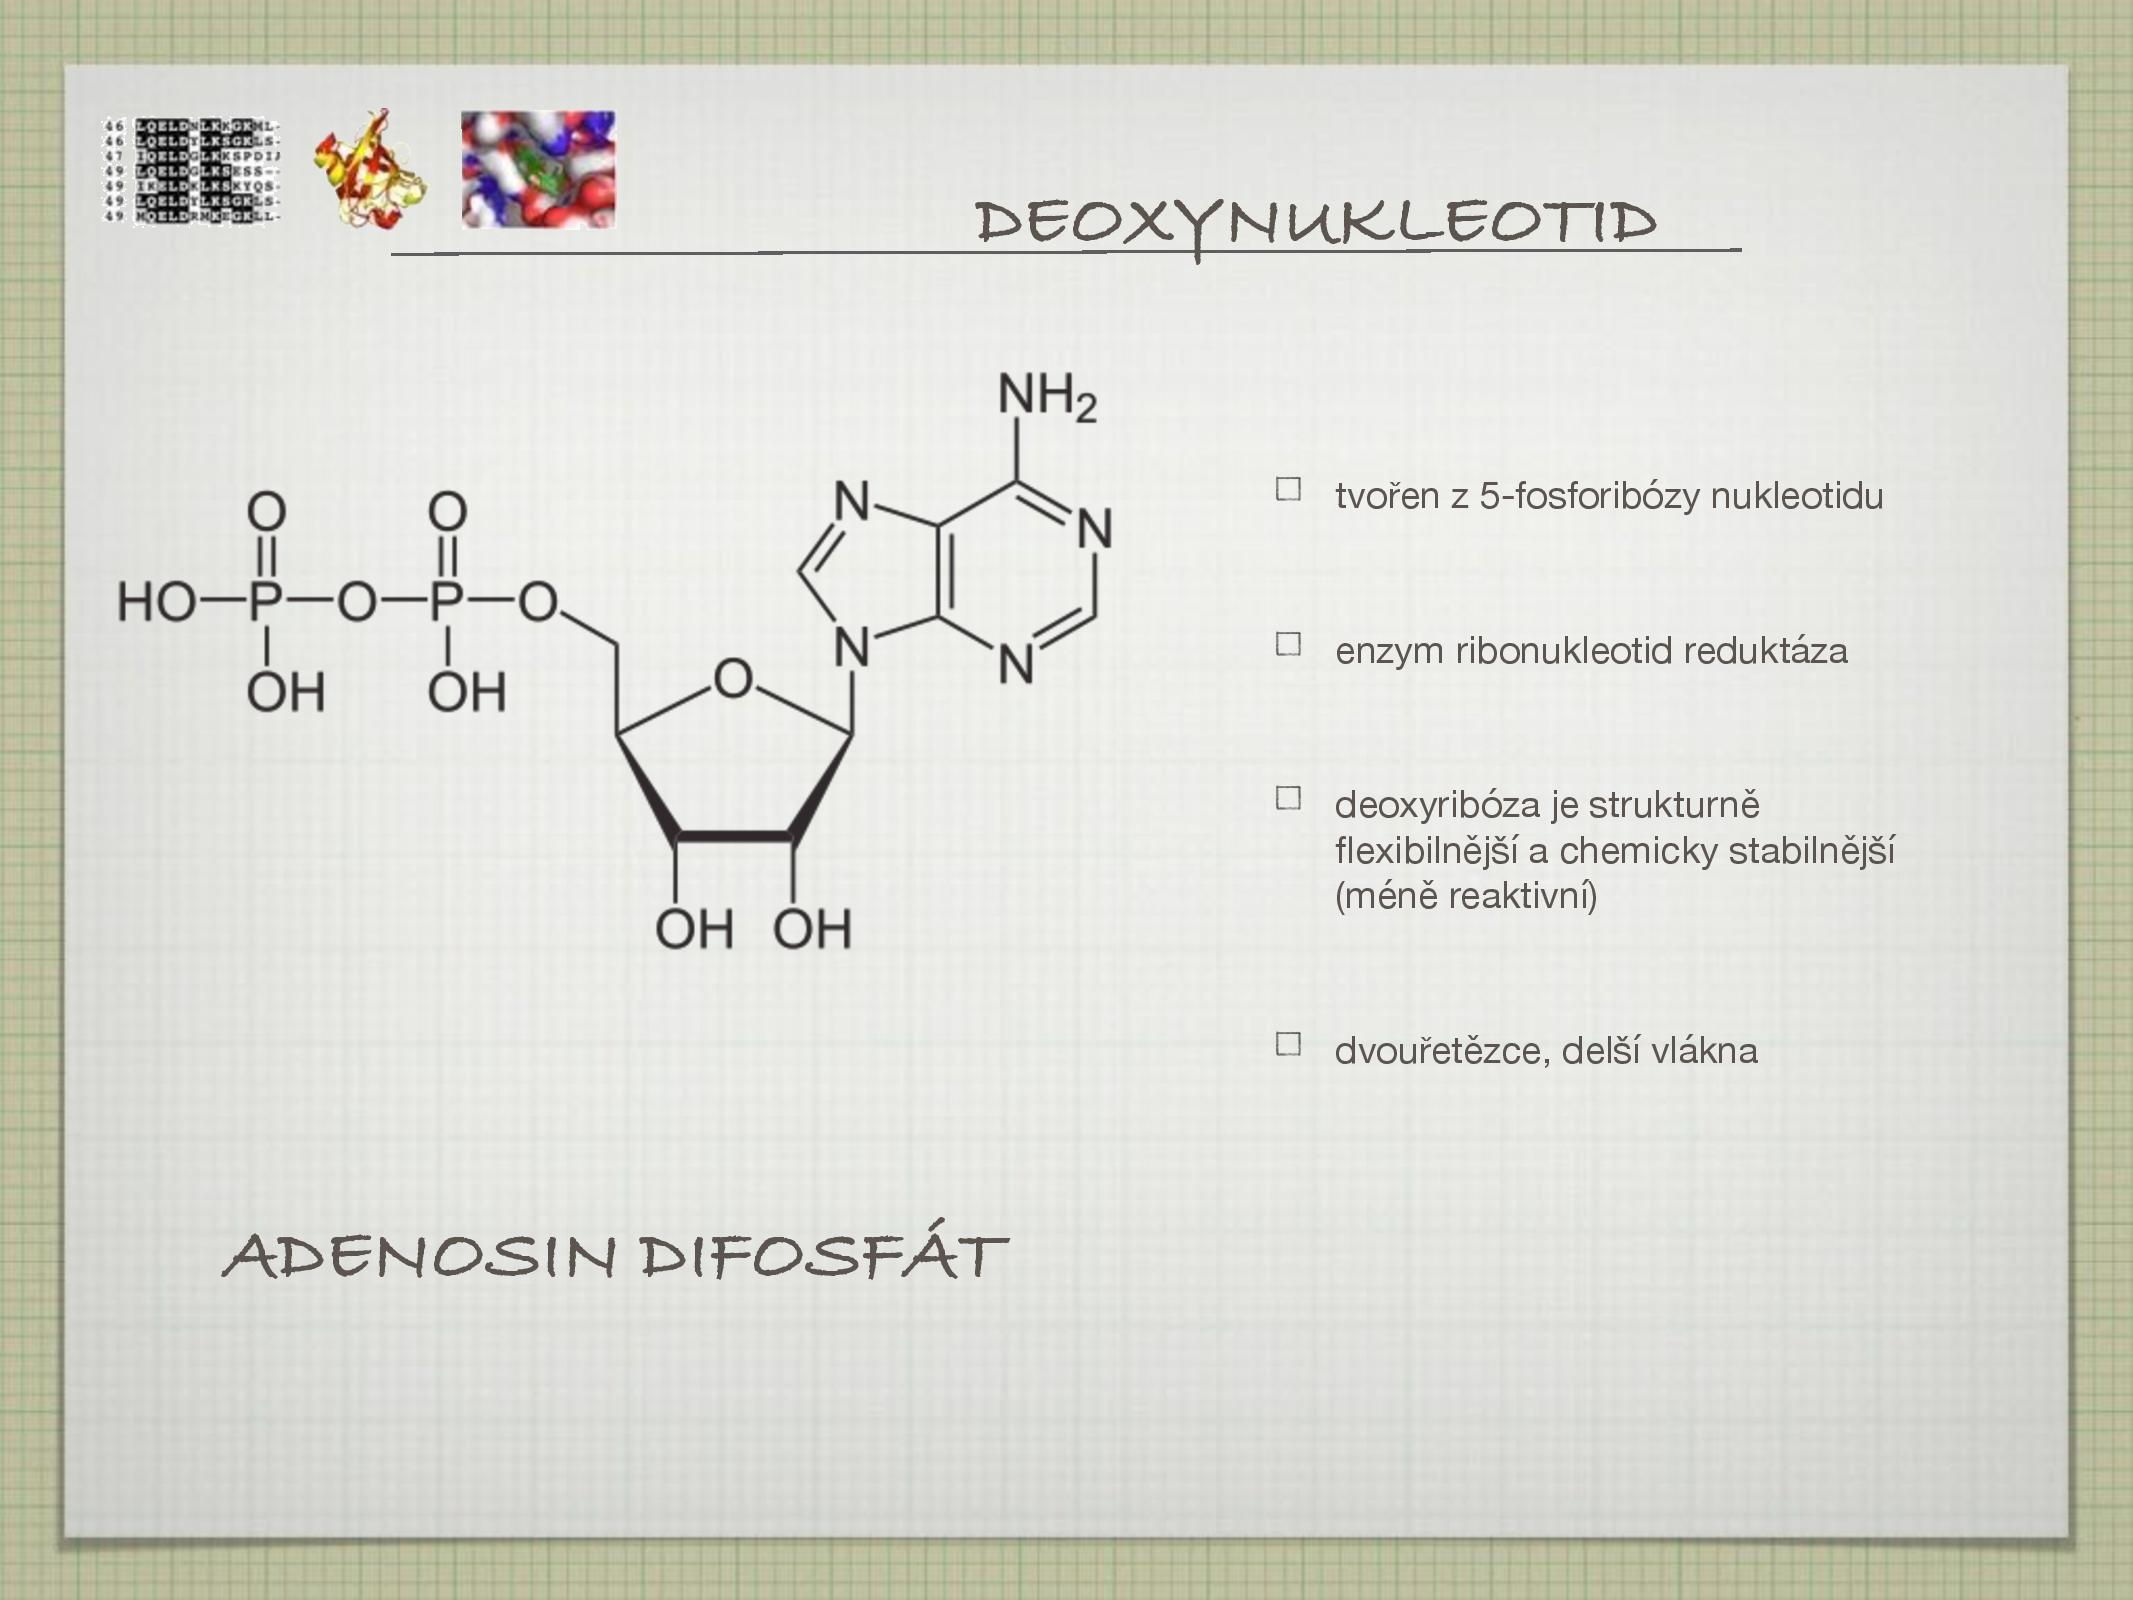
\includegraphics[width=0.85\textwidth]{slides-1/slide-12.jpg}
    \centering
    \label{slides-1-slide-12}
\end{figure}

\paragraph{Deoxynukleotid}
\begin{itemize}[nosep]
    \item na druhém uhlíku má cukr \(\ce{H}\) místo \(\ce{OH}\)
    \item vznik z nukleotidu redukovaného ribonukleotid reduktázou
    \item deoxyribóza je flexibilnější a chemicky stabilnější (výhoda pro DNA, které by se němělo měnit), protože \(\ce{OH}\) skupina je reaktivní
    \item stabilizace vede k tvoření delších vláken
\end{itemize}



\begin{figure}
    \caption{Prezentace č. 1, slide č. 13}
    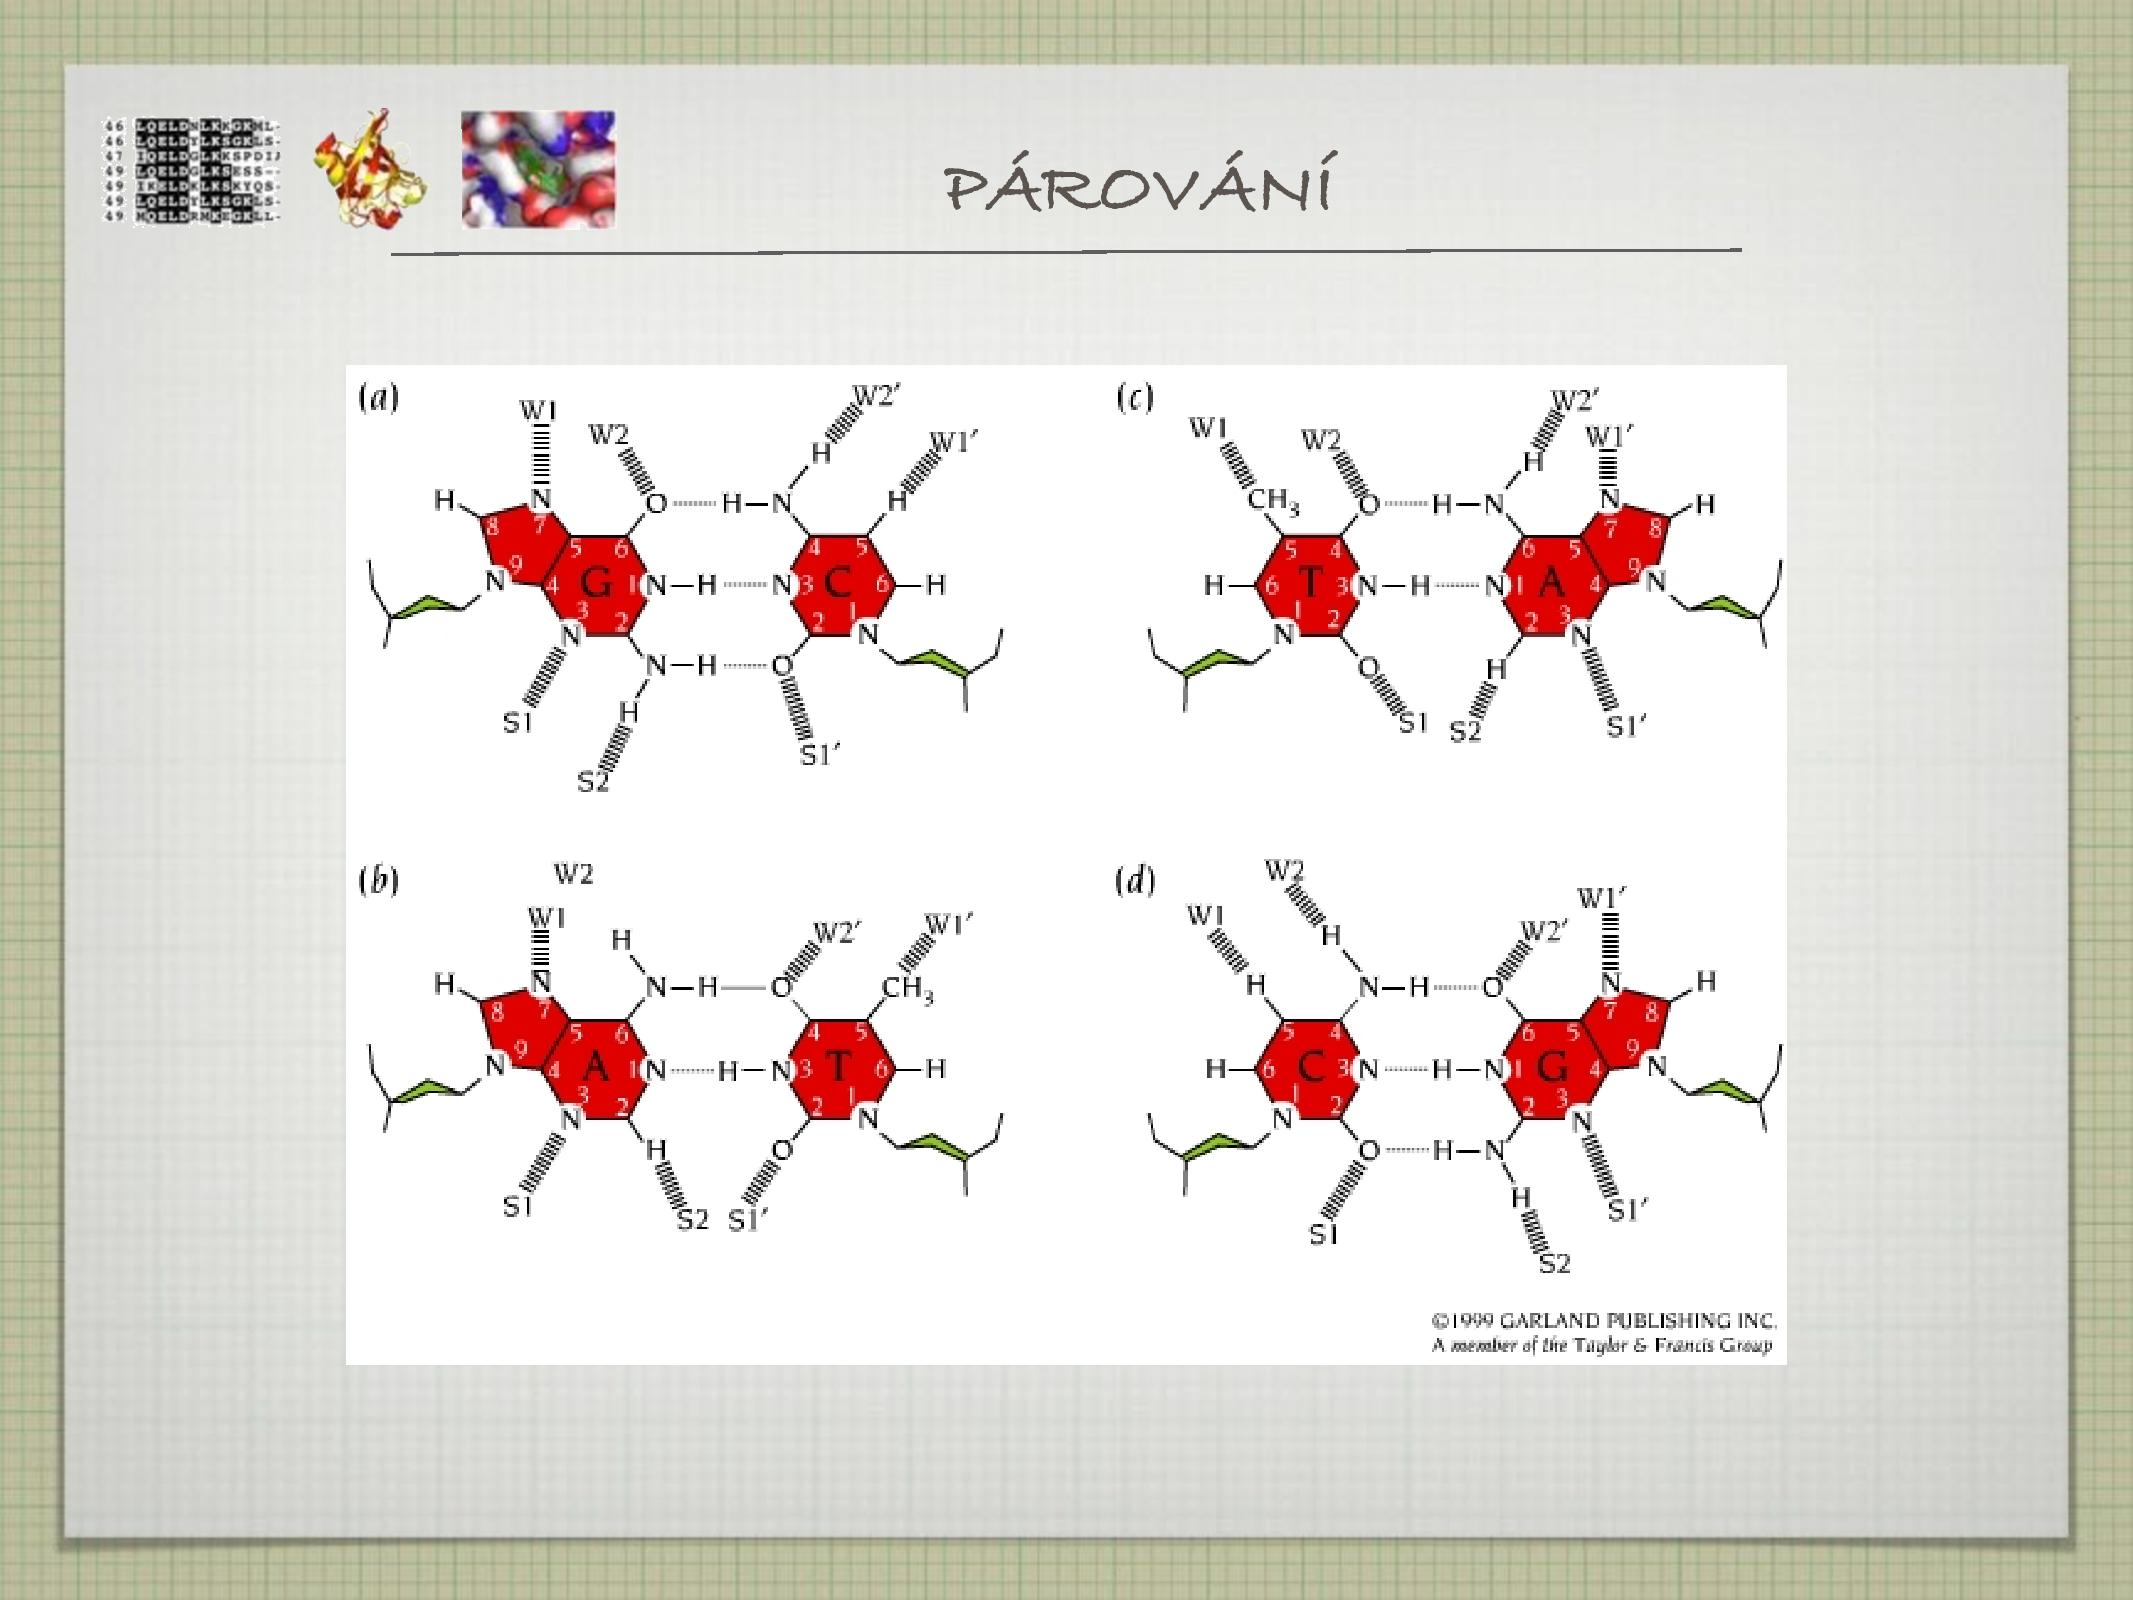
\includegraphics[width=0.85\textwidth]{slides-1/slide-13.jpg}
    \centering
    \label{slides-1-slide-13}
\end{figure}

\paragraph{Párování}
\begin{itemize}[nosep]
    \item díky něj vzniká sekundární struktura
    \item A + T páruje dvěma \(\ce{H}\) můstky, C + G třemi \(\ce{H}\) můstky
    \item AT bohaté úseky jsou tedy pružnější a GC úseky stabilnější
\end{itemize}



\paragraph{Vodíková vazba}
\begin{itemize}[nosep]
    \item nekovalentní přitažlivé interakce
    \item interakce dvou elektronegativních atomů, které jsou "spojeny" vodíkem
    \item vodík je připojen kovalentně k donoru a elektrostaticky k akceptoru (na vodíku vzniká parciální kladný náboj)
    \item délka 3Å
\end{itemize}



\begin{figure}
    \caption{Prezentace č. 1, slide č. 17}
    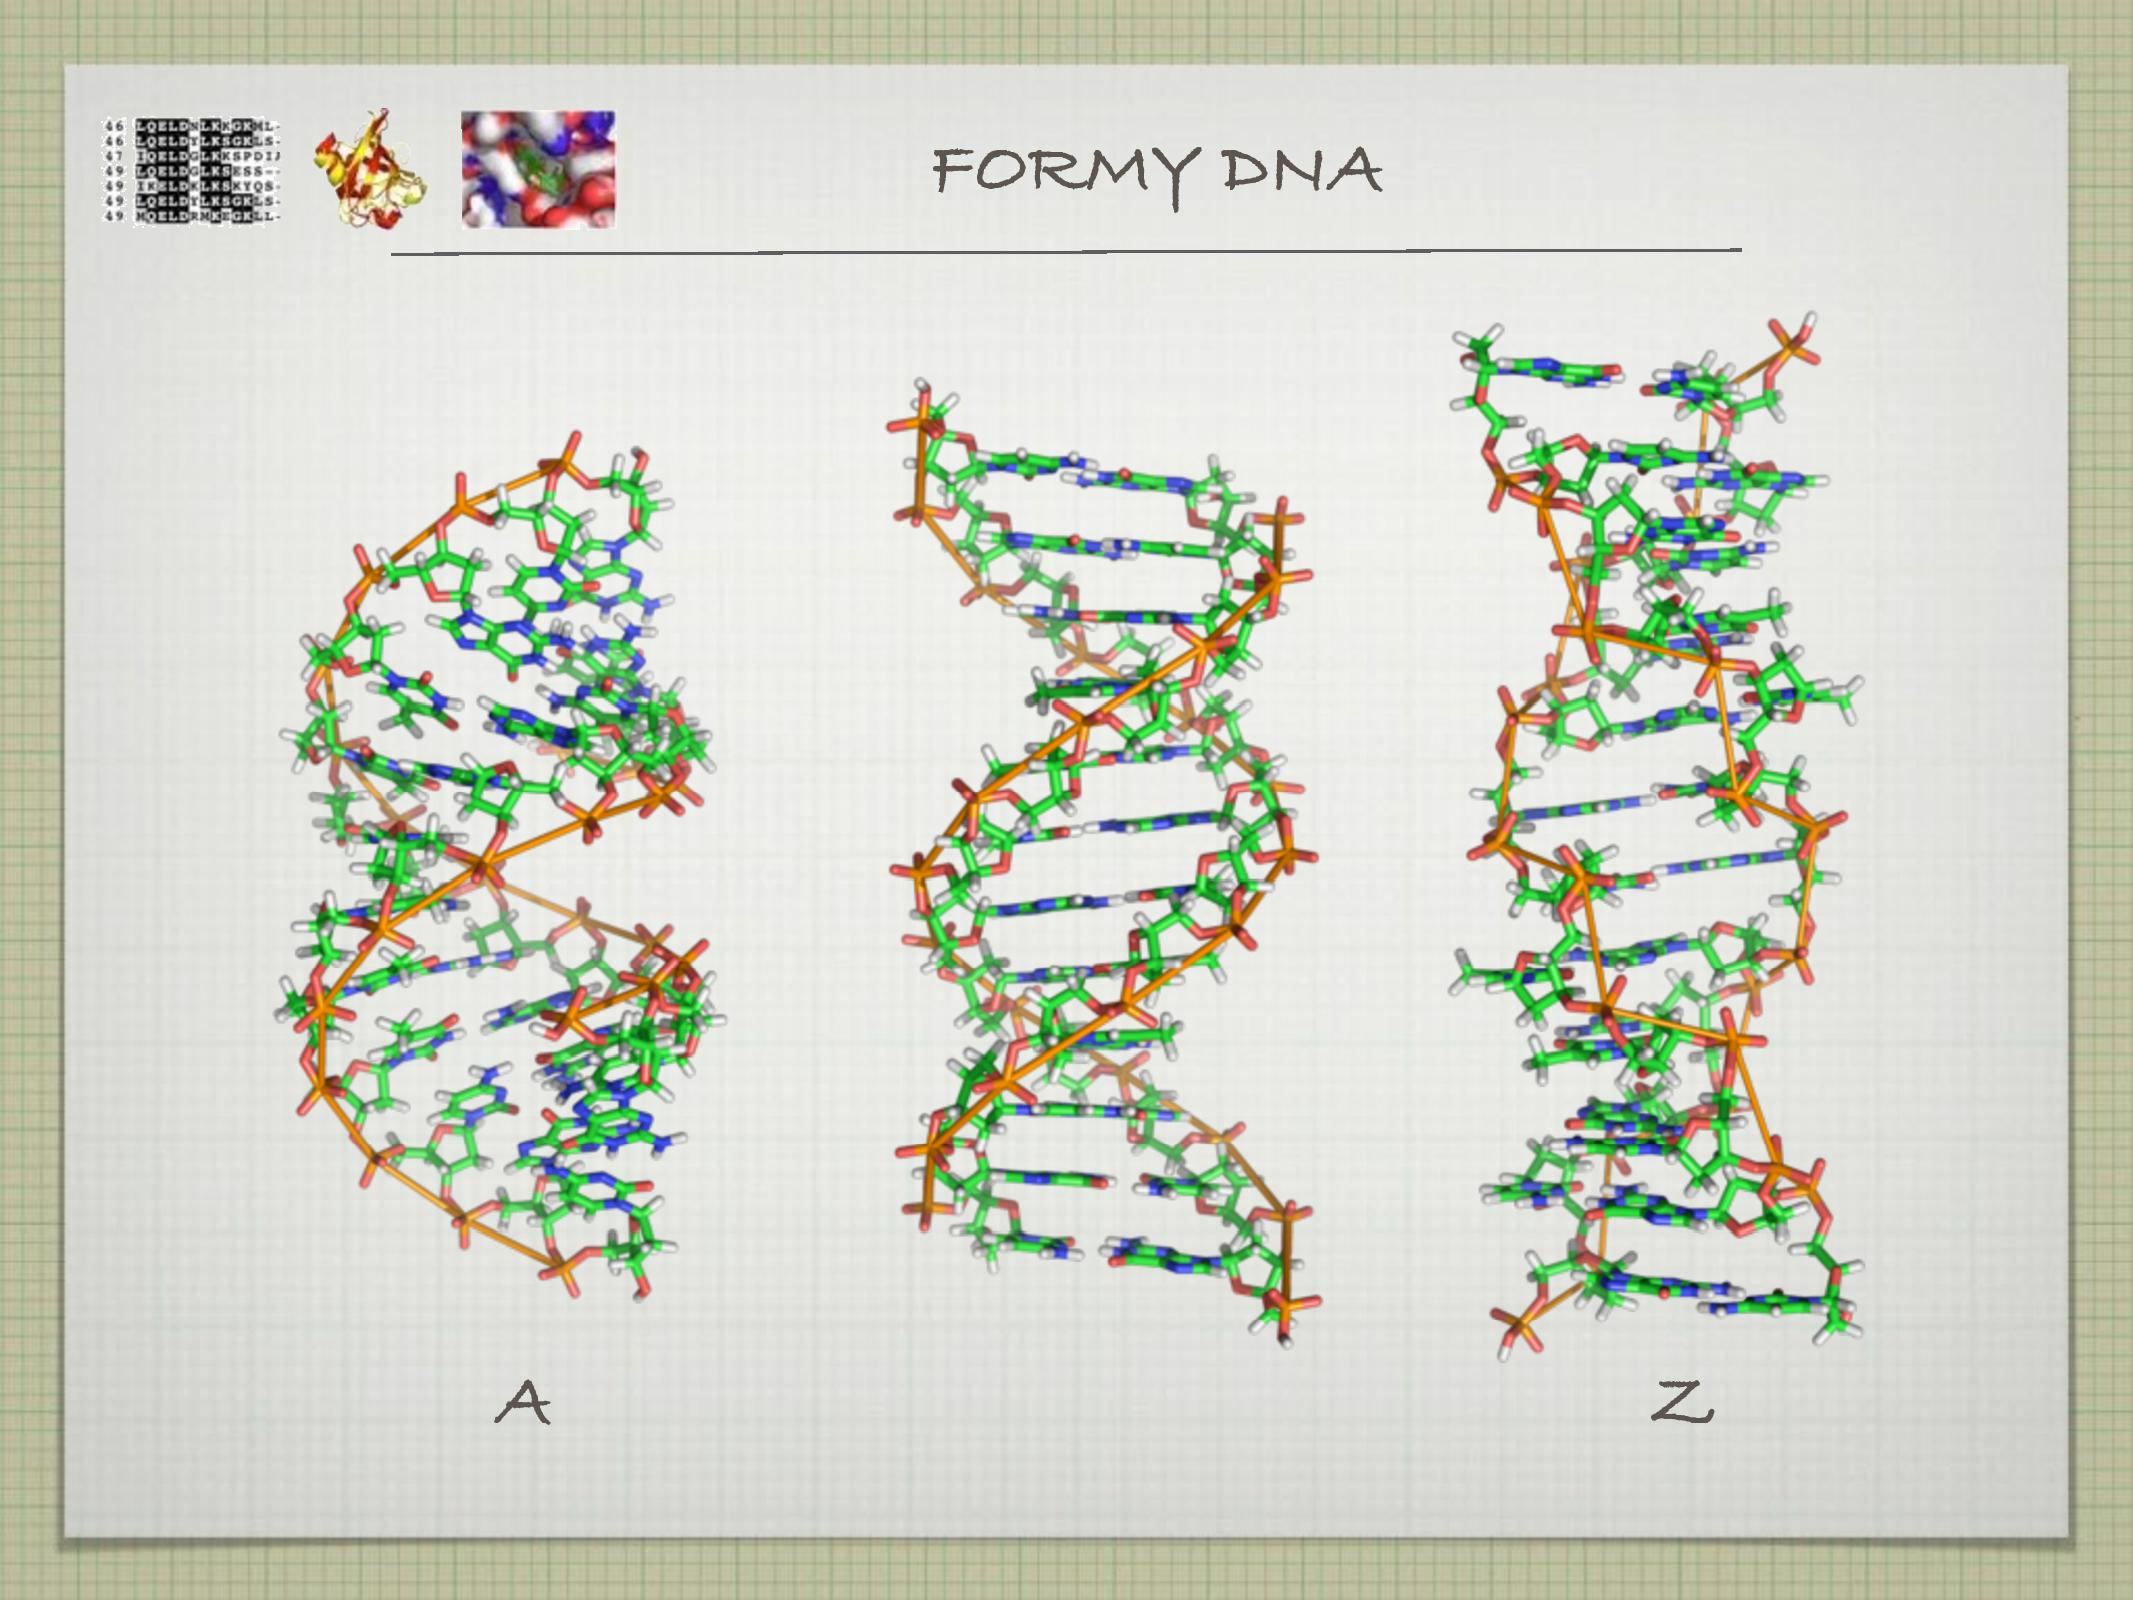
\includegraphics[width=0.85\textwidth]{slides-1/slide-17.jpg}
    \centering
    \label{slides-1-slide-17}
\end{figure}
\begin{figure}
    \caption{Prezentace č. 1, slide č. 18}
    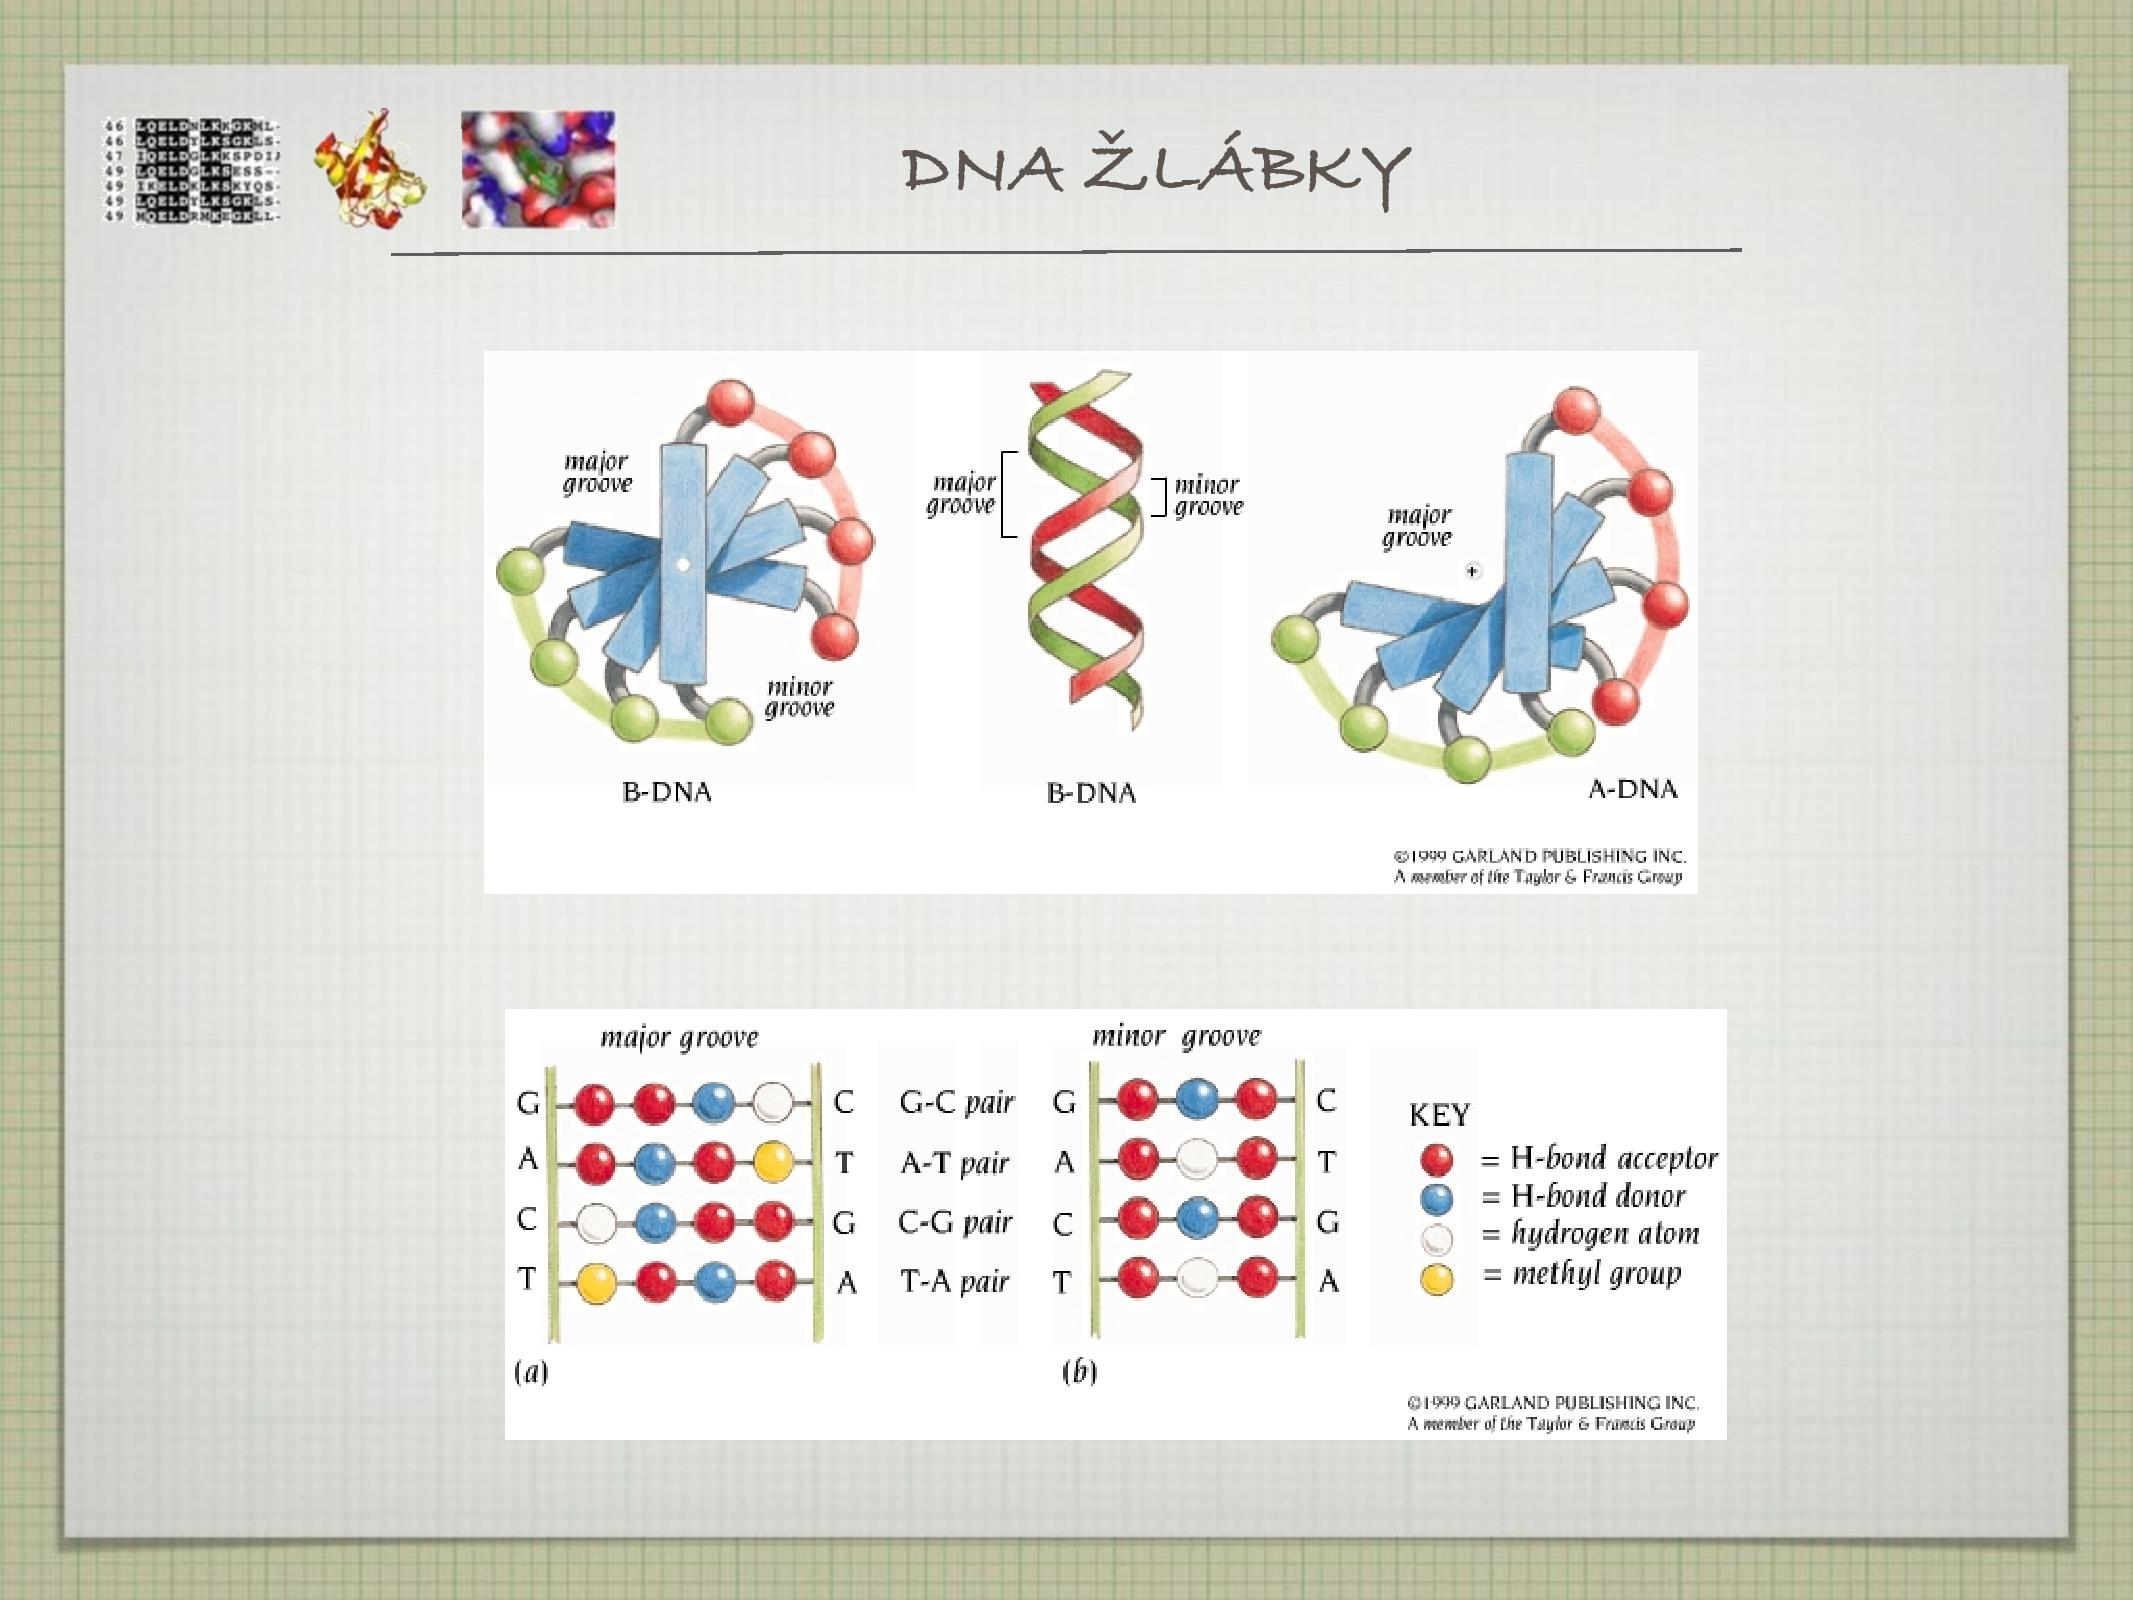
\includegraphics[width=0.85\textwidth]{slides-1/slide-18.jpg}
    \centering
    \label{slides-1-slide-18}
\end{figure}

\paragraph{Struktura DNA}
\begin{itemize}[nosep]
    \item dvoušroubovice (většinou pravotočivá)
    \item tři druhy: A, B, Z
\begin{itemize}[nosep]
    \item A má skoro stejně velké žlábky, mezeru uprostřed
    \item B je nejběžnější, má velký a malý žlábek
    \item Z není příliš častá, je levotočivá (na rozdíl od zbytku)
\end{itemize}

    \item žlábky hrají důležitou roli při vázání enzymů (přes žlábek lze vidět, jaké nukleotidy v DNA jsou)
\end{itemize}



\begin{figure}
    \caption{Prezentace č. 1, slide č. 19}
    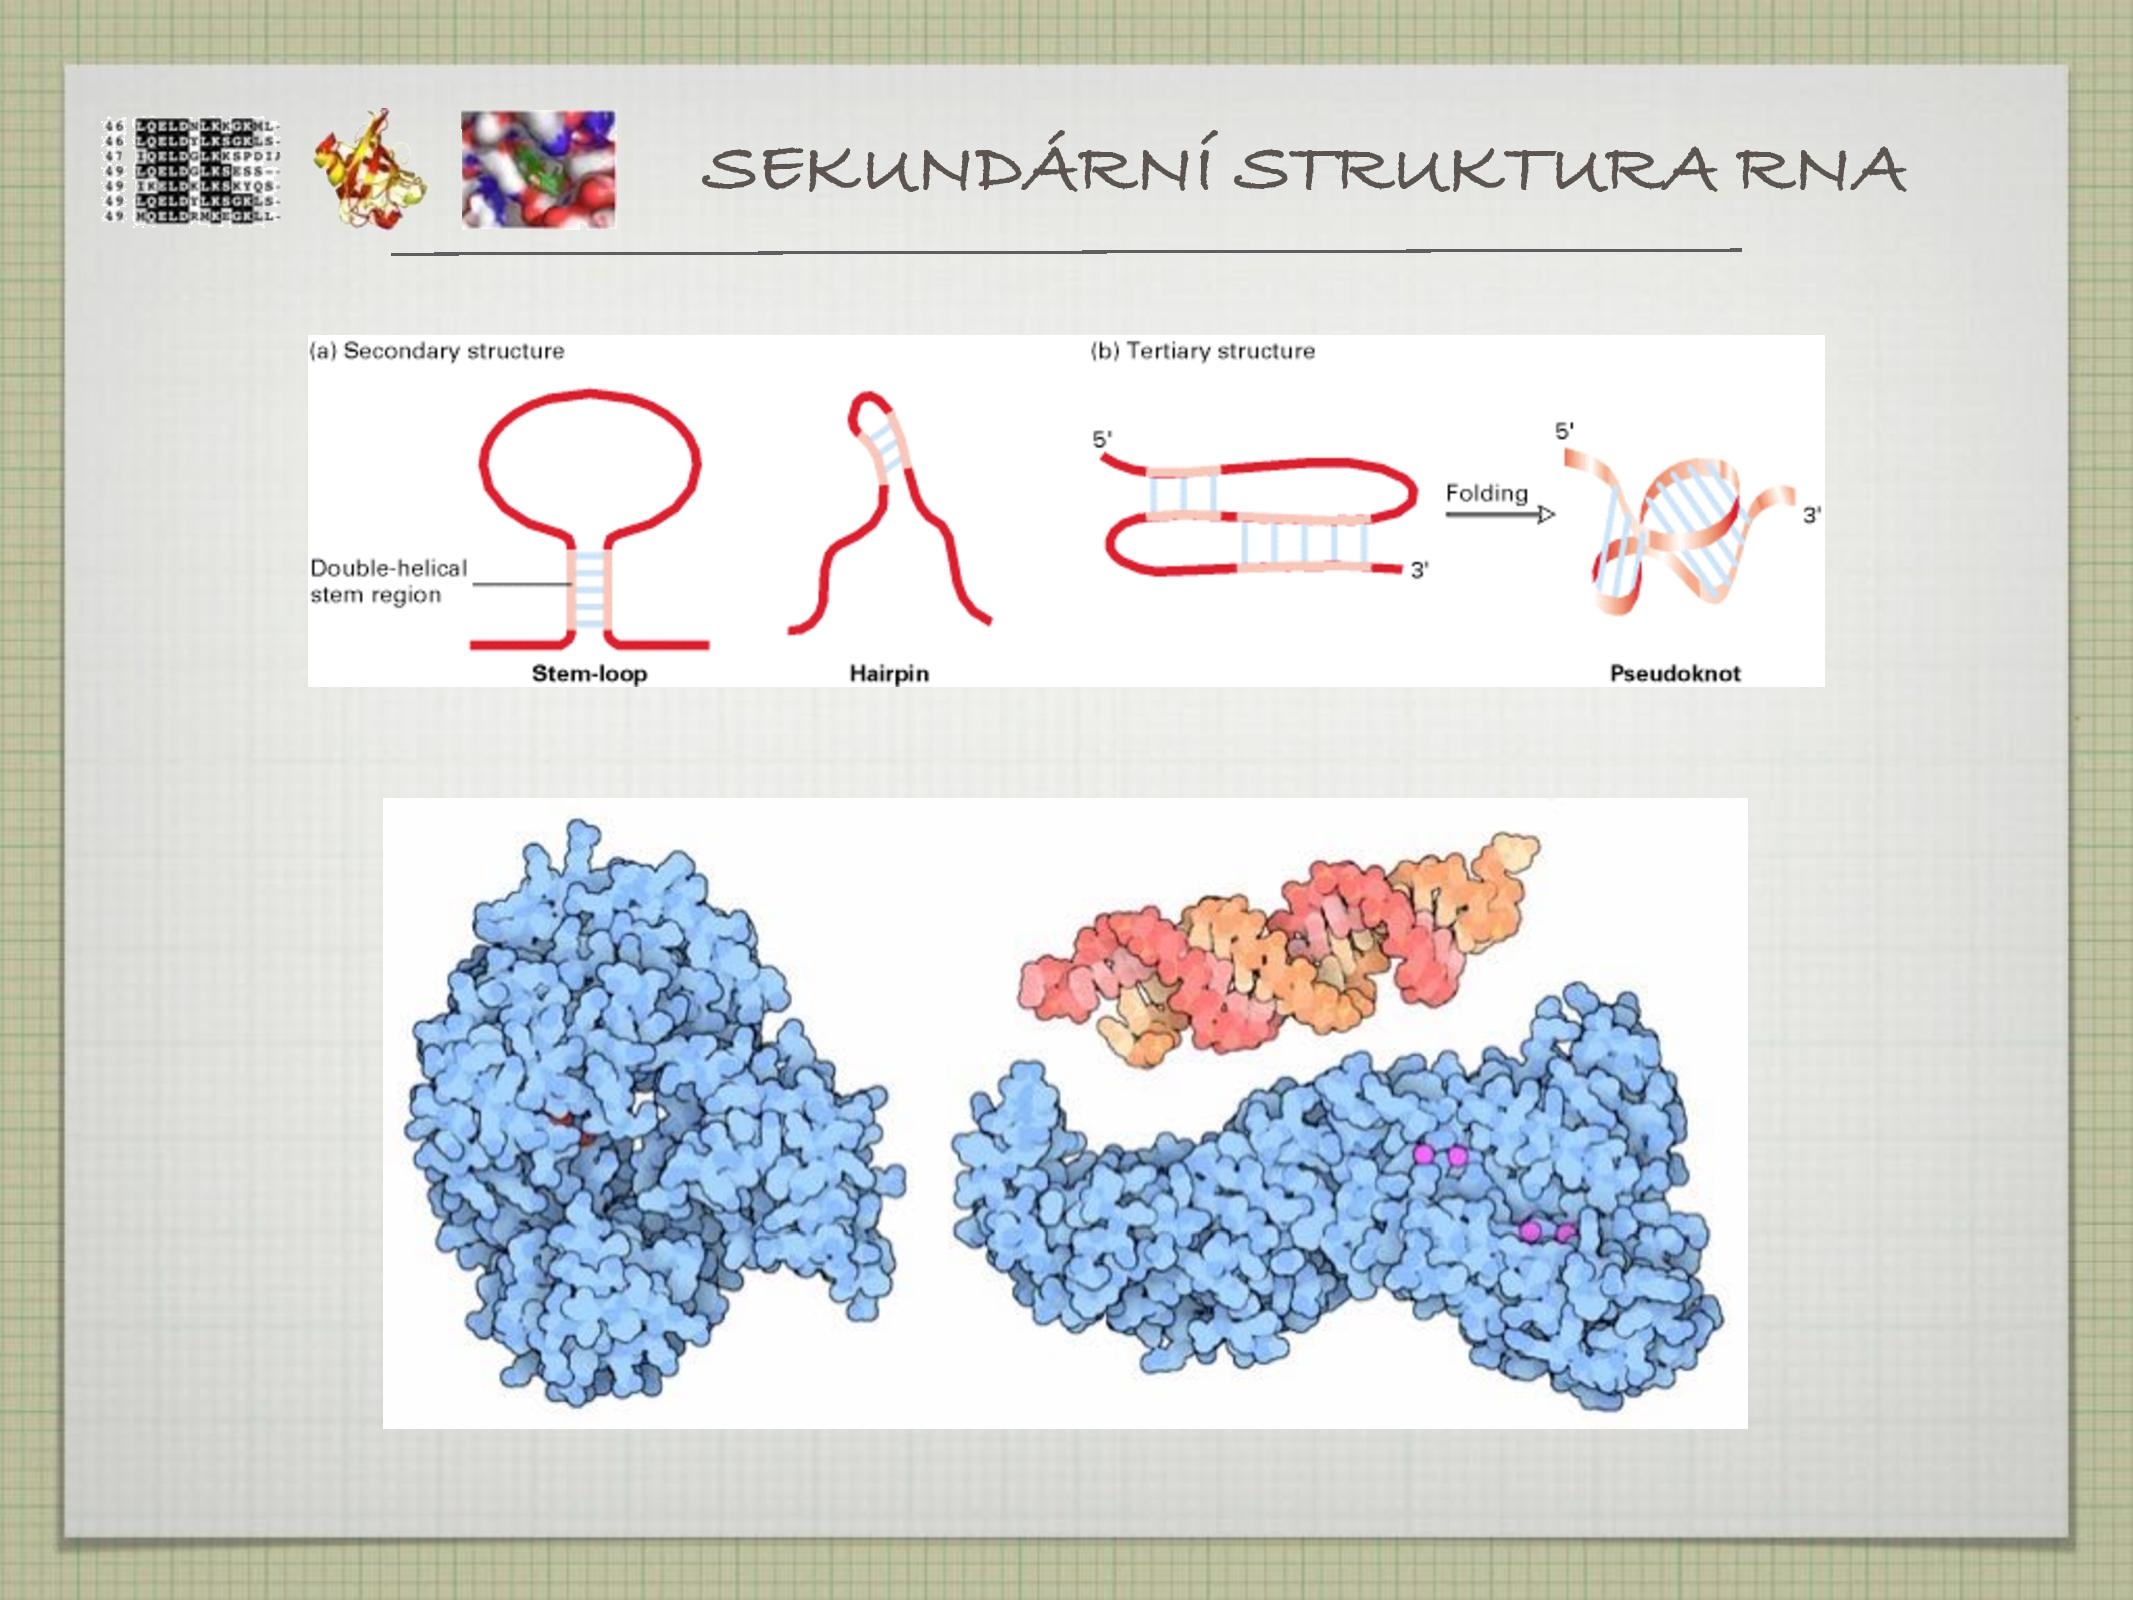
\includegraphics[width=0.85\textwidth]{slides-1/slide-19.jpg}
    \centering
    \label{slides-1-slide-19}
\end{figure}

\paragraph{Struktura RNA}
\begin{itemize}[nosep]
    \item loop, hairpin, pseudoknot
    \item většinou je tvořena pouze jedním vláknem
\end{itemize}




\chapter{Struktura proteinů} \label{Struktura proteinů}

\marginline{Přednáška č. 3}

\begin{figure}
    \caption{Prezentace č. 1, slide č. 21}
    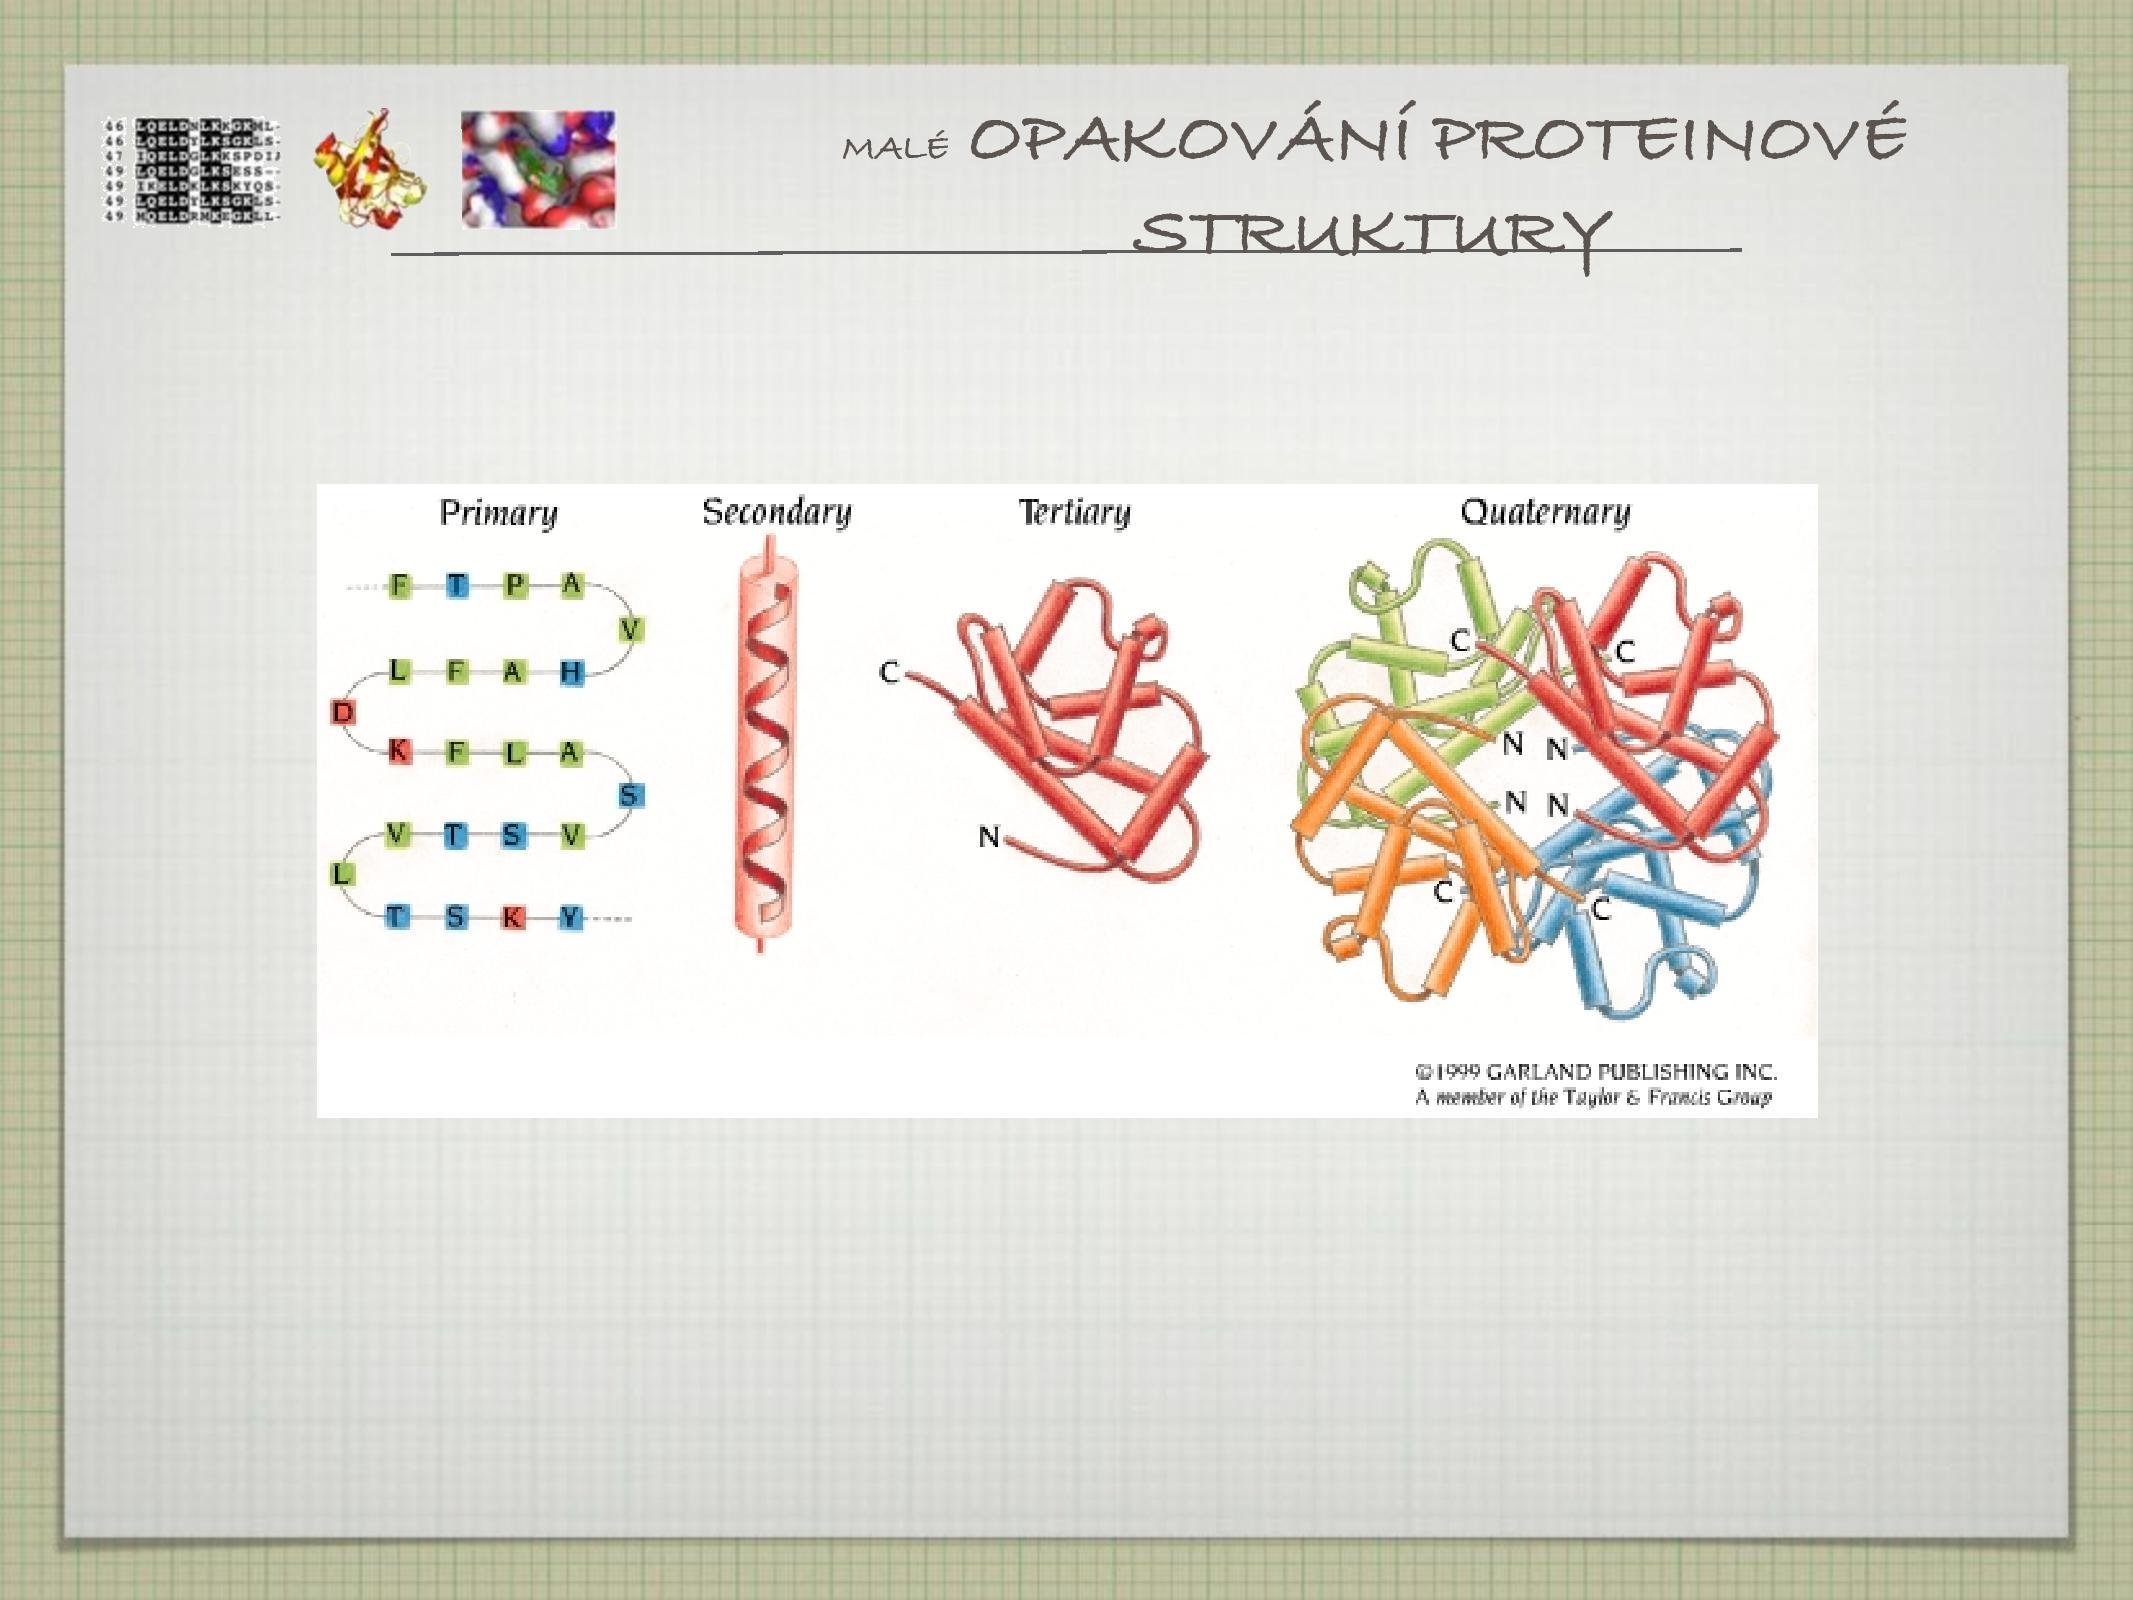
\includegraphics[width=0.85\textwidth]{slides-1/slide-21.jpg}
    \centering
    \label{slides-1-slide-21}
\end{figure}

Primární až kvartnerní; struktura určuje funkci proteinu (proto nás zajímá), například s čím reaguje, jakými membránami projde a za jakých podmínek atp.

\mybox{TODO}{Doplnit linky na zápisky z biopolymerů (až zde budou k dispozici).}


\section{Primární struktura} \label{Primární struktura}


Primární struktura je určená pořadím aminokyselin (AK). AK je 20+2.

\begin{figure}
    \caption{Prezentace č. 1, slide č. 22}
    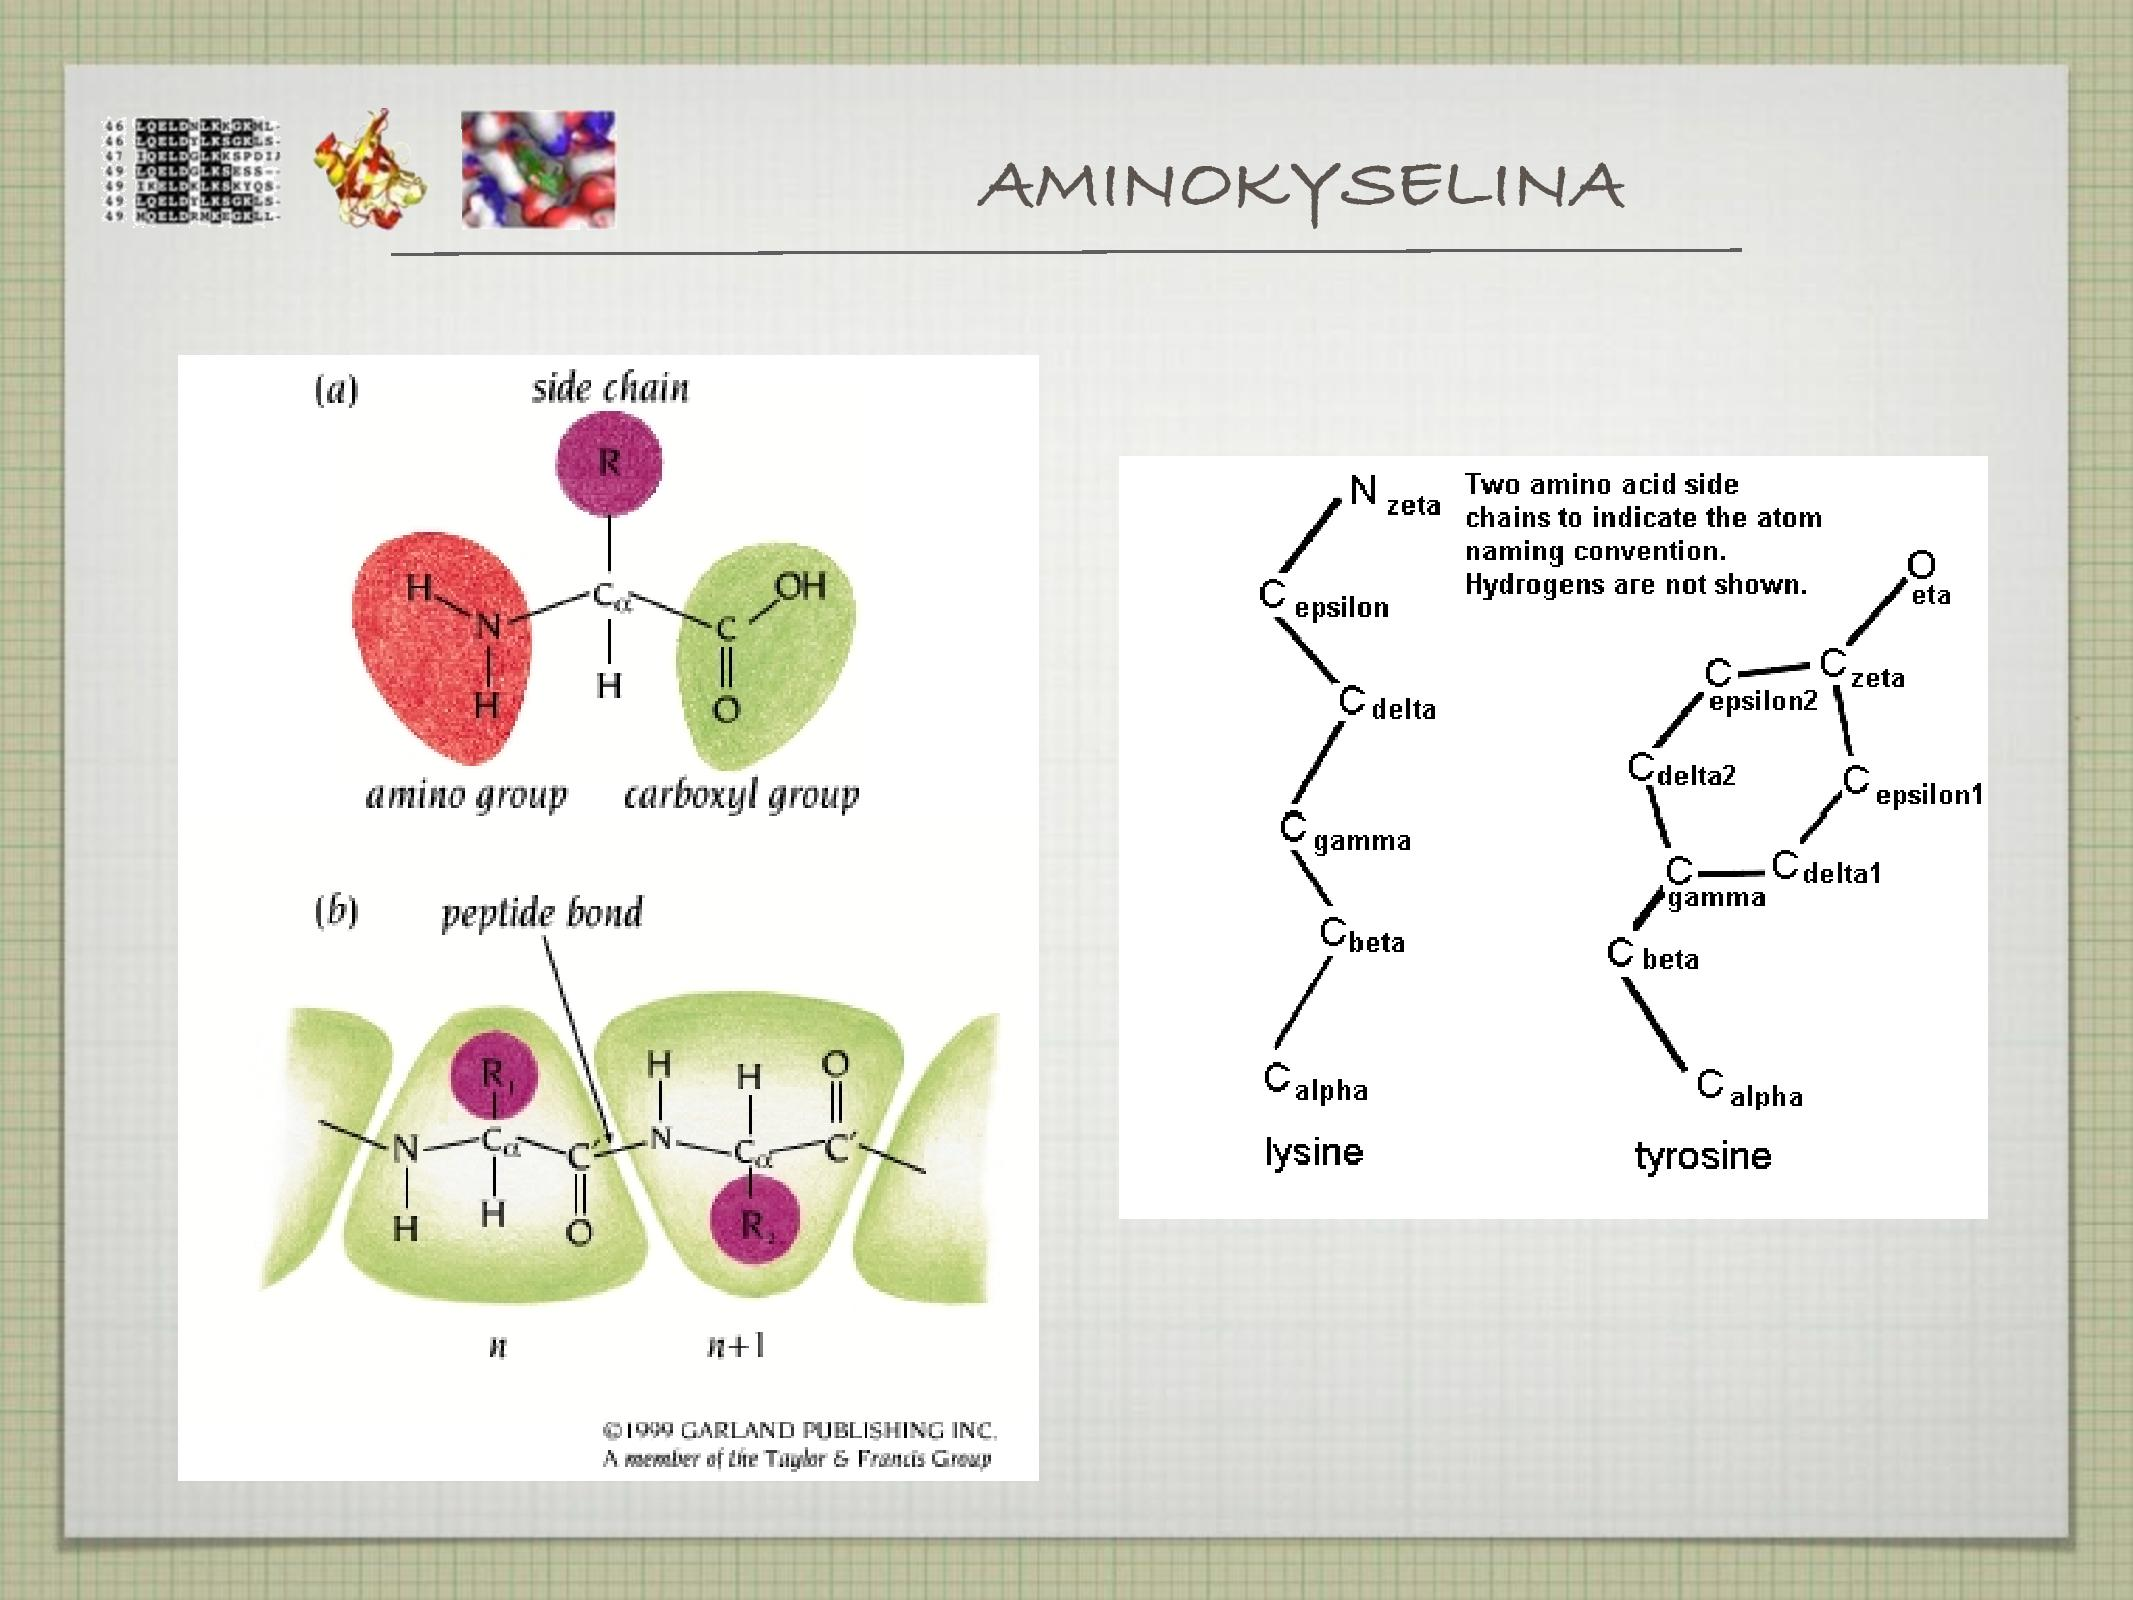
\includegraphics[width=0.85\textwidth]{slides-1/slide-22.jpg}
    \centering
    \label{slides-1-slide-22}
\end{figure}
\begin{figure}
    \caption{Prezentace č. 1, slide č. 51}
    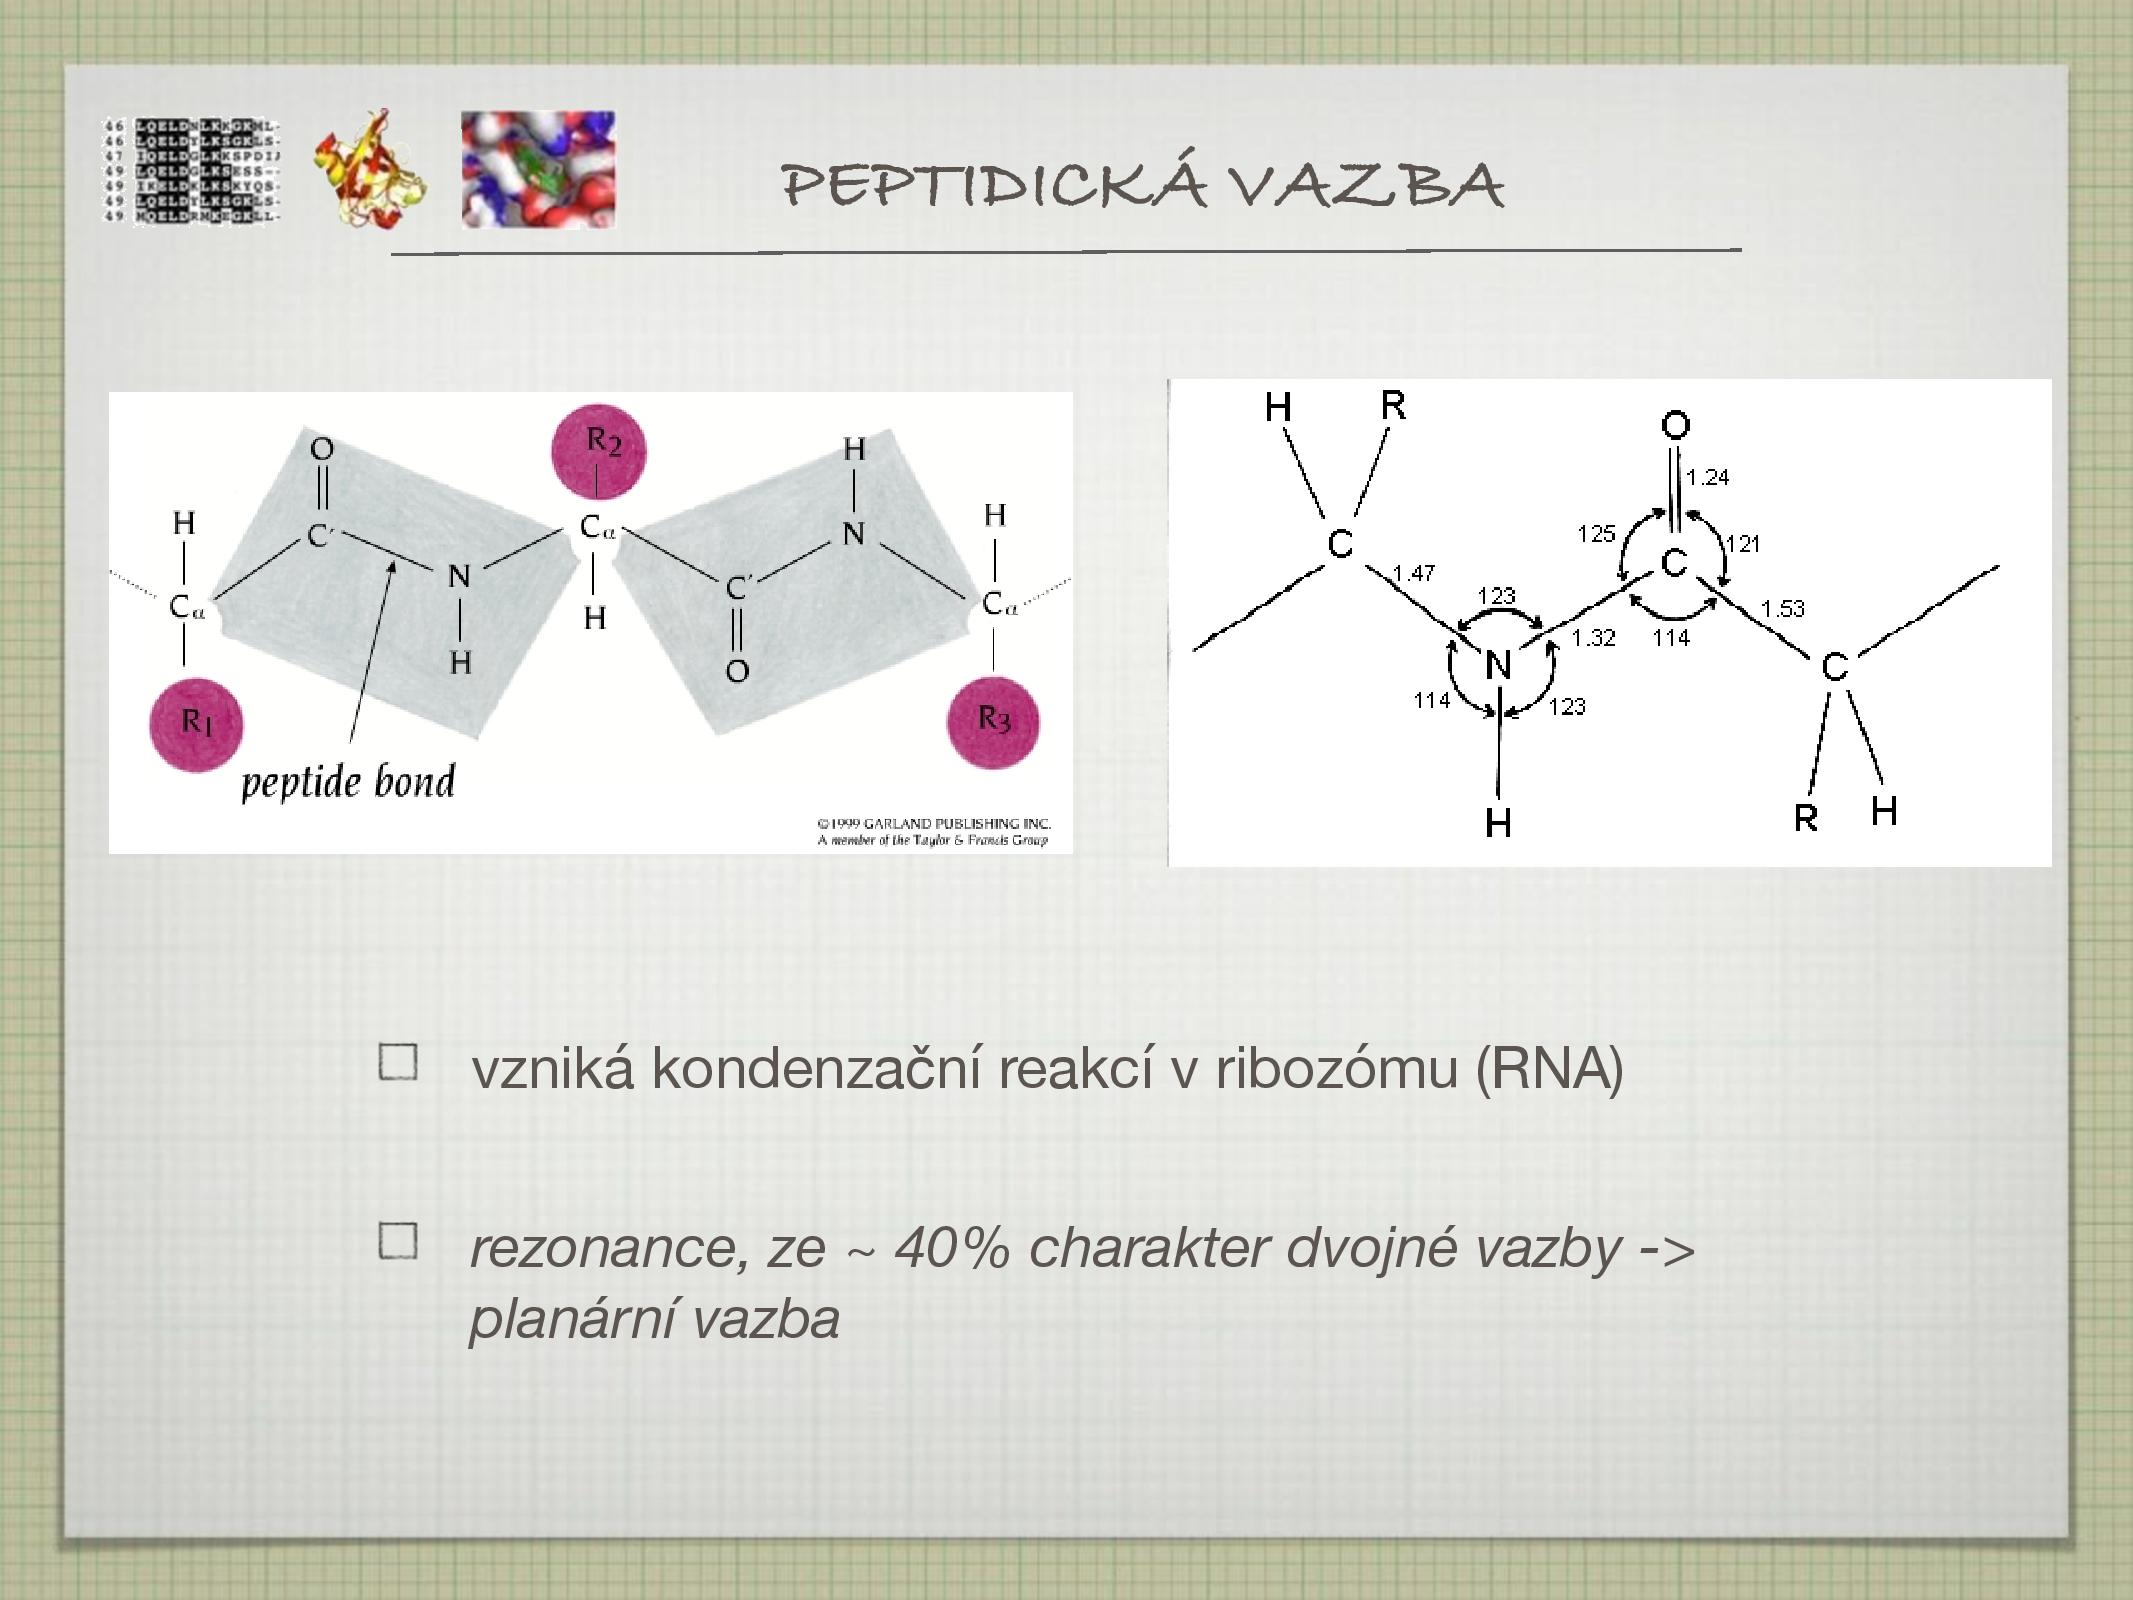
\includegraphics[width=0.85\textwidth]{slides-1/slide-51.jpg}
    \centering
    \label{slides-1-slide-51}
\end{figure}

\paragraph{Struktura AK}
\begin{itemize}[nosep]
    \item \(\ce{C_\alpha}\) je chirální, jsou na něm navázány čtyři různé skupiny
    \item \(\ce{NH2}\) se váže na \(\ce{COOH}\) za vzniku peptidické vazby, uvolňuje se \(\ce{H2O}\)
\begin{itemize}[nosep]
    \item peptidická vazba je planární, vzniká pomyslný čtyřúhelník s rohy v \(\ce{C_\alpha}\)
    \item ze 40\% má charakter dvojné vazby
\begin{itemize}[nosep]
    \item je kratší než jednoduchá
    \item je planární
    \item má cis a trans kofiguraci
\end{itemize}

    \item rotace je tedy možná pouze v \(\ce{C_\alpha}\), existují dva torzní úhly (\(\phi, \psi\))
\begin{itemize}[nosep]
    \item teoreticky možné a prakticky spočítané hodnoty torzních úhlů se zaznamenávají do \emph{Ramachandranova diagramu}
\end{itemize}

\end{itemize}

\end{itemize}



\begin{figure}
    \caption{Prezentace č. 1, slide č. 23}
    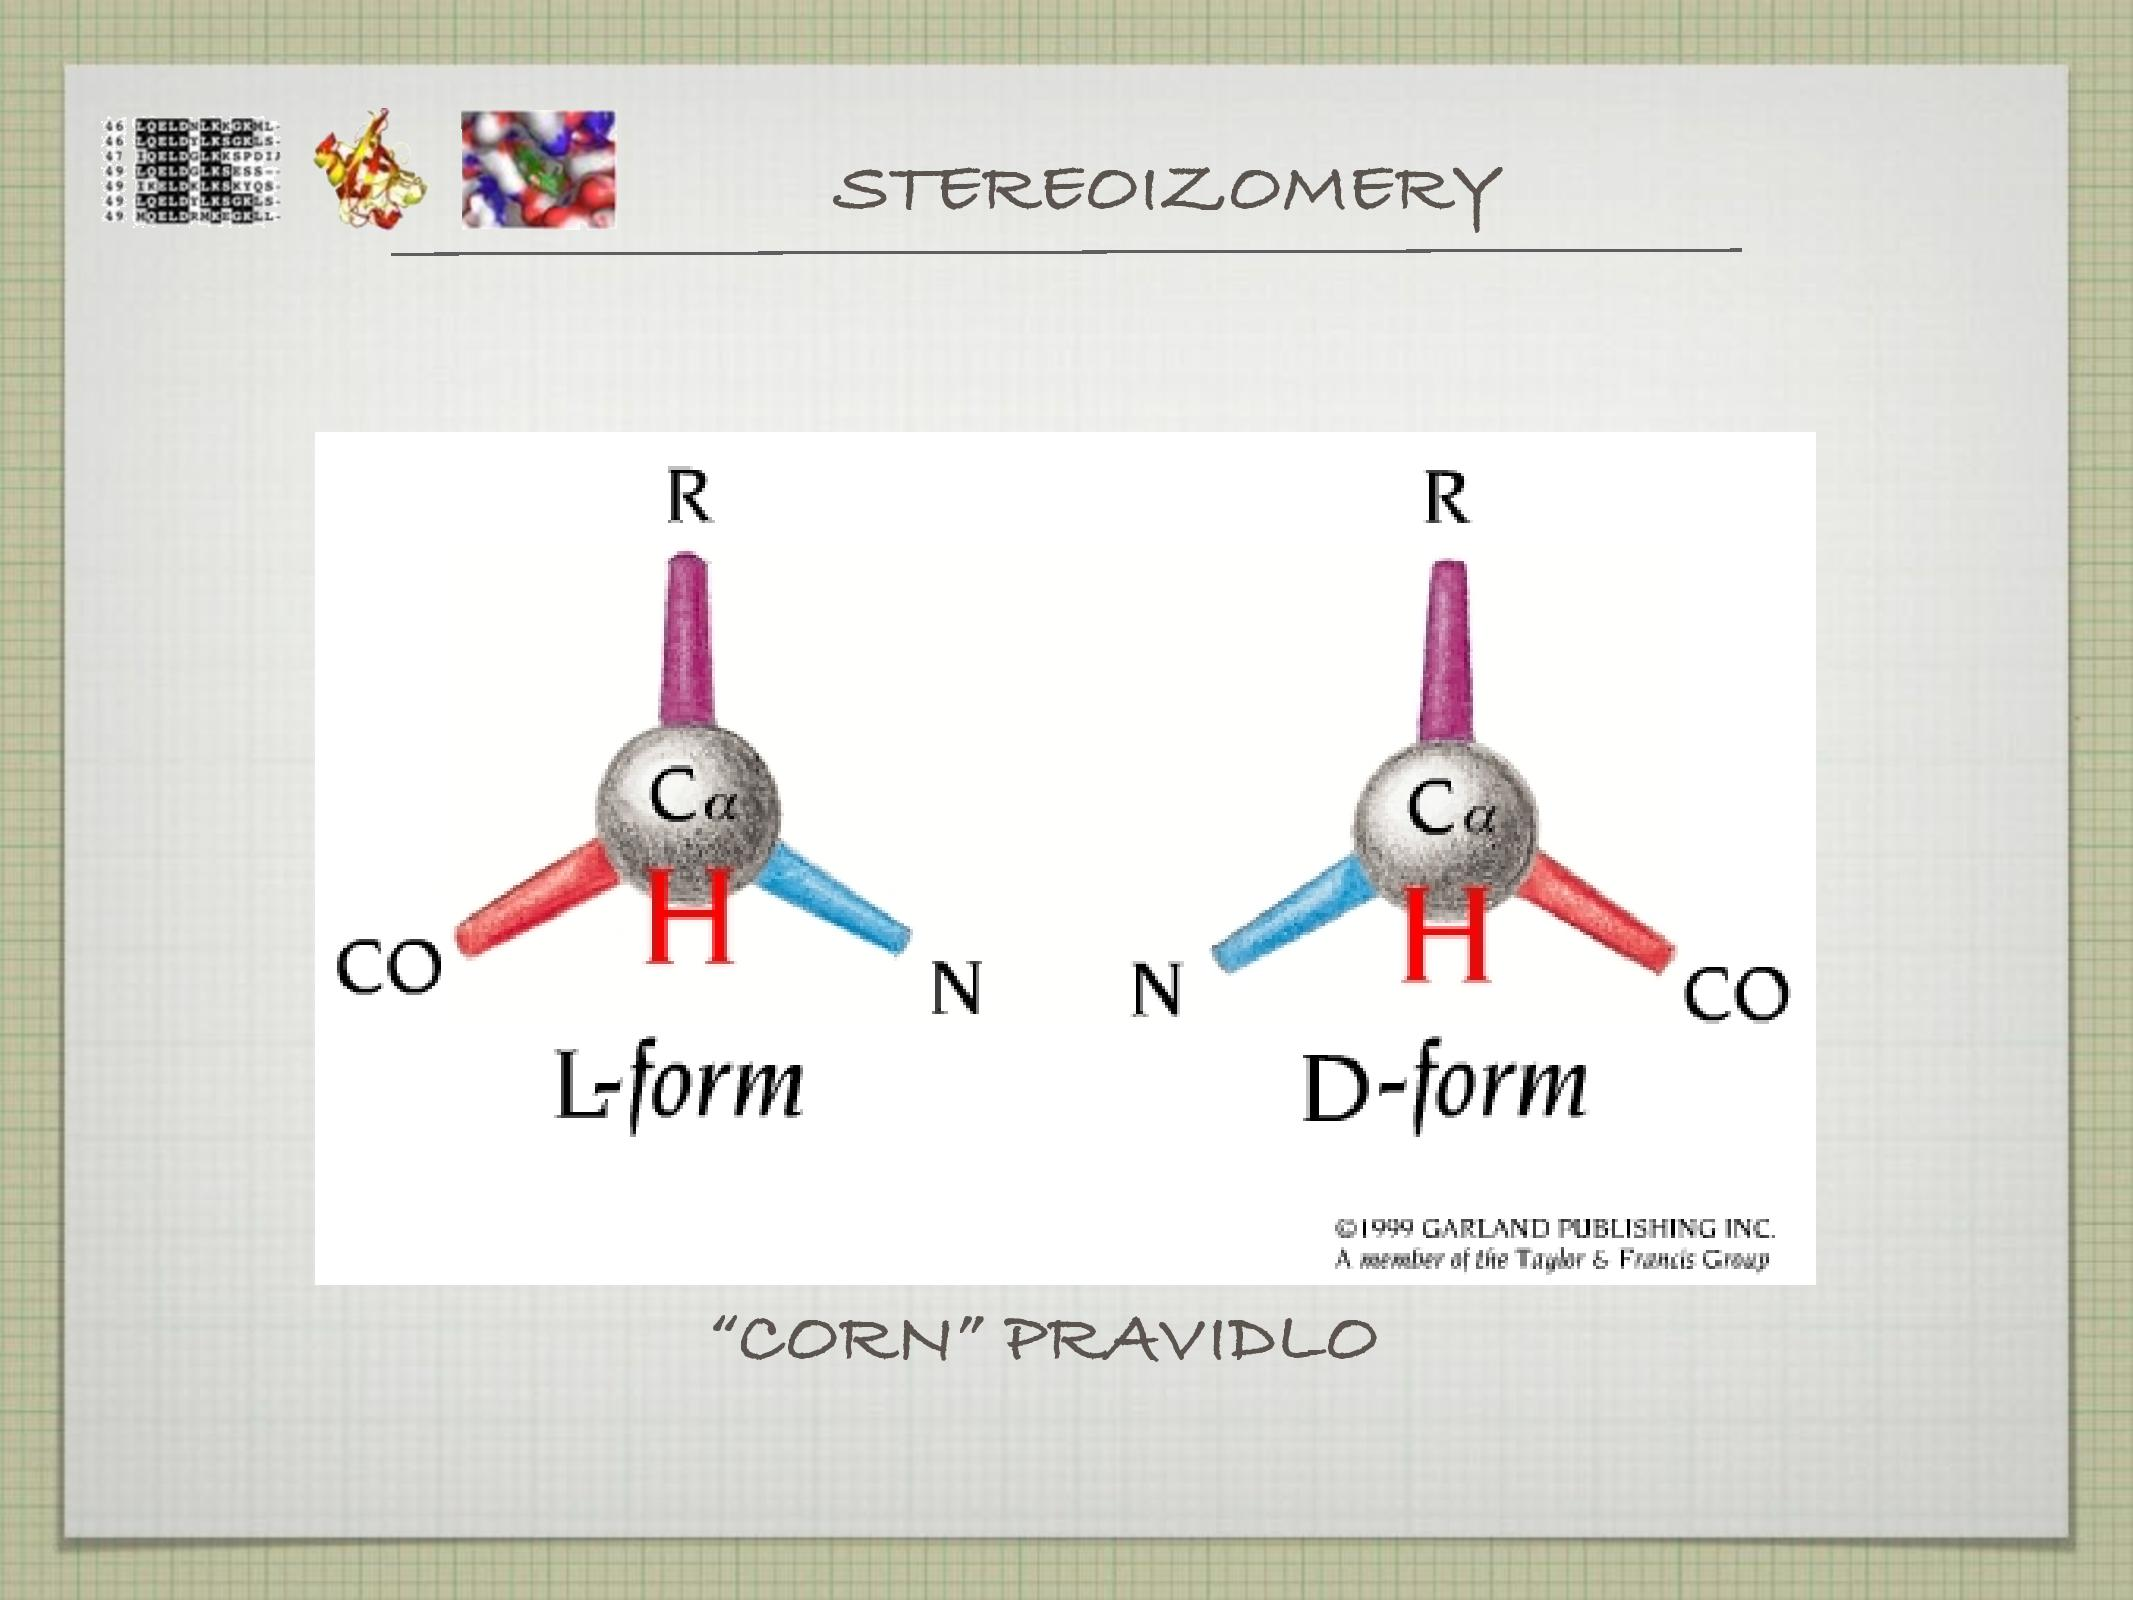
\includegraphics[width=0.85\textwidth]{slides-1/slide-23.jpg}
    \centering
    \label{slides-1-slide-23}
\end{figure}

\paragraph{Stereoizomery}
\begin{itemize}[nosep]
    \item chirální uhlík stáčí rovinu polarizovaného světla
    \item rozližujeme L a D enantiomery
\begin{itemize}[nosep]
    \item v laboratoři vznikají přibližně v poměru 1:1
    \item v živých organismech je většina AK druhu L
    \item buněčná stěna baterií bývá často D, aby nebyla rozpoznána jinými (imunitními/nepřátelskými) buňkami
\end{itemize}

\end{itemize}



\begin{figure}
    \caption{Prezentace č. 1, slide č. 26}
    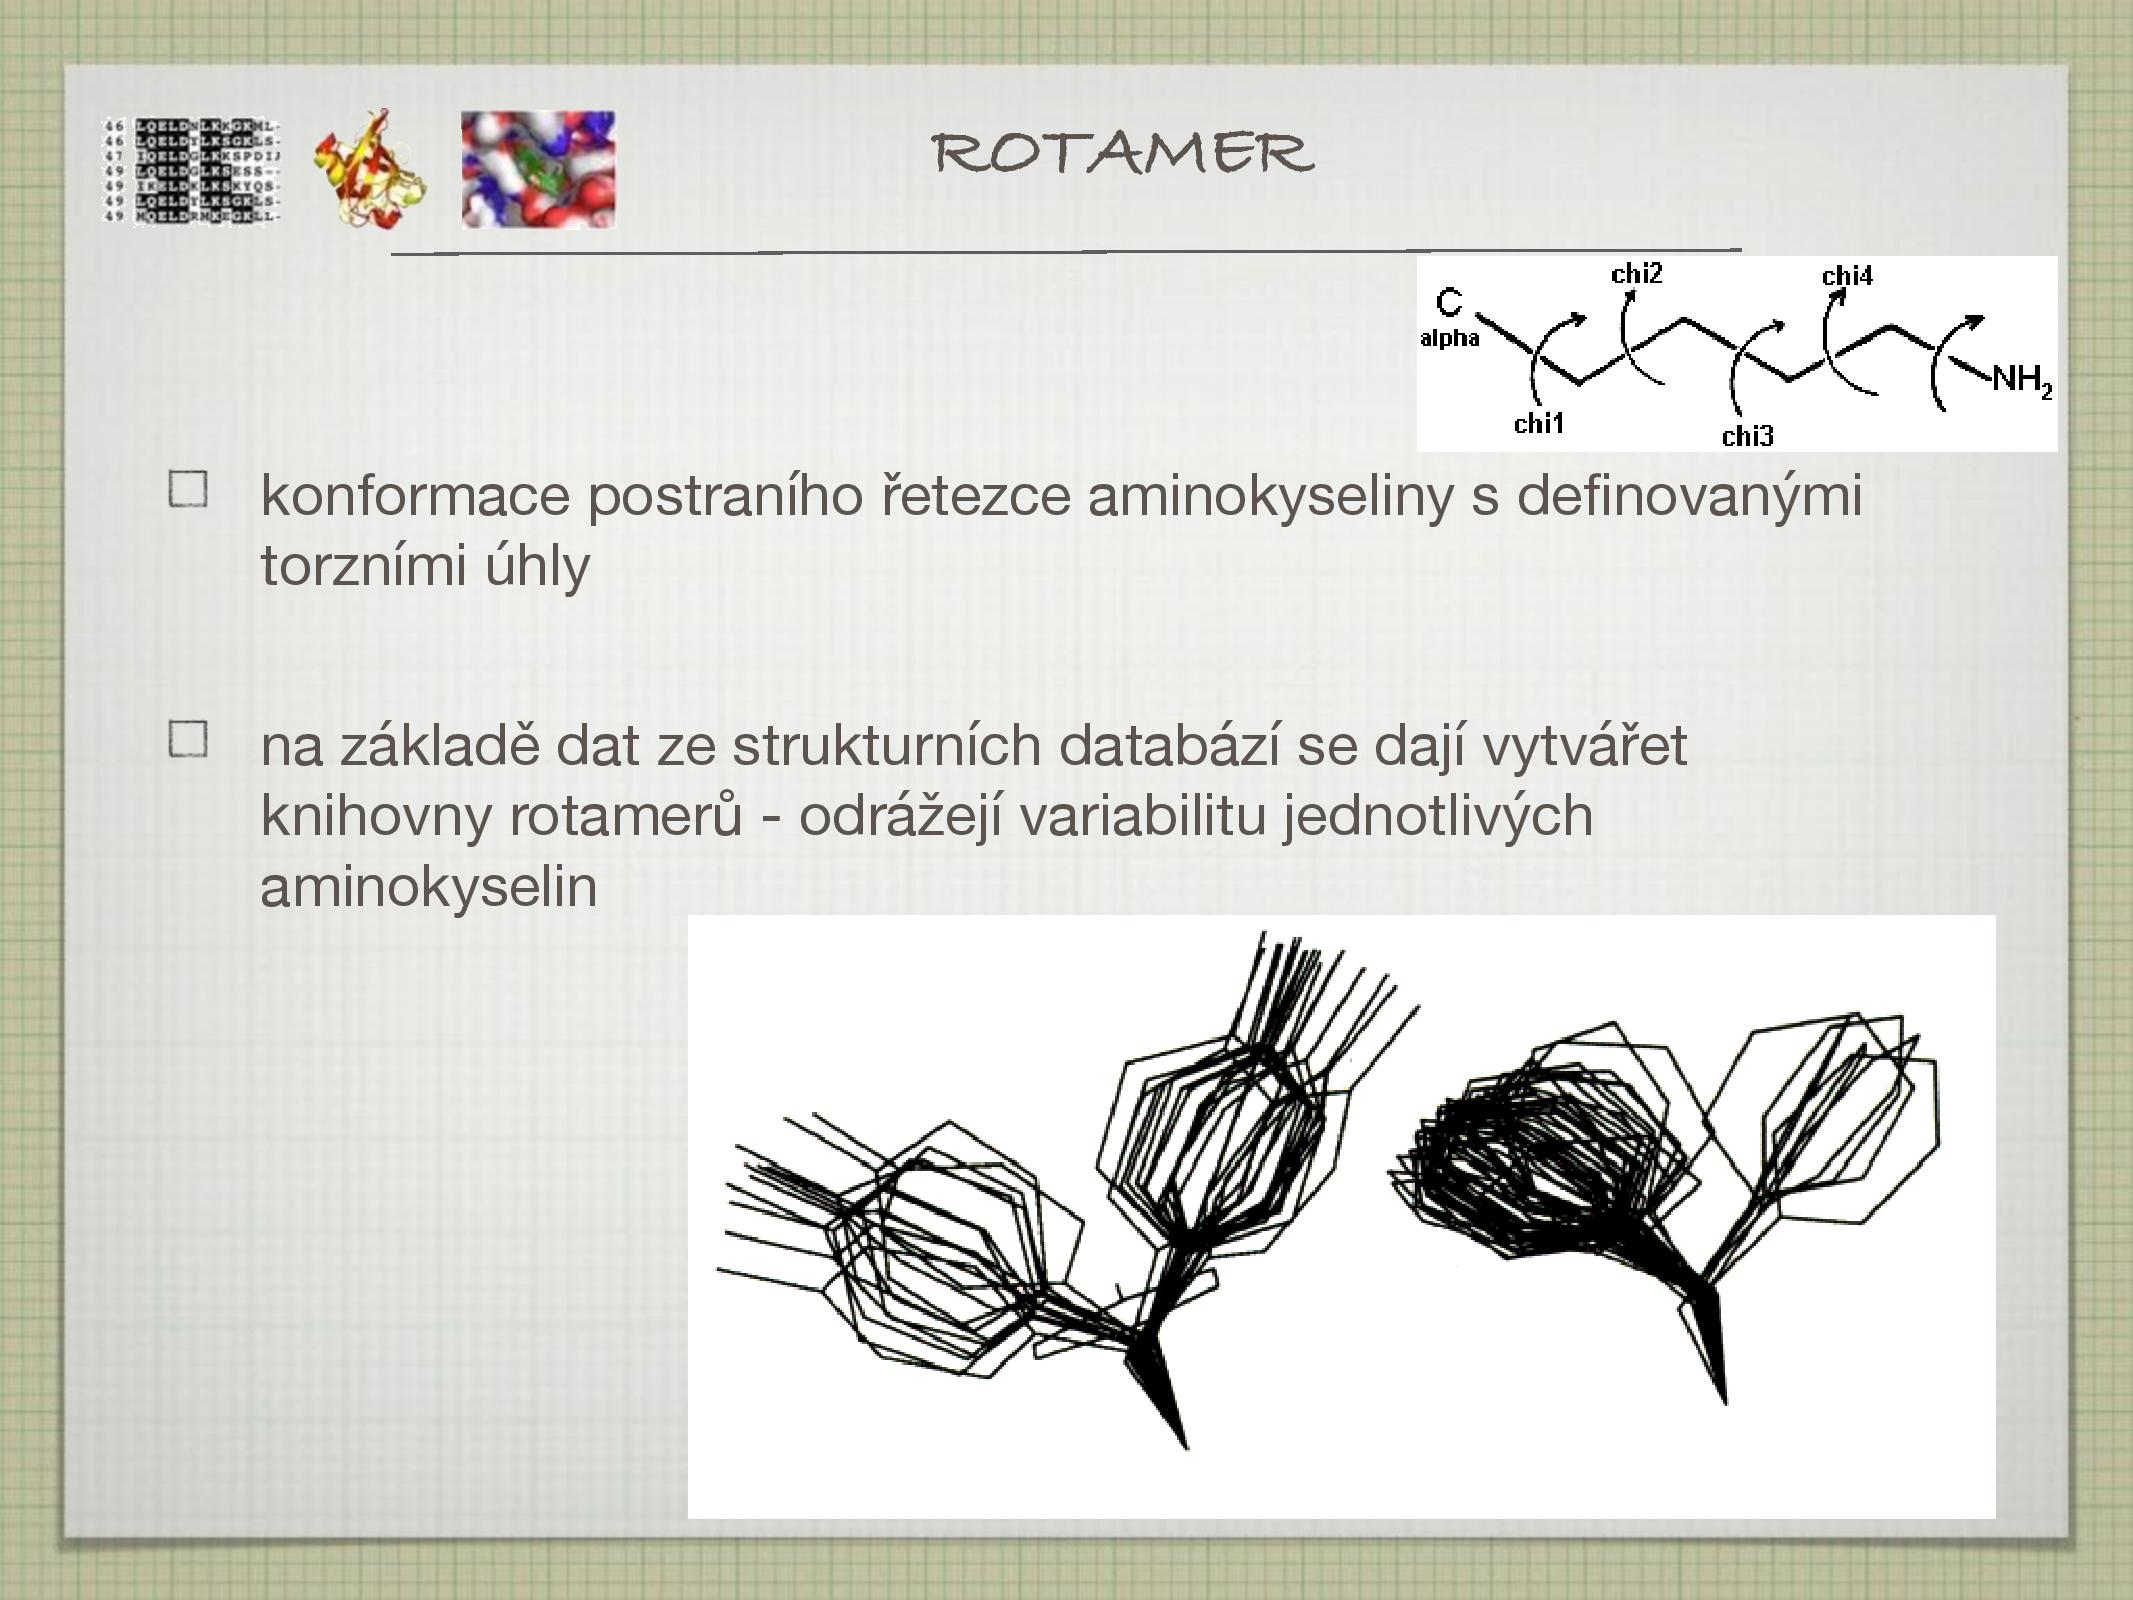
\includegraphics[width=0.85\textwidth]{slides-1/slide-26.jpg}
    \centering
    \label{slides-1-slide-26}
\end{figure}

\paragraph{Rotamery}
\begin{itemize}[nosep]
    \item rotamery jsou AK se stejným složením, u nichž se liší konformace jejich postranního řetězce
    \item vytváří se knihovny rotamerů (dle naměřených dat), odráží variabilitu jednotlivých AK
\end{itemize}



\begin{figure}
    \caption{Prezentace č. 1, slide č. 33}
    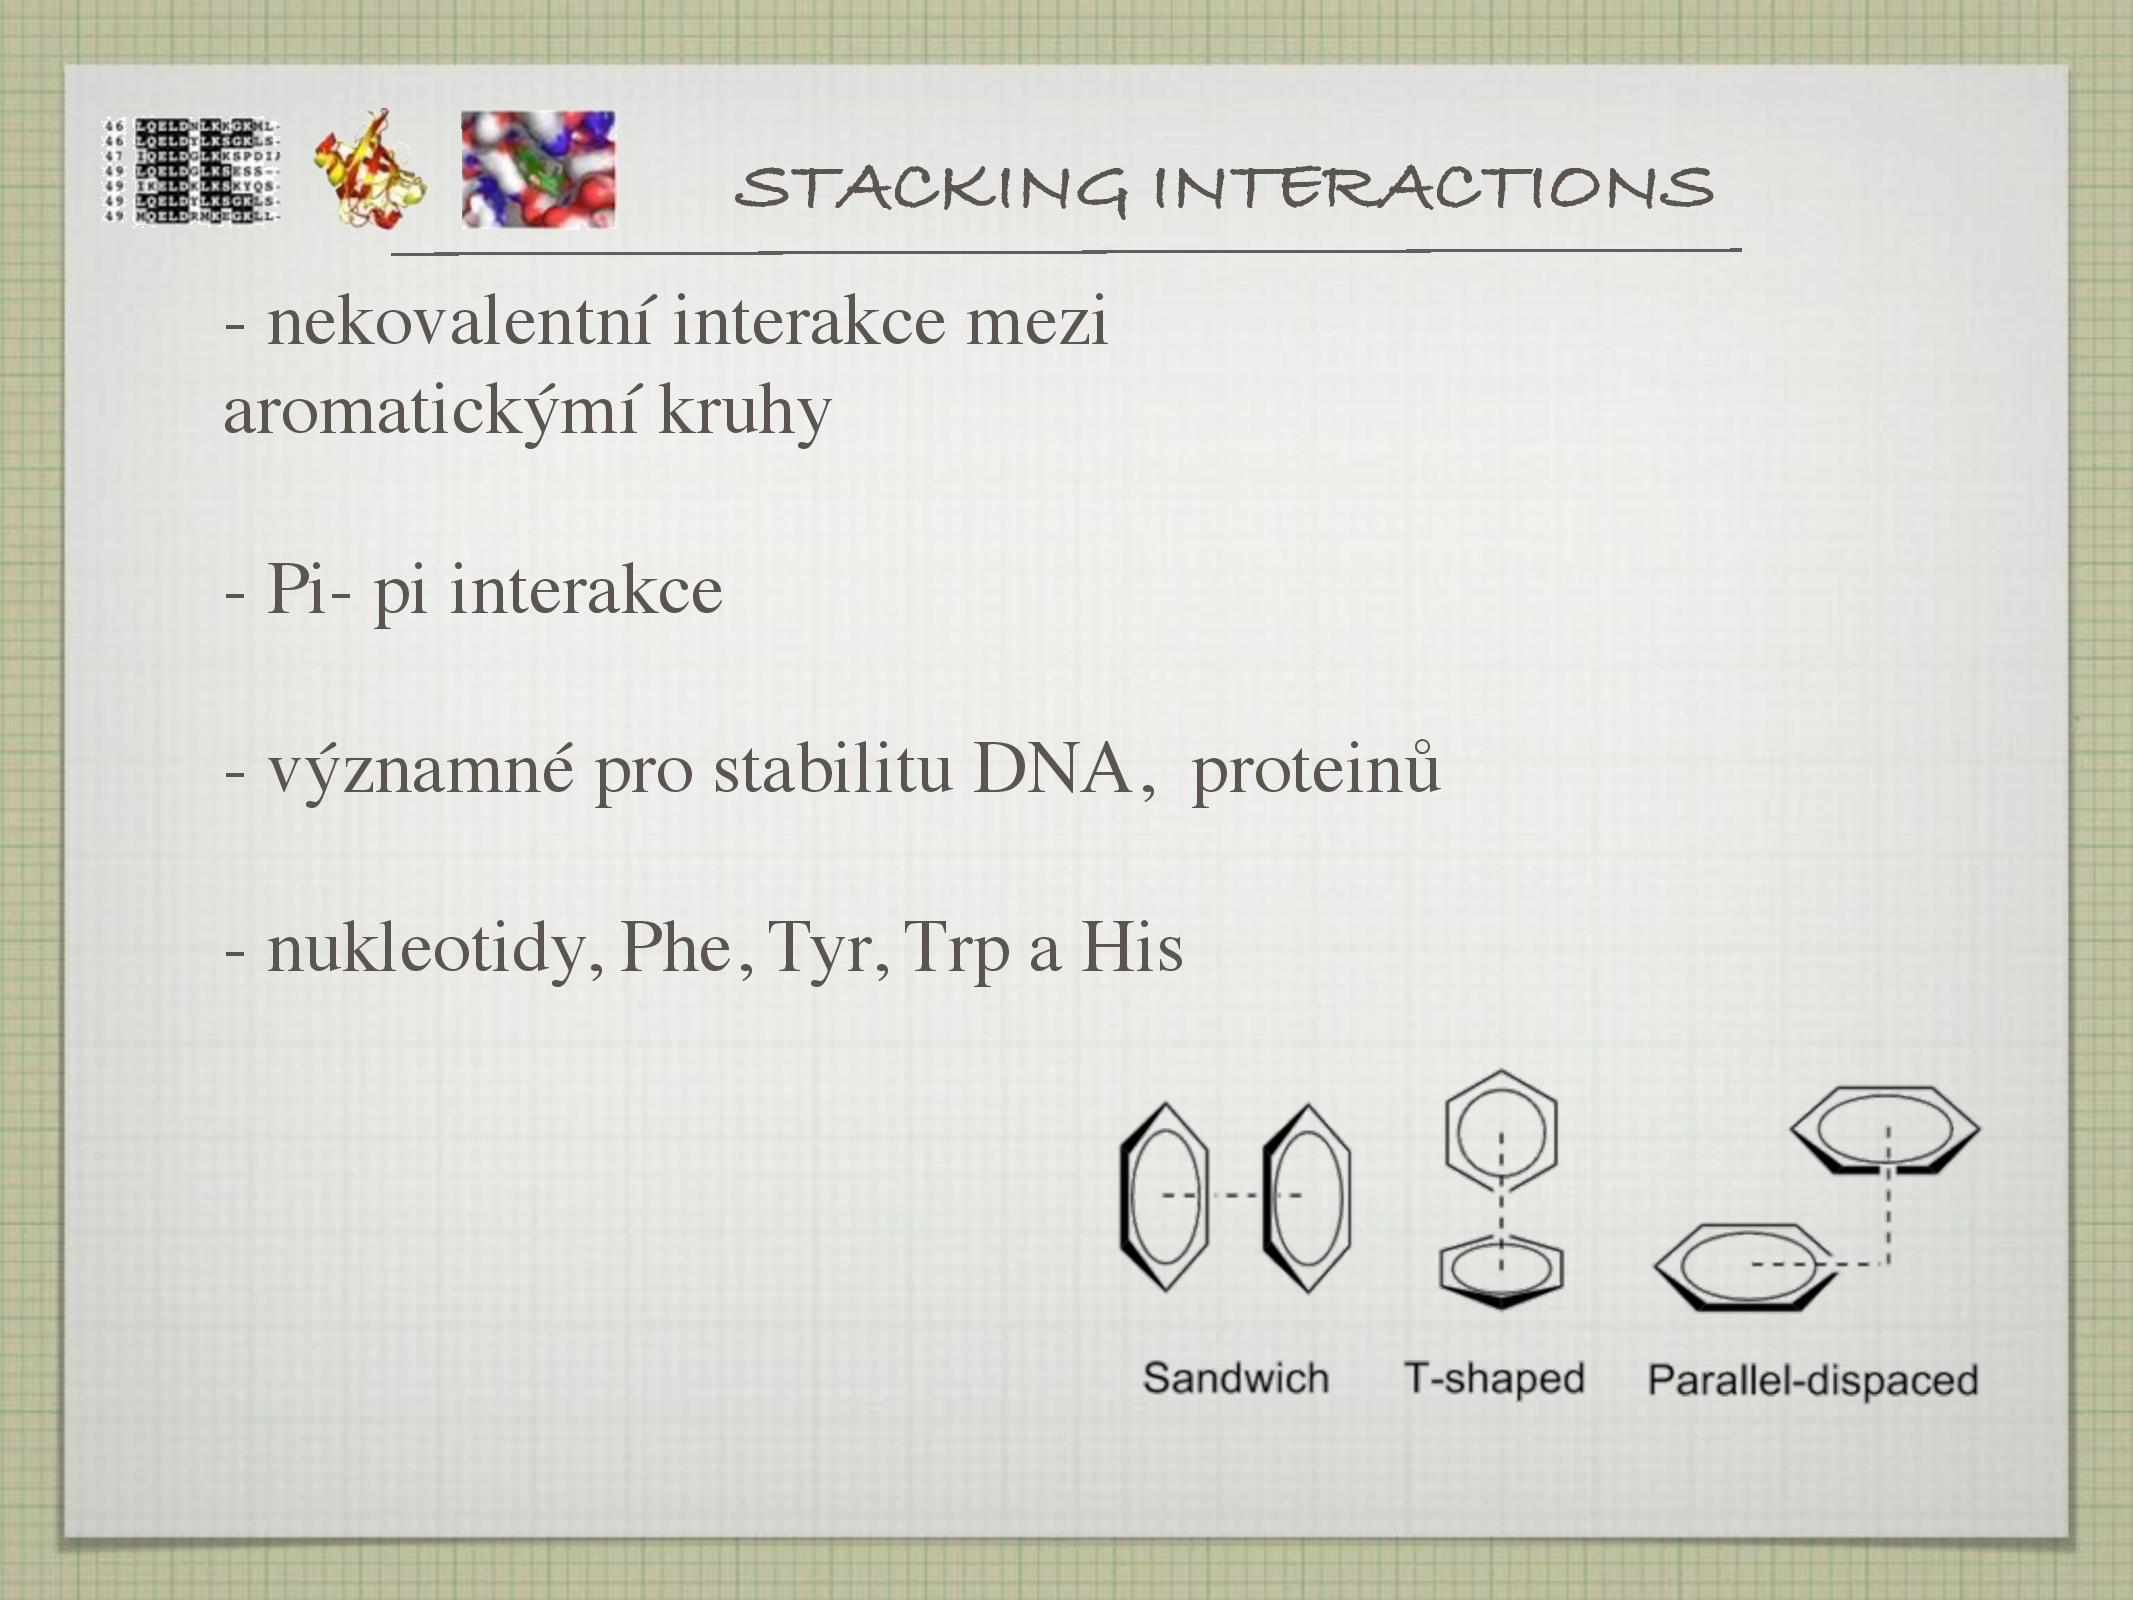
\includegraphics[width=0.85\textwidth]{slides-1/slide-33.jpg}
    \centering
    \label{slides-1-slide-33}
\end{figure}

\paragraph{Stacking interakce}
\begin{itemize}[nosep]
    \item interakce mezi aromatickými kruhy (\(\pi\)-\(\pi\) interakce)
    \item sandwich, T-shaped, parallel-displaced
    \item jsou významné pro stabilitu DNA i proteinů
\end{itemize}



\subsection{Seznam aminokyselin} \label{Seznam aminokyselin}


AK se dají rozdělit do několika skupin; nejdůlěžitější rozdělení je asi podle hydrofobicity, protože podle toho se poté jednotlivé AK vyskytují uvnitř nebo naopak na povrchu proteinů. Další významnou vlastností, která navíc s hydrofobicitou souvisí, je elektrický náboj.

\mybox{META}{Na zkoušku bude požadována znalost všech AK včetně jejich vzorce, vlastností, a zkratky.}


Polární AK jsou hydrofilní, nepolární jsou hydrofobní.

\begin{figure}
    \caption{Seznam aminokyselin a jejich rozdělení}
    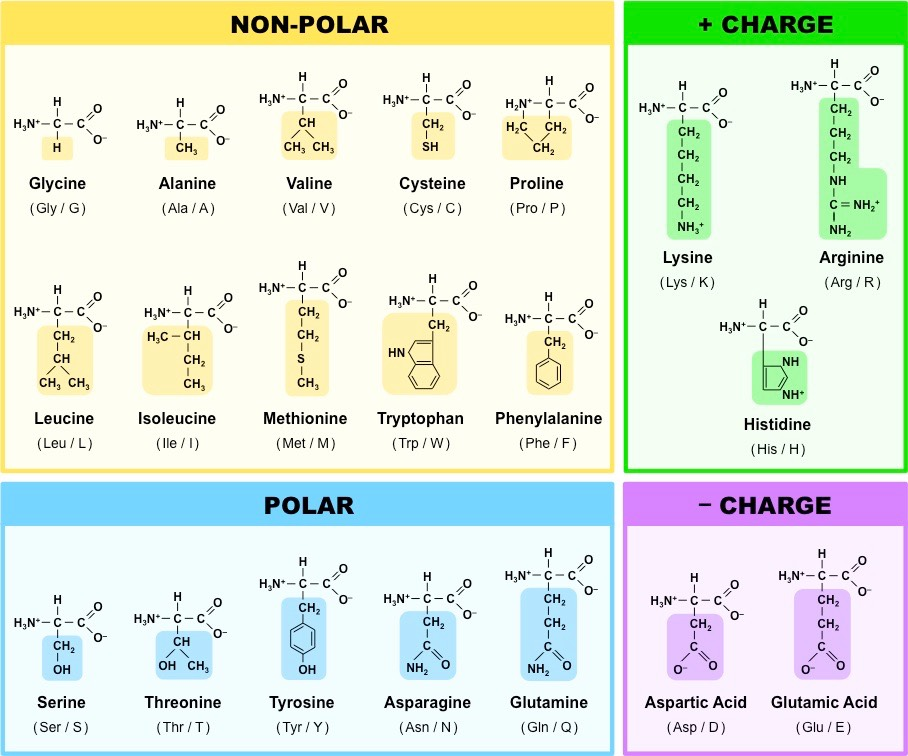
\includegraphics[width=0.85\textwidth]{ak.jpeg}
    \centering
    \label{}
\end{figure}


\mybox{AK s alifatickým postranním řetězcem}{\begin{description}
\item[glycin]\hfill \\
často v kolagenu, často ve smyčkách, nejmenší a tedy dobře konzervovaný


\item[alanin]\hfill \\
také velice častý, existuje i D forma (buněčná stěna, antibiotika), také velice malý a tedy dobře konzervovaný


\item[valin]\hfill \\
často v helixech a listech


\item[isoleucin]\hfill \\
má dva chirální atomy a tedy čtyři formy, je častý v helixech i listech


\item[leucin]\hfill \\
součástí leucinového zipu při interakci proteinů s DNA

\end{description}
}


\mybox{AK s kyselou (karboxylovou/amidovou) skupinou}{\begin{description}
\item[asparagová kyselina]\hfill \\
bývá v aktivních místech enzymů


\item[asparagin]\hfill \\
první izolovaná AK (z chřestu, viz jméno), tvoří vodíkové můstky, účastní se cappingu (neutralizuje parciální náboj na N' koncích alfa helixů)


\item[glutamová kyselina]\hfill \\
může fungovat jako neurotransmiter, je podobná ASP


\item[glutamin]\hfill \\
je zdrojem energie pro mozek

\end{description}
}


\mybox{AK se zásaditou (aminovou) skupinou}{\begin{description}
\item[arginin]\hfill \\
může být methylován, bývá na povrchu, kvůli kladného náboje tvoří vodíkové můstky se záporně nabitými strukturami (DNA)


\item[lysin]\hfill \\
může být postrtranslačně modifikován

\end{description}
}


\mybox{AK s aromatickým jádrem nebo hydroxylovou skupinou}{\begin{description}
\item[histidin]\hfill \\
tvoří imidazol (další nukleotid, někdy součástí wobblingu), má neutrální pKa --- malá změna pH vede he změně náboje, takže je často používán jako vypínač závislý na pH, účastní se koordinace kovů


\item[fenyalanin]\hfill \\
je prekurzorem neurotransmiterů


\item[serin]\hfill \\
katalyzuje reakce (je to alkohol), především O-glykosylace a fosforylace, nervové plyny jej blokují v acetylcholinesteráze


\item[threonin]\hfill \\
má dva chirální atomy, taktéž účasten O-glykosylace a fosforylace (je to alkohol)


\item[tyrosin]\hfill \\
podobný PHE, prekurzor neurotransmiterů, účasten forsforylací (je to alkohol)


\item[tryptofan]\hfill \\
je největší a tedy dobře konzervovaný, účasten hydrofóbních interakcí (s cukry), prekurzor serotoninu a niacinu

\end{description}
}


\mybox{AK se sírou v postranním řetězci}{\begin{description}
\item[methionin]\hfill \\
má jen jeden kodon, může být na povrchu oxidován


\item[cystein]\hfill \\
často v hydrofobním jádře protein§ (přestože je polární), tvoří disulfidické můstky, iteraguje s ionty kovů (často v aktivních místech enzymů)

\end{description}
}


\mybox{AK obsahující sekundární amin}{\begin{description}
\item[prolin]\hfill \\
nemá vodík na dusíku => netvoří vodíkové můstky, nebývá v alfa-helixech ani listech

může být i v konformaci cis (většinou uhlovodíková zbytek AK bývá trans) => může fungovat jako vypínač, protože mění konformaci

jeho cyklus je extrémě rigidní, tvoří zlomy v proteinech

\end{description}
}



Pro popis aminokyselin se někdy využívá i \emph{B} (Asn/Asp) a \emph{Z} (Gln/Glu). Kromě výše zmíněných dvaceti AK se vydělují ještě následující dvě.

\begin{figure}
    \caption{Prezentace č. 1, slide č. 49}
    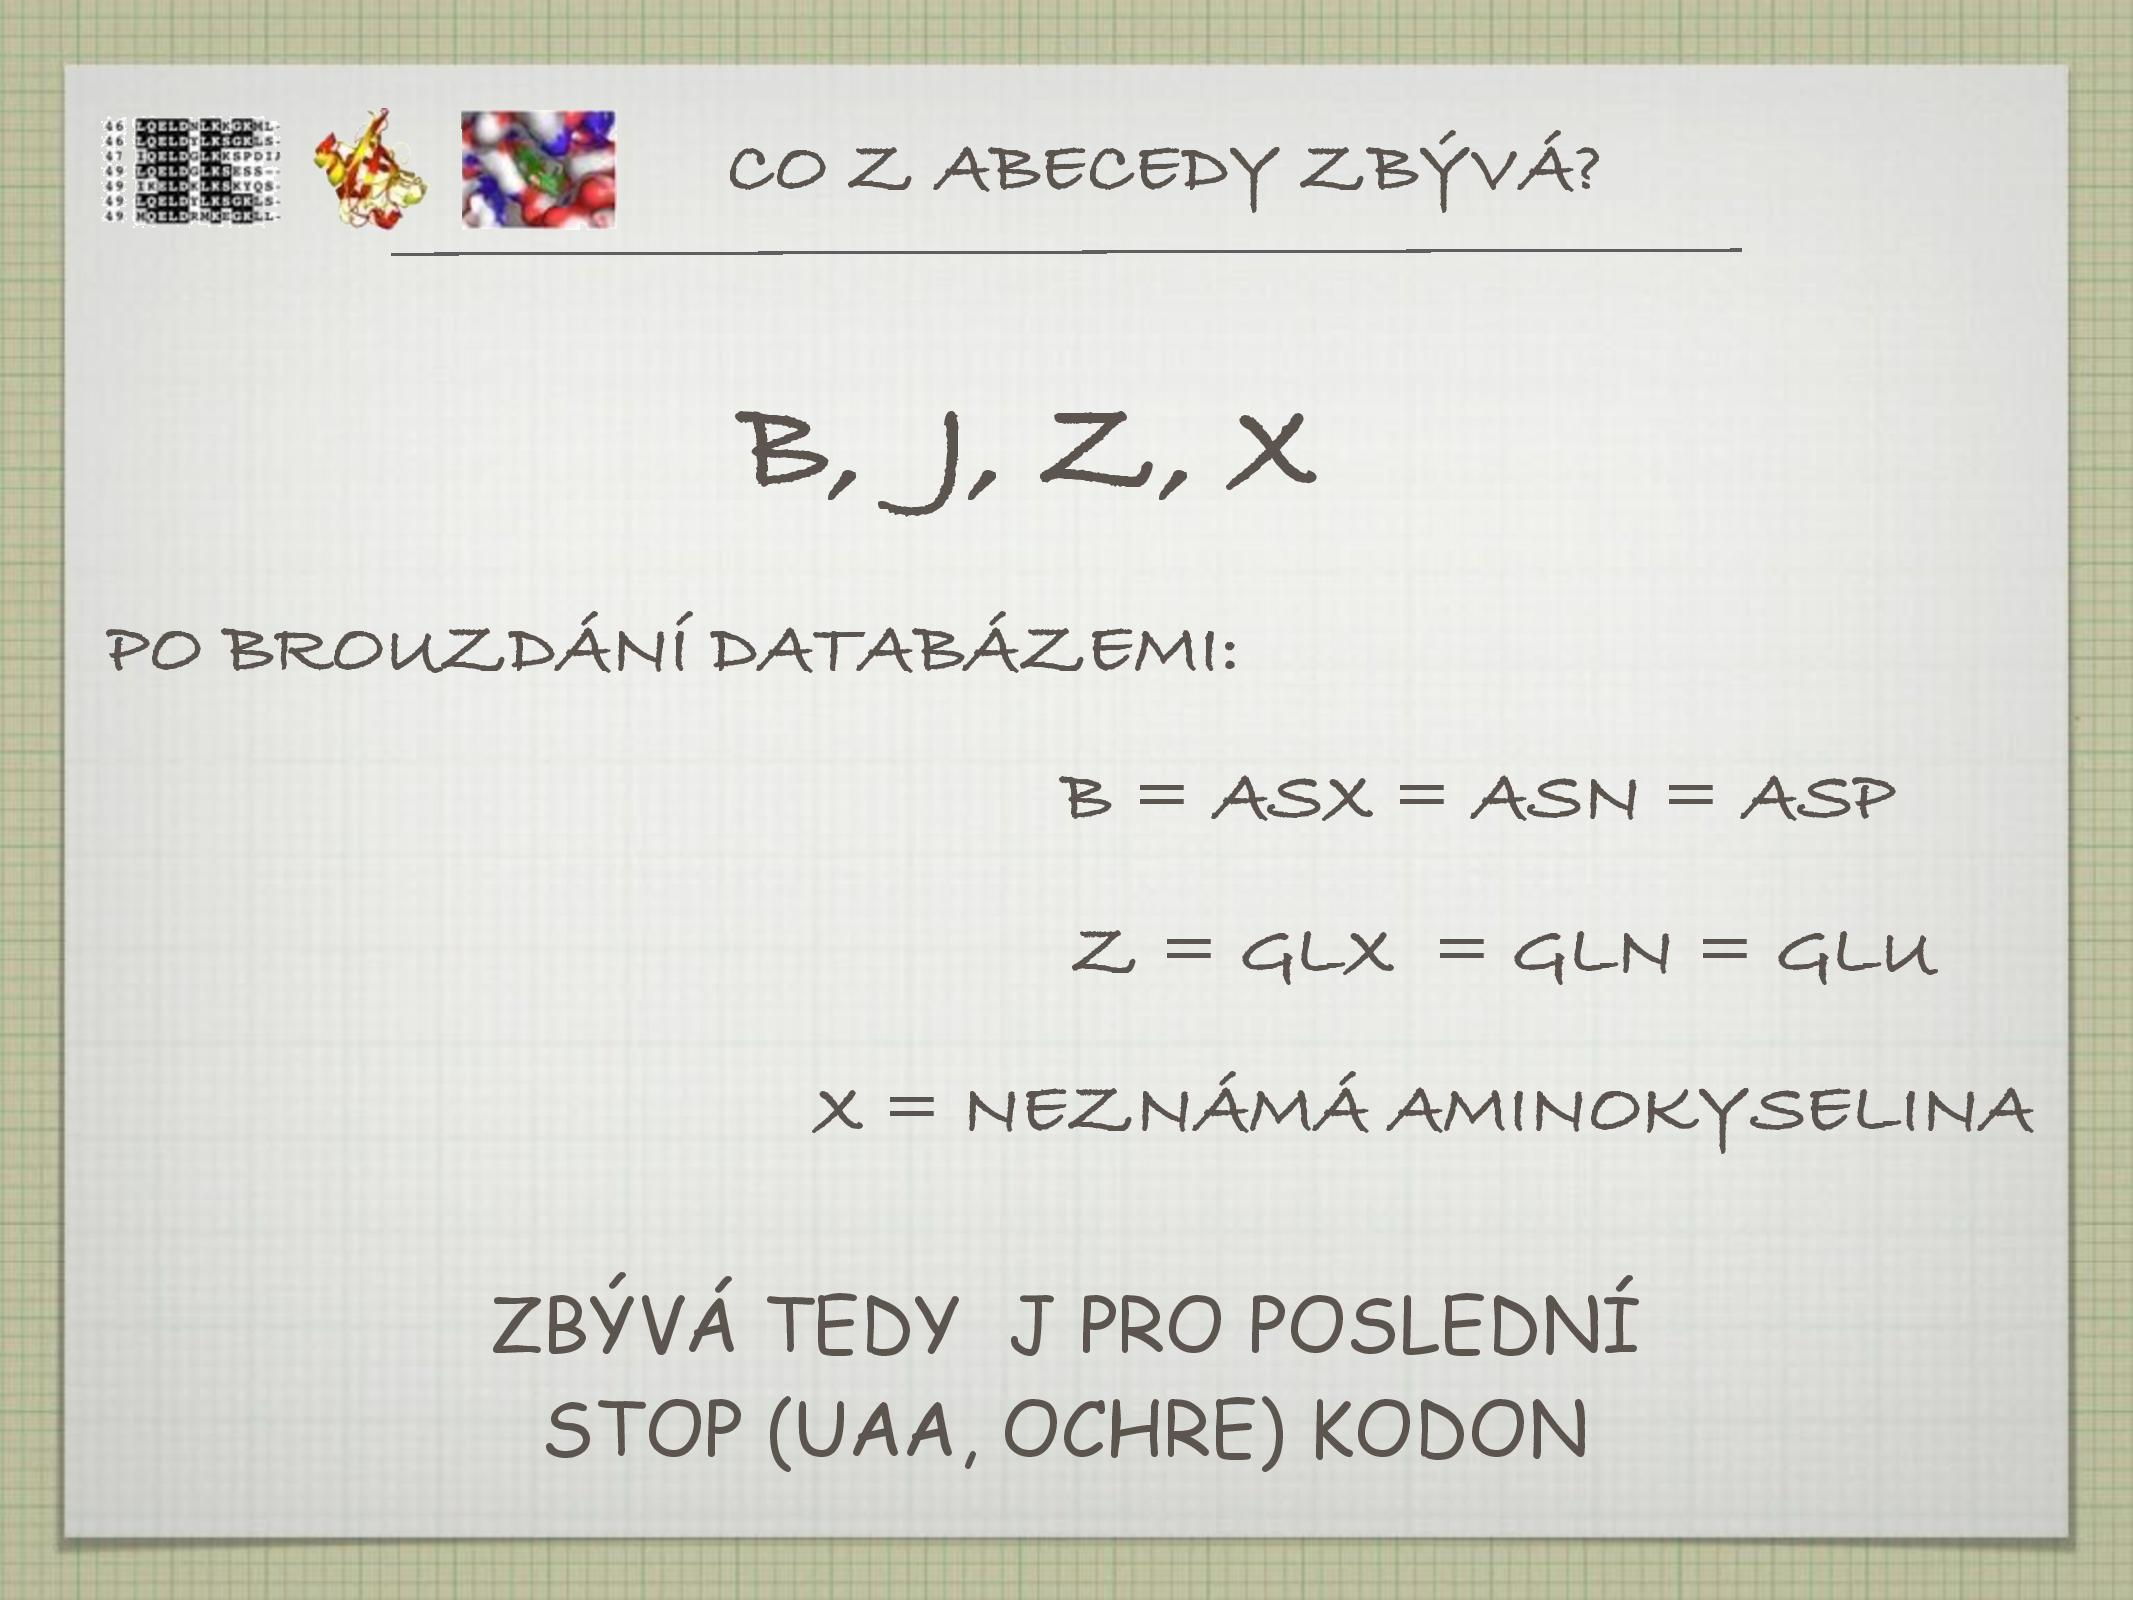
\includegraphics[width=0.85\textwidth]{slides-1/slide-49.jpg}
    \centering
    \label{slides-1-slide-49}
\end{figure}

\begin{description}
\item[pyrolysin]\hfill \\
kódovaný UAG stop kodonem


\item[selenocystein]\hfill \\
kódovaný UGA stop kodonem, využíván pro určení struktury proteinů, je v řadě enzymů

\end{description}


\section{Další proteinové struktury} \label{Další proteinové struktury}


Kromě primární struktury proteinu rozlišujeme ještě sekundární, teriární a kvarterní. Sekundární struktura proteinu je určena lokálními konformacemi jeho částí.

\begin{figure}
    \caption{Prezentace č. 1, slide č. 55}
    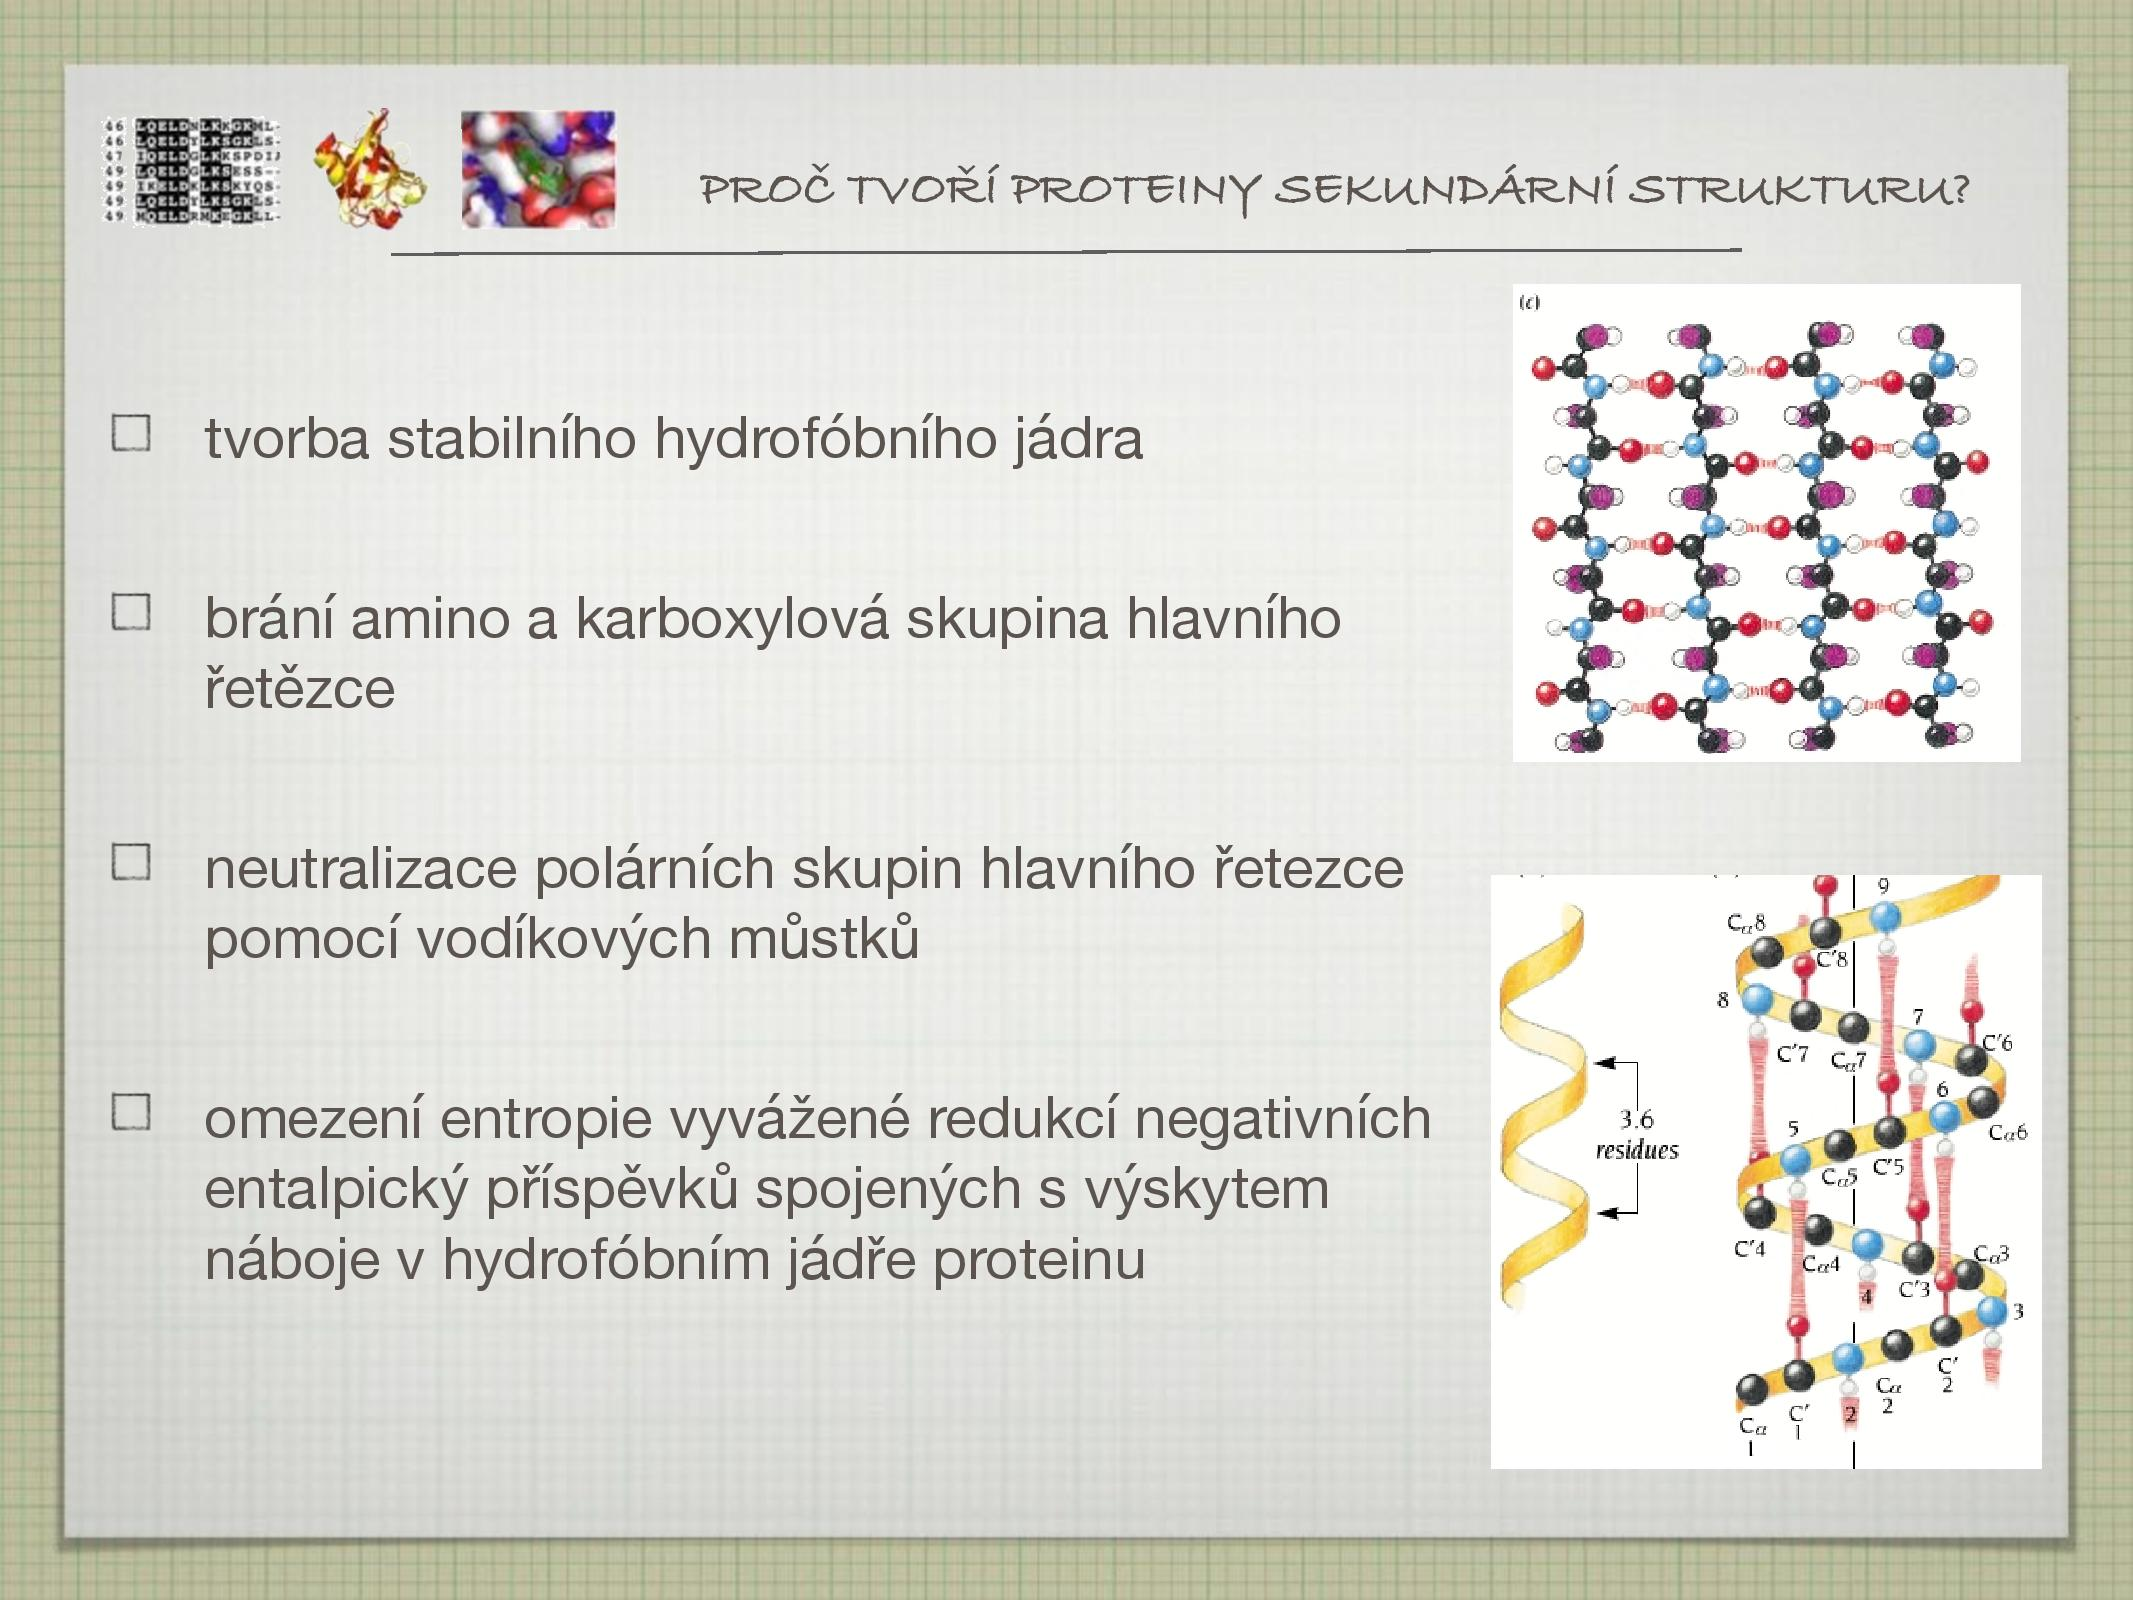
\includegraphics[width=0.85\textwidth]{slides-1/slide-55.jpg}
    \centering
    \label{slides-1-slide-55}
\end{figure}

\paragraph{Důvody vzniku}
\begin{itemize}[nosep]
    \item snaha o tvorbu stabilního hydrofobního jádra
\begin{itemize}[nosep]
    \item důvod: entropie klesne, ale tento pokles je vyvážen růstem entalpie, která je negativně ovlivněná výskytem náboje v jádře proteinu
    \item způsob: neutralizace polárních amino a karboxylových skupin na hlavním řětězci vznikem vodíkových můstků
\end{itemize}

\end{itemize}



\paragraph{Vodíková vazba a stabilizace}
\begin{itemize}[nosep]
    \item síla vodíkové vazby závisí n atypu atomu a geometrii vazby
\begin{itemize}[nosep]
    \item cca 1--60 kJ/mol, v proteinech většinou okolo 10 kJ/mol
    \item se zvětšujícím se úhlem vazby klesá její síla: odklon o 20\(^{\circ}\) snižuje energii o 10\%
\end{itemize}

\end{itemize}



\begin{figure}
    \caption{Prezentace č. 1, slide č. 57}
    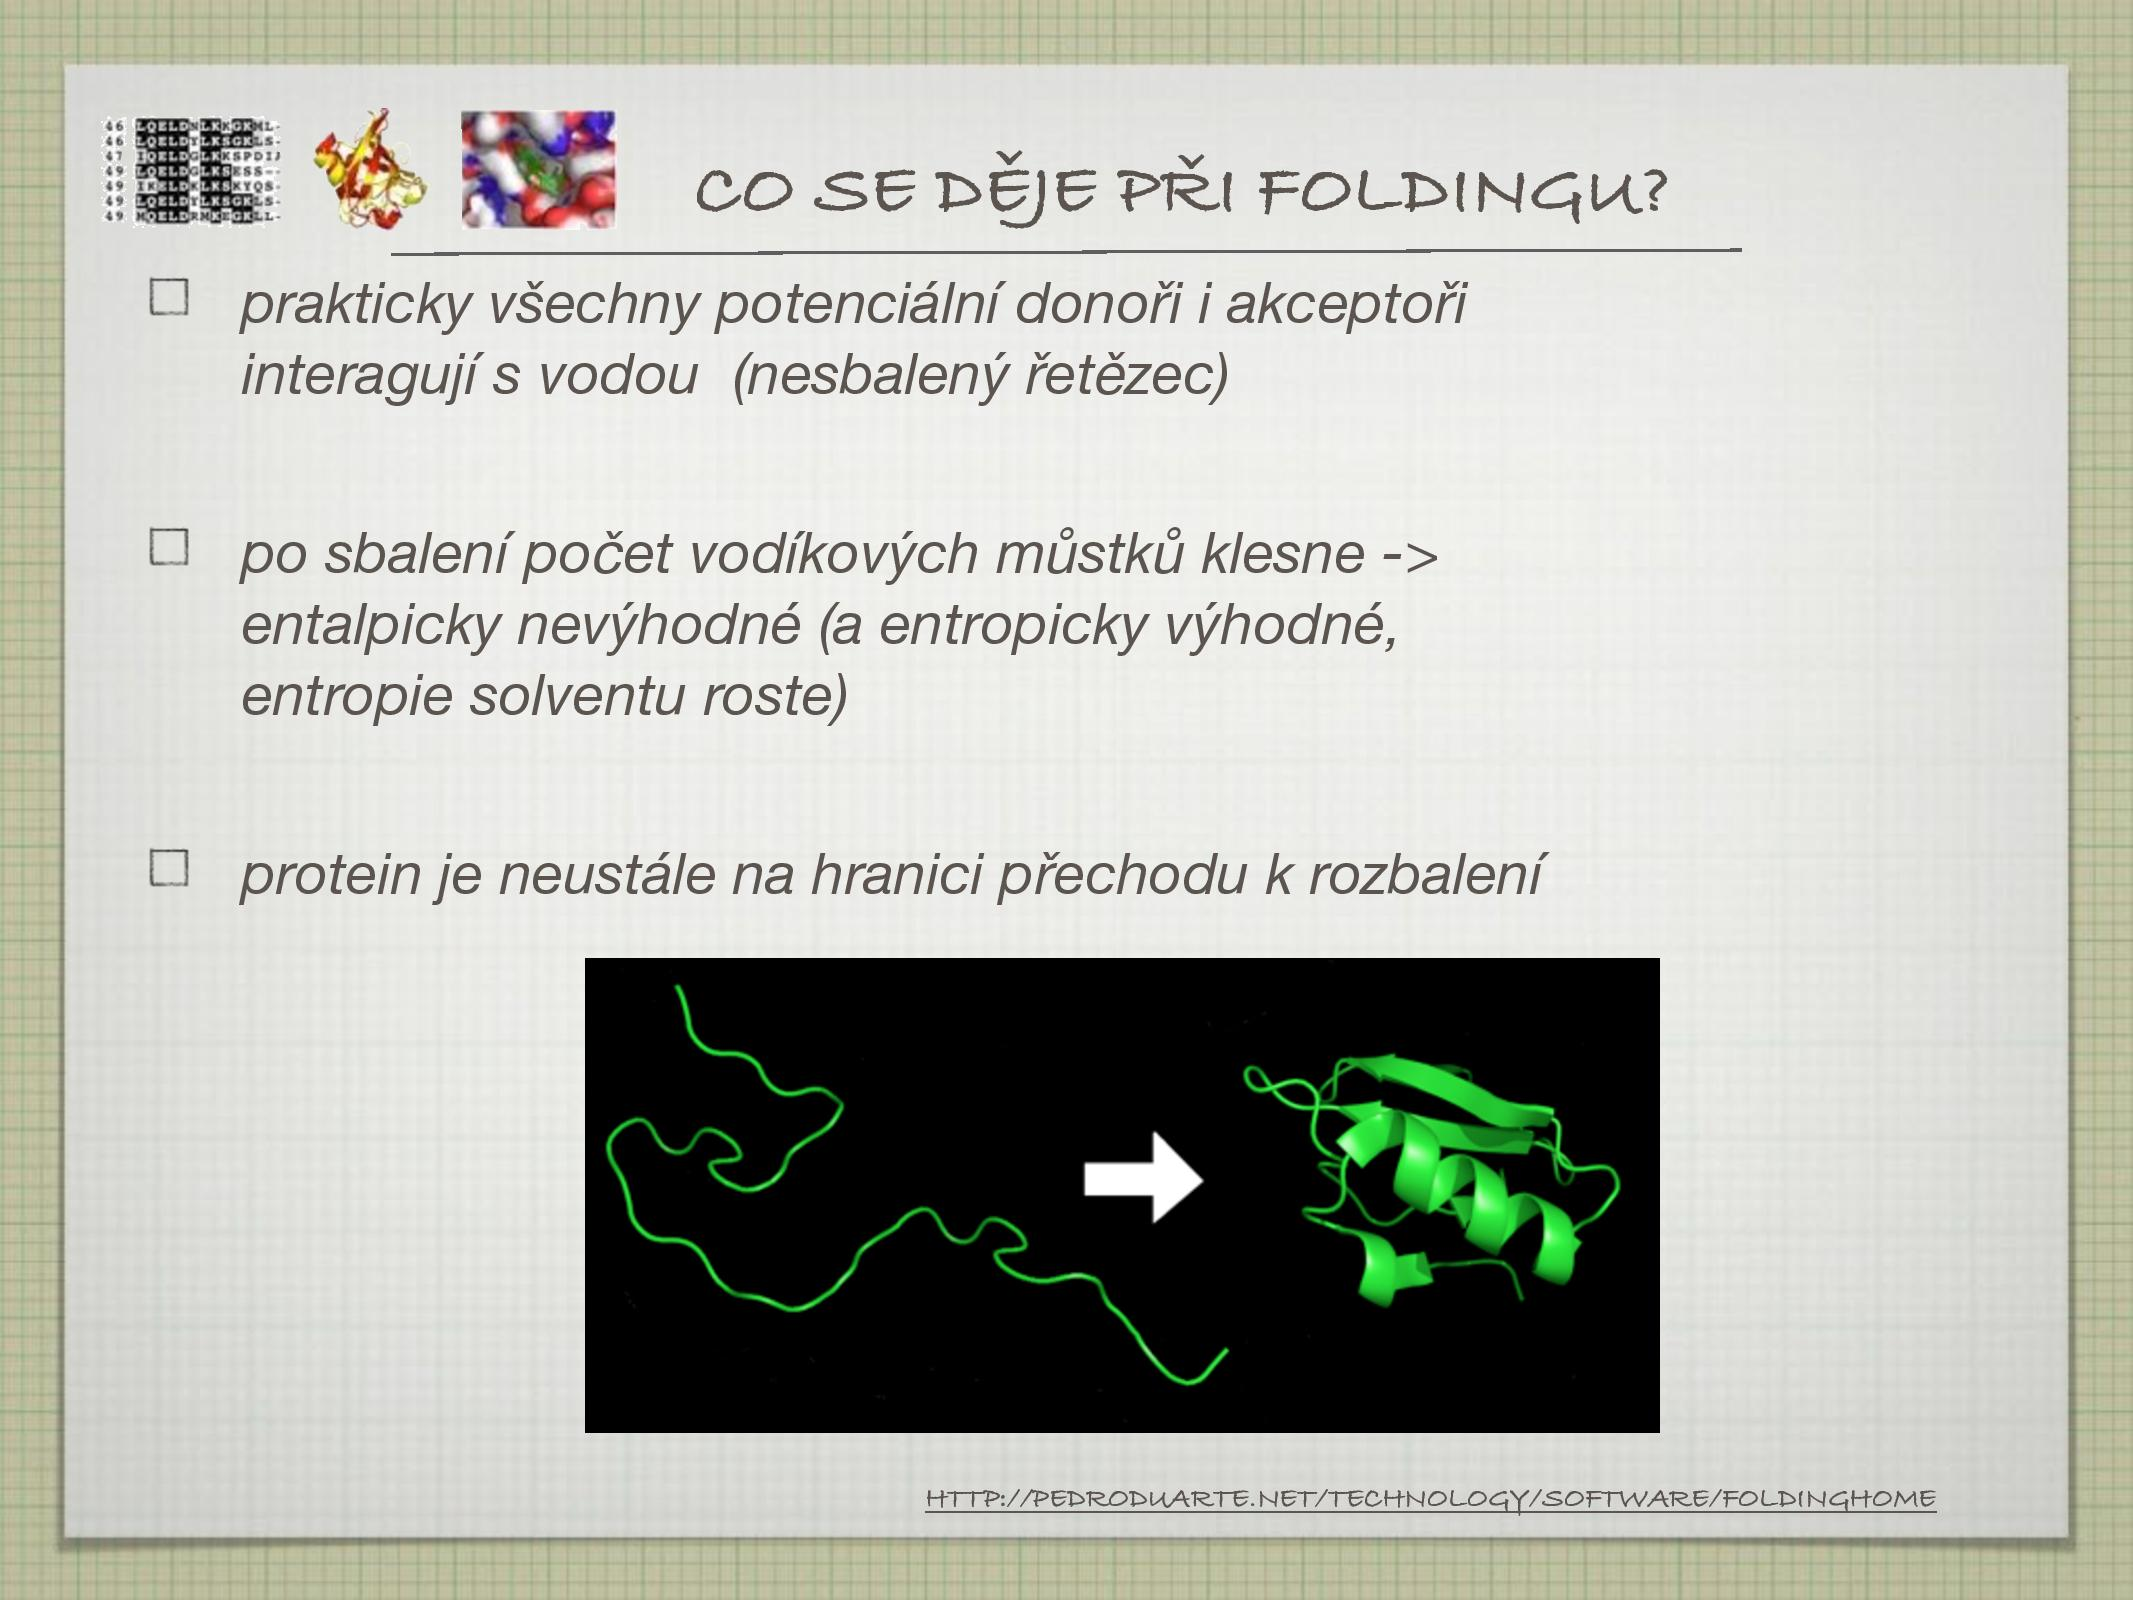
\includegraphics[width=0.85\textwidth]{slides-1/slide-57.jpg}
    \centering
    \label{slides-1-slide-57}
\end{figure}

\paragraph{Folding}
\begin{enumerate}[nosep]
    \item protein je nesbalený, všichni donoři i akceptoři reagují s vodou
    \item protein se sbalí, počet vodíkových můstků klesne
\begin{itemize}[nosep]
    \item entalpicky nevýhodné, ale entropicky výhodné
\end{itemize}

    \item protein je nyní neustále na hranici rozbalení, aby bylo možné jej případně rozložit (a nezůstal v buňce napořád)
\end{enumerate}



\begin{figure}
    \caption{Prezentace č. 1, slide č. 59}
    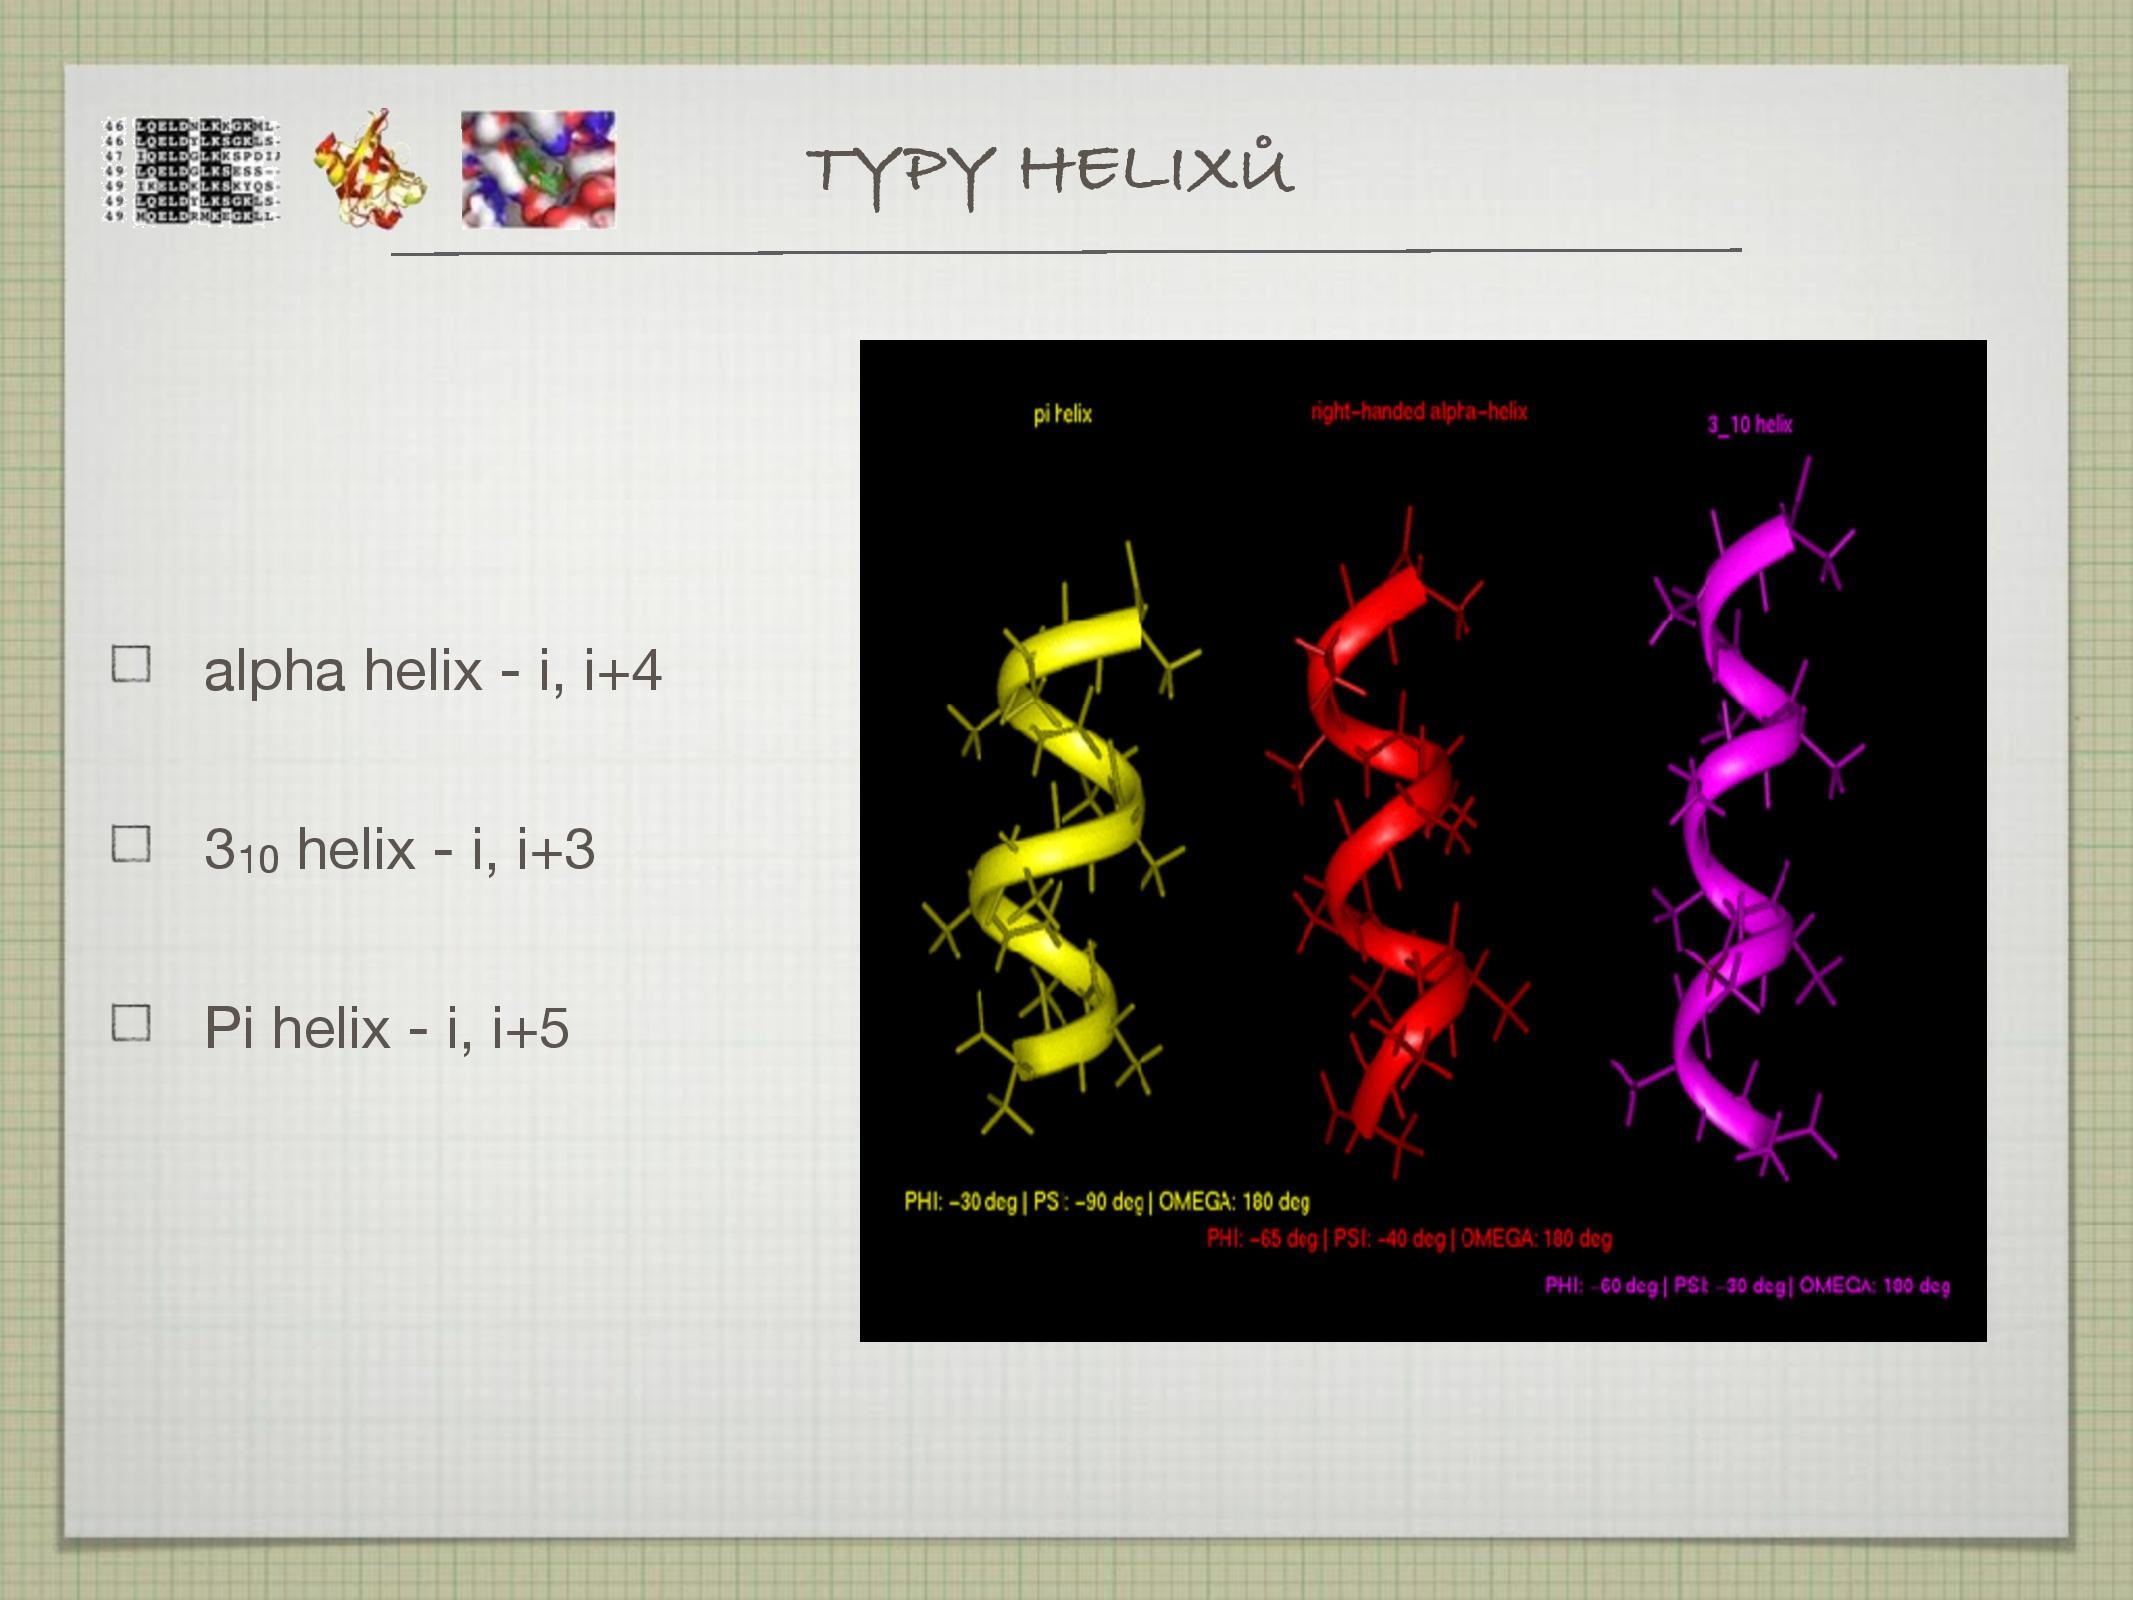
\includegraphics[width=0.85\textwidth]{slides-1/slide-59.jpg}
    \centering
    \label{slides-1-slide-59}
\end{figure}
\begin{figure}
    \caption{Prezentace č. 1, slide č. 60}
    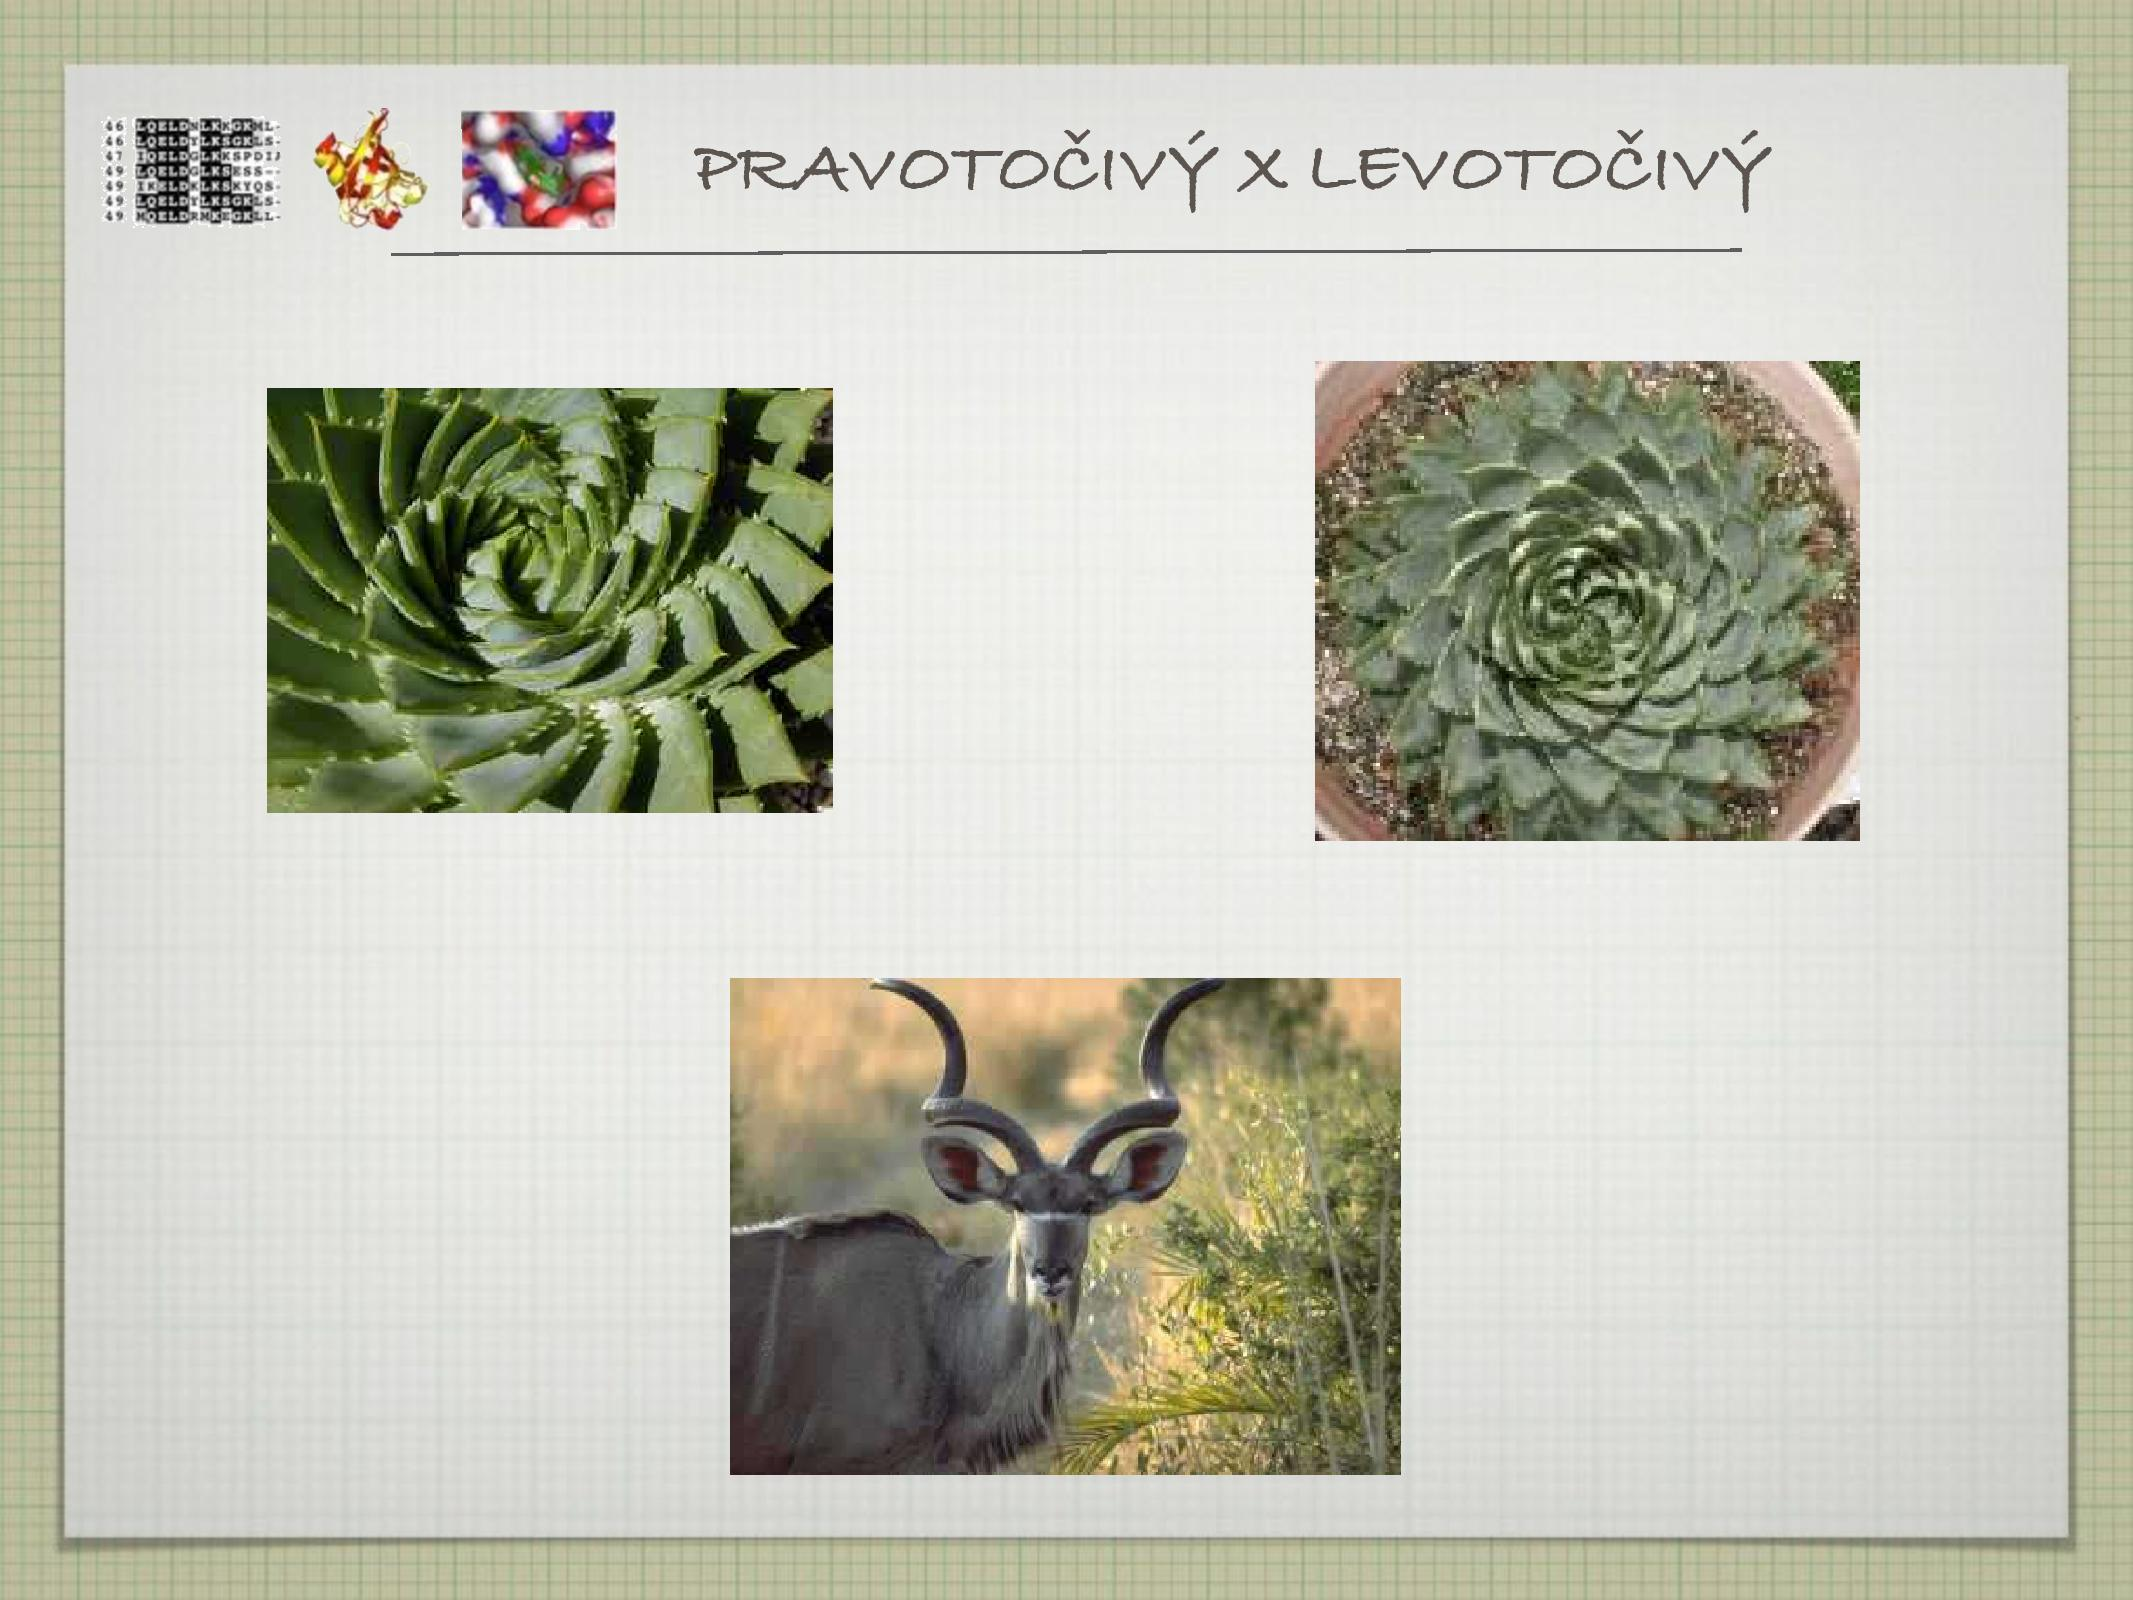
\includegraphics[width=0.85\textwidth]{slides-1/slide-60.jpg}
    \centering
    \label{slides-1-slide-60}
\end{figure}

\paragraph{Helix}
\begin{itemize}[nosep]
    \item teoreticky popsaný Linusem Paulingem
    \item model potvrzen strukturou myoglobinu
    \item může být levotočivý (Ala, Leu, Val) i pravotočivý (Gly, Pro)
    \item několikero druhů
\begin{itemize}[nosep]
    \item \(\alpha\) helix, nad sebou jsou AK \(i\) a \(i + 4\)
    \item \(3_{10}\) helix, nad sebou jsou AK \(i\) a \(i + 3\)
    \item \(\pi\) helix, nad sebou jsou AK \(i\) a \(i + 5\)
\end{itemize}

    \item zobrazování pomocí helix-wheel diagramu
\begin{itemize}[nosep]
    \item barvení podle typu AK
    \item všechny hydrofilní budou na jedné straně, hydrofobní na druhé (vznik snopců)
\end{itemize}

\end{itemize}



\begin{figure}
    \caption{Prezentace č. 1, slide č. 63}
    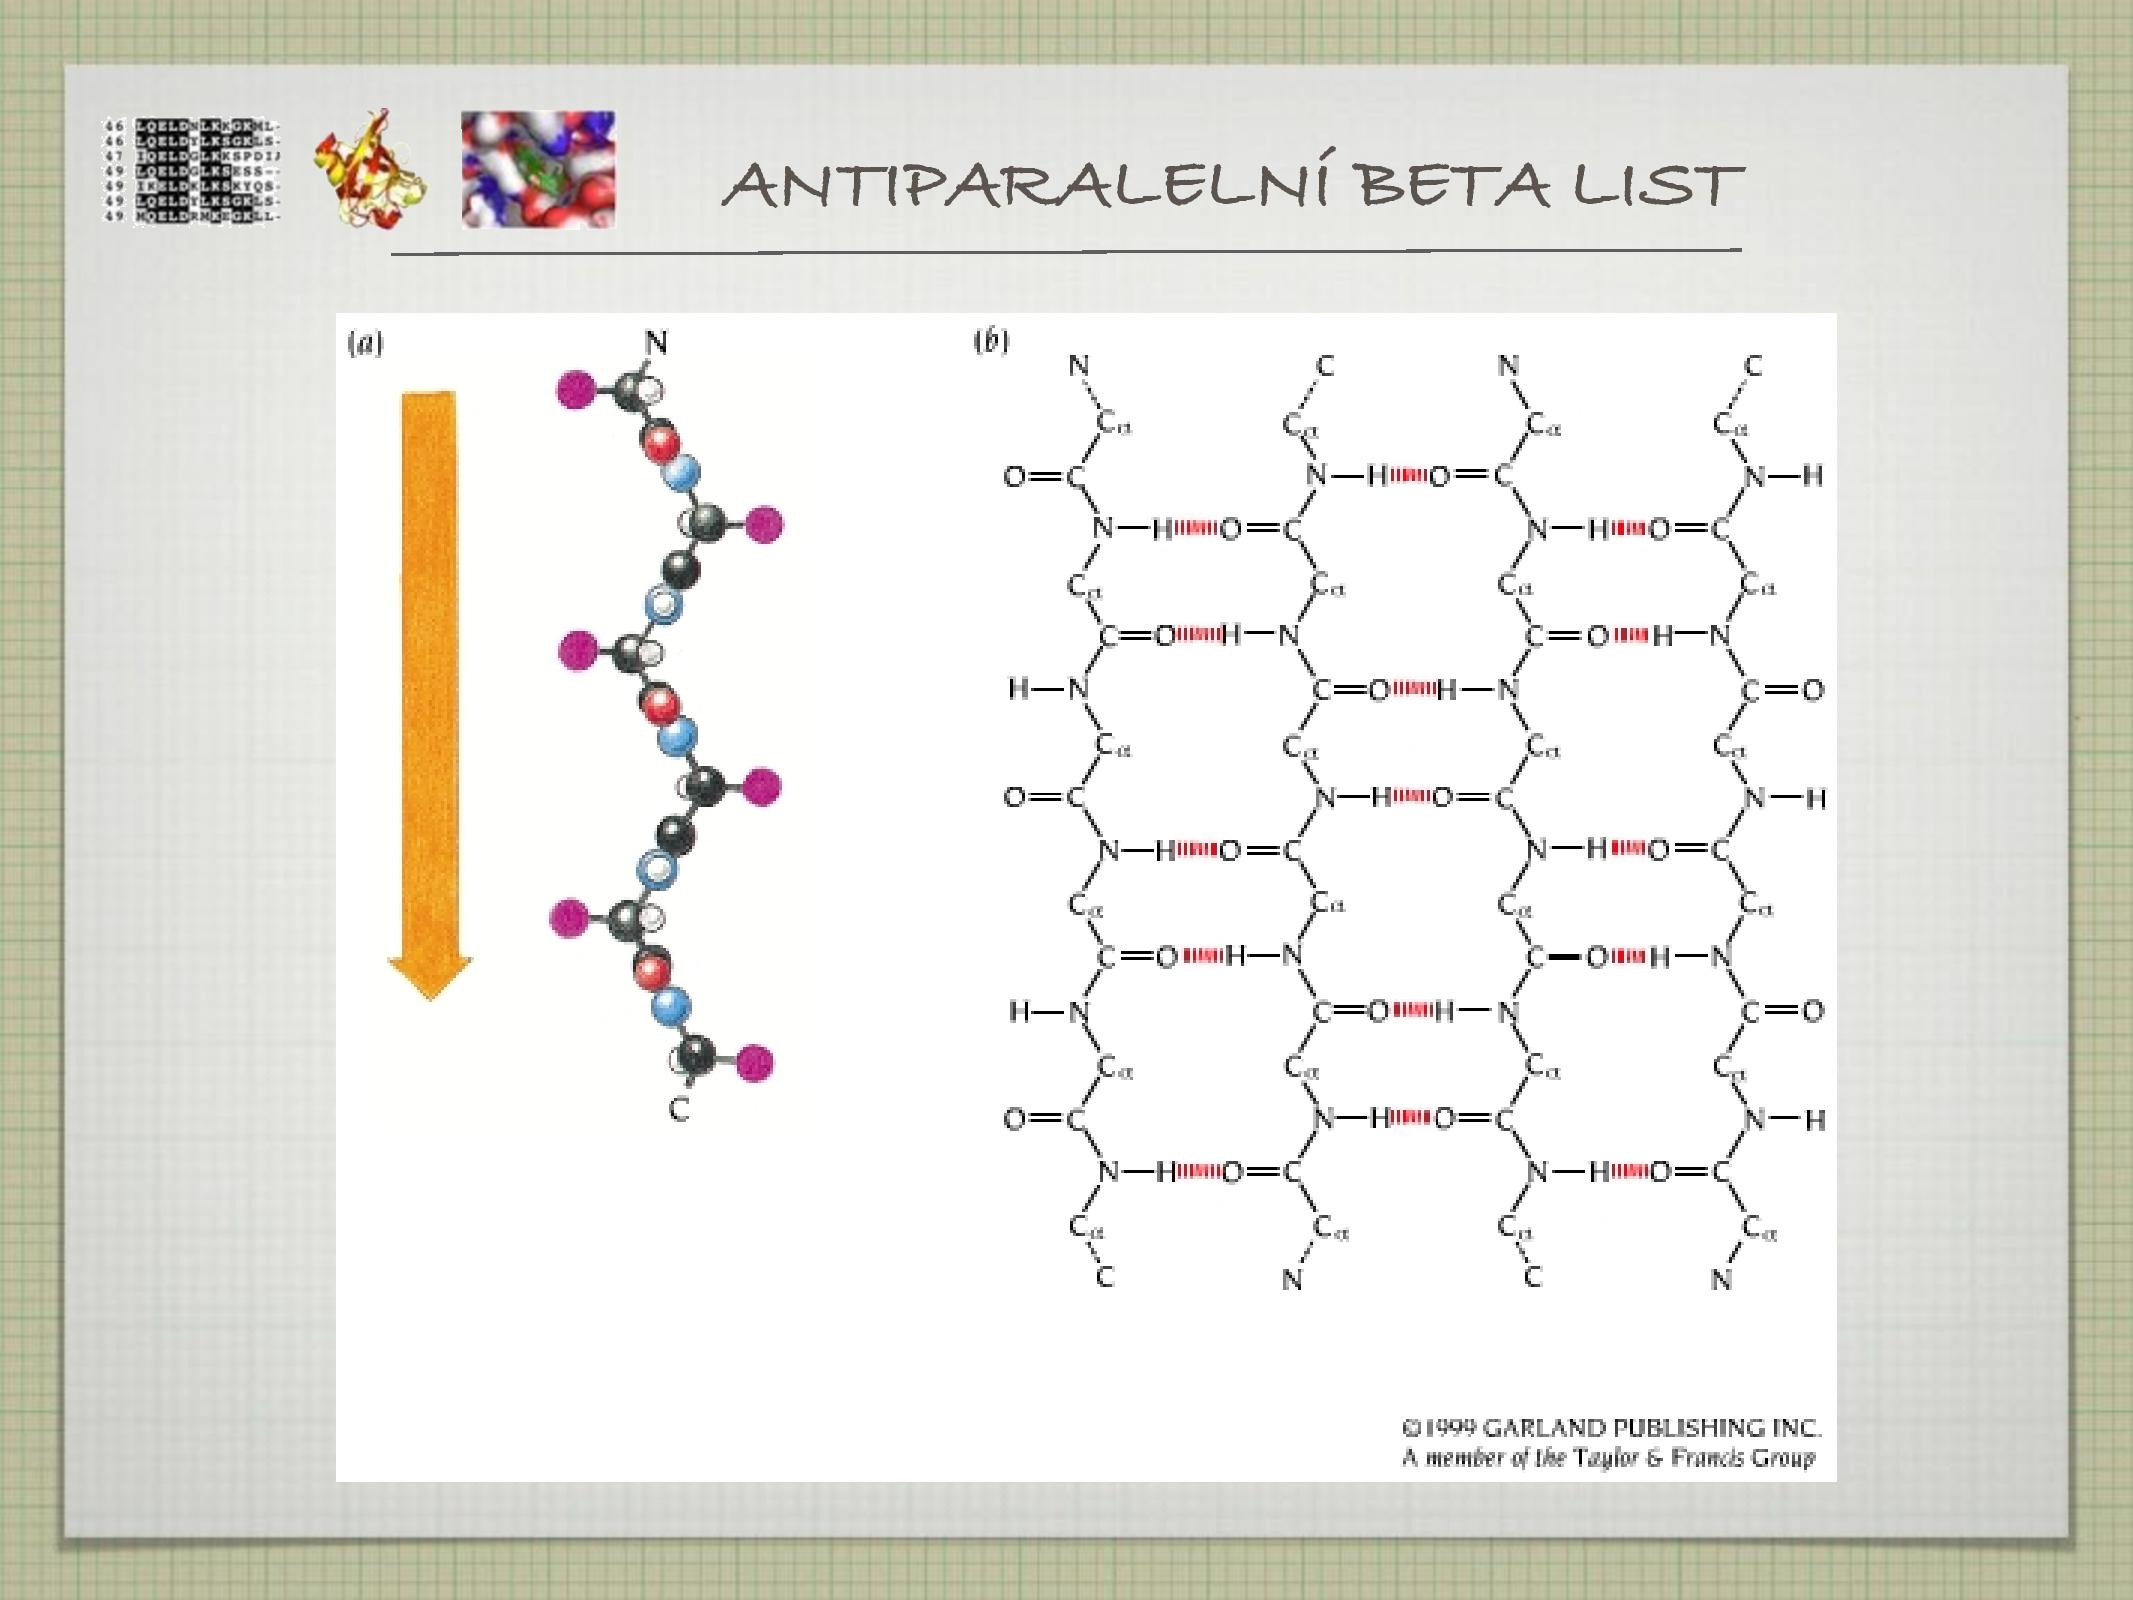
\includegraphics[width=0.85\textwidth]{slides-1/slide-63.jpg}
    \centering
    \label{slides-1-slide-63}
\end{figure}
\begin{figure}
    \caption{Prezentace č. 1, slide č. 64}
    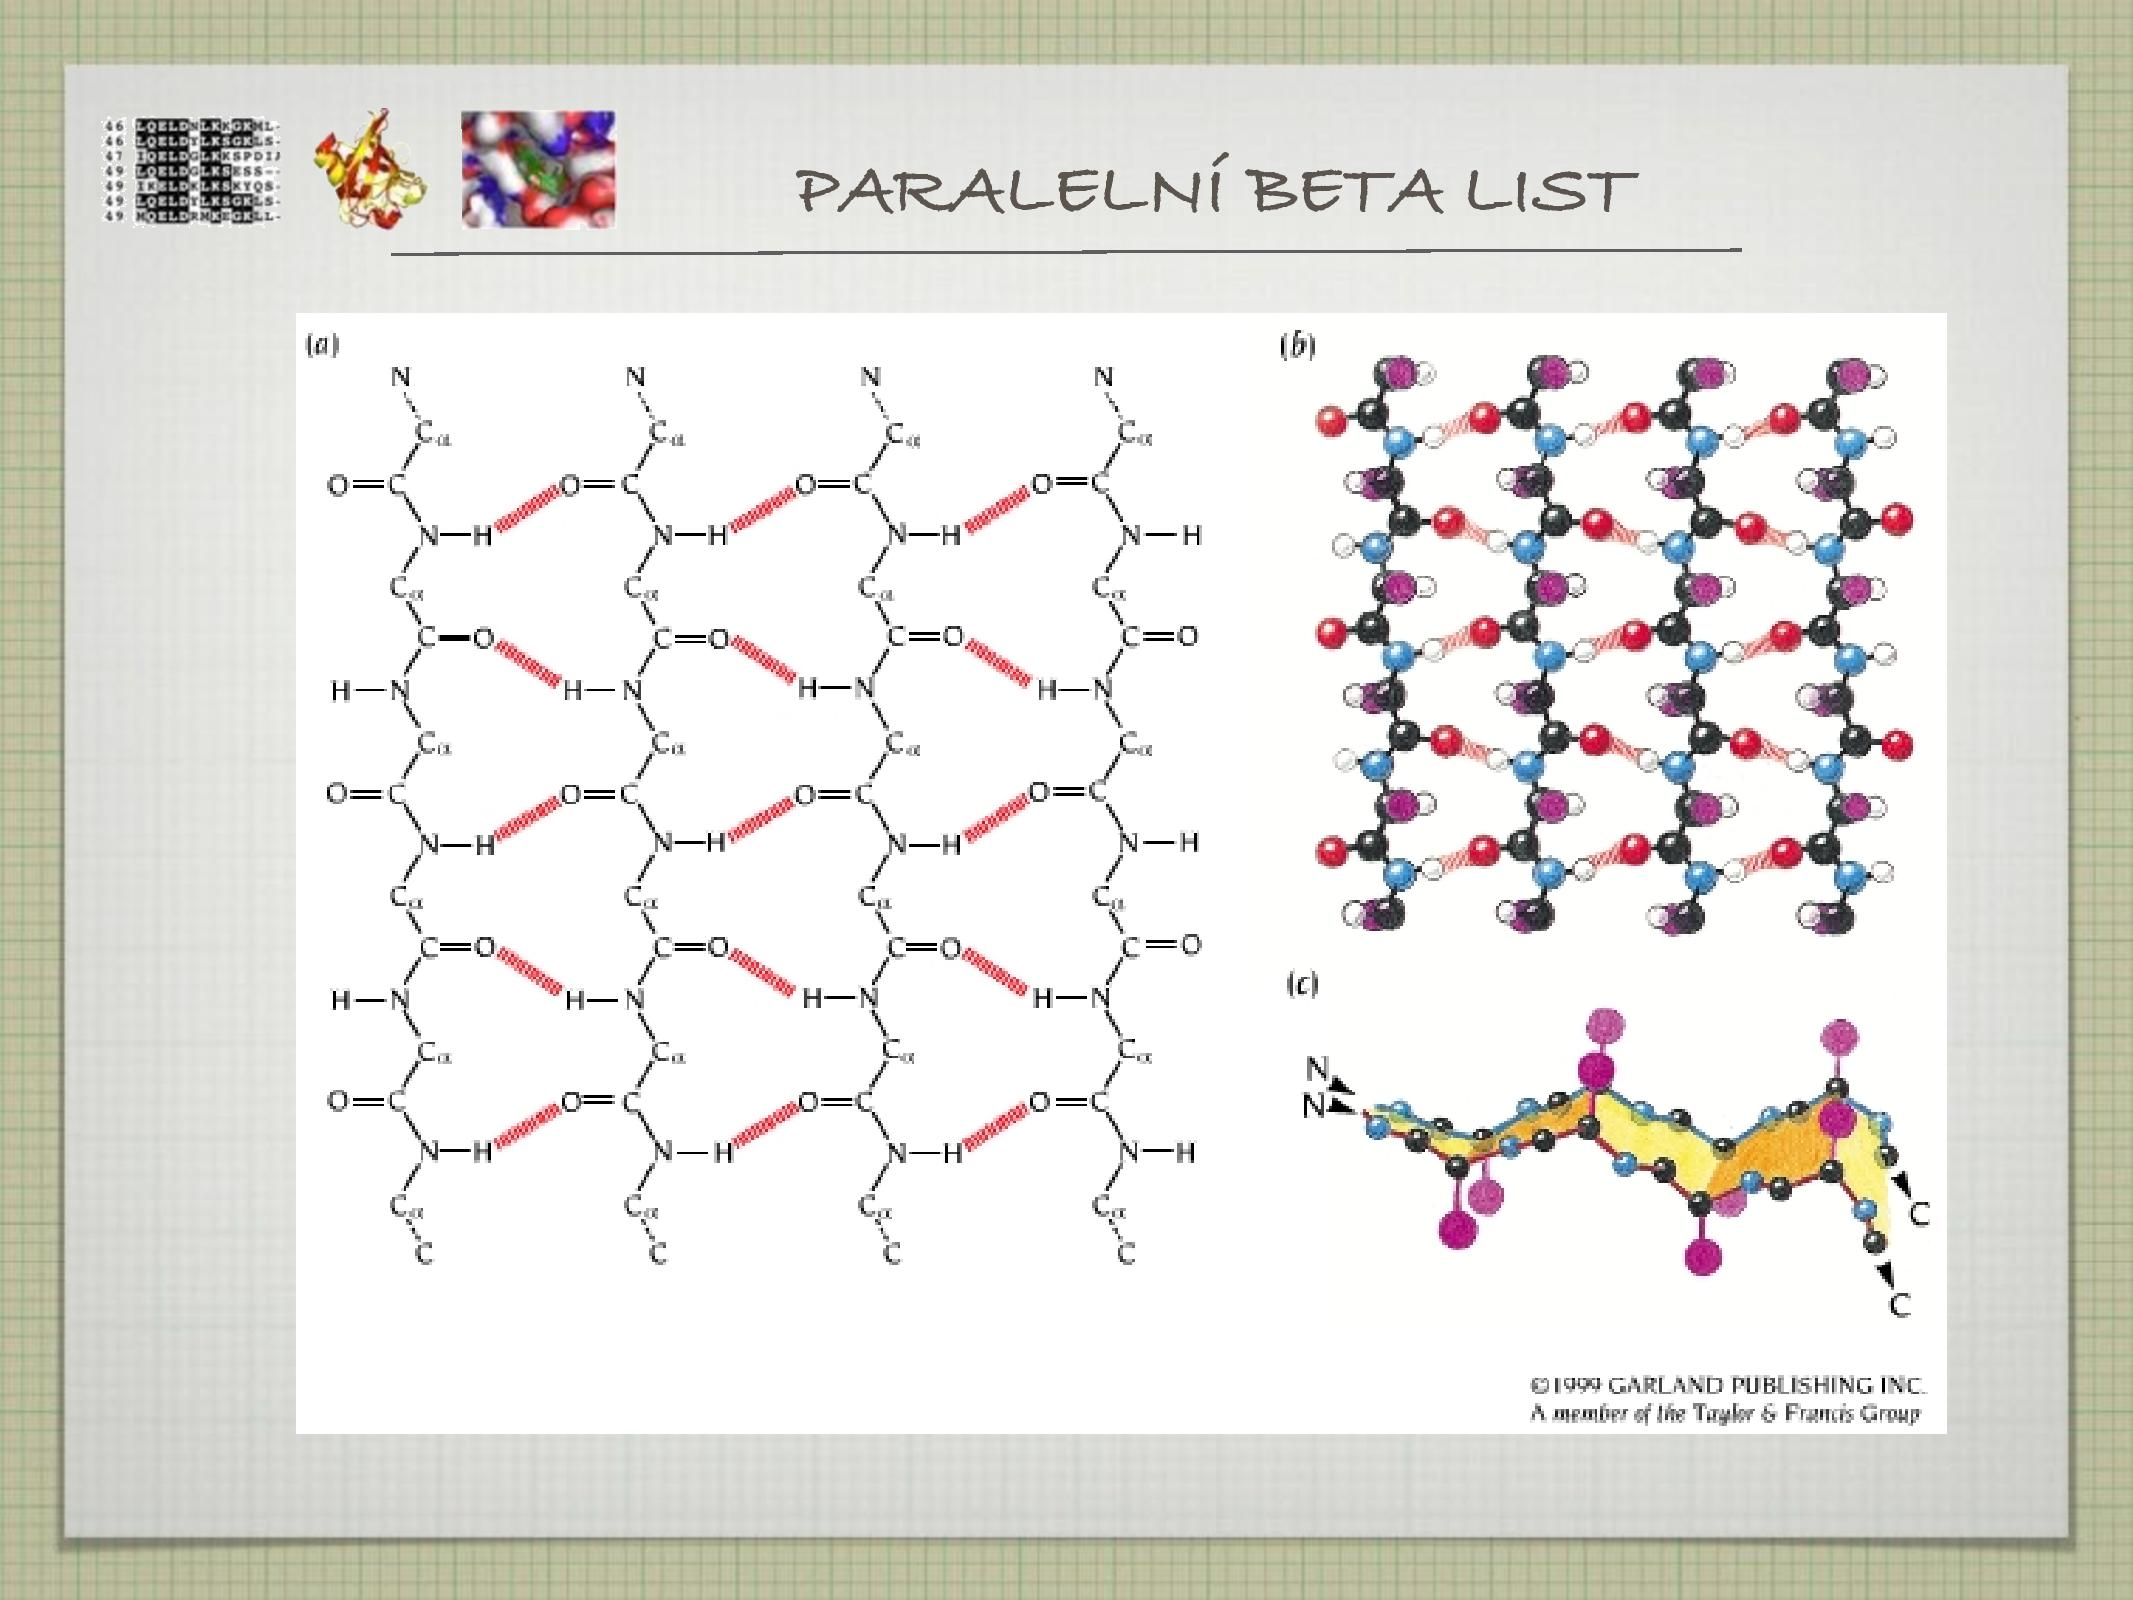
\includegraphics[width=0.85\textwidth]{slides-1/slide-64.jpg}
    \centering
    \label{slides-1-slide-64}
\end{figure}
\begin{figure}
    \caption{Prezentace č. 1, slide č. 65}
    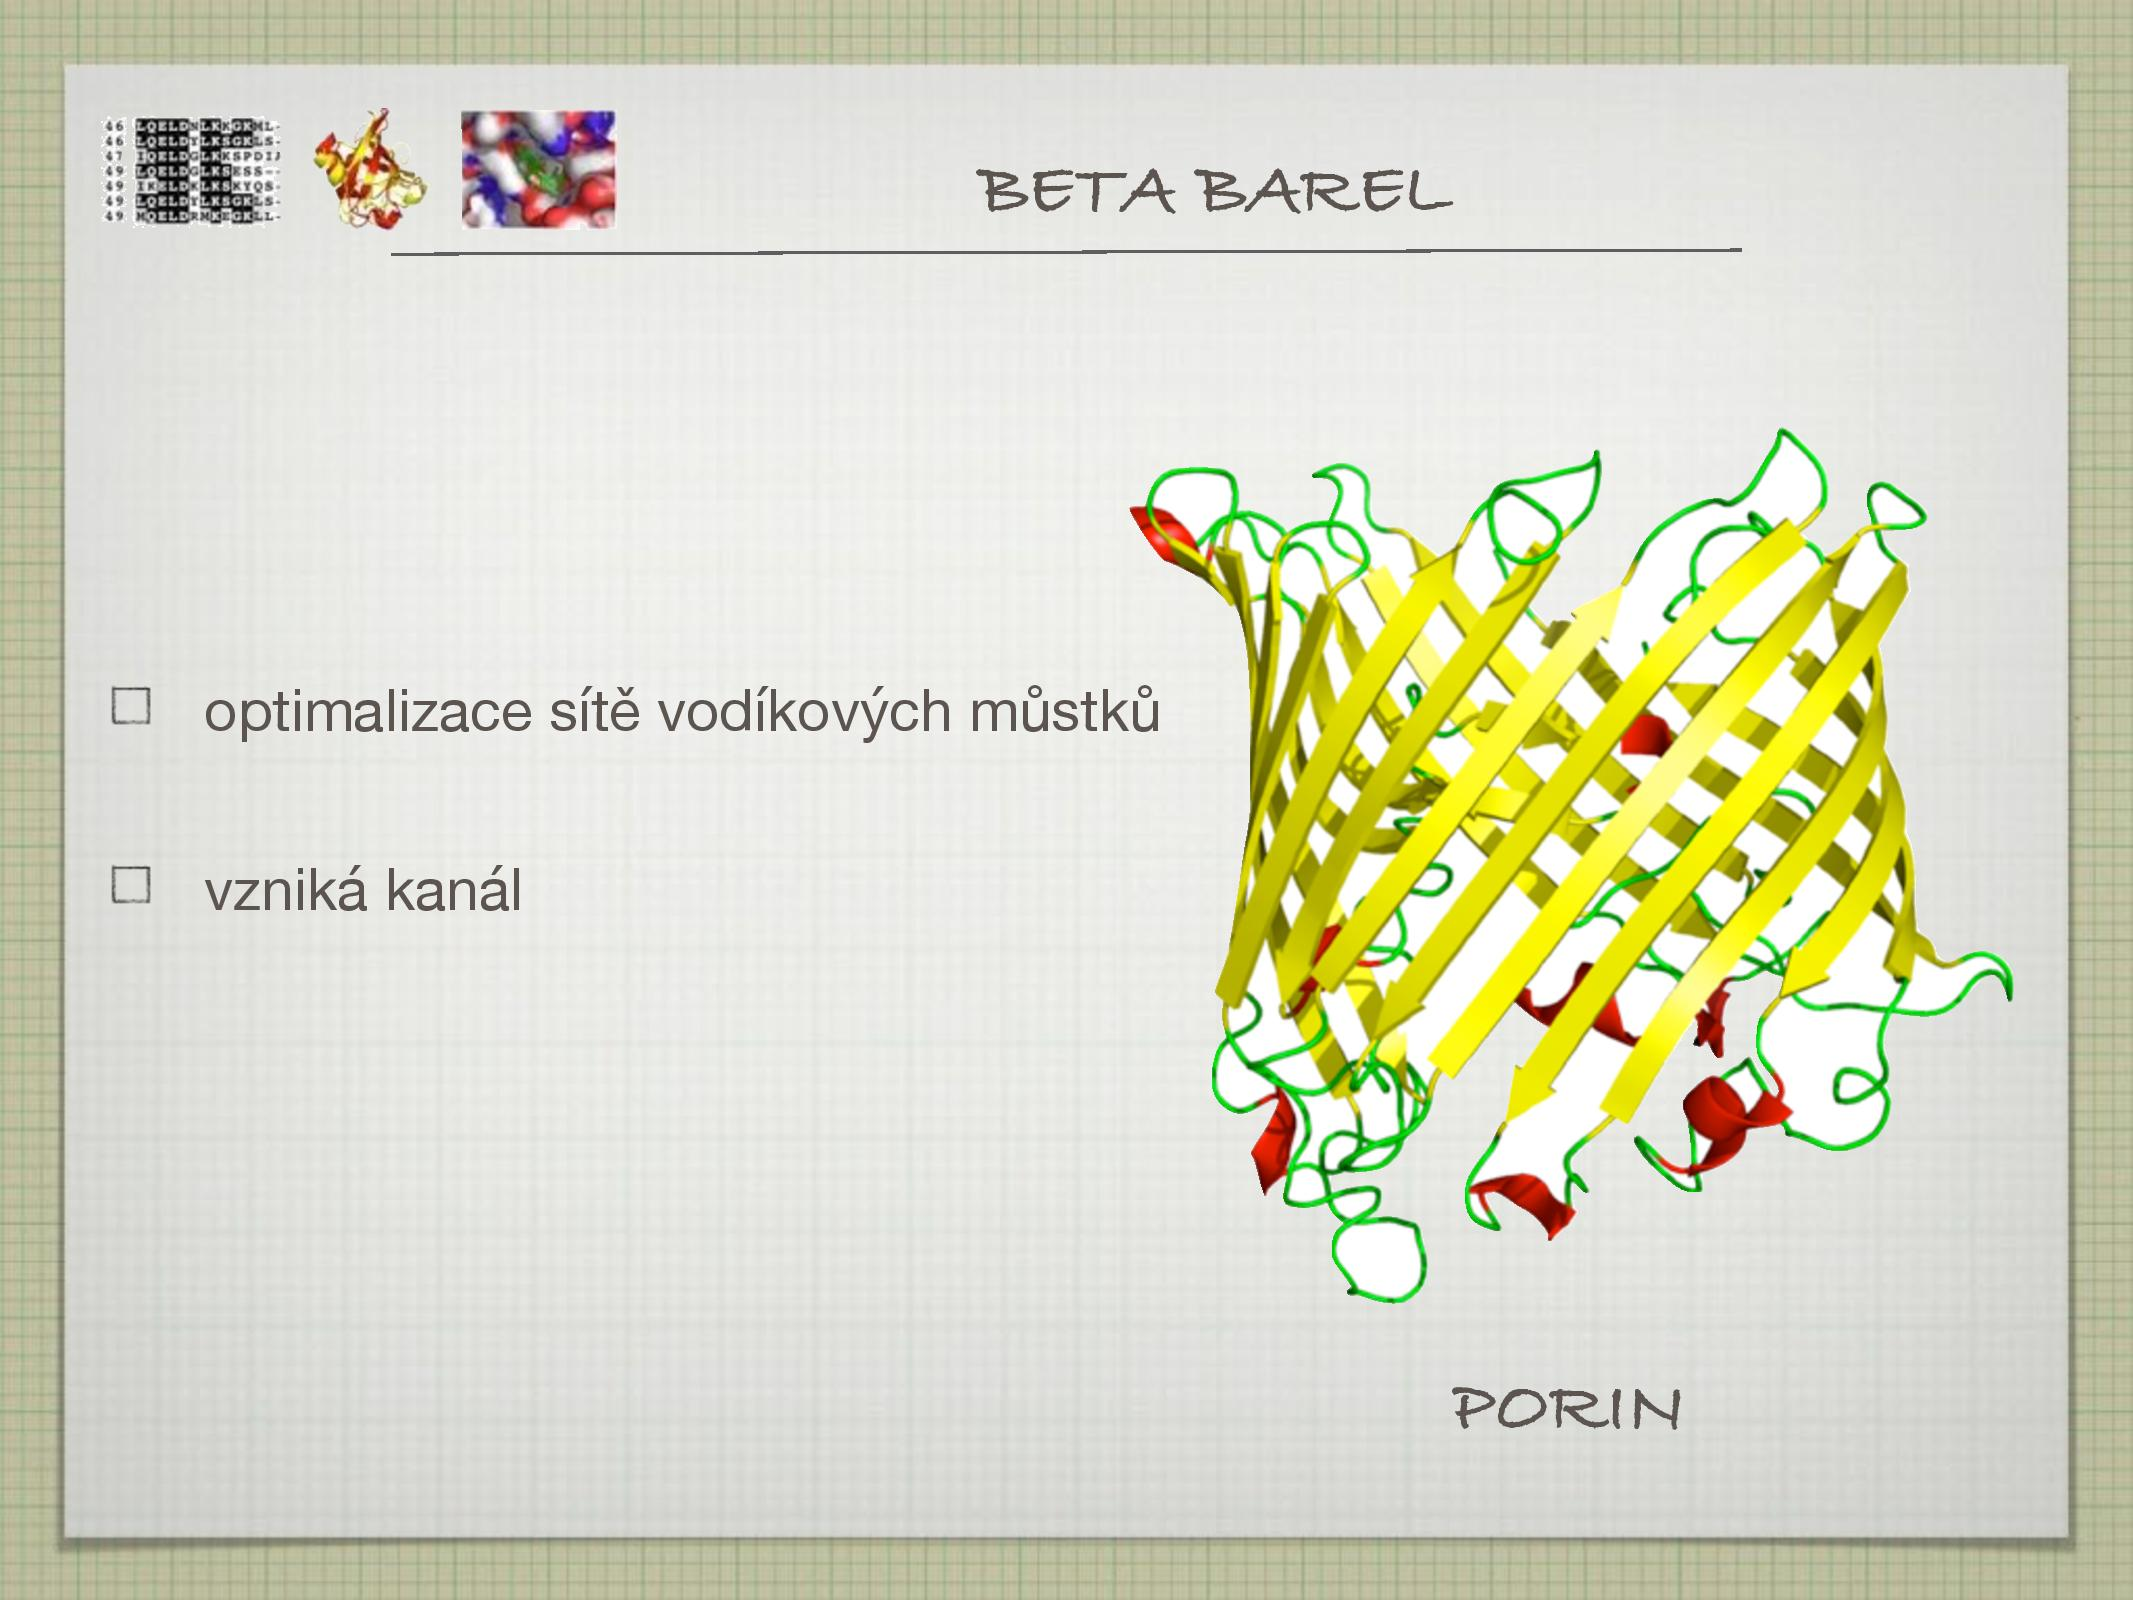
\includegraphics[width=0.85\textwidth]{slides-1/slide-65.jpg}
    \centering
    \label{slides-1-slide-65}
\end{figure}

\paragraph{Beta list}
\begin{itemize}[nosep]
    \item teoreticky jej popsal William Astbury a Linus Pauling
    \item složen z \(\beta\) hřebenů (strand)
    \item uprostřed bývají Tyr, Thr, Trp, Val a Ile, na krajích spíše Pro
    \item vzdálenost mezi \(\ce{C_\alpha}\) asi 3,5Å
    \item dvě formy
\begin{itemize}[nosep]
    \item paralelní, jsou méně stabilní (vázané atomy napříč hřebeny nejsou přesně naproti sobě)
    \item antiparalelní, jsou stabilnější, planární
\end{itemize}

    \item vznik \(\beta\) barelu
\begin{itemize}[nosep]
    \item poslední hřeben se váže na první ve stejném listu, vzniká kanál
    \item často bývá stočený
    \item často v membránách
\end{itemize}

\end{itemize}



\begin{figure}
    \caption{Prezentace č. 1, slide č. 66}
    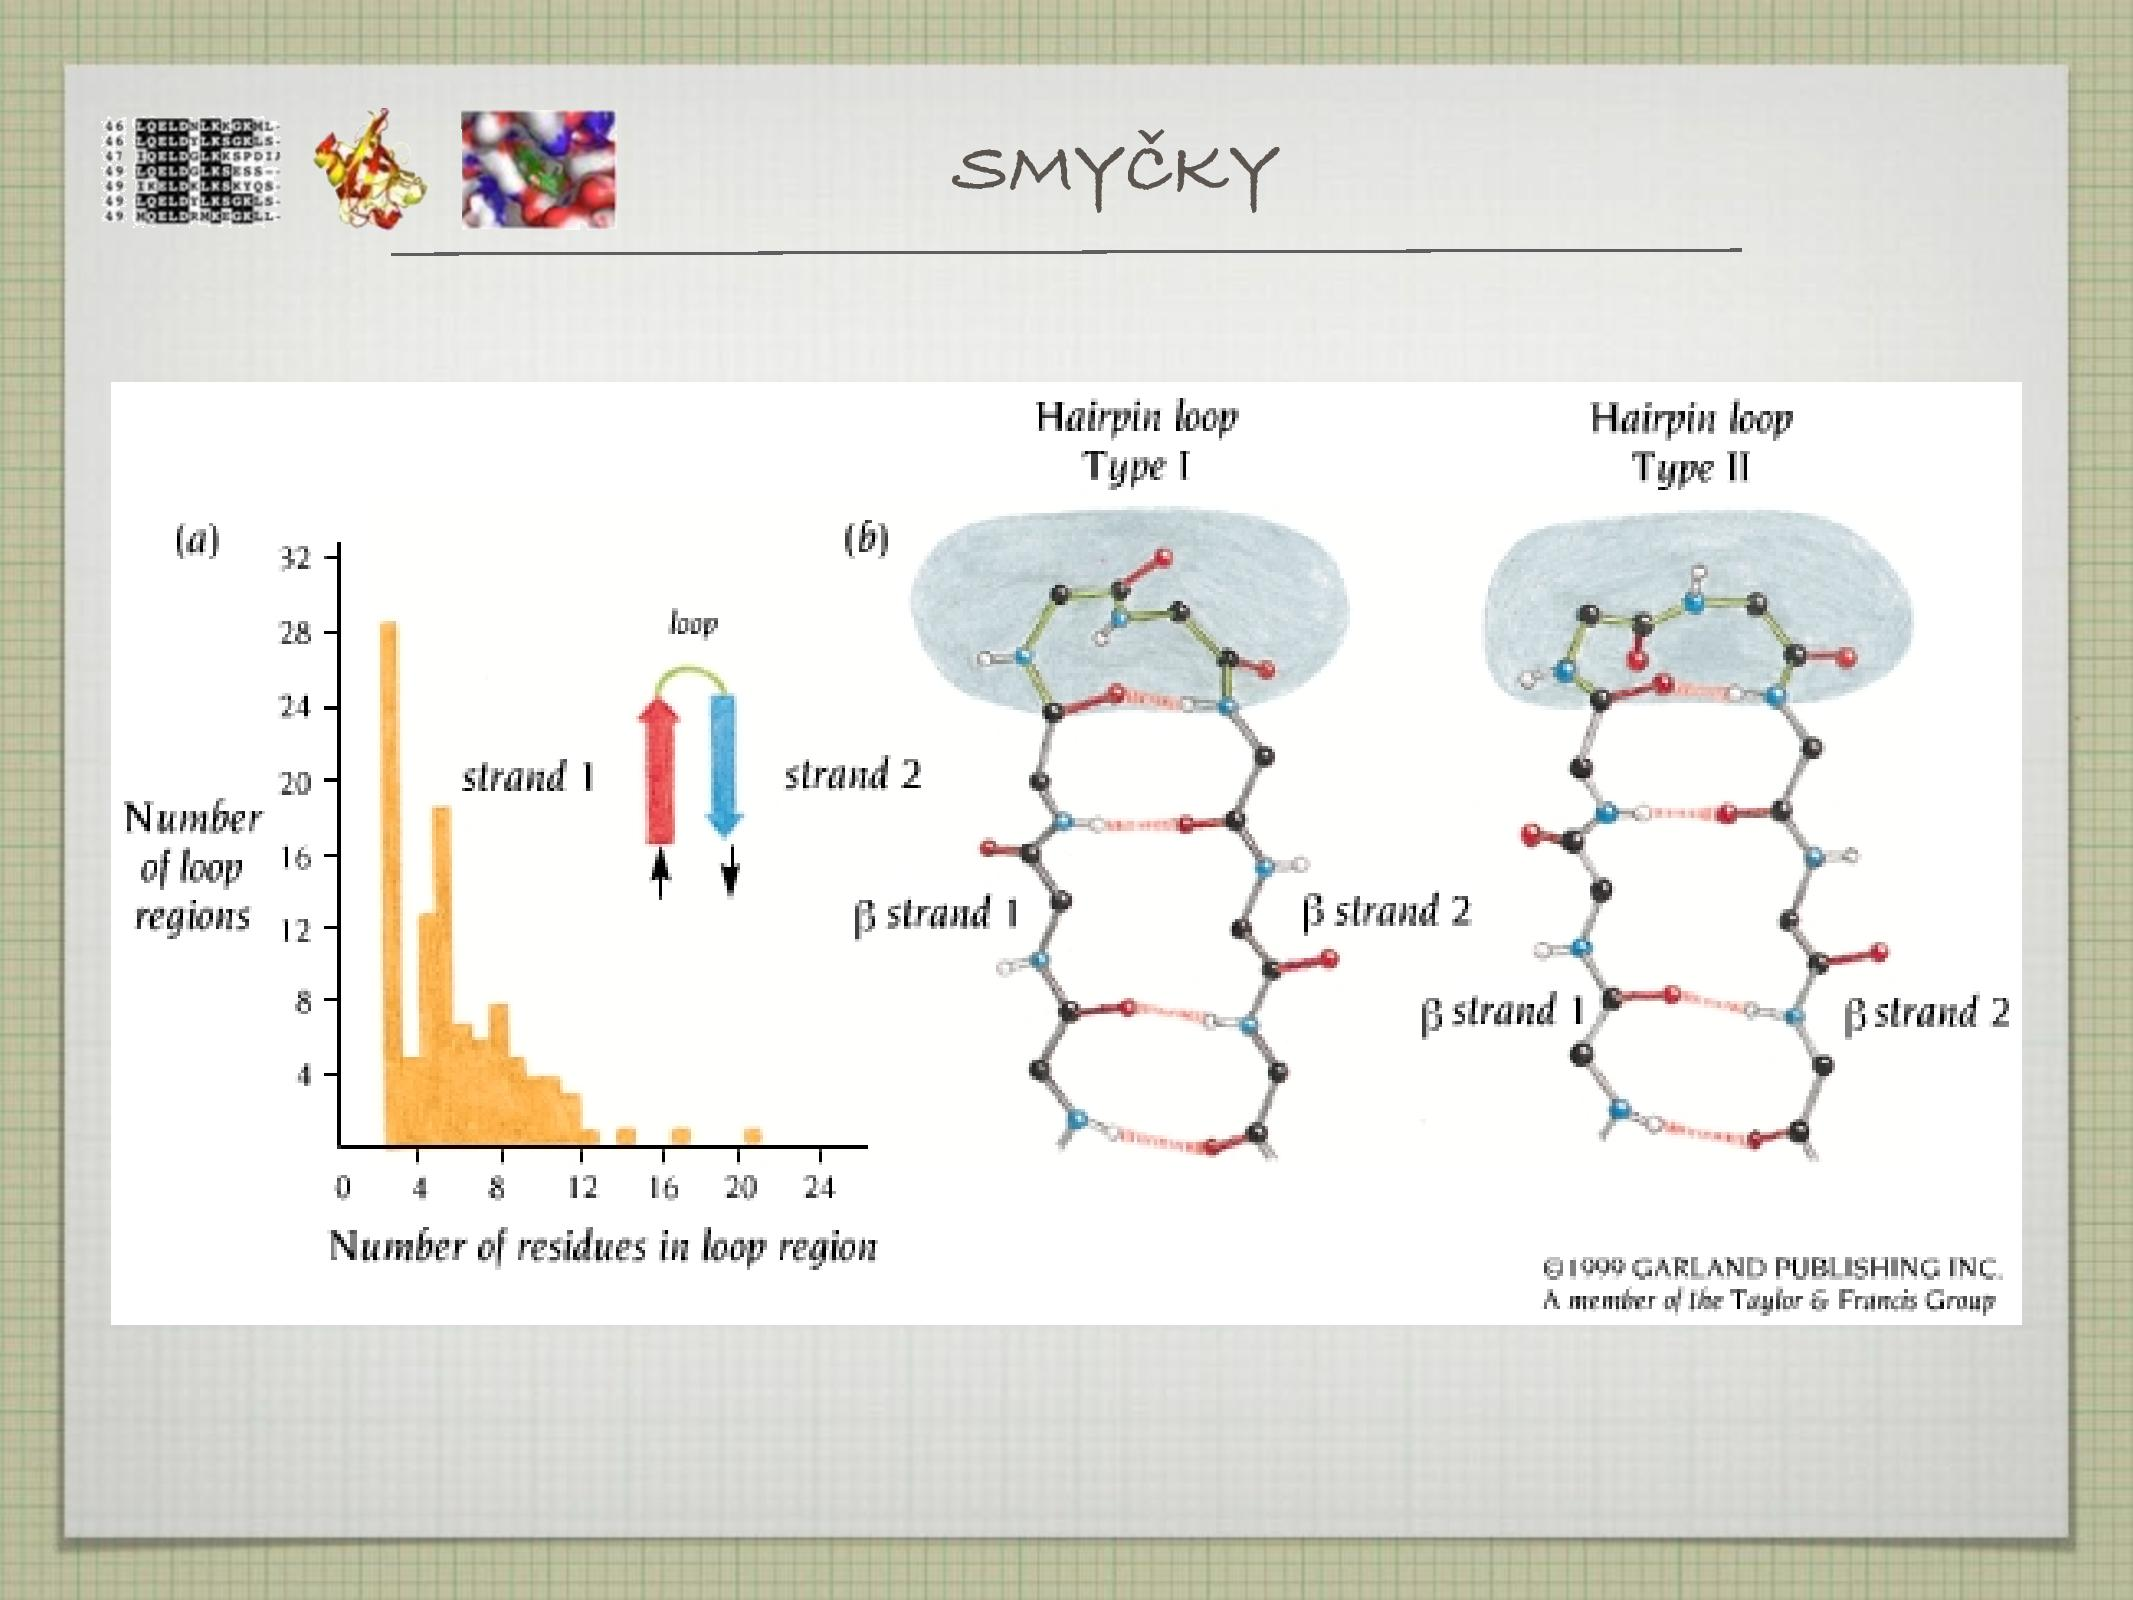
\includegraphics[width=0.85\textwidth]{slides-1/slide-66.jpg}
    \centering
    \label{slides-1-slide-66}
\end{figure}

\paragraph{Smyčky}
\begin{itemize}[nosep]
    \item nepravidelné struktury
    \item často hodně Gly (protože je malý)
    \item spojují helixy a listy
    \item bývají krátké, většinou kolem 4,5 AK
    \item existuje více druhů (vlásenky, loopy, atd.)
\end{itemize}



\begin{figure}
    \caption{Prezentace č. 1, slide č. 67}
    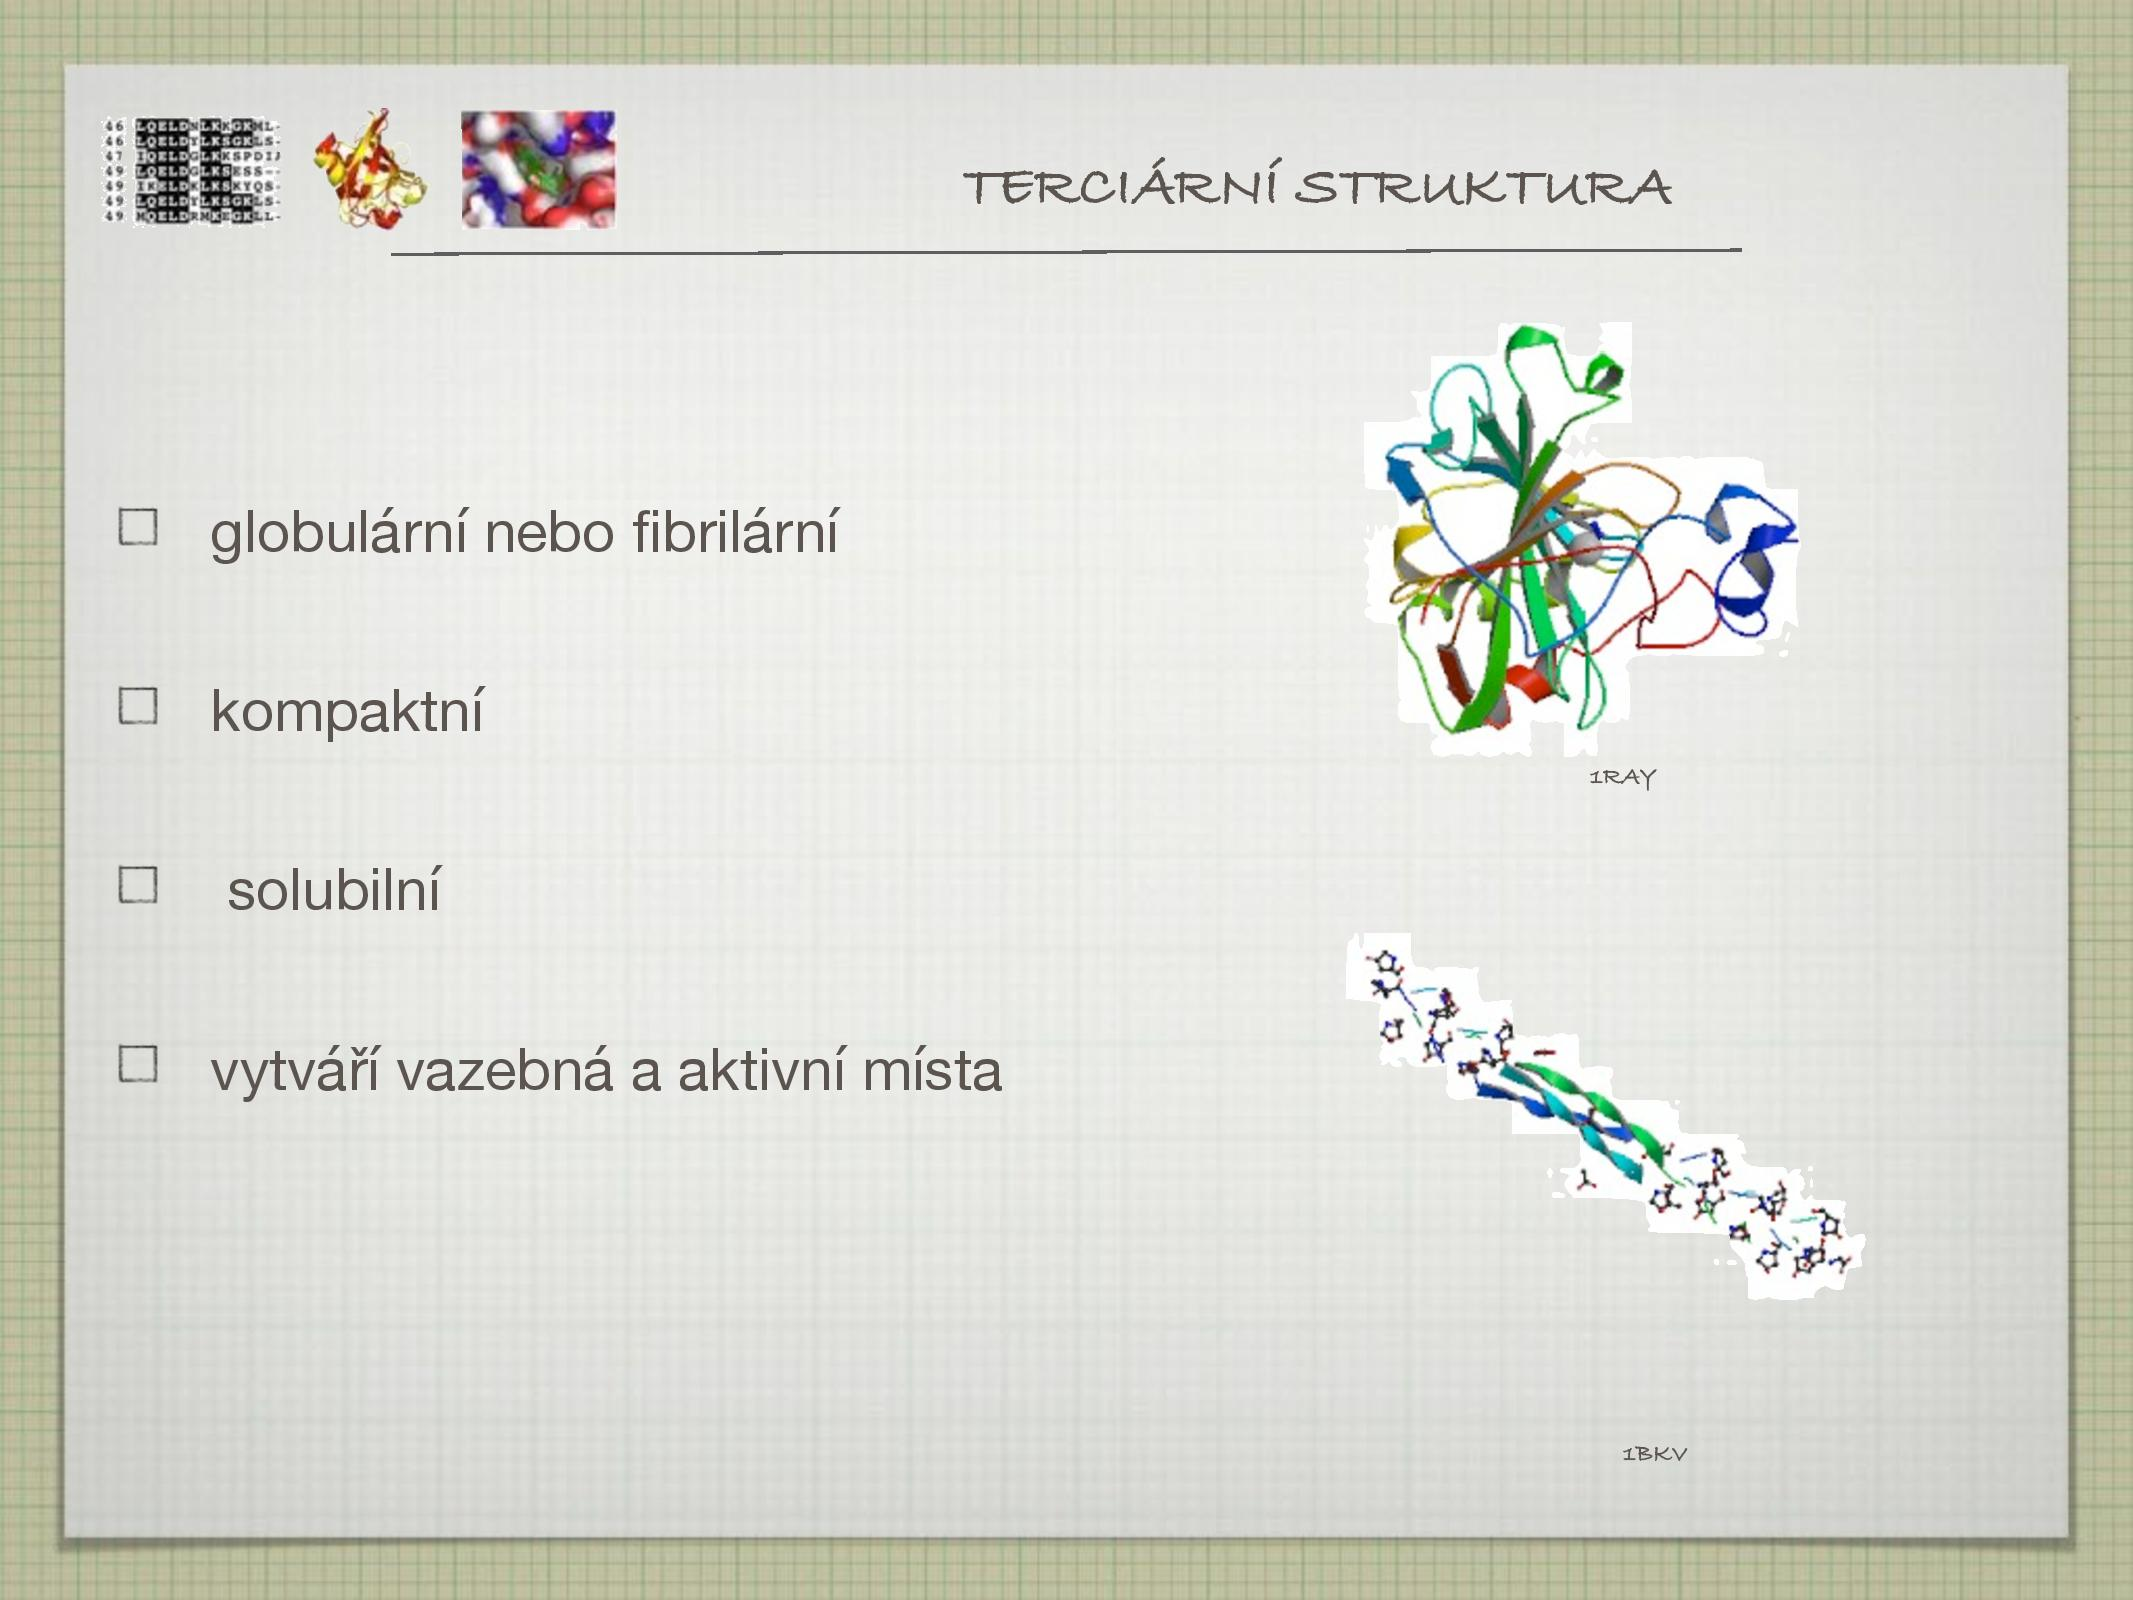
\includegraphics[width=0.85\textwidth]{slides-1/slide-67.jpg}
    \centering
    \label{slides-1-slide-67}
\end{figure}

\paragraph{Terciární struktura proteinu}
\begin{itemize}[nosep]
    \item někdy také \emph{konformace}, \emph{topologie} nebo \emph{folding}
    \item celková 3D struktura proteinu
    \item dva typy
\begin{itemize}[nosep]
    \item globulární, nepříliš uspořádaná
    \item fibrilární, uspořádaná do vláken
\end{itemize}

    \item rozhoduje o solubilitě
    \item vytváří vazebná a antivazebná místa
\end{itemize}



\begin{figure}
    \caption{Prezentace č. 1, slide č. 68}
    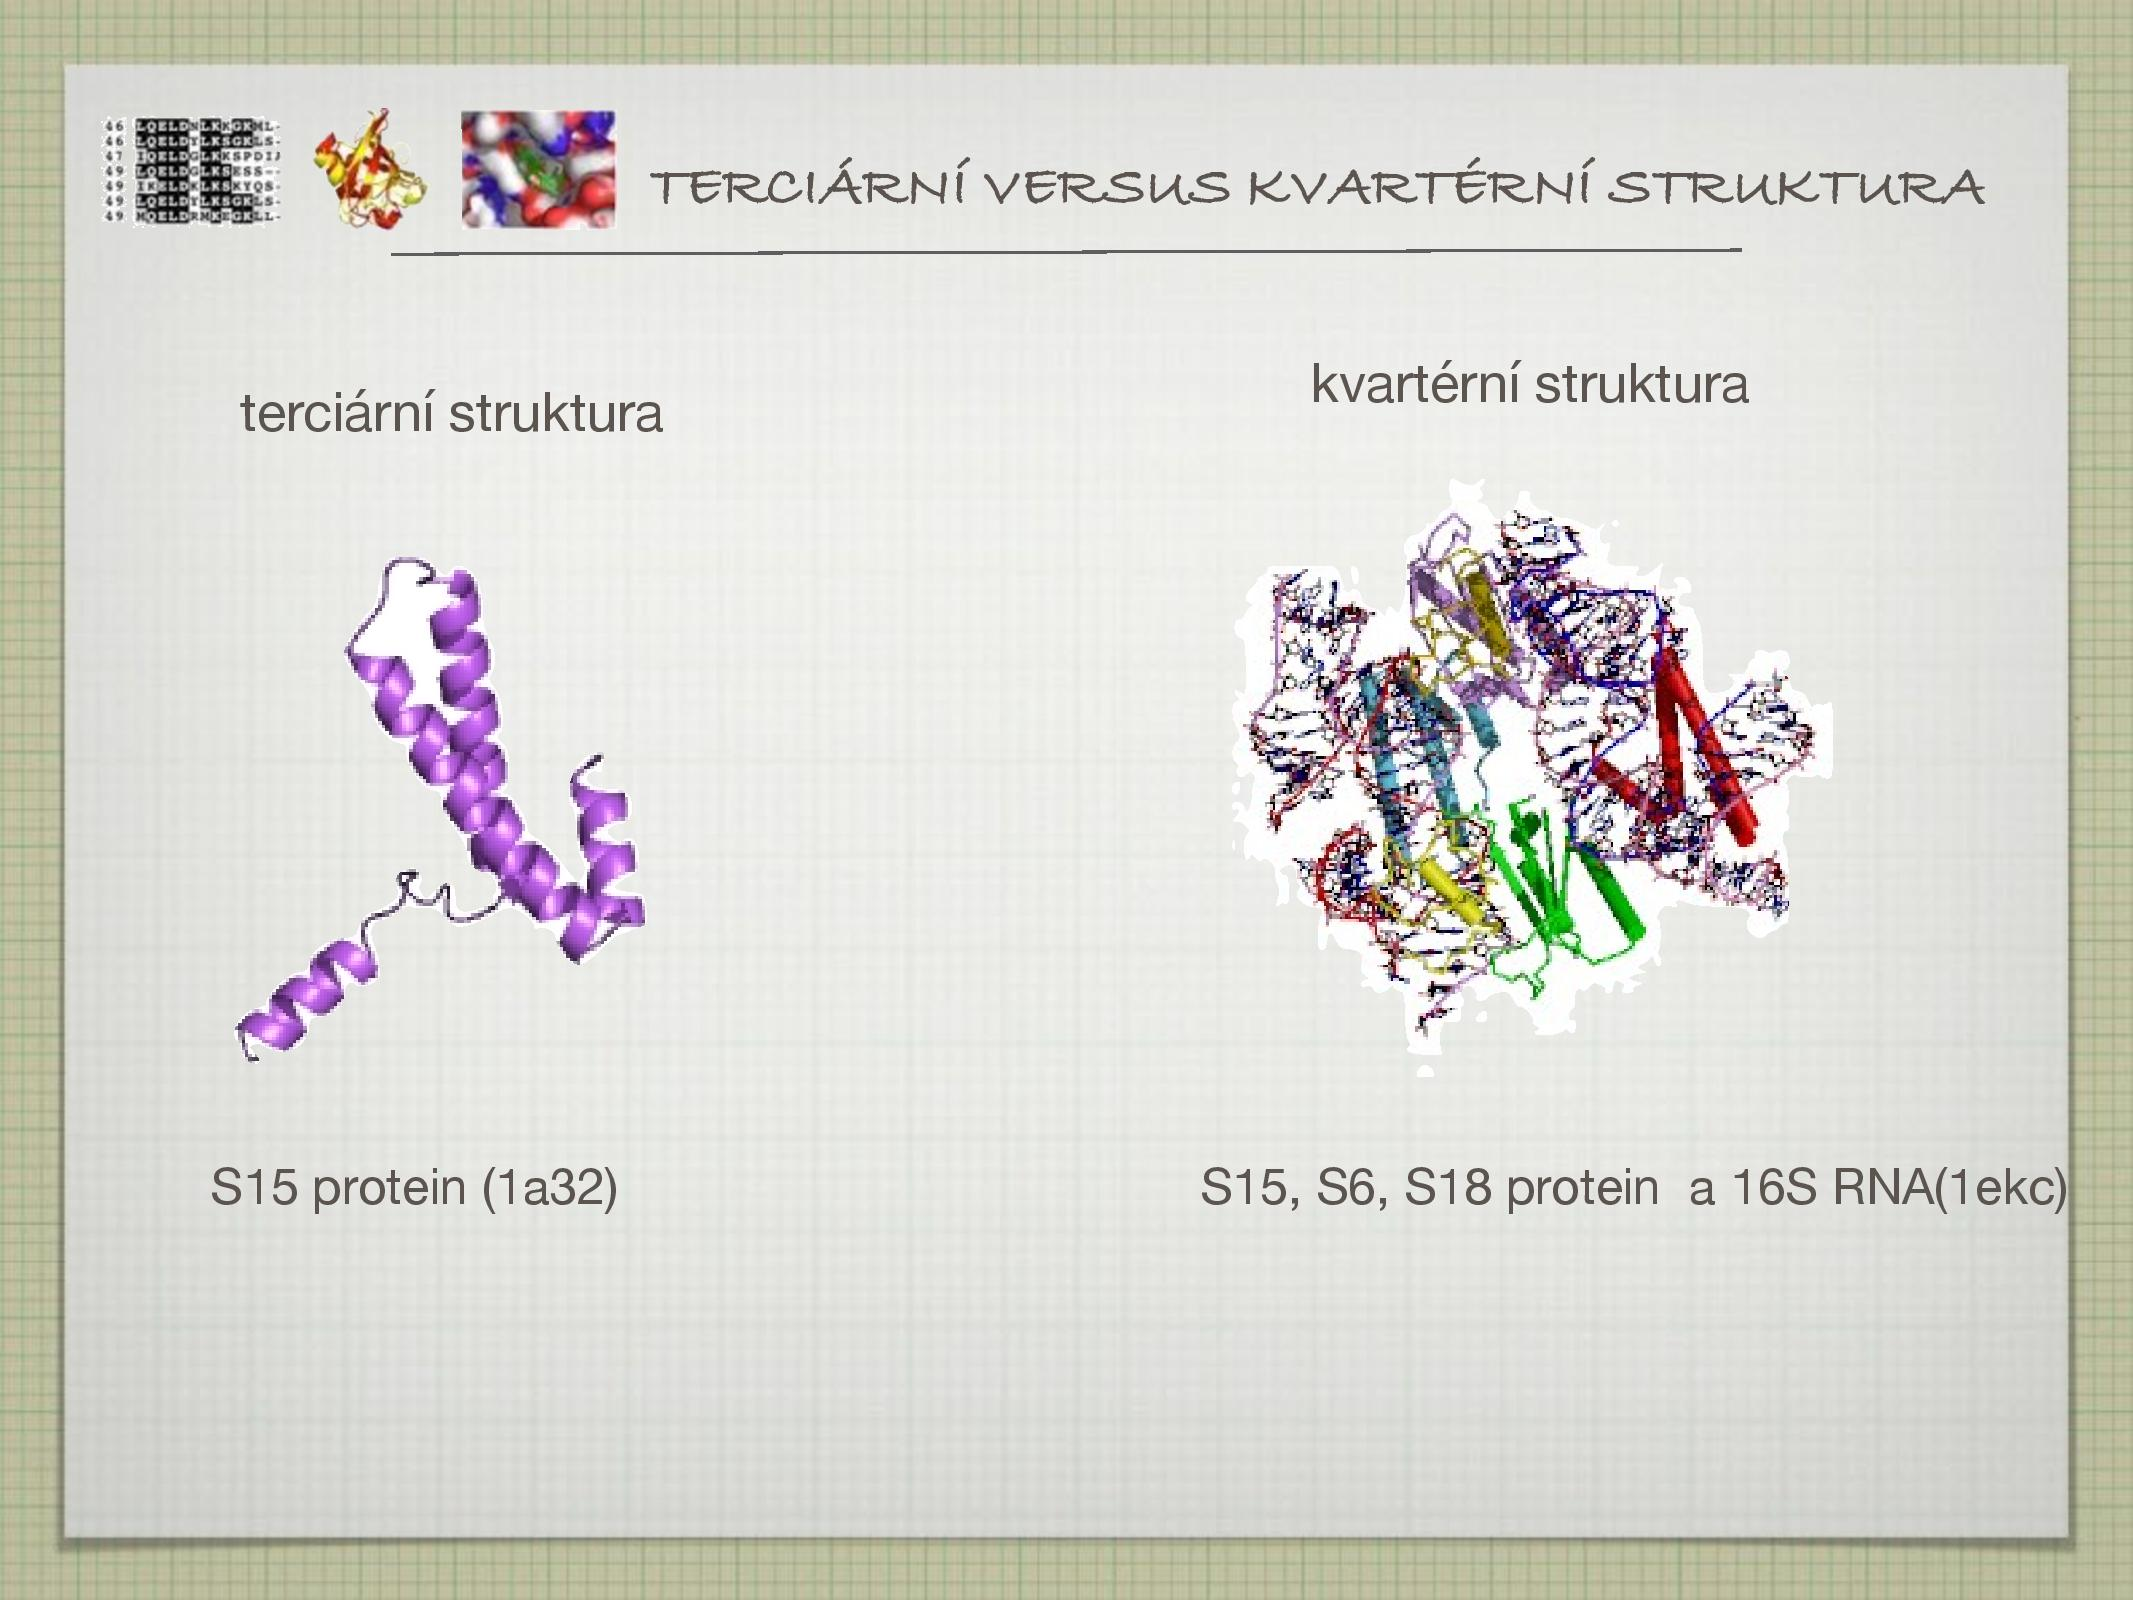
\includegraphics[width=0.85\textwidth]{slides-1/slide-68.jpg}
    \centering
    \label{slides-1-slide-68}
\end{figure}

Kvarterní struktura proteinu popsiuje uspořádání několika terciárních struktur (například v dimerech).

\chapter{Sequence alignment} \label{Sequence alignment}

\marginline{Přednáška č. 4}

Základní bioinformatická metoda užíváná k porovnání dvou sekvencí (DNA, proteinů). Obecně se jedná o nějaké seřazení sekvencí pod sebe. Dobrý alignment dvou sekvencí má však důležitou vlastnost: pod sebou jsou jednotky (nukleotidy, AK), které se vyvinuly ze stejného předka. Někdy byly určité jednotky v průběhu evoluce přidány nebo odebrány, což se v rámci alignmentu značí pomlčkami (viz níže).

Než se dostaneme k samotnému procesu alignmentu (tj. zjišťování, které jednotky a potažmo celé sekvence jsou evolučně spřízněné), ukážeme několik jeho praktických využití.

\begin{figure}
    \caption{Prezentace č. 2, slide č. 26}
    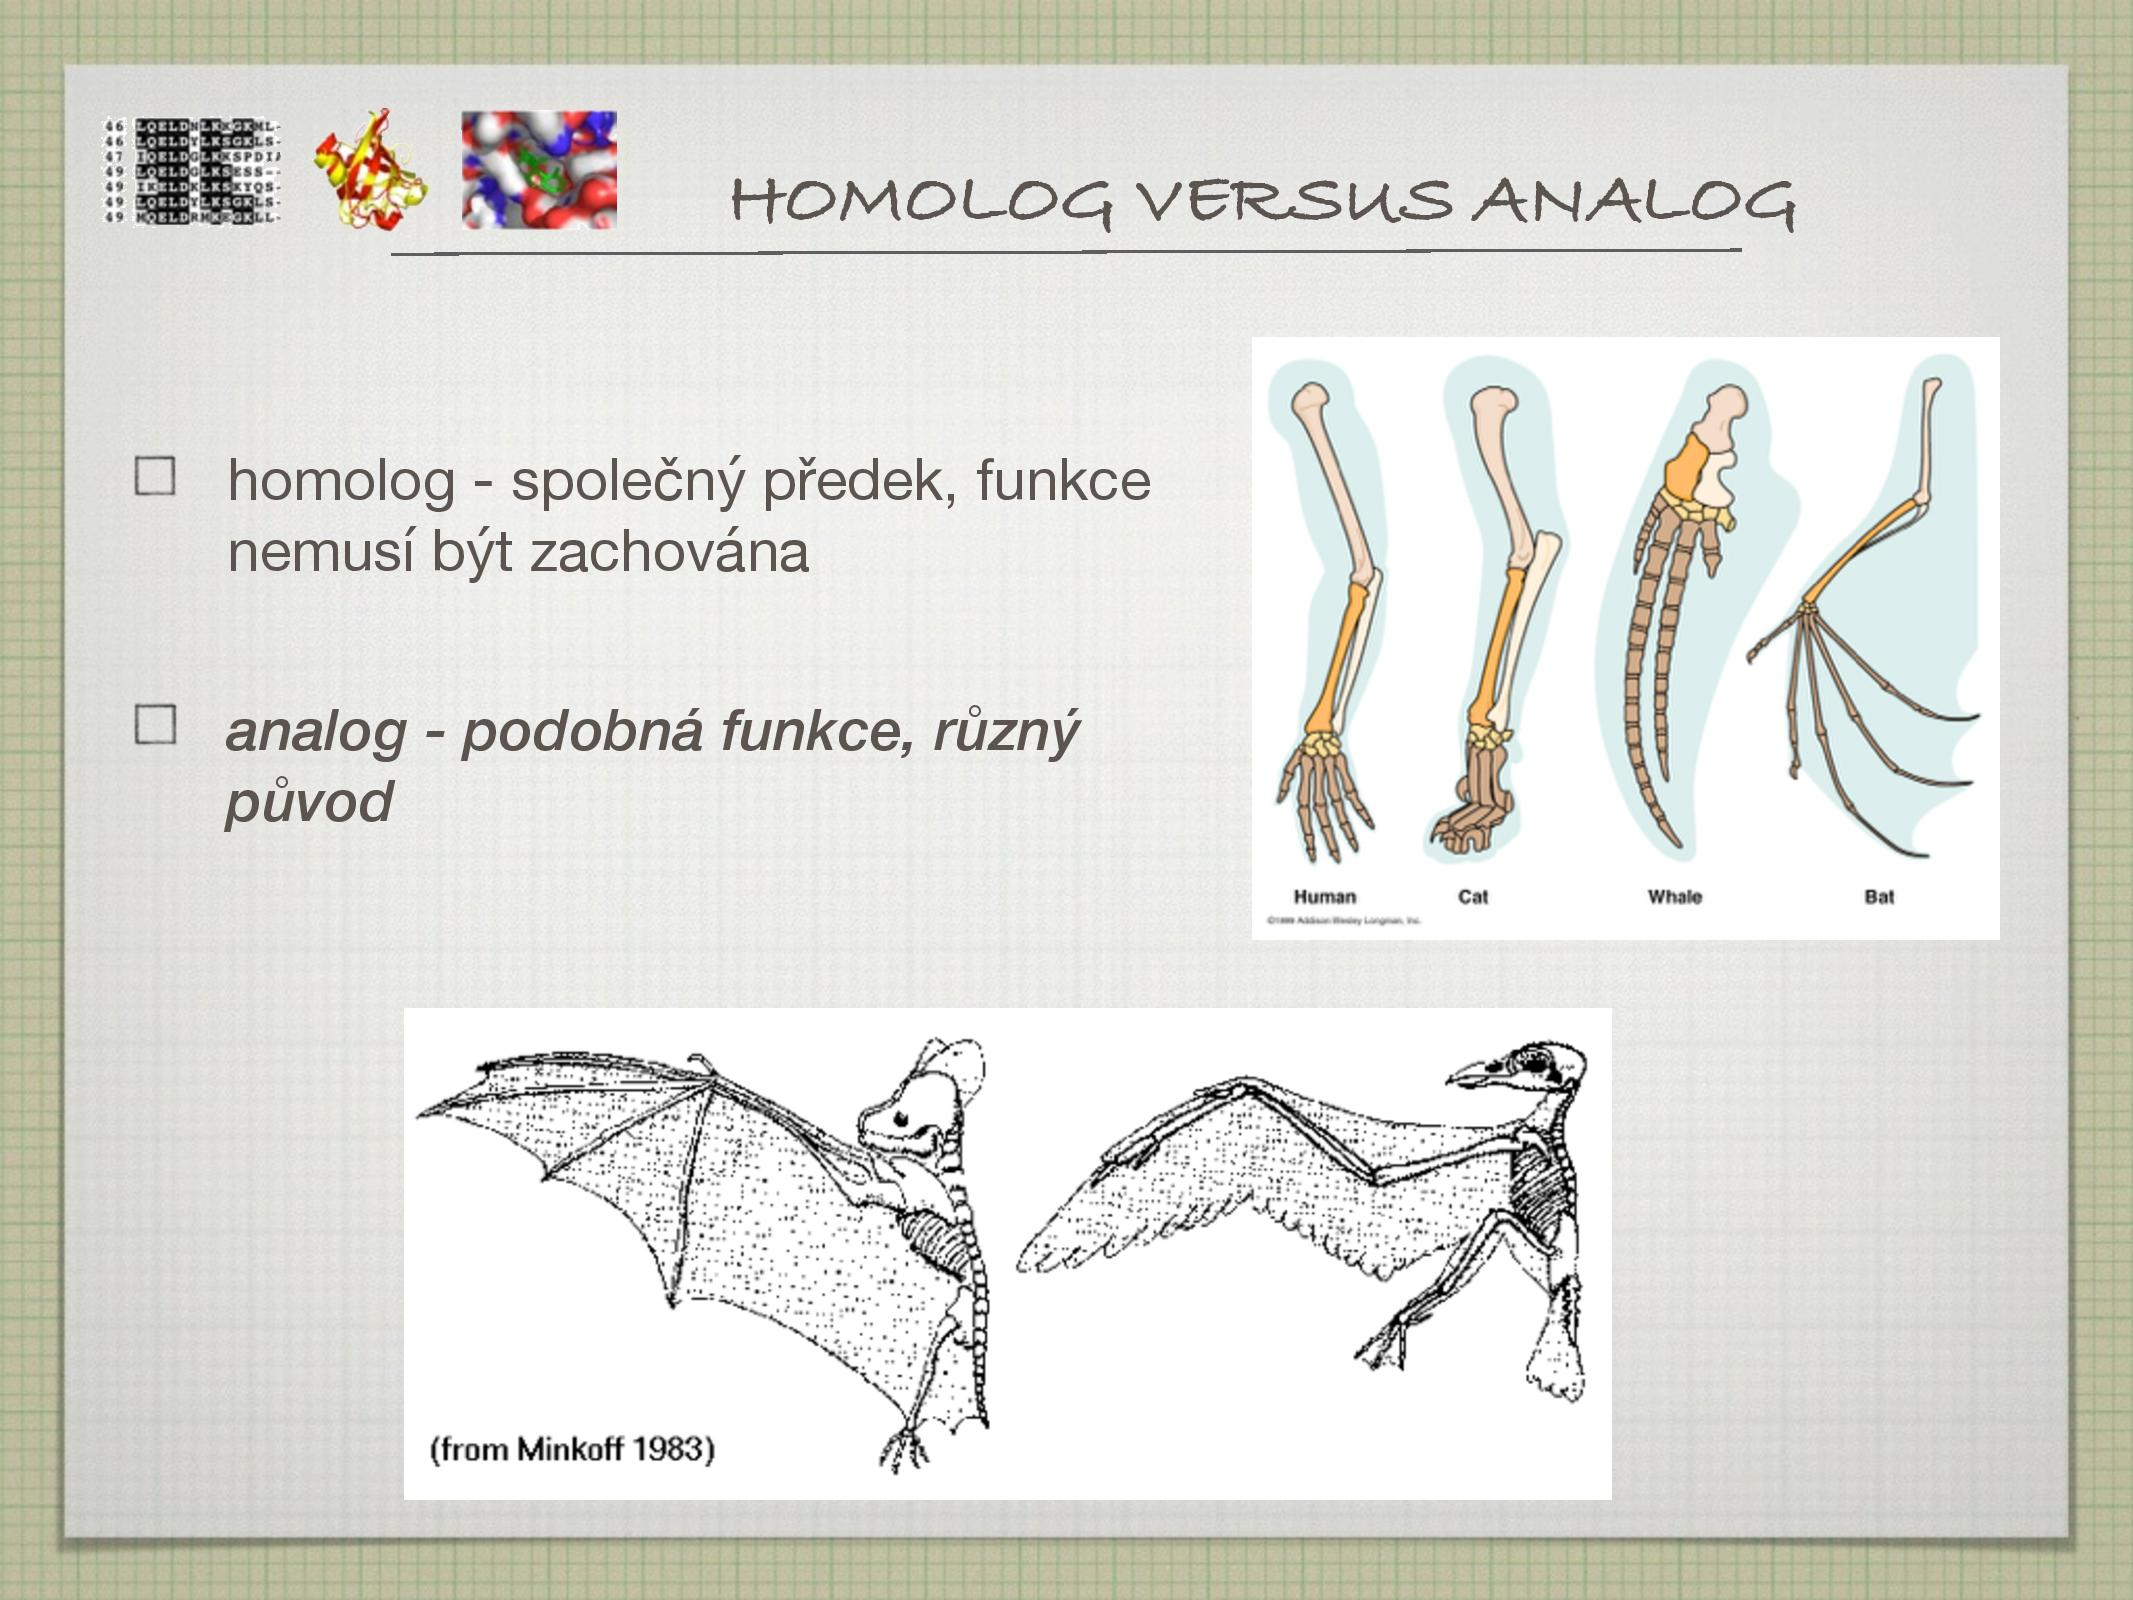
\includegraphics[width=0.85\textwidth]{slides-2/slide-26.jpg}
    \centering
    \label{slides-2-slide-26}
\end{figure}
\begin{figure}
    \caption{Prezentace č. 2, slide č. 27}
    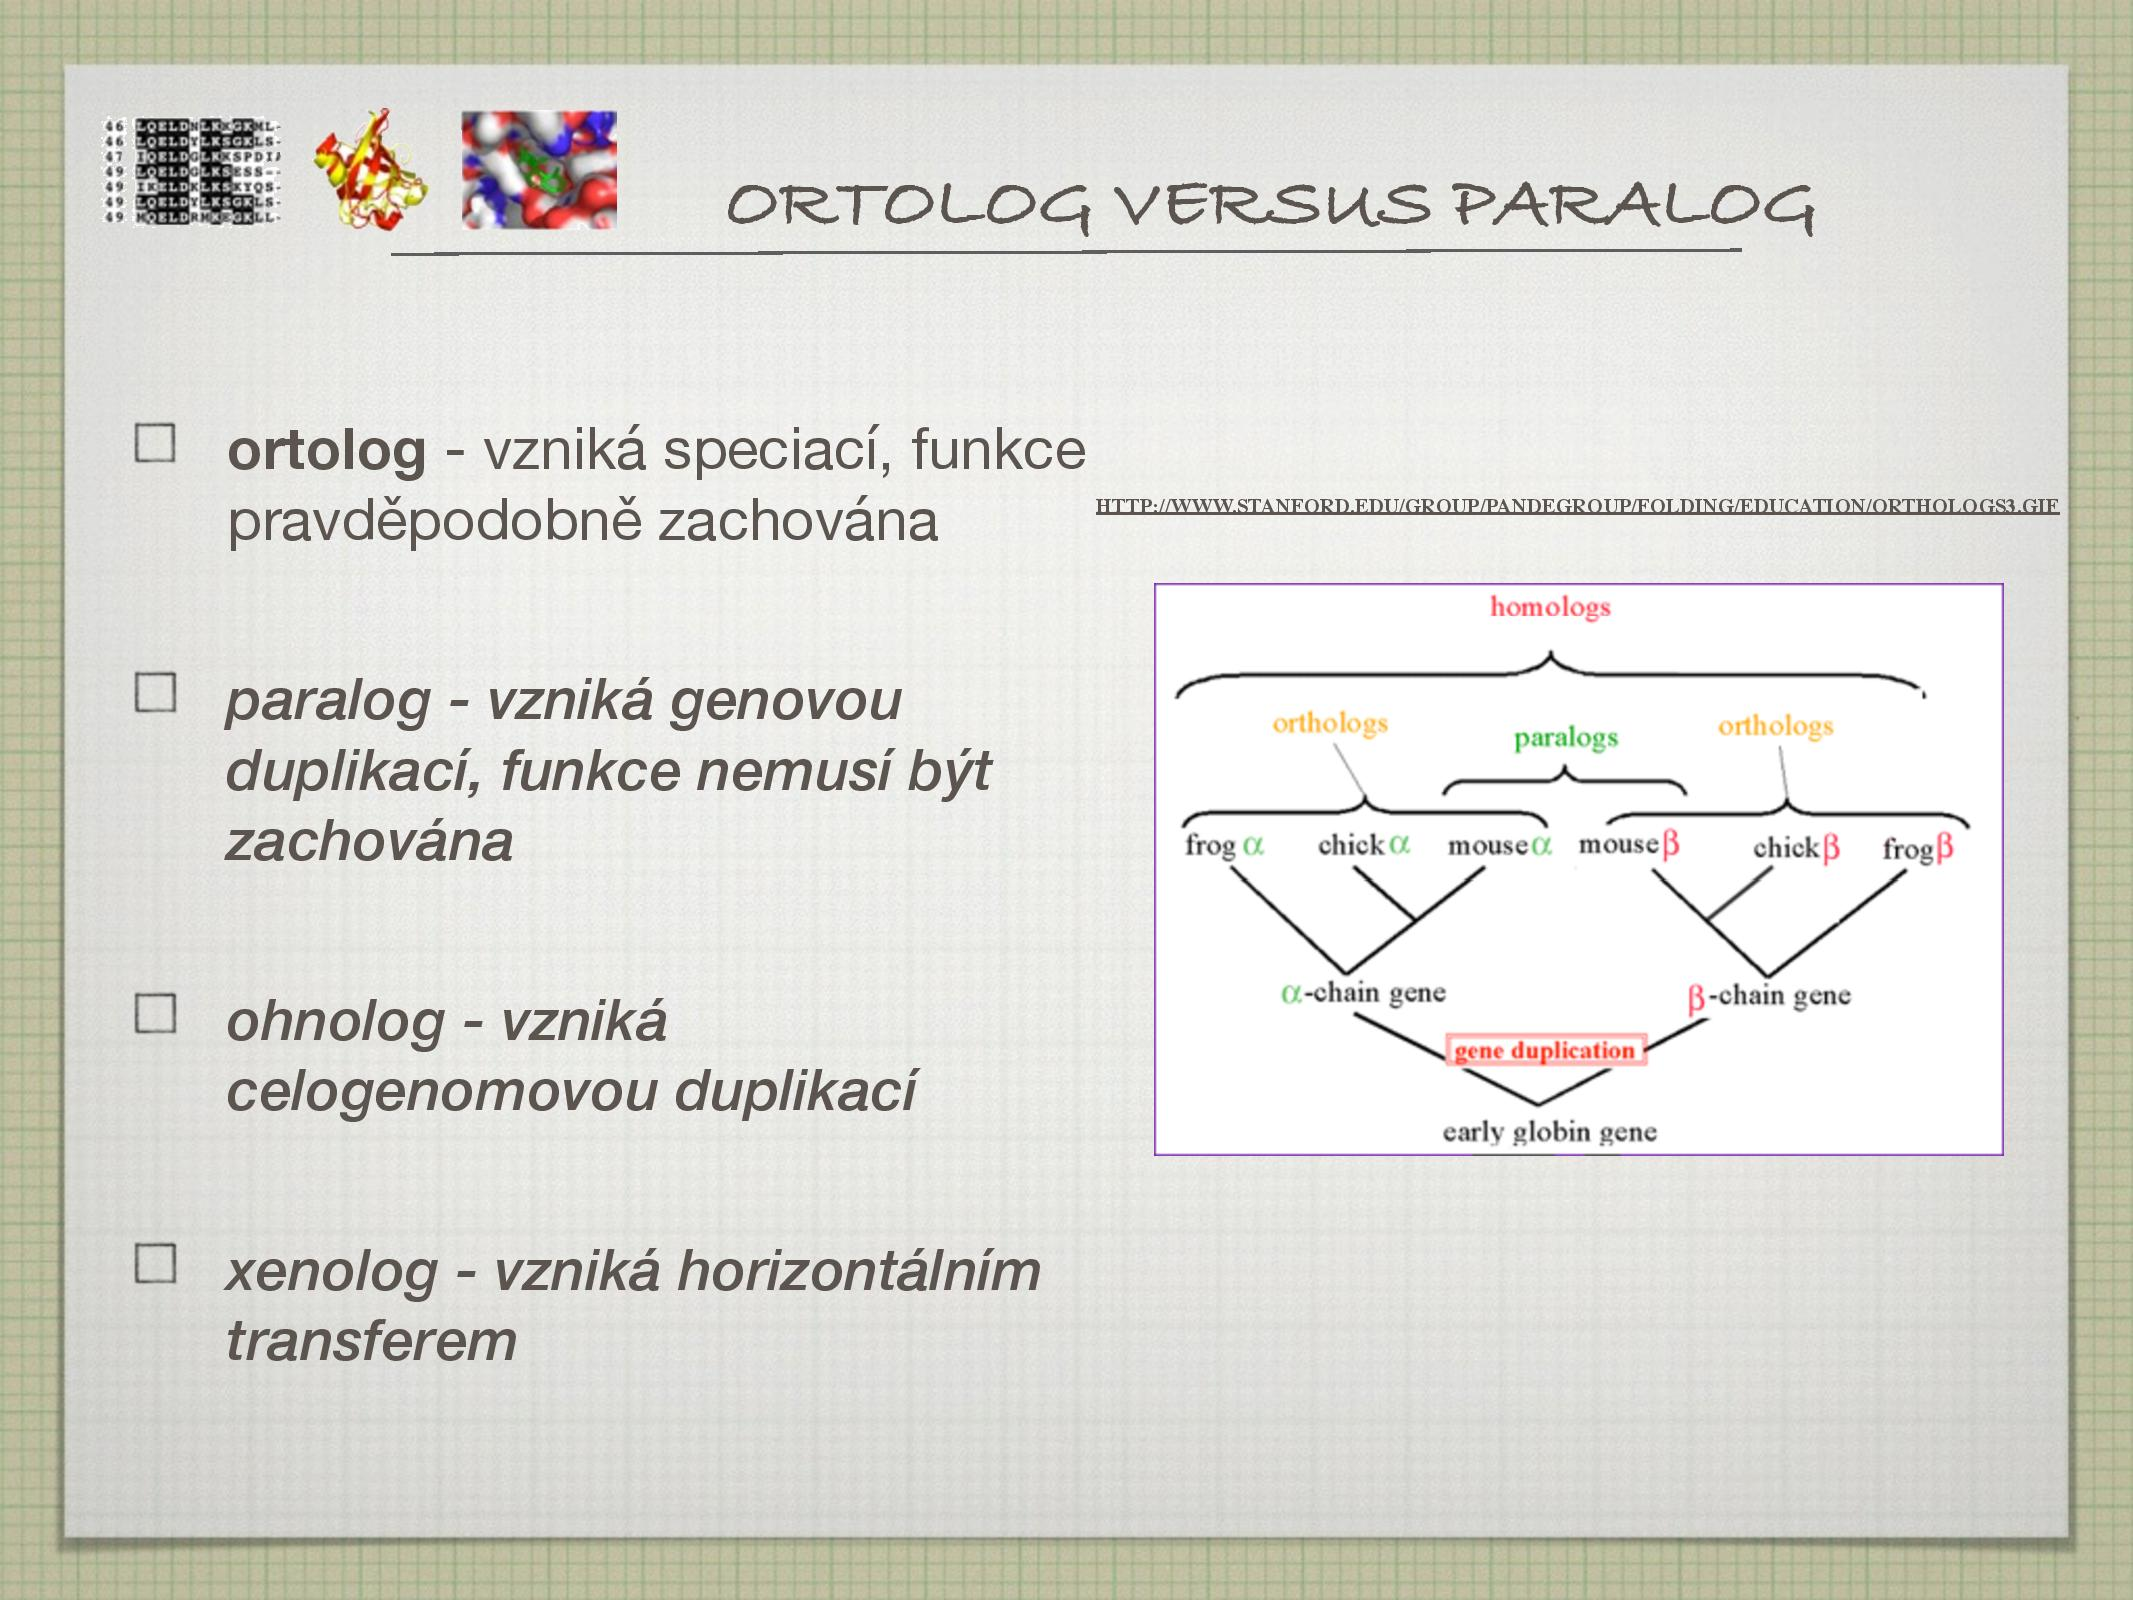
\includegraphics[width=0.85\textwidth]{slides-2/slide-27.jpg}
    \centering
    \label{slides-2-slide-27}
\end{figure}

\begin{description}
\item[A je homolog B]\hfill \\
A a B mají společného předka, jejich původní funkce však nemusí být zachována. Homologii můžeme (opatrně) odvodit z vyokého procenta sekvenční identita A a B (viz dále). Musíme však dát pozor na paralogii.

Na základě homologie můžeme (opatrně) odvodit funkční a strukturní podobnost. Například můžeme hledat homology problémových lidských proteinů v modelových organismech, na které budeme cílit vývíjená léčiva.


\item[A je ortolog B]\hfill \\
Poddruh homologie; A a B vznikly speciací ze společného předka, jejich funkce by tedy měla být zachována.


\item[A je paralog B]\hfill \\
Poddruh homologie; A a B vznikly genovou duplikací ze společného
předka --- jejich funkce tedy nemusí být zachována
(protože jedna kopie genu ji zastará, zatímco A a B se mohli vyvinout v něco jiného).


\item[A je ohnolog B]\hfill \\
Podobný vztah jako paralog, vzniká ale celogenomovou duplikací.


\item[A je xenolog B]\hfill \\
A a B vznikly horizontálním transferem (například mezidruhovým).


\item[A je analog B]\hfill \\
A a B mají podobnou funkci, avšak je to jen náhoda --- společného předka nemají.


\item[globální alignment]\hfill \\
Srovnávání celé sekvence.


\item[lokální alignment]\hfill \\
Srovnávání pouze částí sekvence, vybírá kousky, které k sobě sedí nejlépe.

\end{description}


\paragraph{Důvod srovnávání sekvencí}
\begin{itemize}[nosep]
    \item nalezení evoluční podobnosti (analogie, homologie)
    \item získání informací o struktuře, funkci, a evolučním vývoji proteinu
\begin{itemize}[nosep]
    \item pomocí srovnání s proteiny, které už mají známou strukturu, funkci a původ
\end{itemize}

    \item nalezení aktivních (konzervovaných) míst
    \item nalezení mutantů
    \item možno pomocí něj dát smysl velkému množství biologických dat
\end{itemize}



Snažíme se ze znalosti struktury a funkce určitého proteinu odvodit funkci jiného, podobného (homologního) proteinu. To, jestli je vůbec možné z kvantitativní veličiny sekvenční identity (SI) vyvodit kvalitativní rozhodnutí o homologii, zkoumali \textbf{Chotia, Lest} (1986) a \textbf{Rost} (1999). Zjistilo se, že \textbf{změny ve struktuře jsou korelovány se změnami v sekvenci}, neboli z \%SI si můžeme troufnout odvodit homologii a podobné vztahy, a z nich poté hádat věci jako je funkce nebo evoluční původ.

\begin{figure}
    \caption{Prezentace č. 2, slide č. 31}
    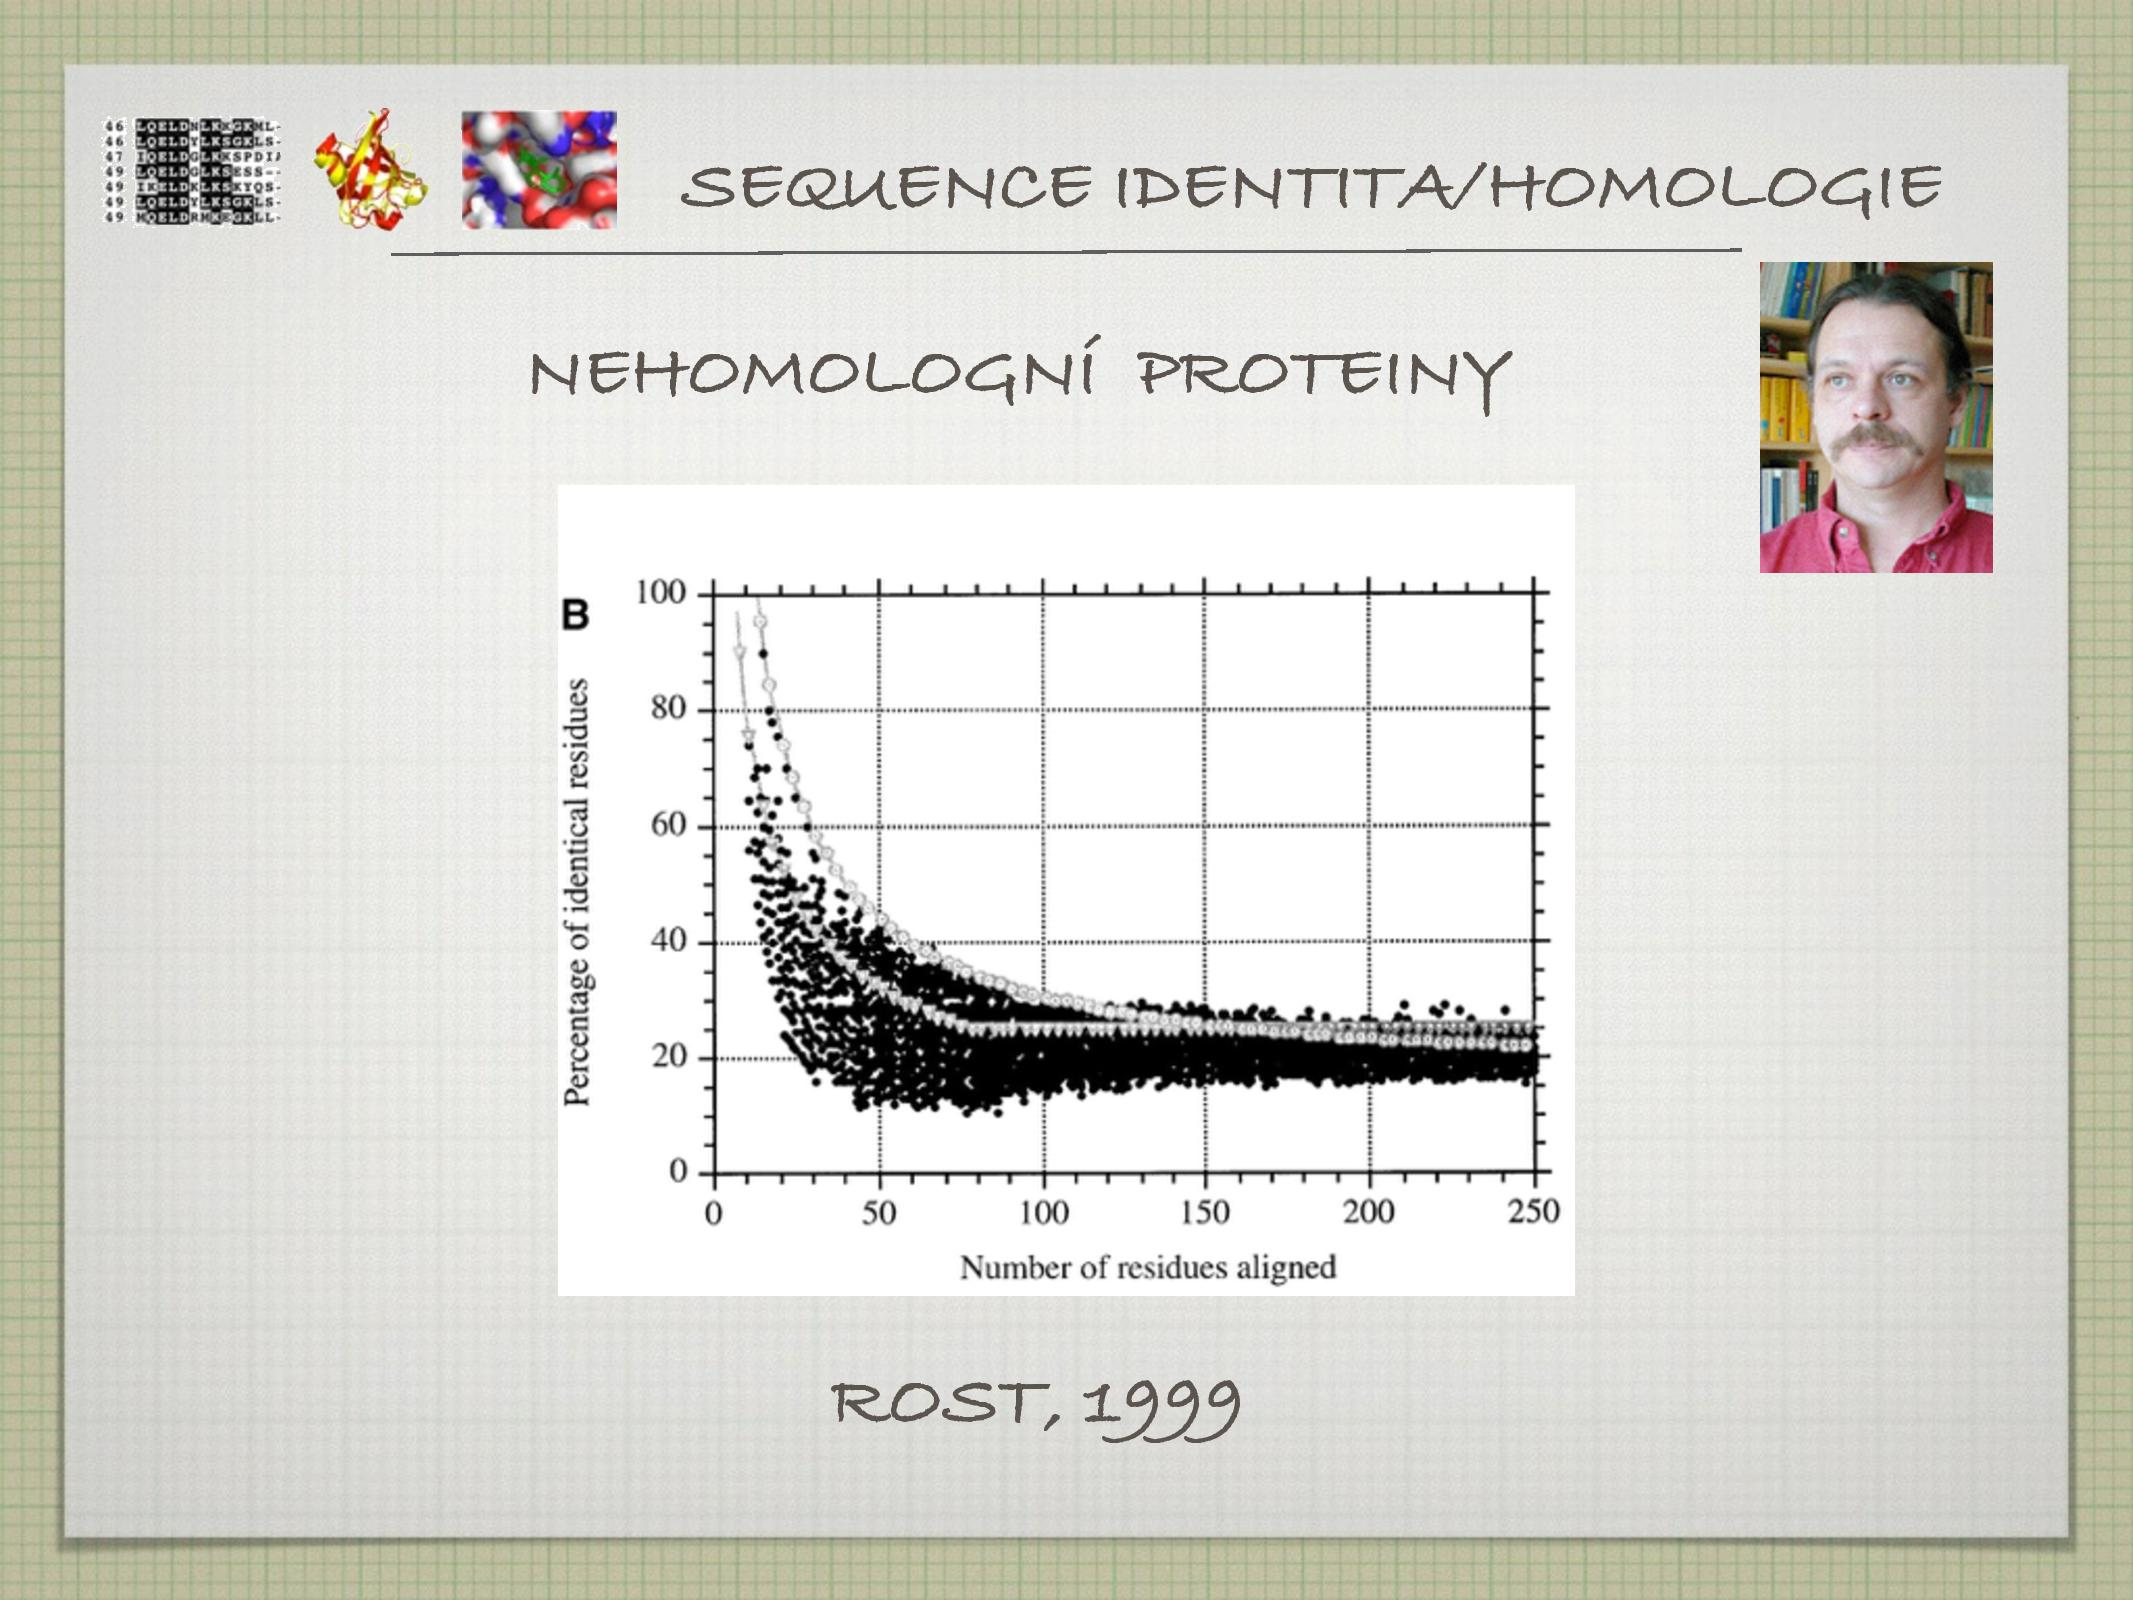
\includegraphics[width=0.85\textwidth]{slides-2/slide-31.jpg}
    \centering
    \label{slides-2-slide-31}
\end{figure}
\begin{figure}
    \caption{Prezentace č. 2, slide č. 32}
    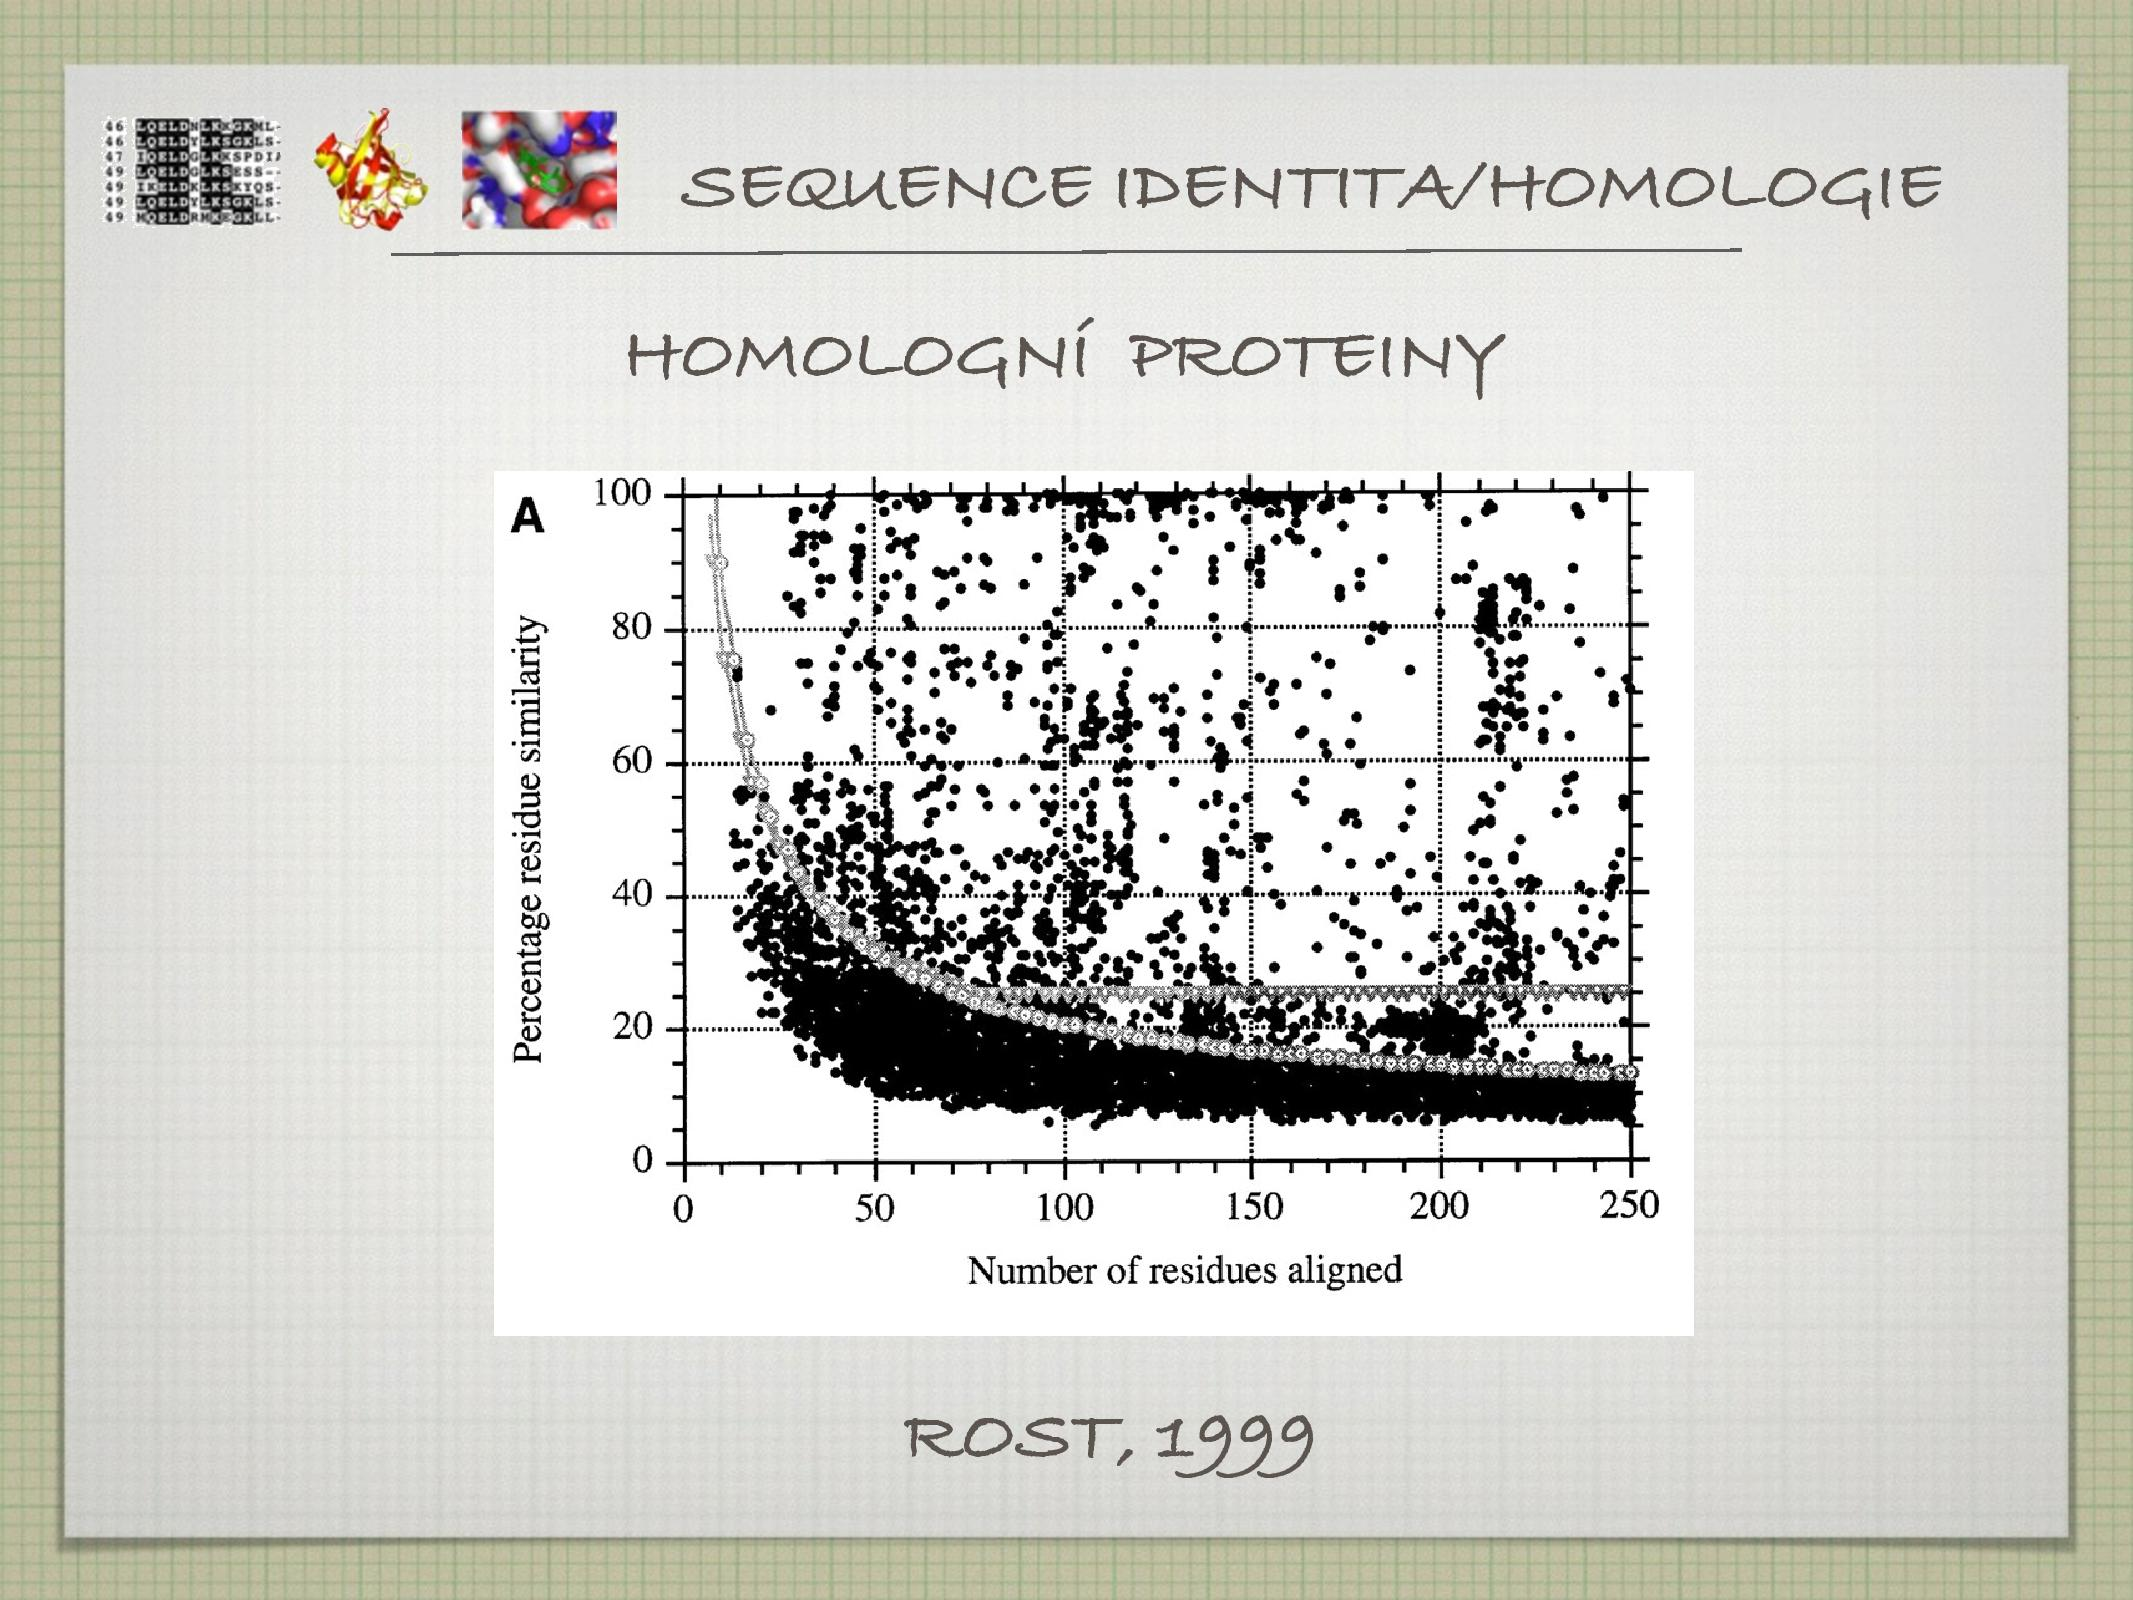
\includegraphics[width=0.85\textwidth]{slides-2/slide-32.jpg}
    \centering
    \label{slides-2-slide-32}
\end{figure}
\begin{figure}
    \caption{Prezentace č. 2, slide č. 39}
    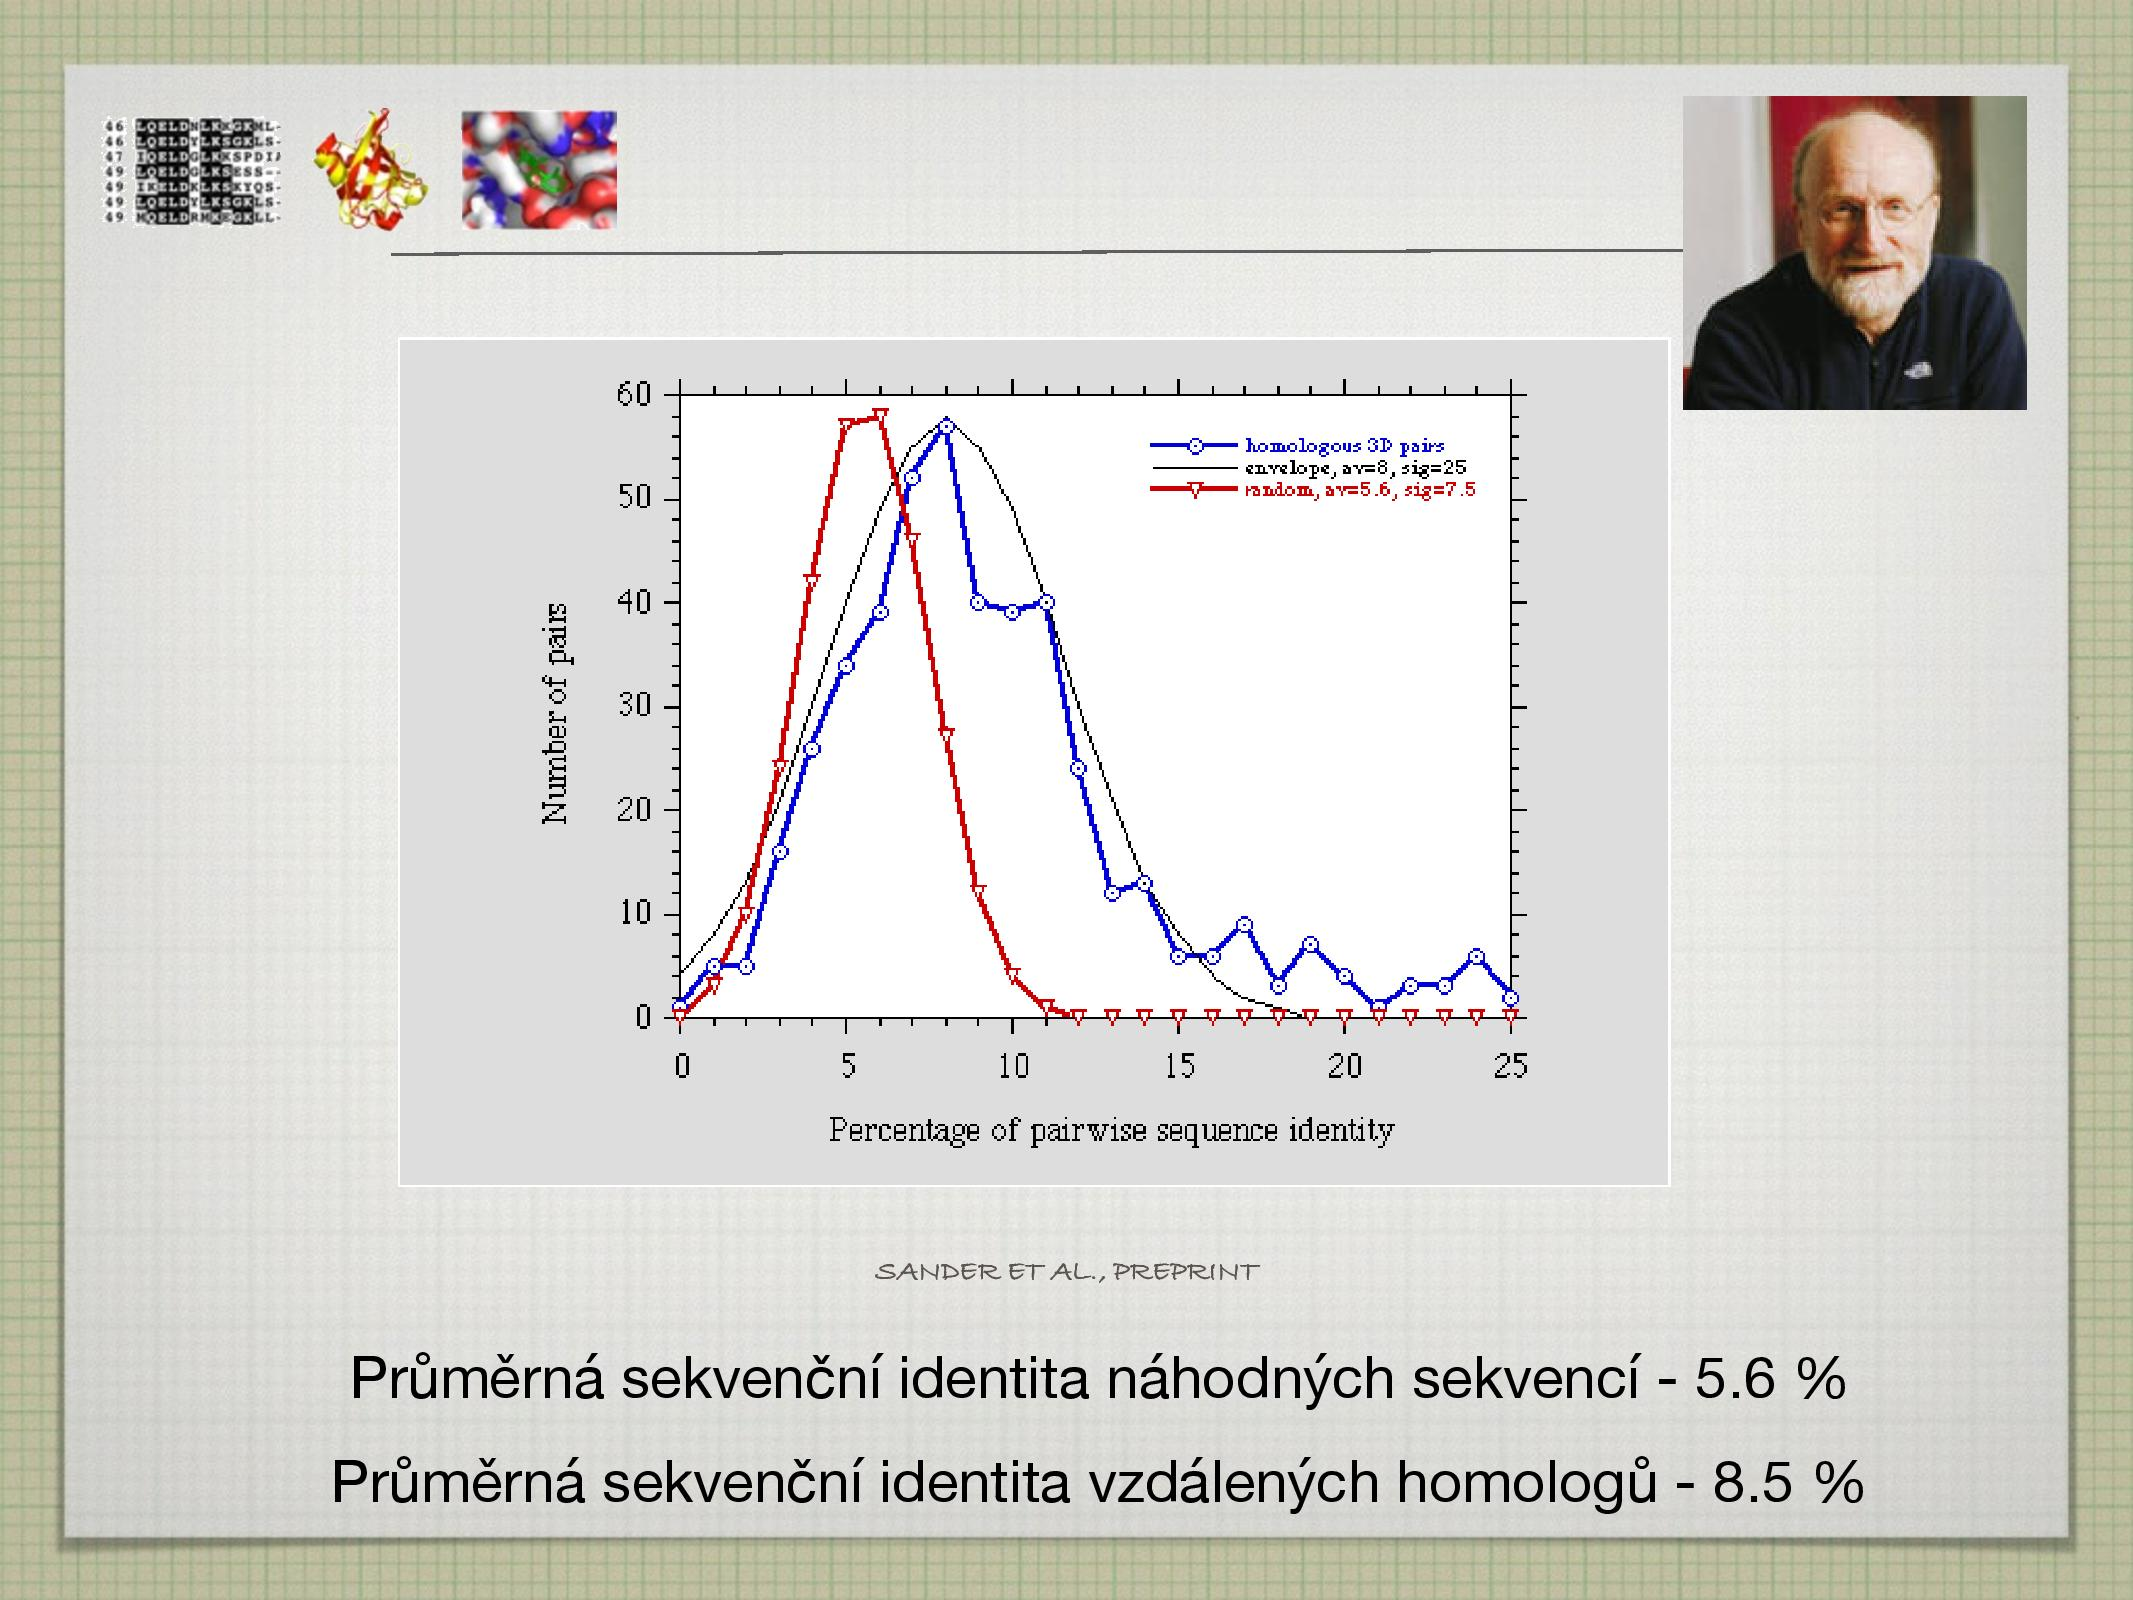
\includegraphics[width=0.85\textwidth]{slides-2/slide-39.jpg}
    \centering
    \label{slides-2-slide-39}
\end{figure}

\paragraph{Sekvenční identita (SI)}
\begin{itemize}[nosep]
    \item hranice relevatní pro potenciální homologii (určené Rostem)
\begin{itemize}[nosep]
    \item \(\text{SI} > 35\%\) naznačuje možnou homologii
    \item \(20\% < \text{SI} < 35\%\) je takzvaná \emph{twilight zone}, homologie je možná
    \item \(\text{SI} < 20\%\), o homologi nemůžeme s jistotou říct vůbec nic
\end{itemize}

    \item průměrná SI náhodných sekvencí je asi 5,9\%
    \item průměrná SI vzdálených homologů je asi 8,5\%
    \item existuje více metod, jak SI vypočítat (a SI se u každé metody liší)
\begin{itemize}[nosep]
    \item počet náhodných pozic / délka alignmentu
    \item počet shodných pozic / délka kratší sekvence
    \item počet shodných pozic / průměrná délka sekvencí
\end{itemize}

\end{itemize}



Jakým způsbem se rozhodnout, když jsme v twilight zóně? Na to existuje několik triků.

\paragraph{Jak z twilight zóny?}
\begin{itemize}[nosep]
    \item pokud jsou vyměněny kladně nabité AK za jiné kladně nabité AK, alanin za valin atp. (zkrátka tzv. \emph{konzervativní záměny}), sekvence jsou nejspíše homologní
    \item pokud se snažíme zjistit něco více o homologii A a B, stačí najít C, které je homologické s A a zároveň je i homologické s B; z toho totiž plyne, že A i B jsou také homologické
\end{itemize}



Výše bylo zmíněno, že srovnávání sekvencí funguje jak pro proteiny, tak pro DNA. Přesto se ale častěji, minimálně k určování homologie, používají proteiny, a to ze dvou důvodů:
\begin{enumerate}[nosep]
    \item protože AK je dvacet, je menší šance, že budou na jednom místě dvě shodné AK náhodou (oproti čtyřem nukleotidům v DNA, kde je náhodná shoda pravděpodobnější)
    \item různé kodony kódují stejné AK, čili určité změny v DNA kódu se vůbec nemusí projevit v jeho exprimaci; jinými slovy, i relativně hodně odlišné sekvence mohou kódovat stejné, nebo velice podobné proteiny
\end{enumerate}



Srovnávání sekvencí DNA ale má svá uplatnění. Používá se v místech, která se v proteomu vůbec neobjeví; při zkoumání regulačních oblastní genů a definování genů a při celogenomovém srovnávání.

Metody jsou v zásadě dvě, \textbf{dotploty}, které slouží spíše k hrubému odhadu situace, a \textbf{pairwise sequence alignment}, což je aby se řeklo \emph{the real deal}.

\section{Dotplot} \label{Dotplot}


\begin{figure}
    \caption{Prezentace č. 2, slide č. 45}
    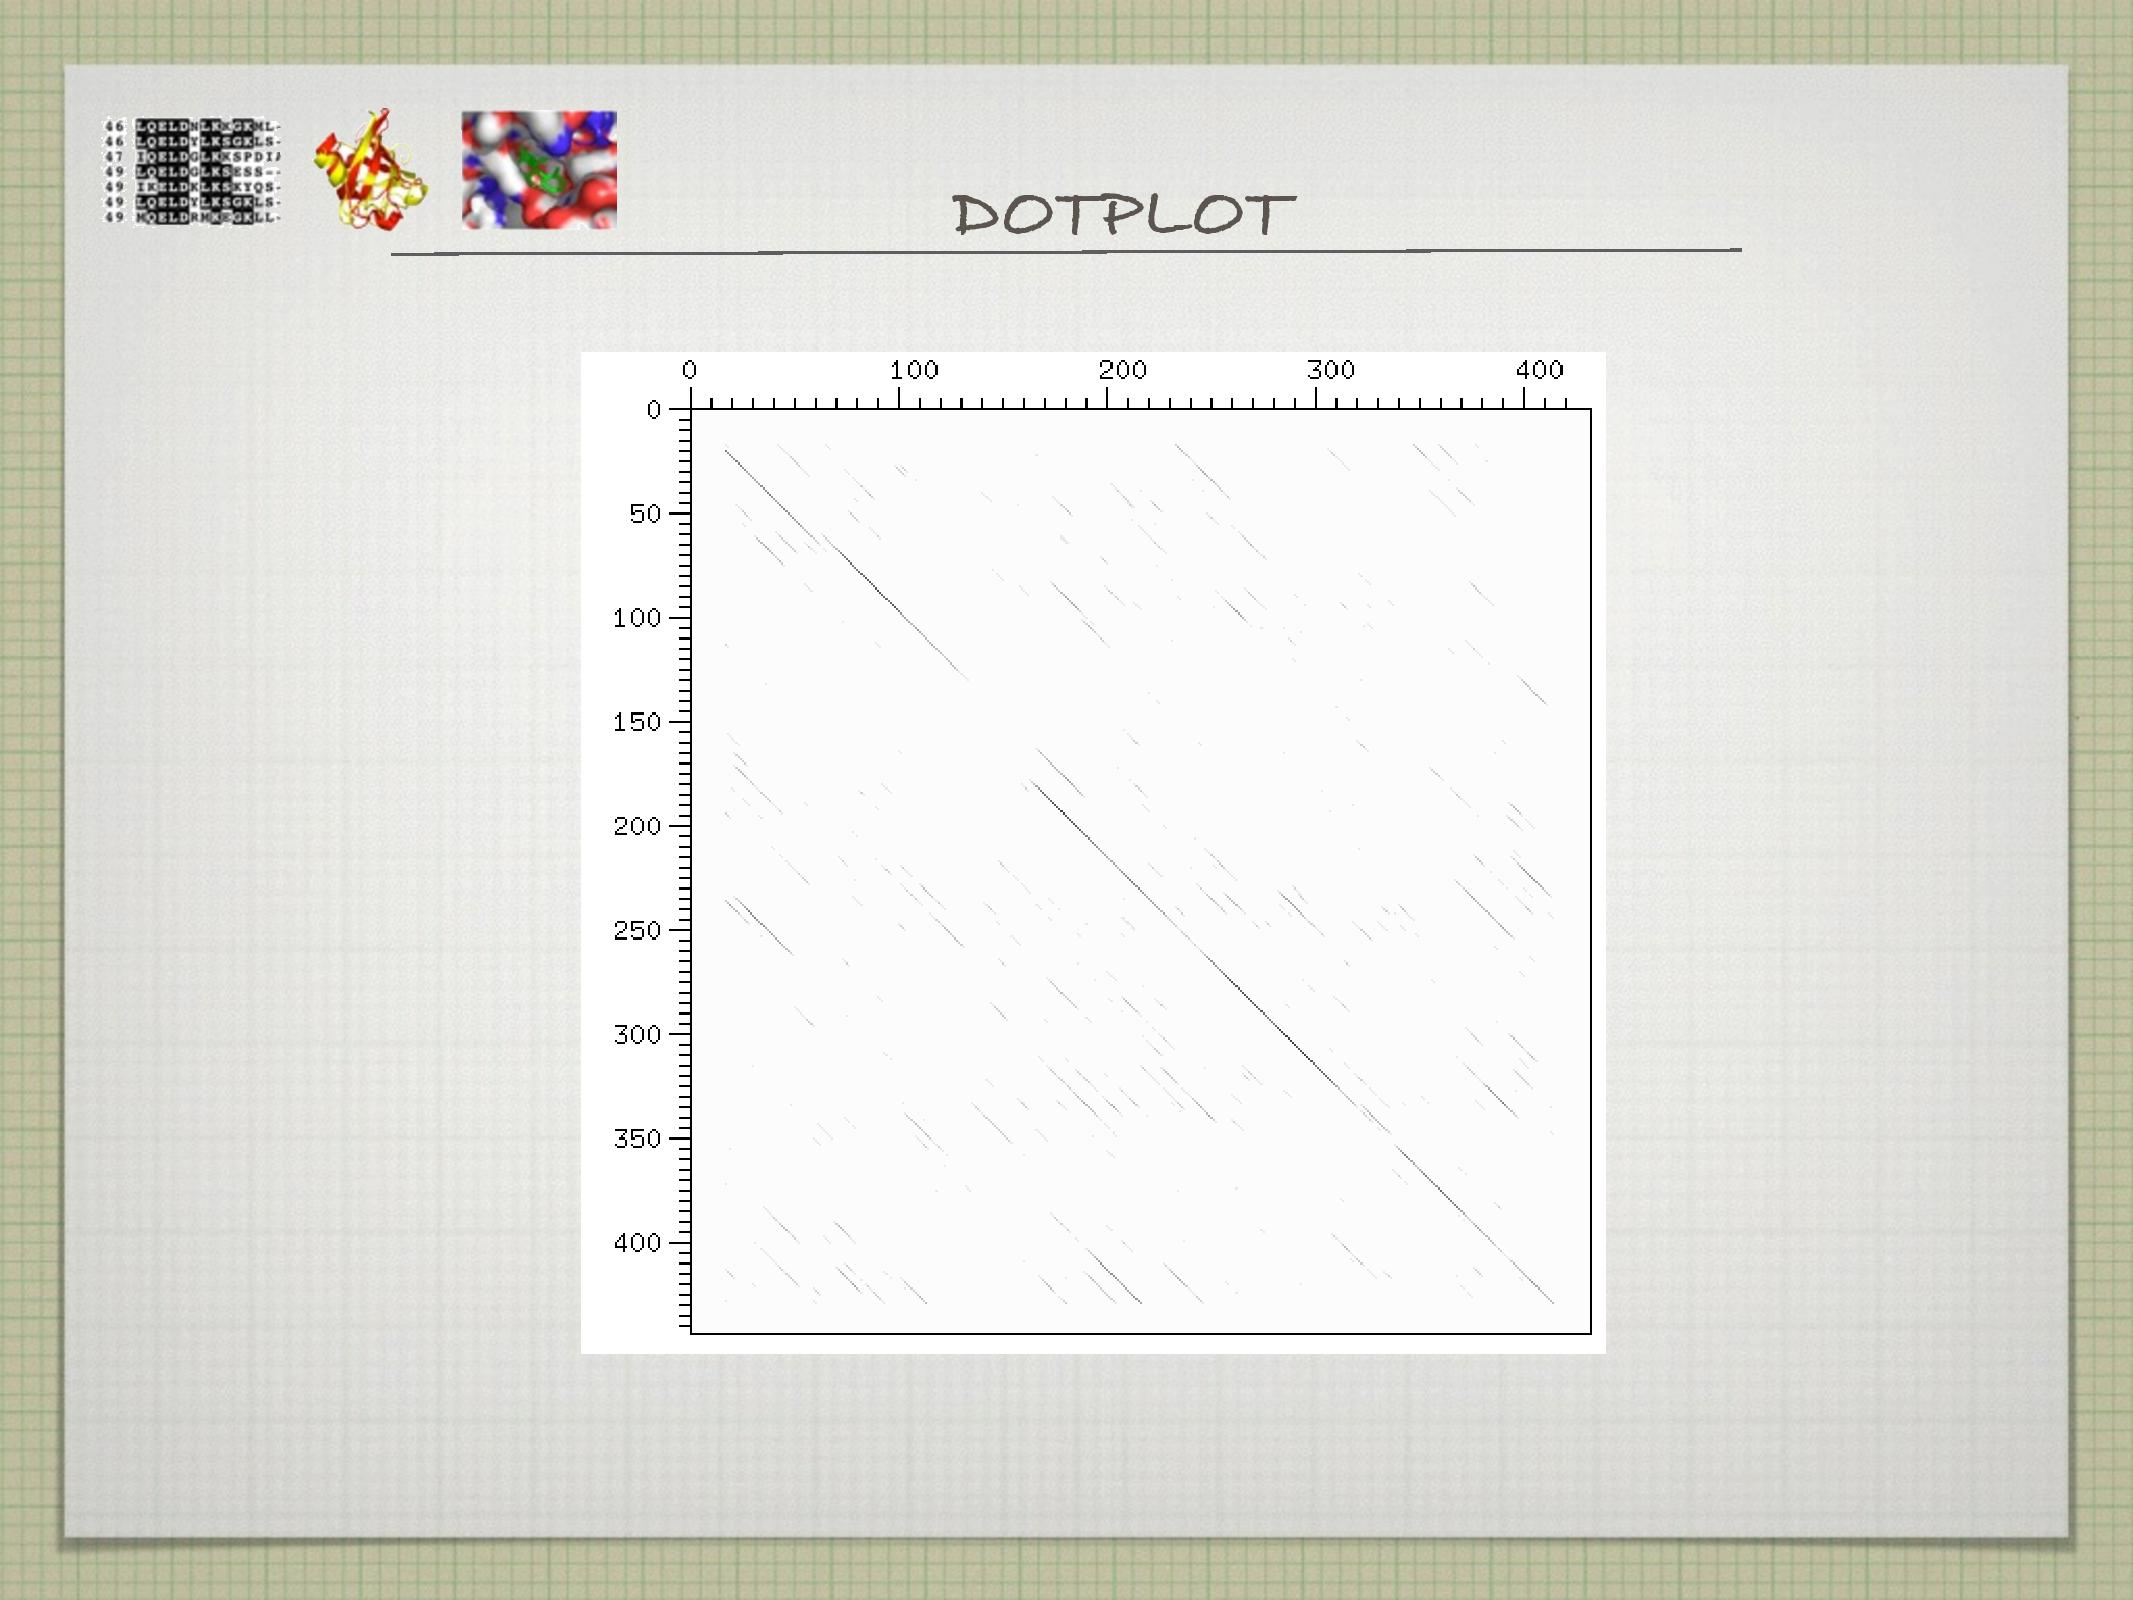
\includegraphics[width=0.85\textwidth]{slides-2/slide-45.jpg}
    \centering
    \label{slides-2-slide-45}
\end{figure}
\begin{figure}
    \caption{Prezentace č. 2, slide č. 50}
    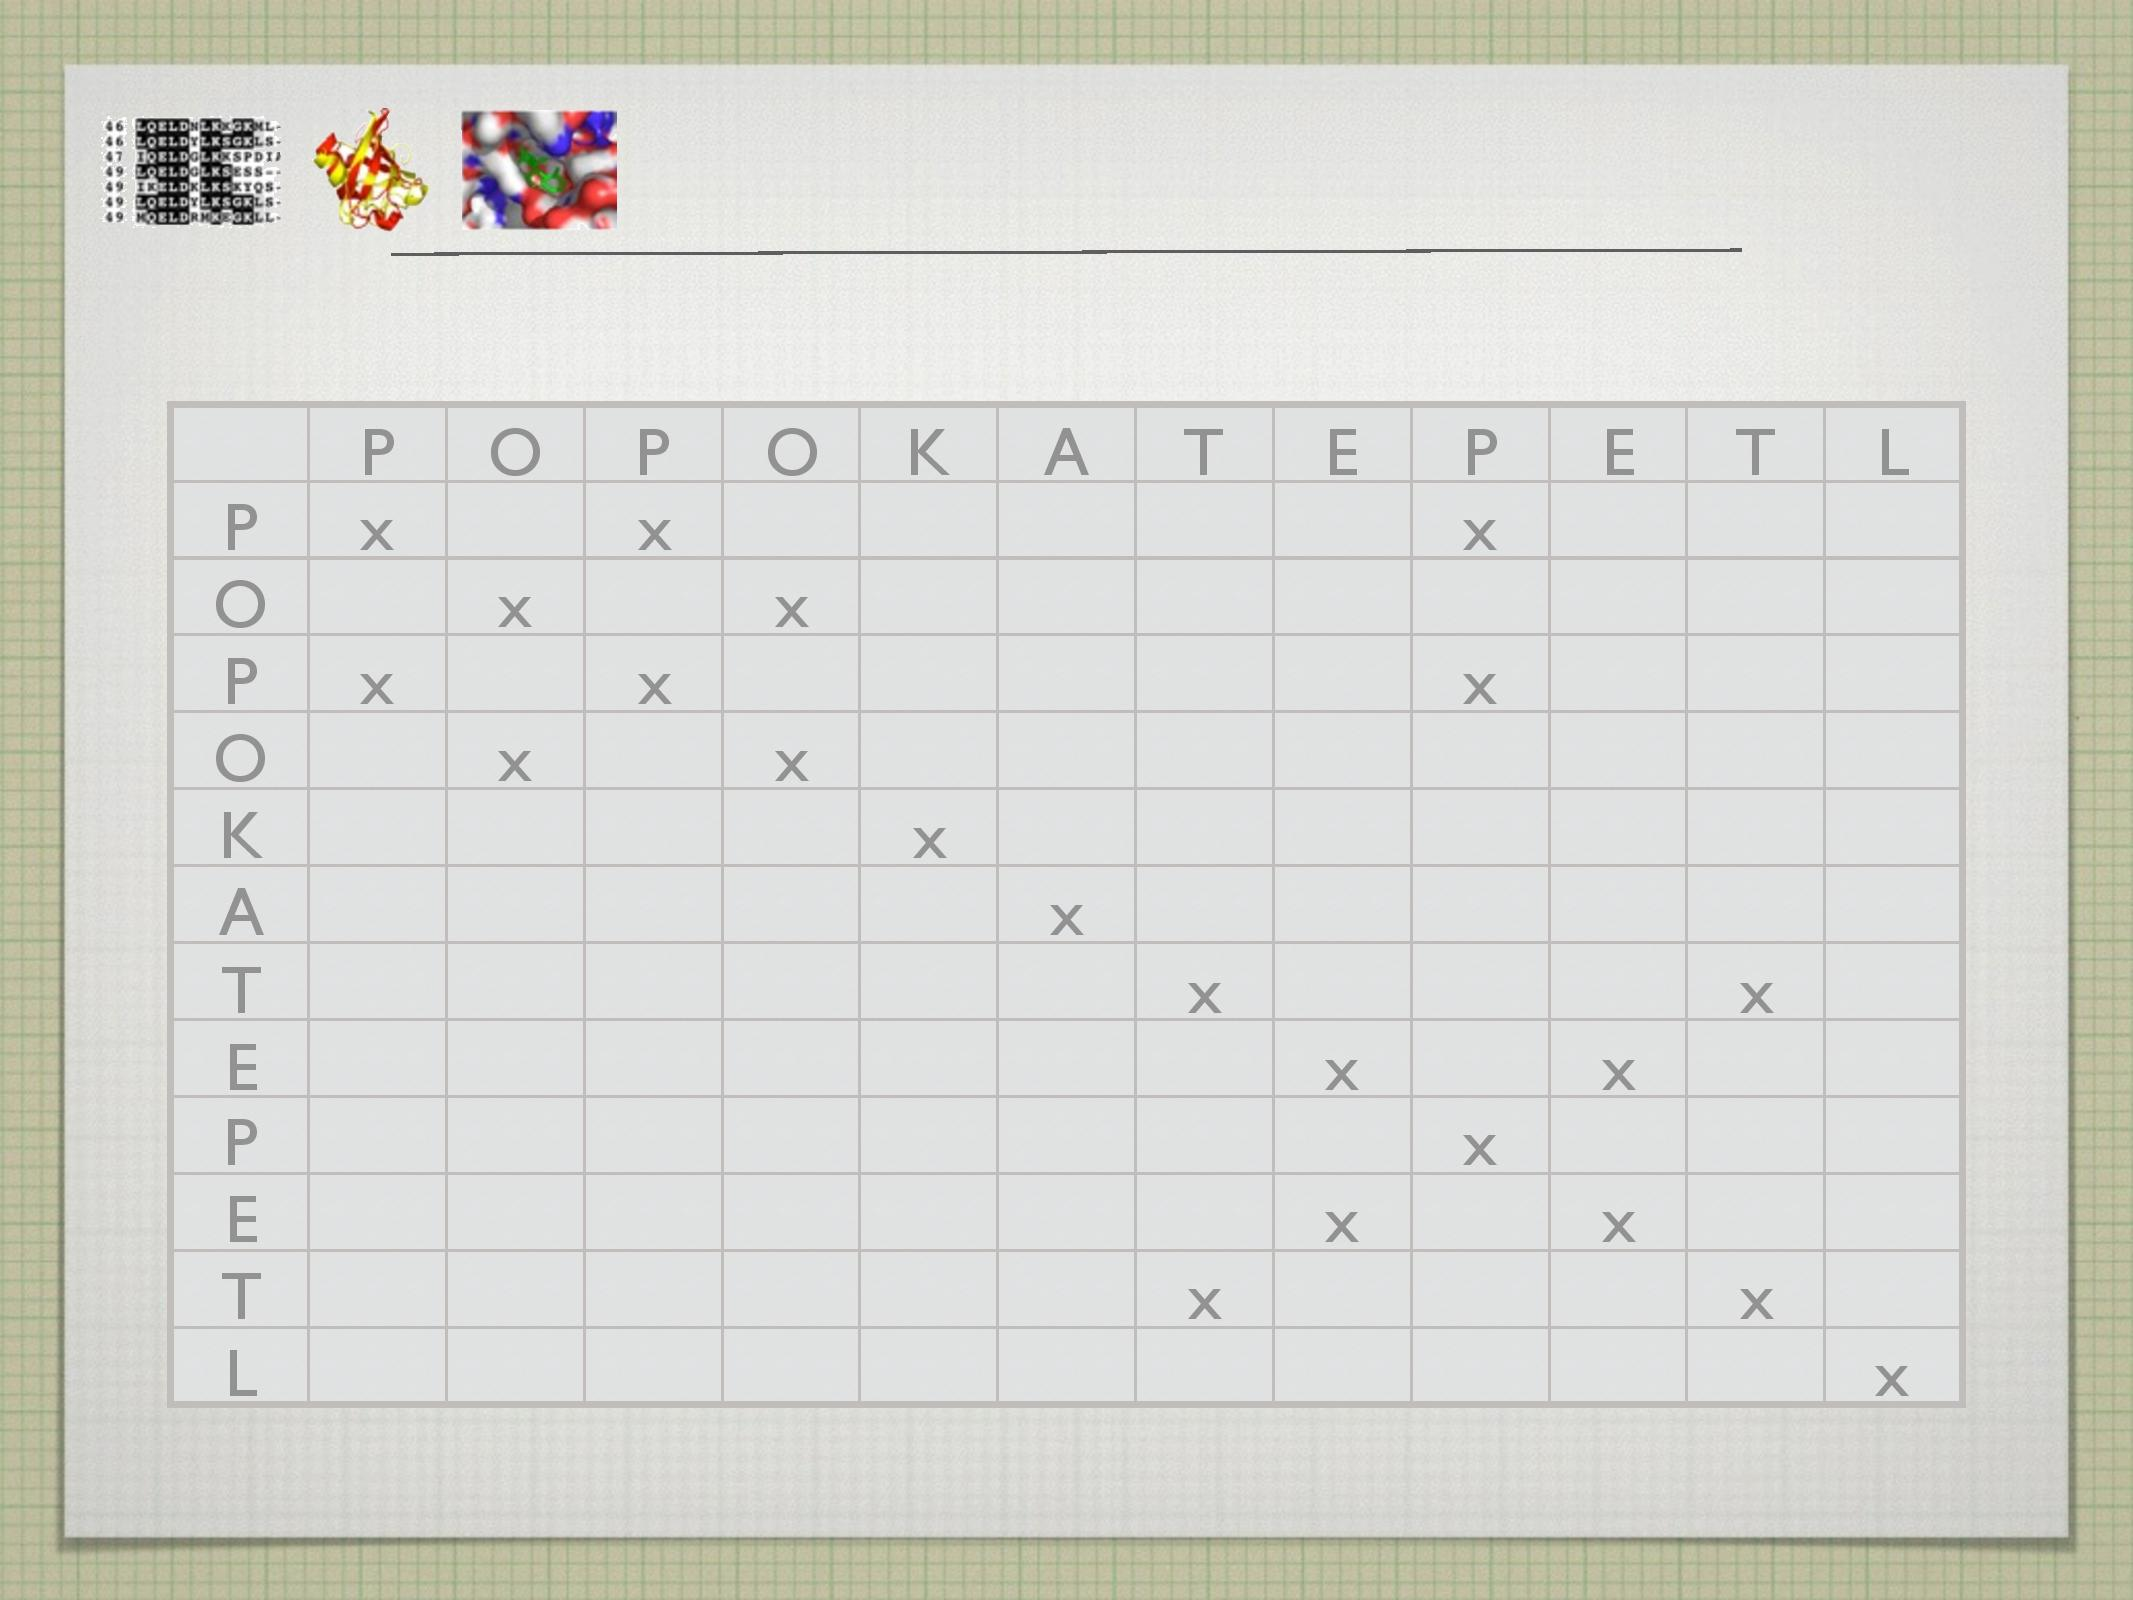
\includegraphics[width=0.85\textwidth]{slides-2/slide-50.jpg}
    \centering
    \label{slides-2-slide-50}
\end{figure}
\begin{figure}
    \caption{Prezentace č. 2, slide č. 55}
    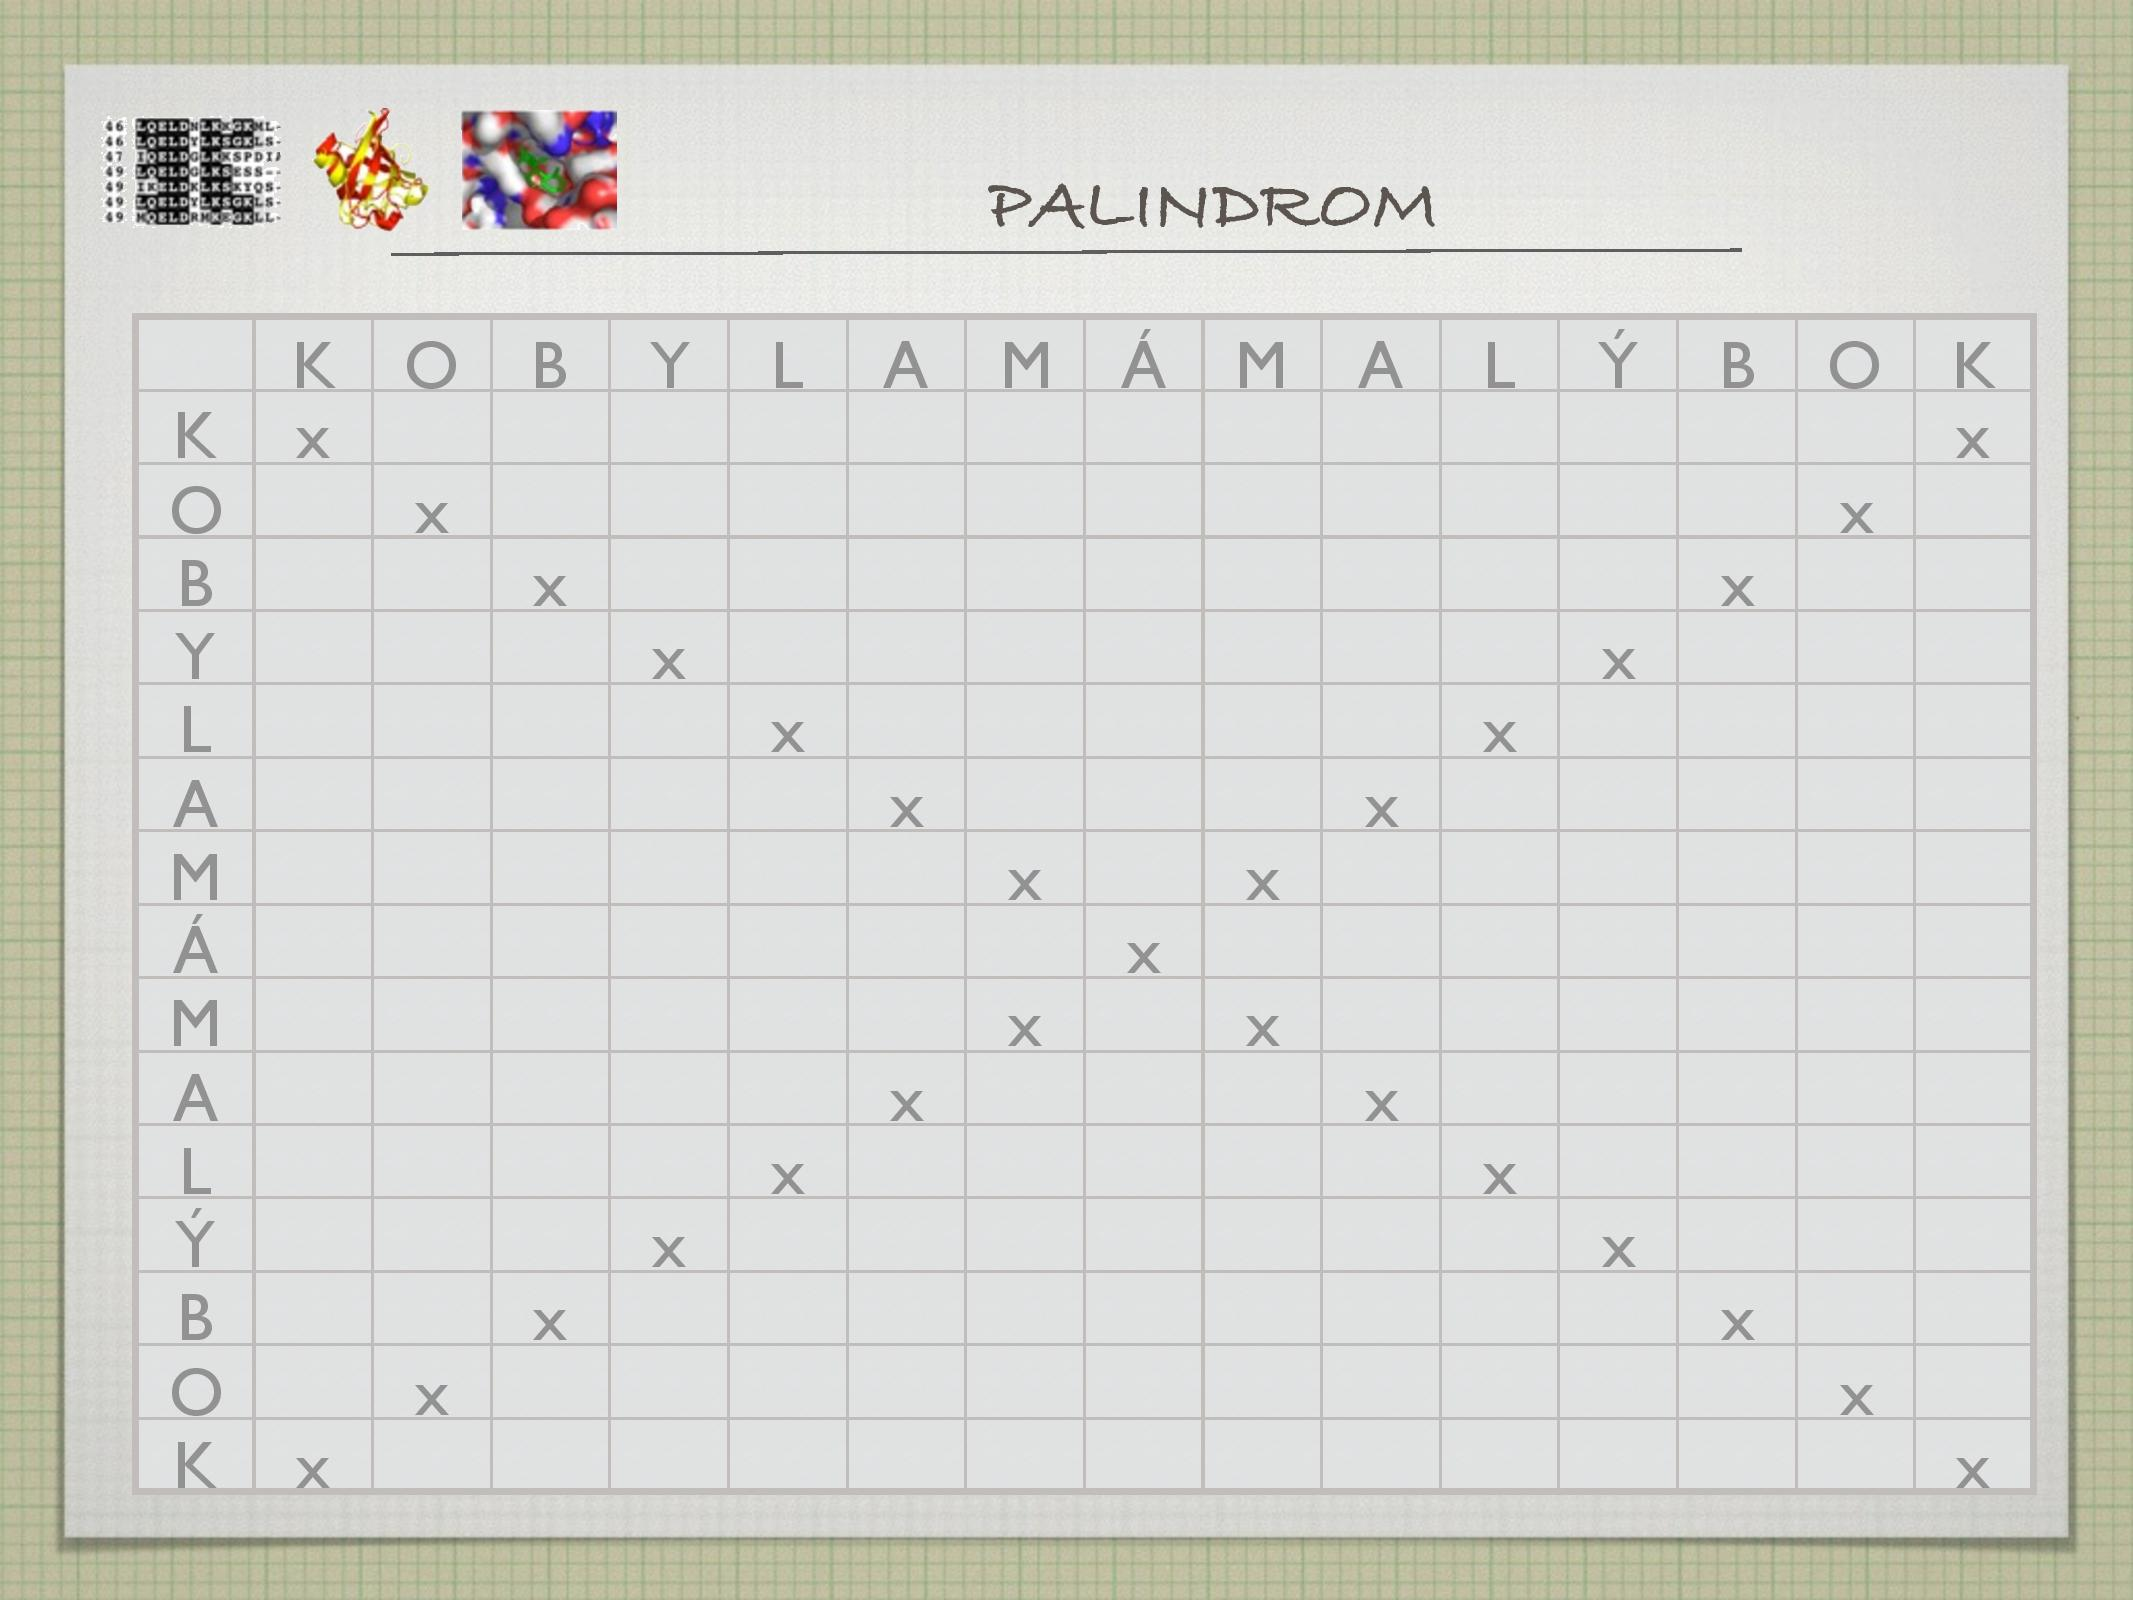
\includegraphics[width=0.85\textwidth]{slides-2/slide-55.jpg}
    \centering
    \label{slides-2-slide-55}
\end{figure}
\begin{figure}
    \caption{Prezentace č. 2, slide č. 57}
    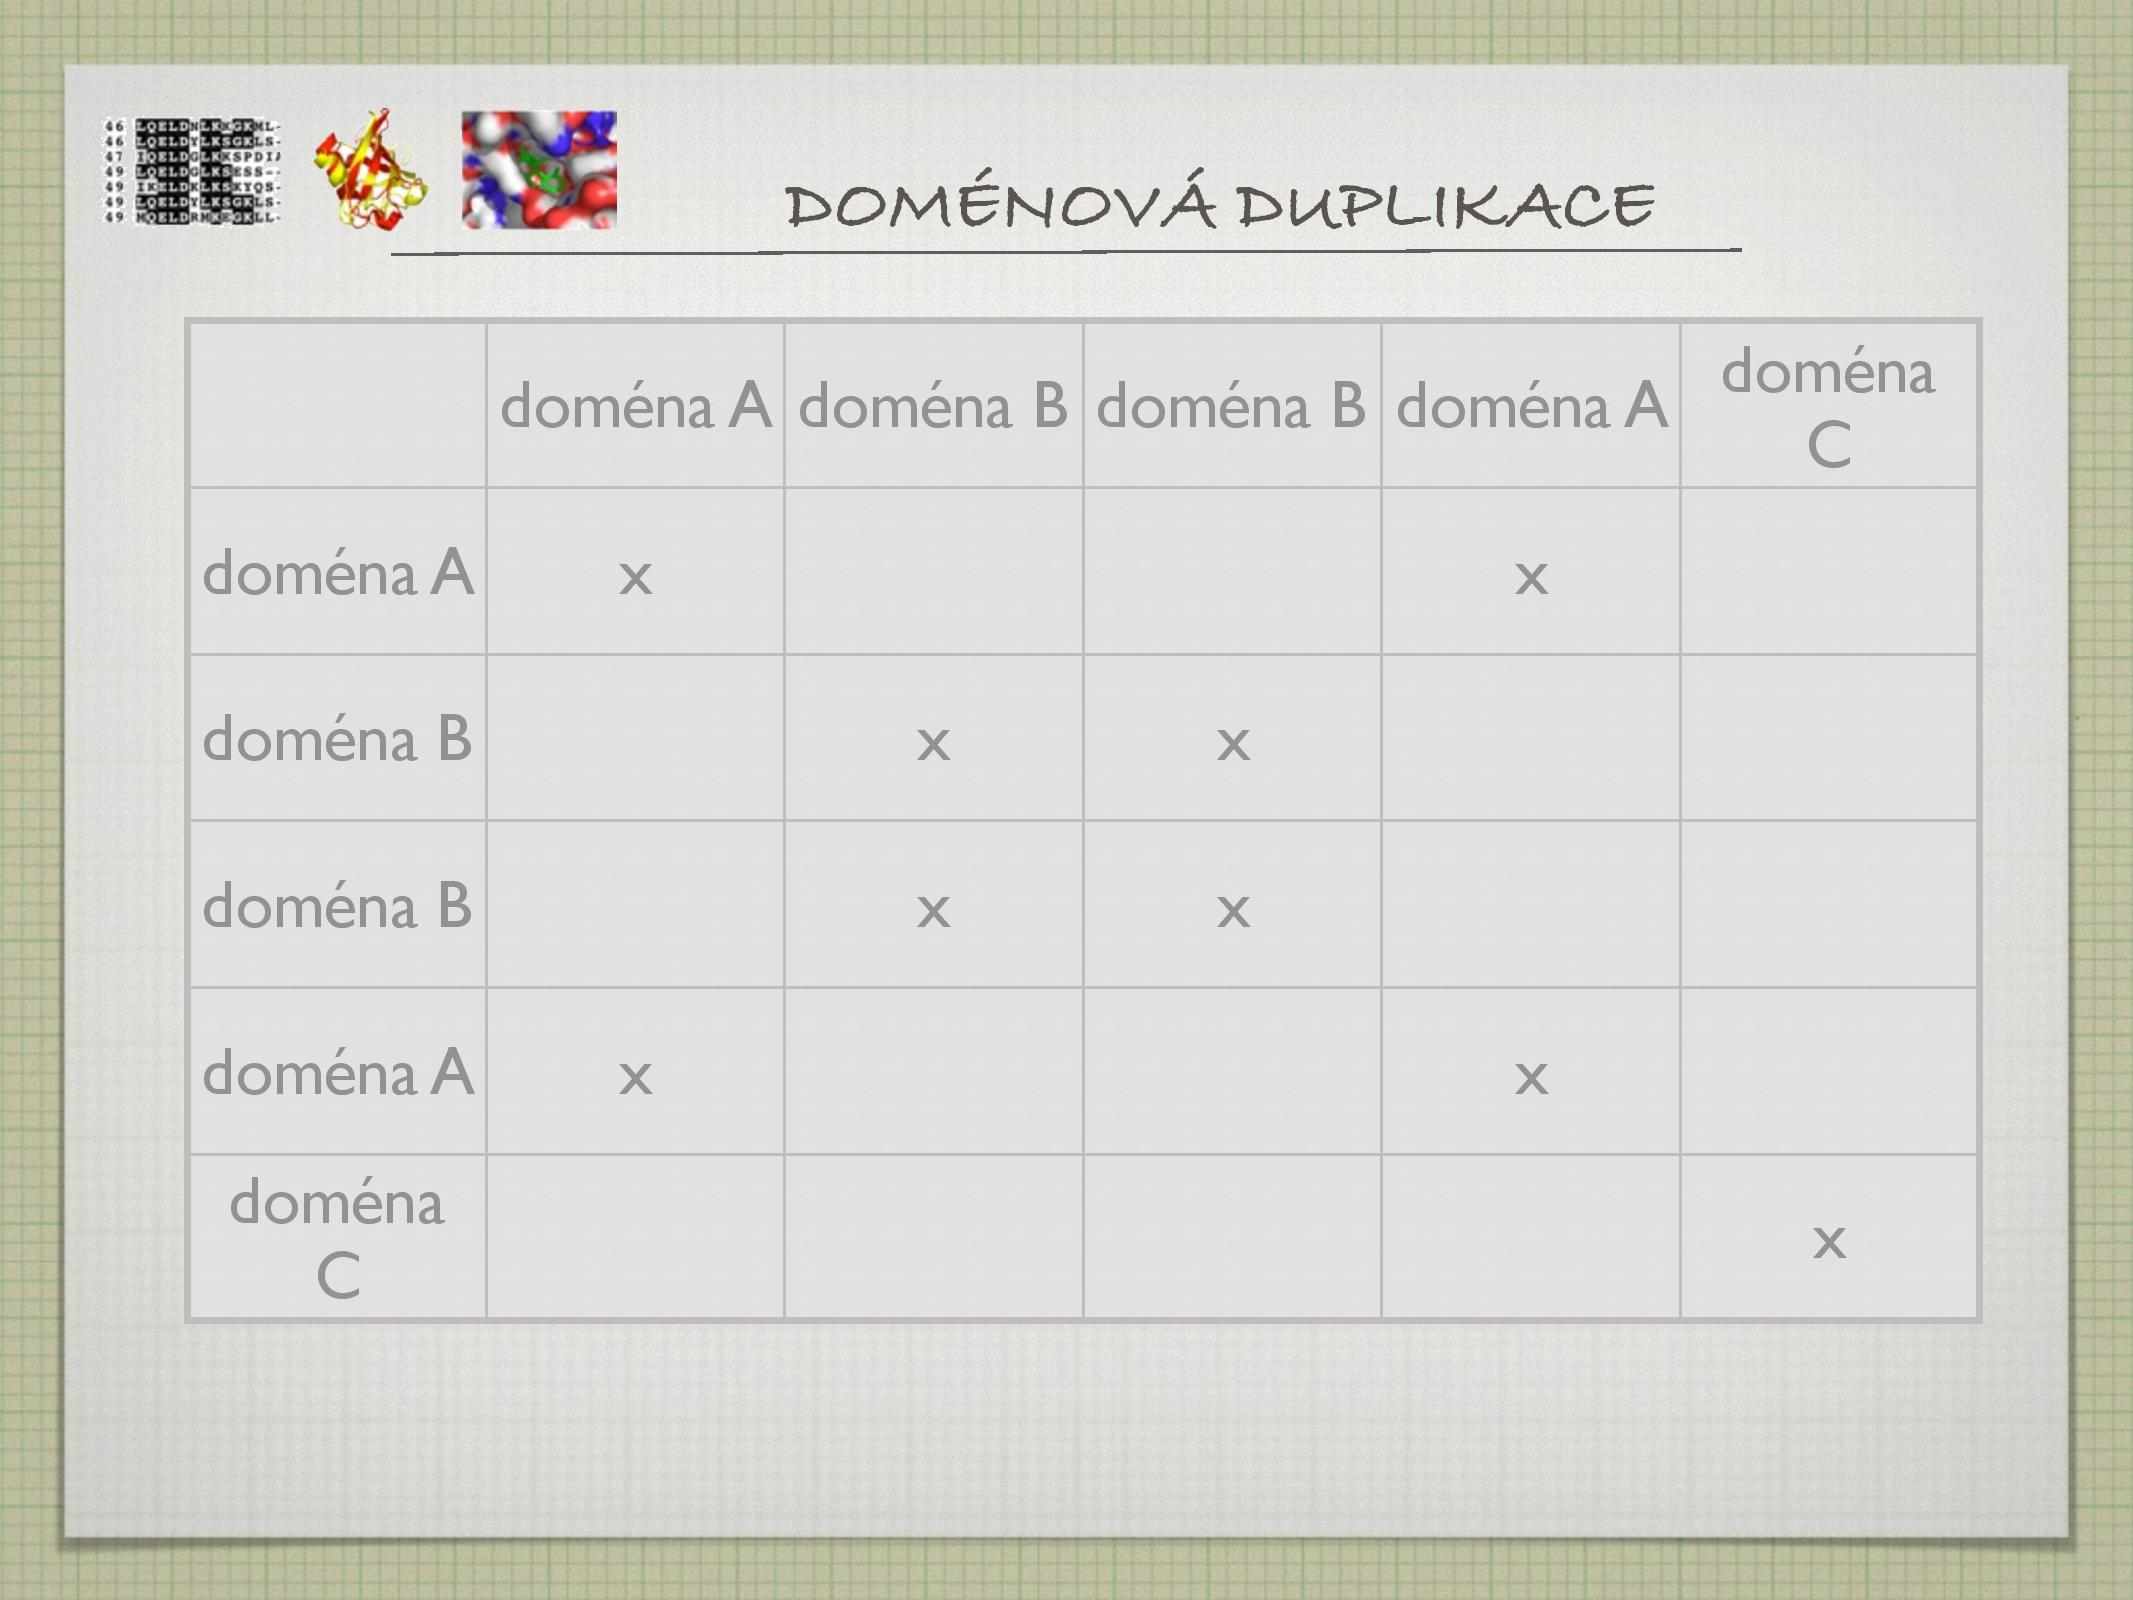
\includegraphics[width=0.85\textwidth]{slides-2/slide-57.jpg}
    \centering
    \label{slides-2-slide-57}
\end{figure}

Nejpřímější a nejjednodušší metoda: do tabulky se zaznamenávají místa, na kterých jsou dvě sekvence shodné (viz slidy). Někdy se místo jednotlivých stavebních jednotek sekvencí používají celé domény na sekvencích.

Na dotplotu byly sledovány i první dvě známé struktury, hemoglobin a myoglobin.

\paragraph{Silné stránky}
\begin{itemize}[nosep]
    \item jednoduchý a rychlý
    \item odhaluje repetice, inverze, přeházené domény, oblastni s nízkou komplexitou
    \item poskytuje návod, kde má vůbec smysl dělat podrobnější sequence alignment
    \item vhodný pro odhad podobnosti sekvencí
\end{itemize}



\begin{figure}
    \caption{Prezentace č. 2, slide č. 60}
    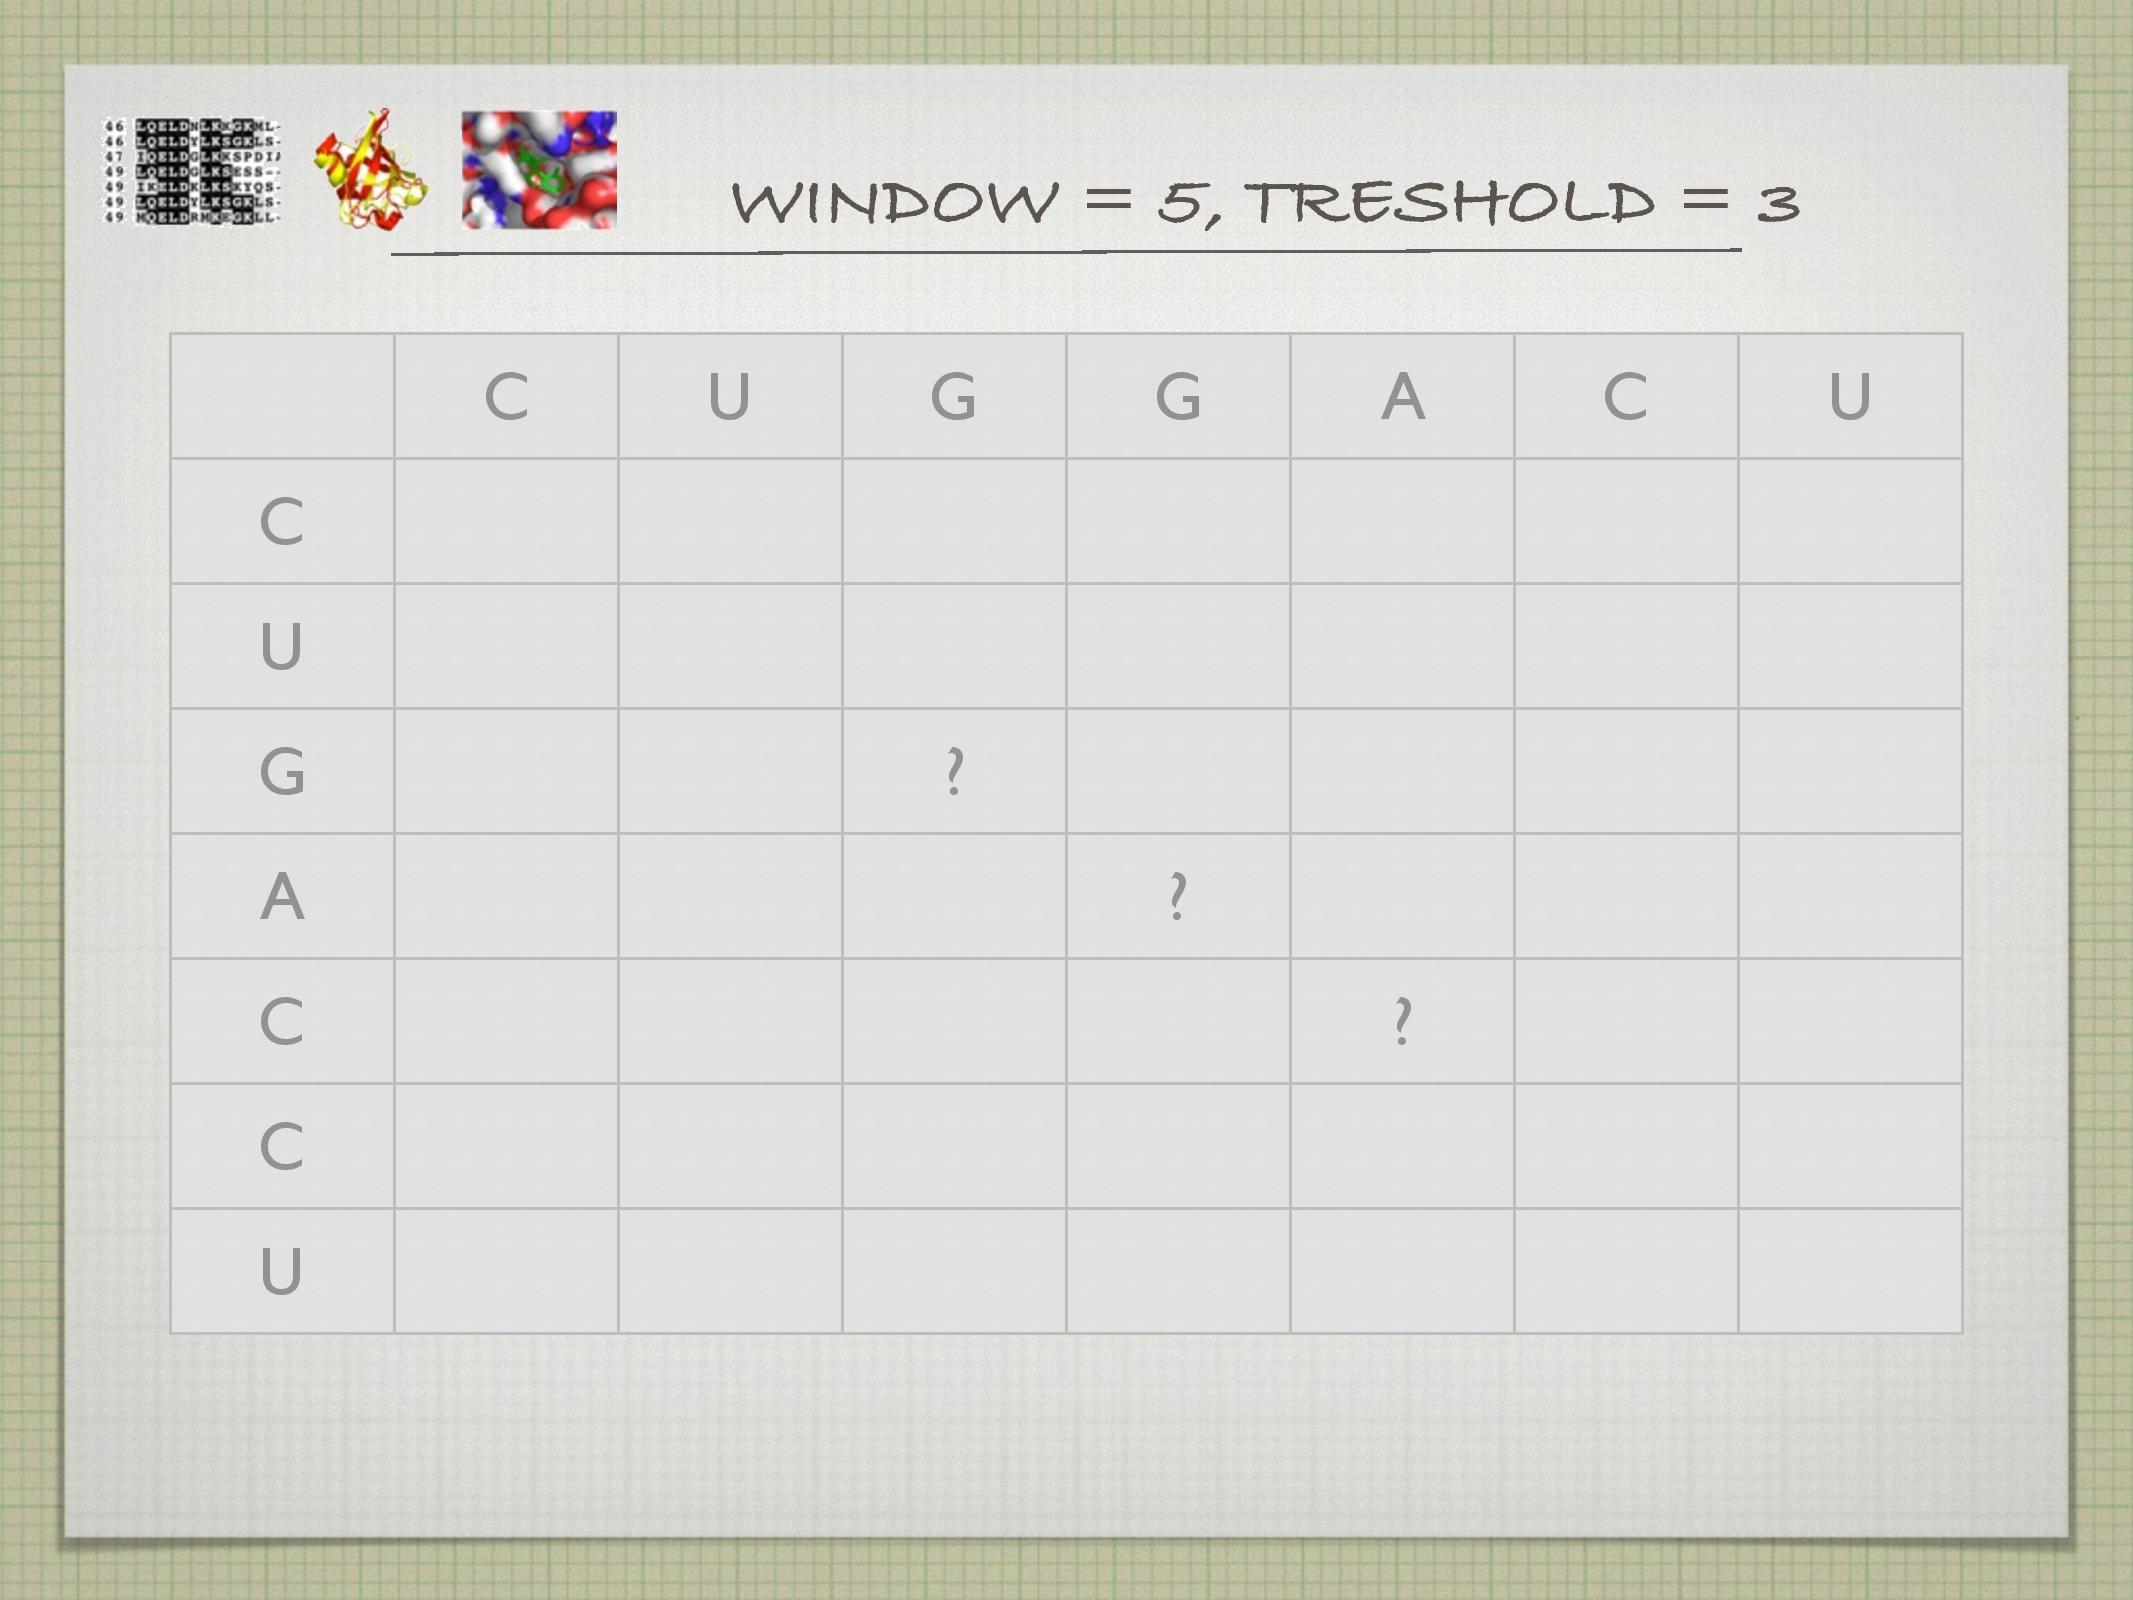
\includegraphics[width=0.85\textwidth]{slides-2/slide-60.jpg}
    \centering
    \label{slides-2-slide-60}
\end{figure}
\begin{figure}
    \caption{Prezentace č. 2, slide č. 61}
    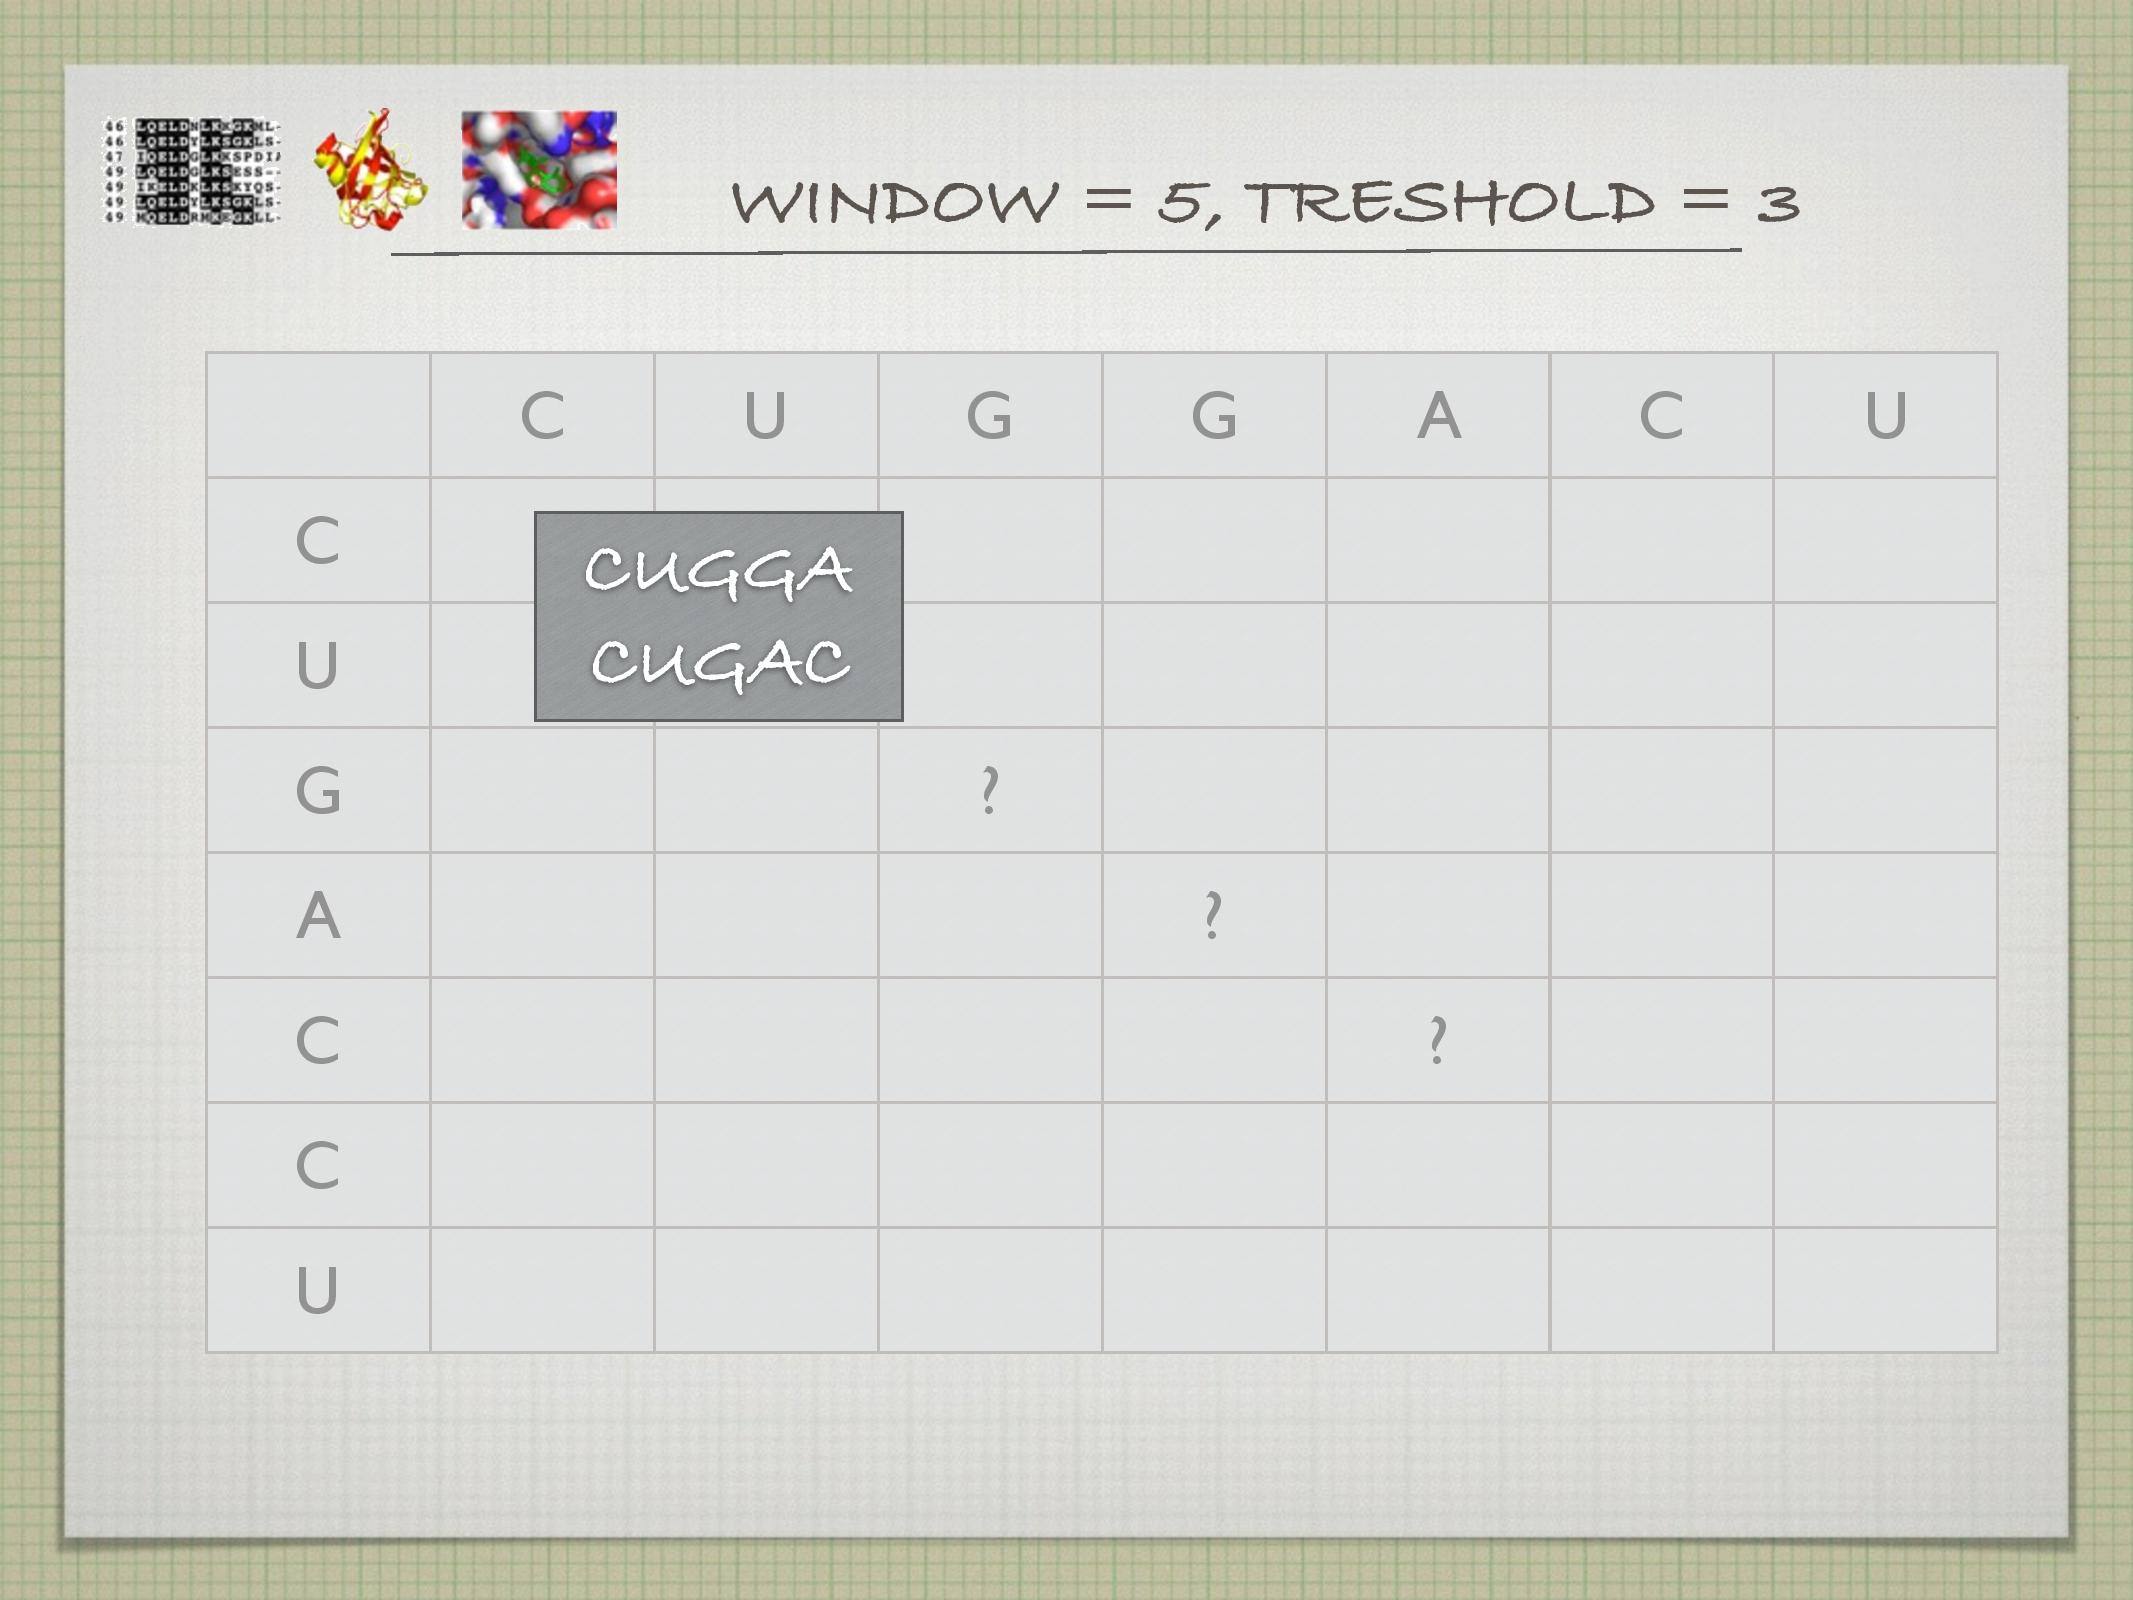
\includegraphics[width=0.85\textwidth]{slides-2/slide-61.jpg}
    \centering
    \label{slides-2-slide-61}
\end{figure}
\begin{figure}
    \caption{Prezentace č. 2, slide č. 62}
    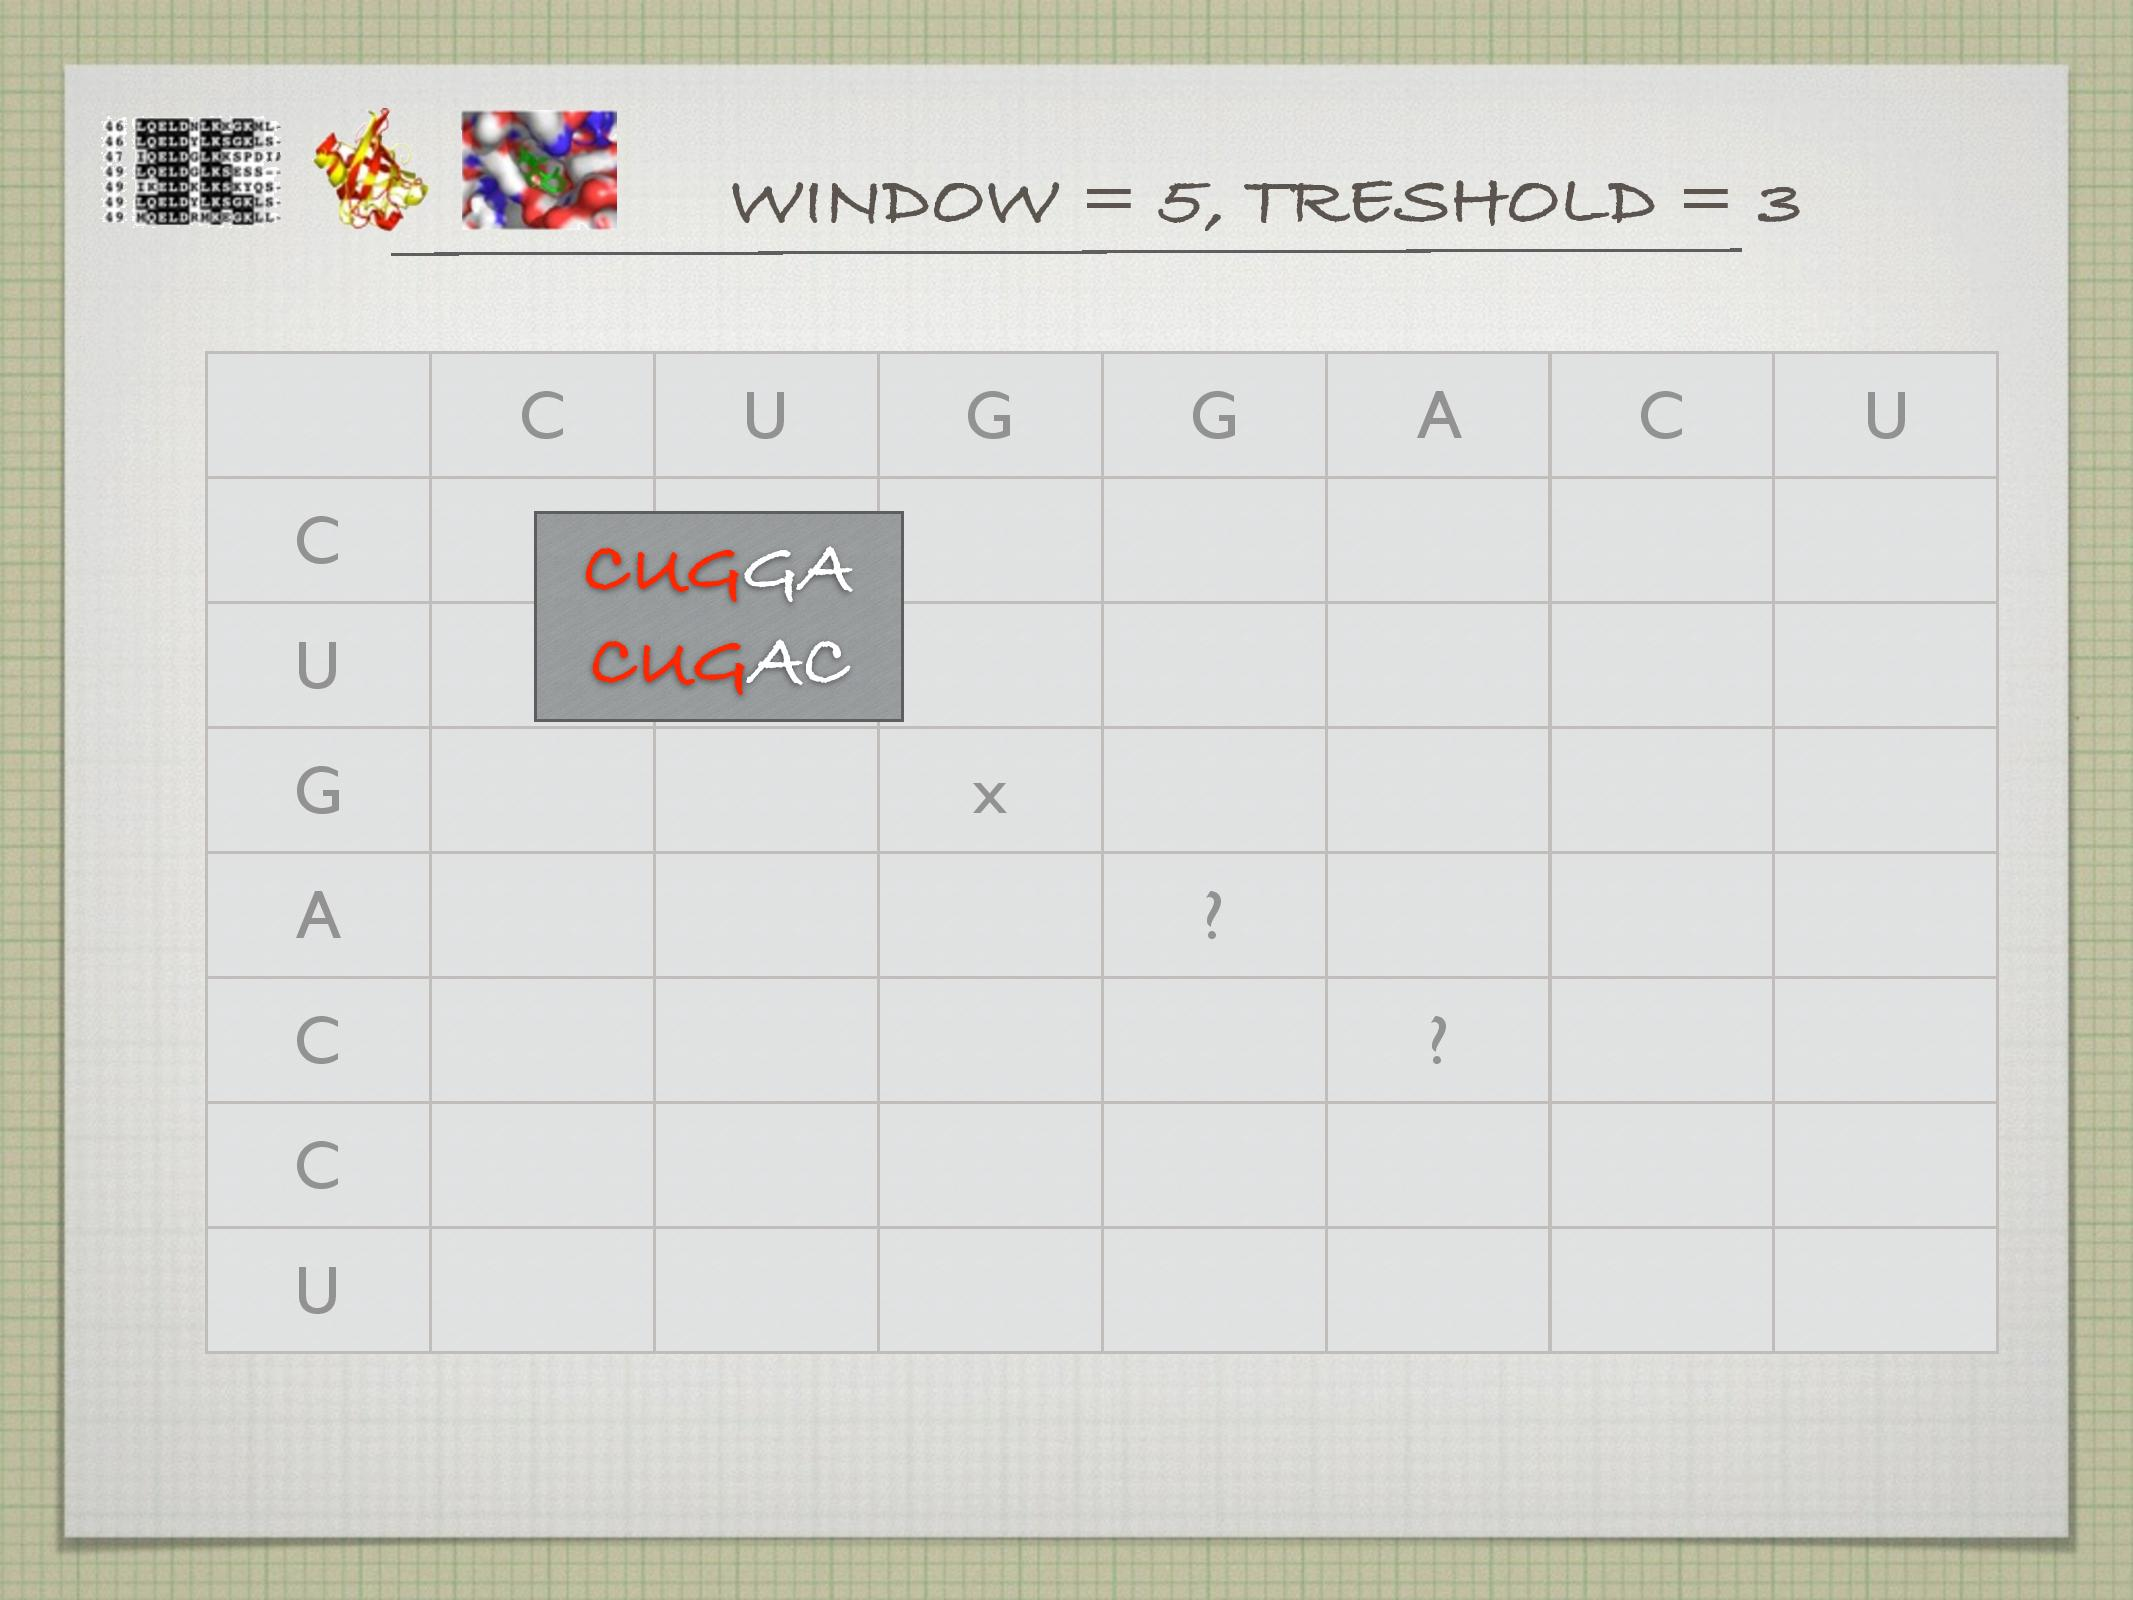
\includegraphics[width=0.85\textwidth]{slides-2/slide-62.jpg}
    \centering
    \label{slides-2-slide-62}
\end{figure}
\begin{figure}
    \caption{Prezentace č. 2, slide č. 63}
    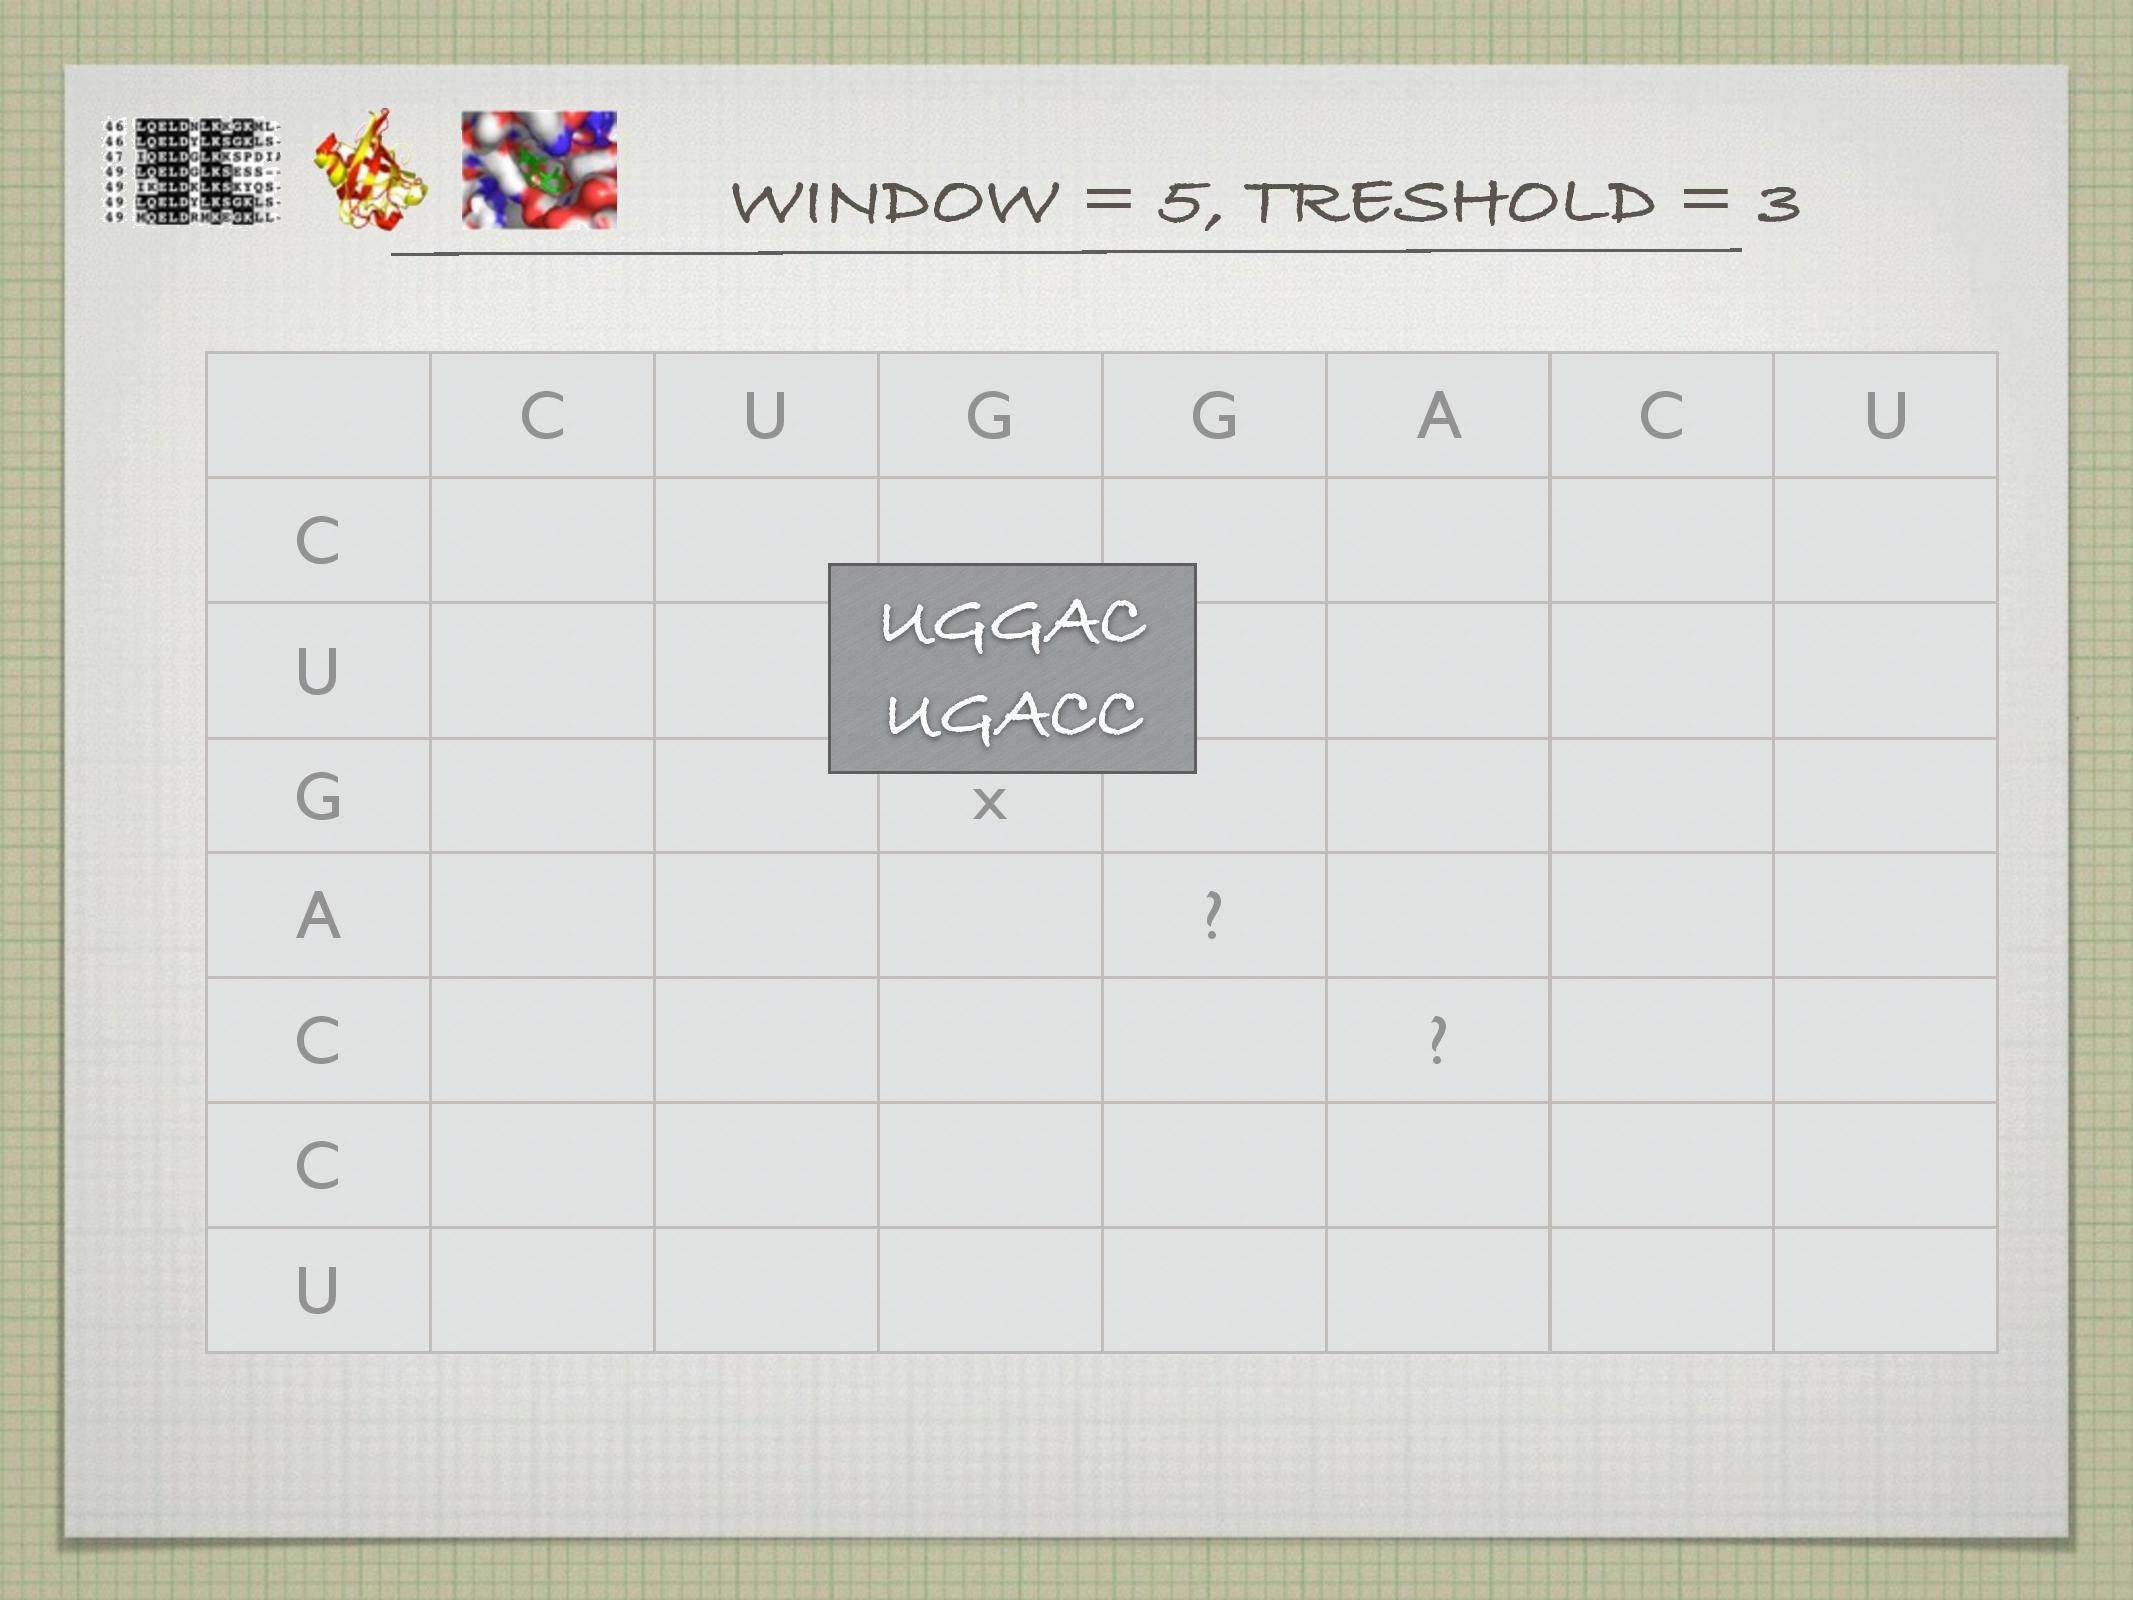
\includegraphics[width=0.85\textwidth]{slides-2/slide-63.jpg}
    \centering
    \label{slides-2-slide-63}
\end{figure}
\begin{figure}
    \caption{Prezentace č. 2, slide č. 64}
    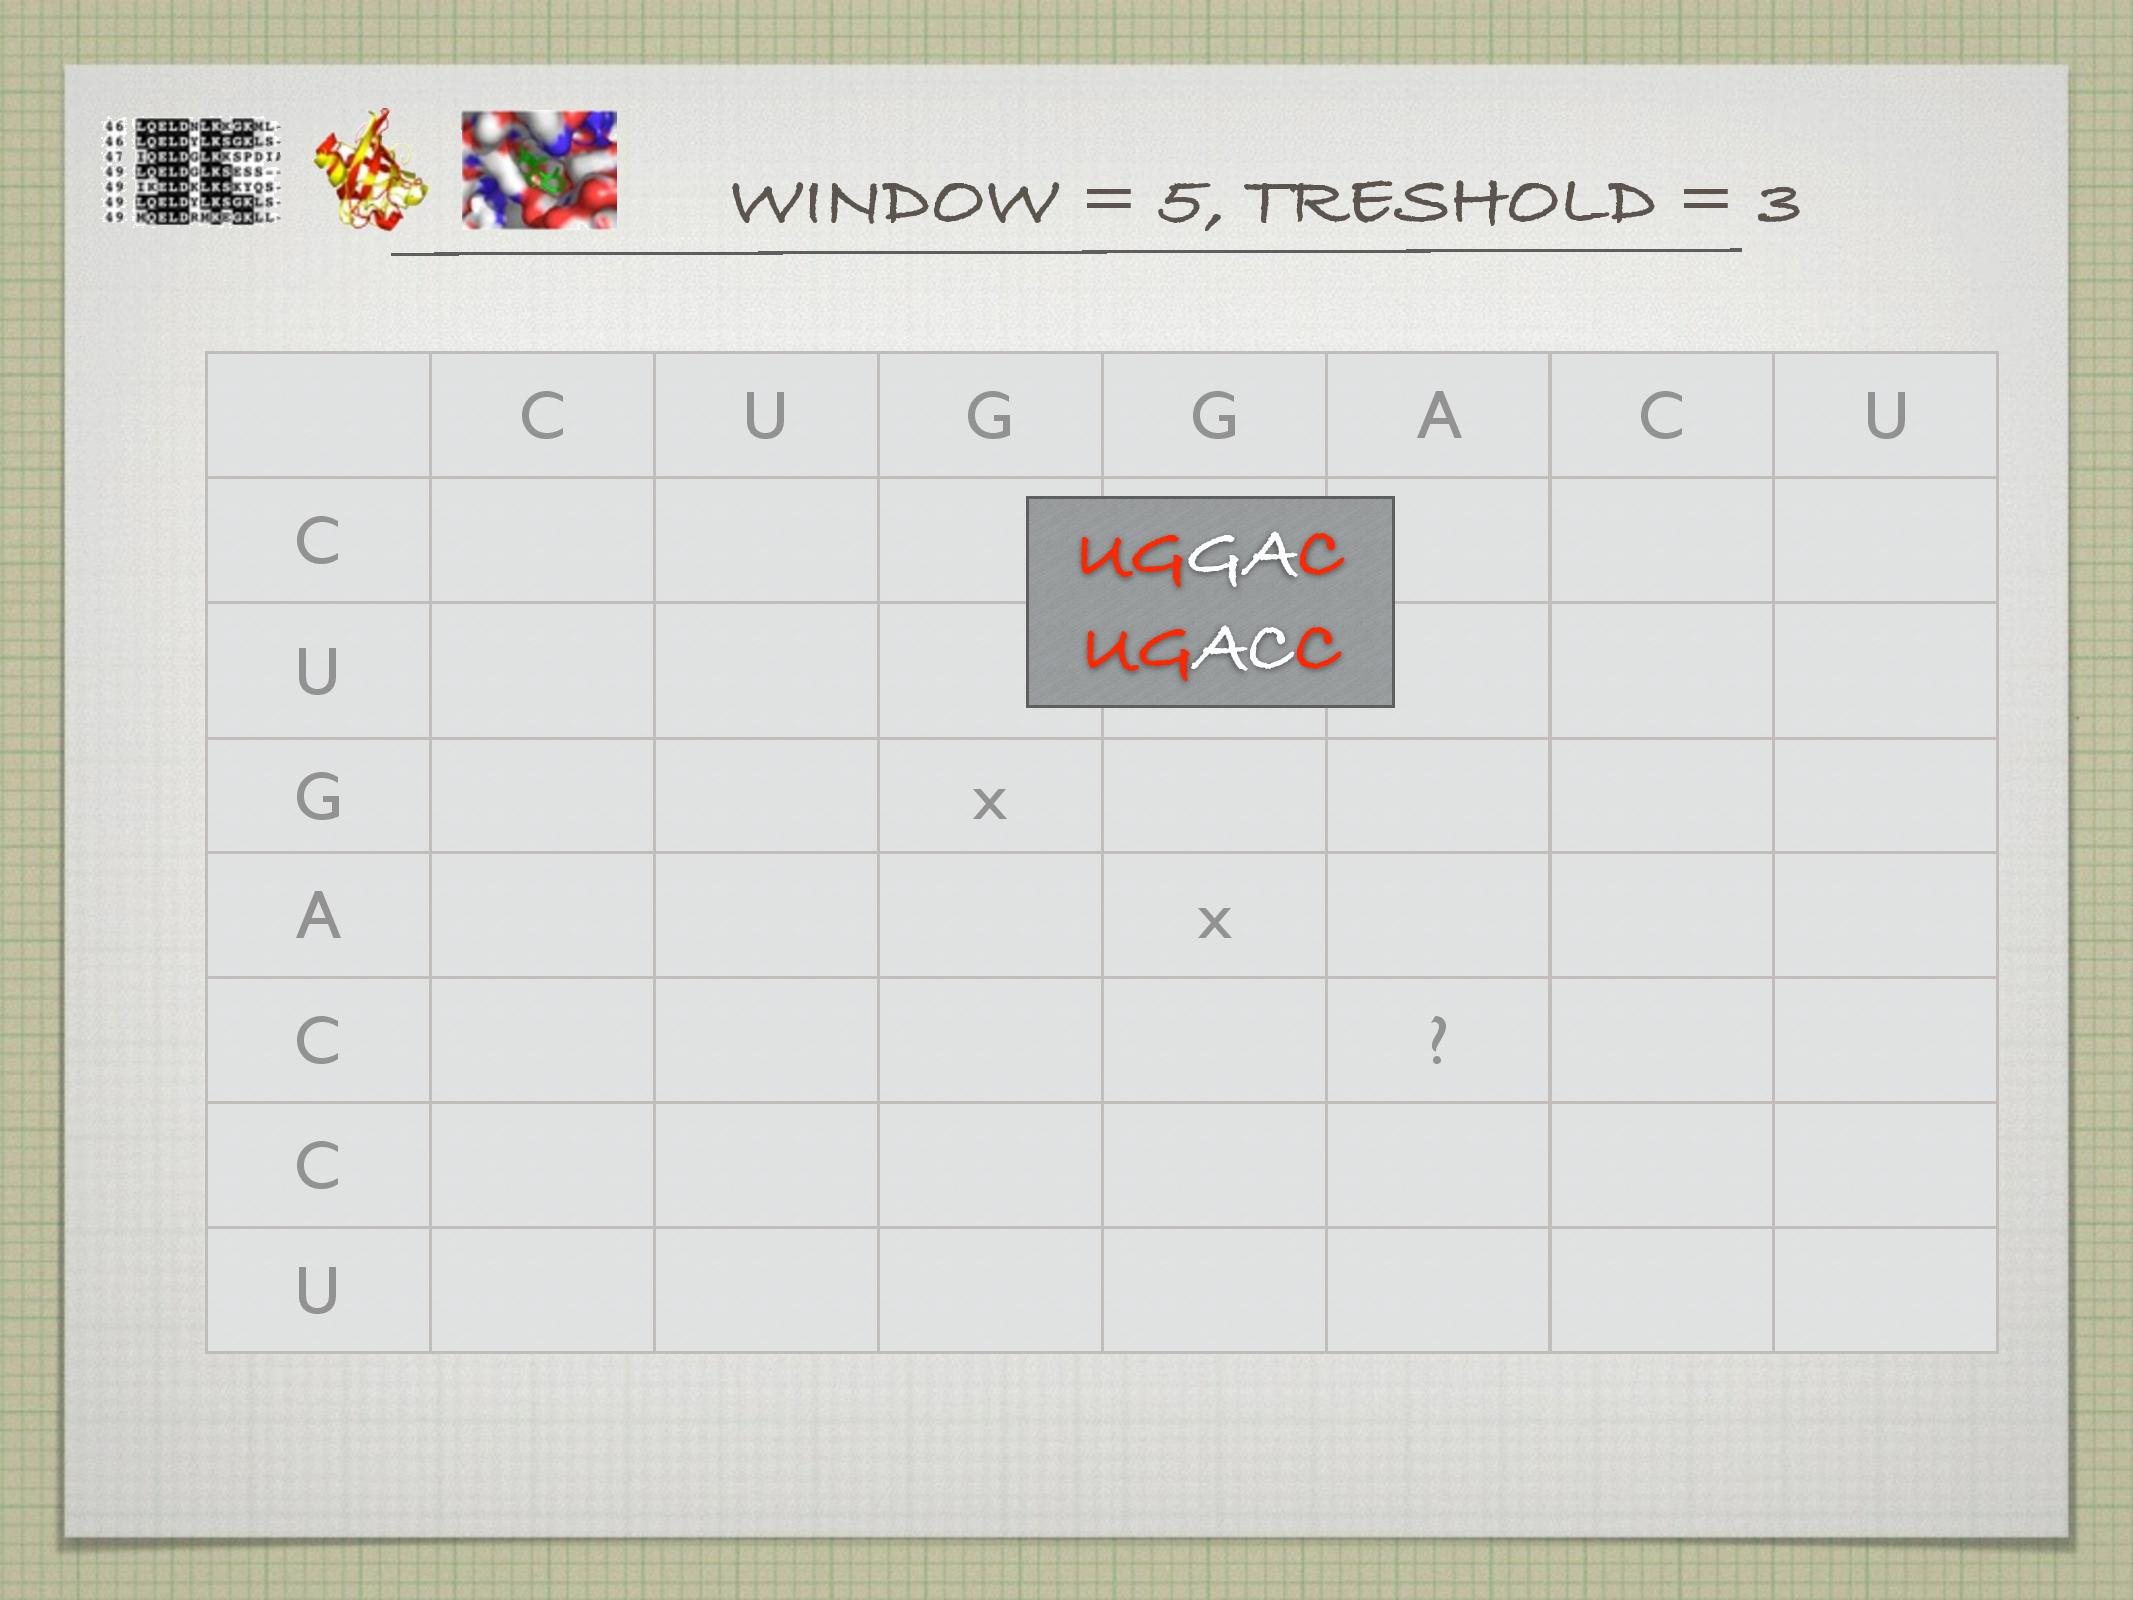
\includegraphics[width=0.85\textwidth]{slides-2/slide-64.jpg}
    \centering
    \label{slides-2-slide-64}
\end{figure}

\begin{figure}
    \caption{Prezentace č. 2, slide č. 67}
    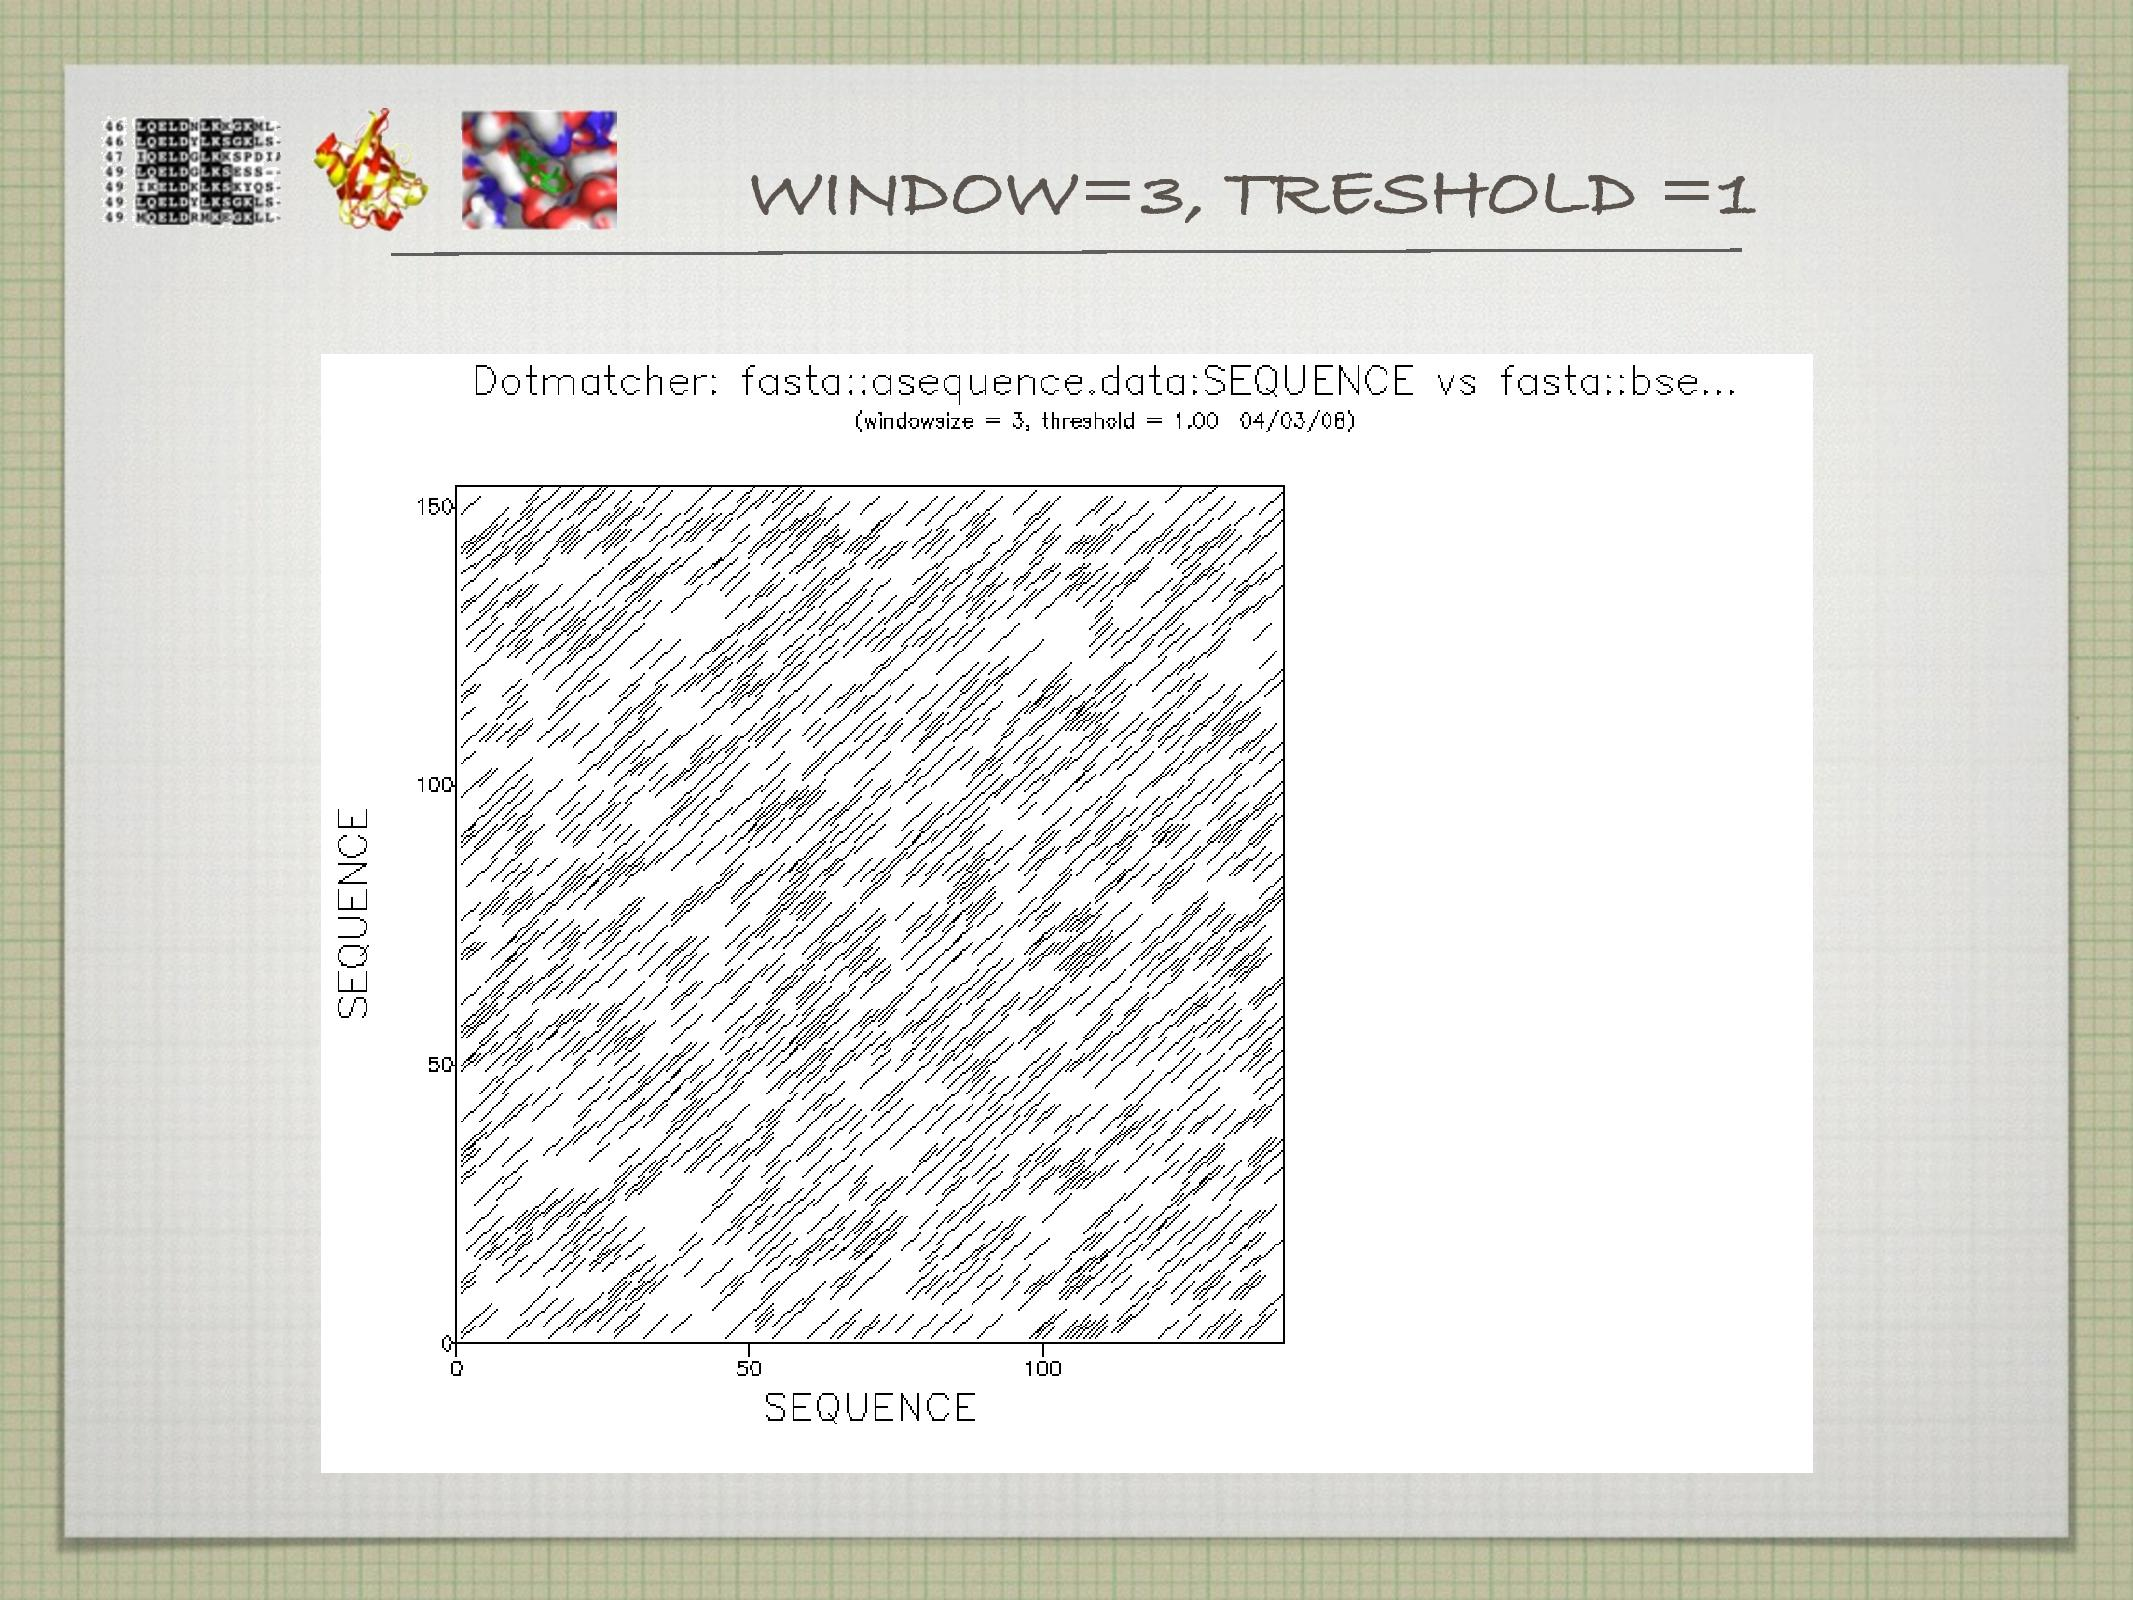
\includegraphics[width=0.85\textwidth]{slides-2/slide-67.jpg}
    \centering
    \label{slides-2-slide-67}
\end{figure}
\begin{figure}
    \caption{Prezentace č. 2, slide č. 68}
    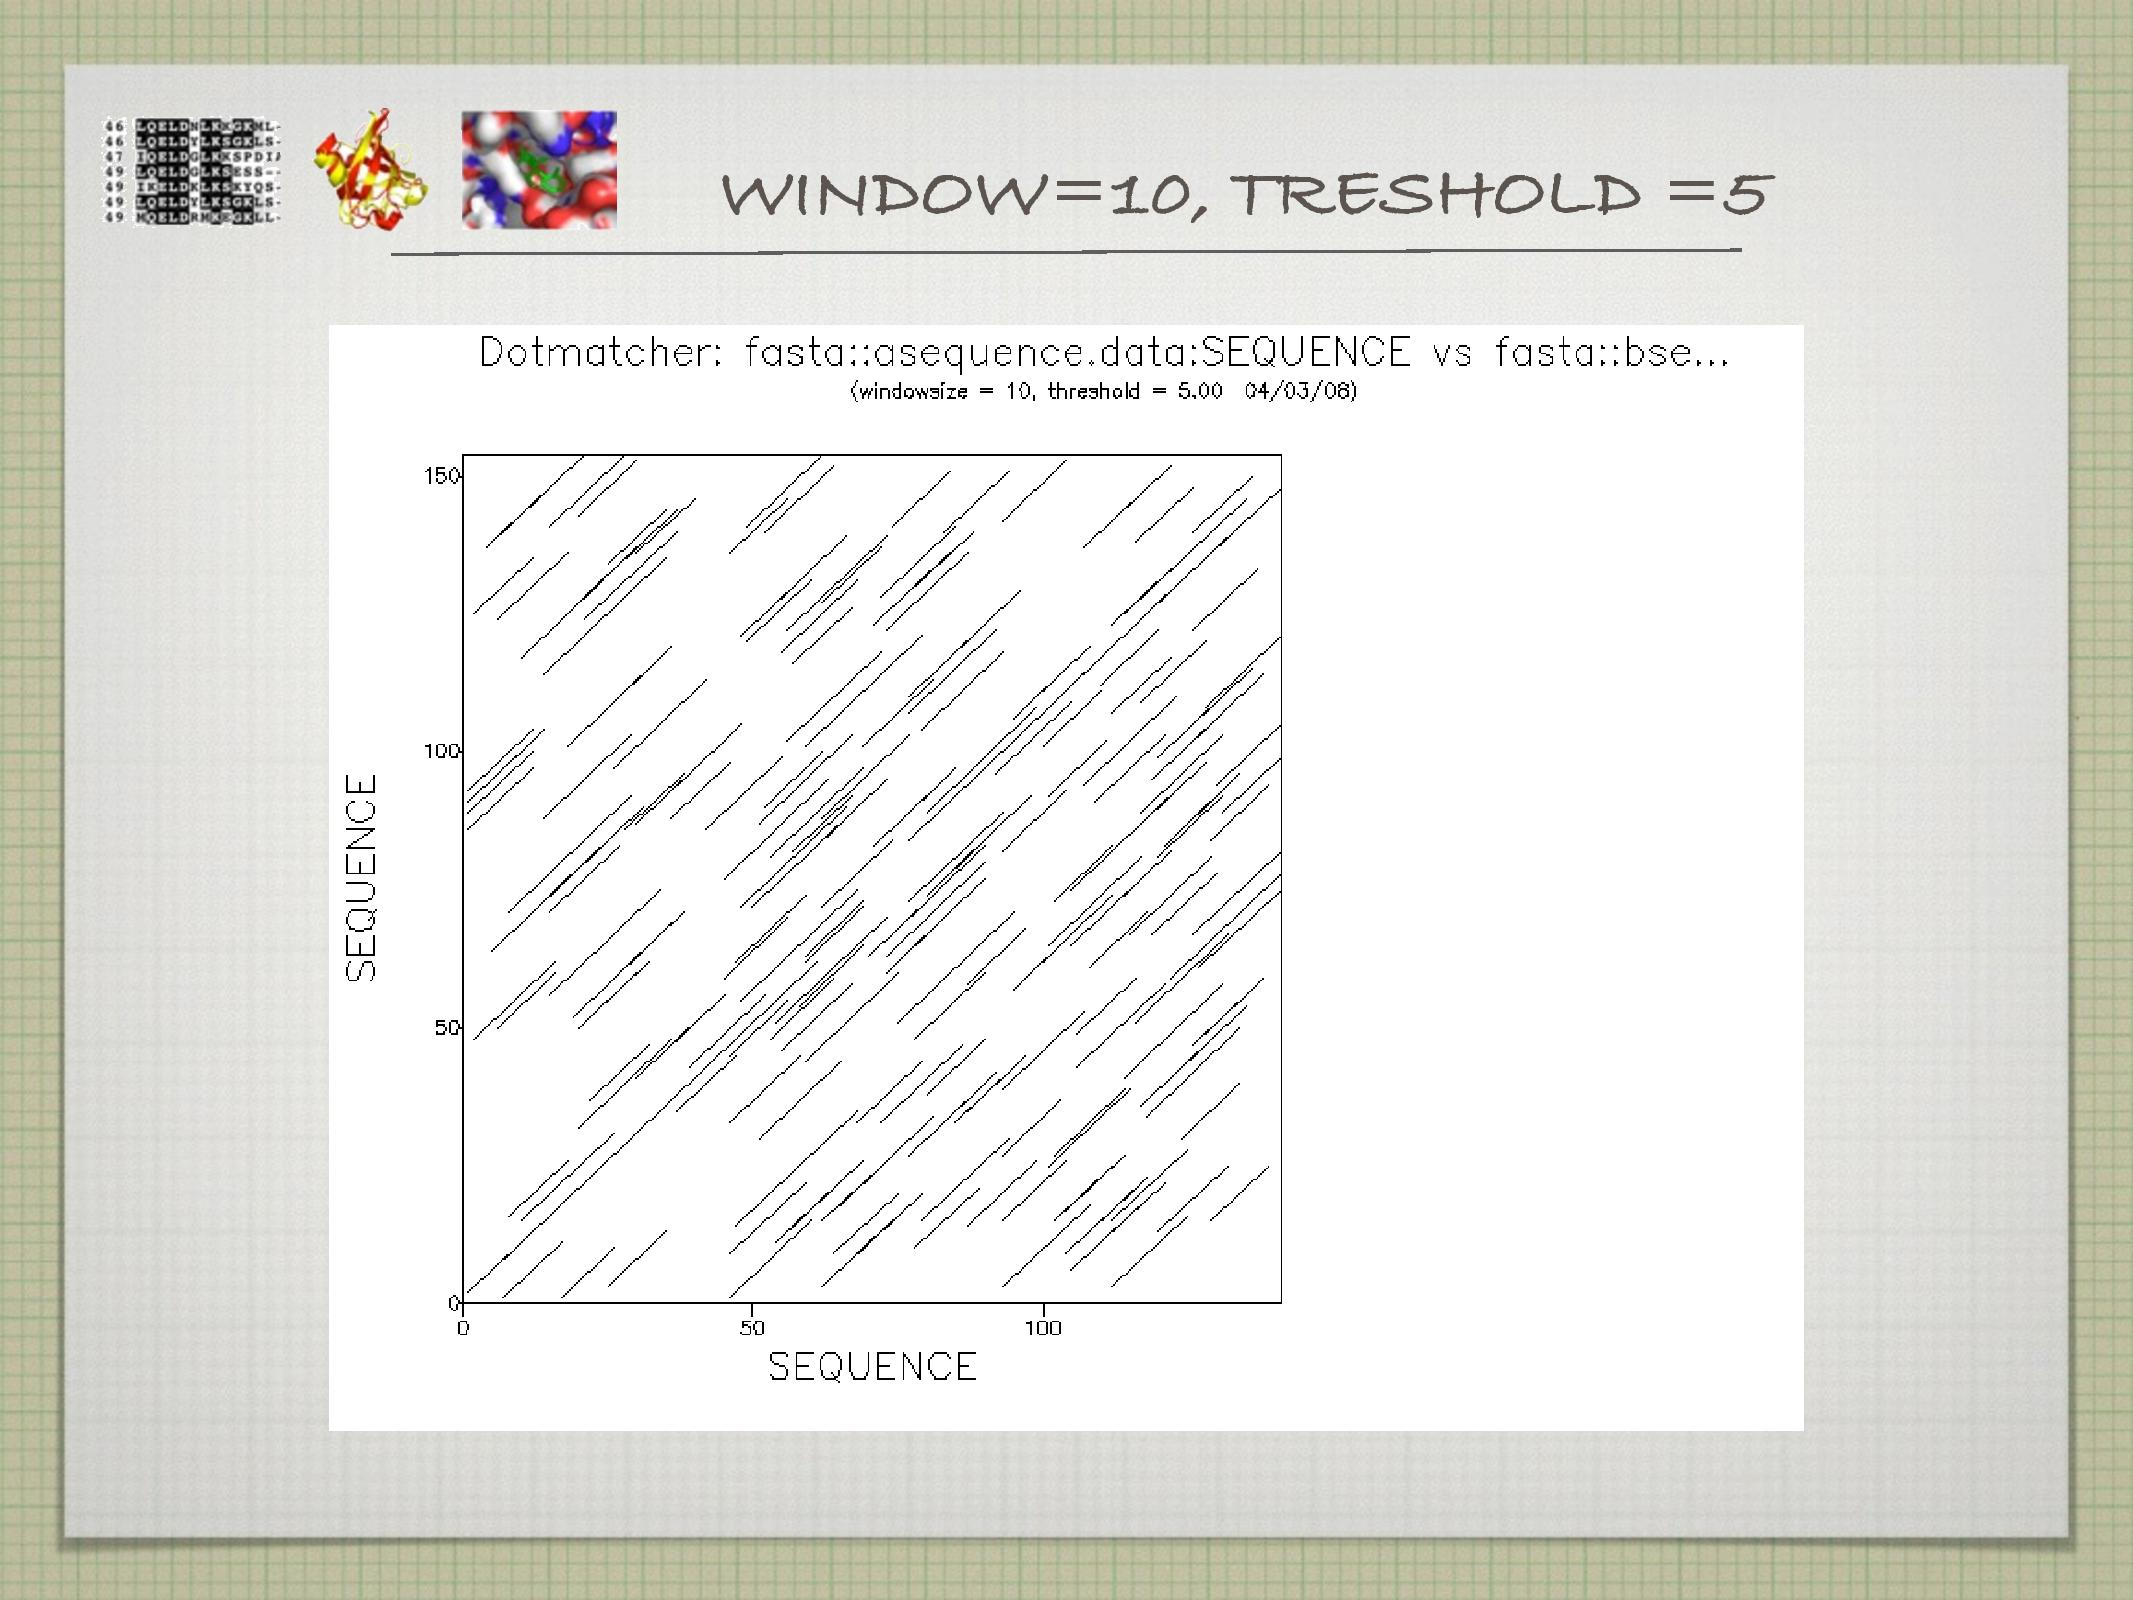
\includegraphics[width=0.85\textwidth]{slides-2/slide-68.jpg}
    \centering
    \label{slides-2-slide-68}
\end{figure}
\begin{figure}
    \caption{Prezentace č. 2, slide č. 69}
    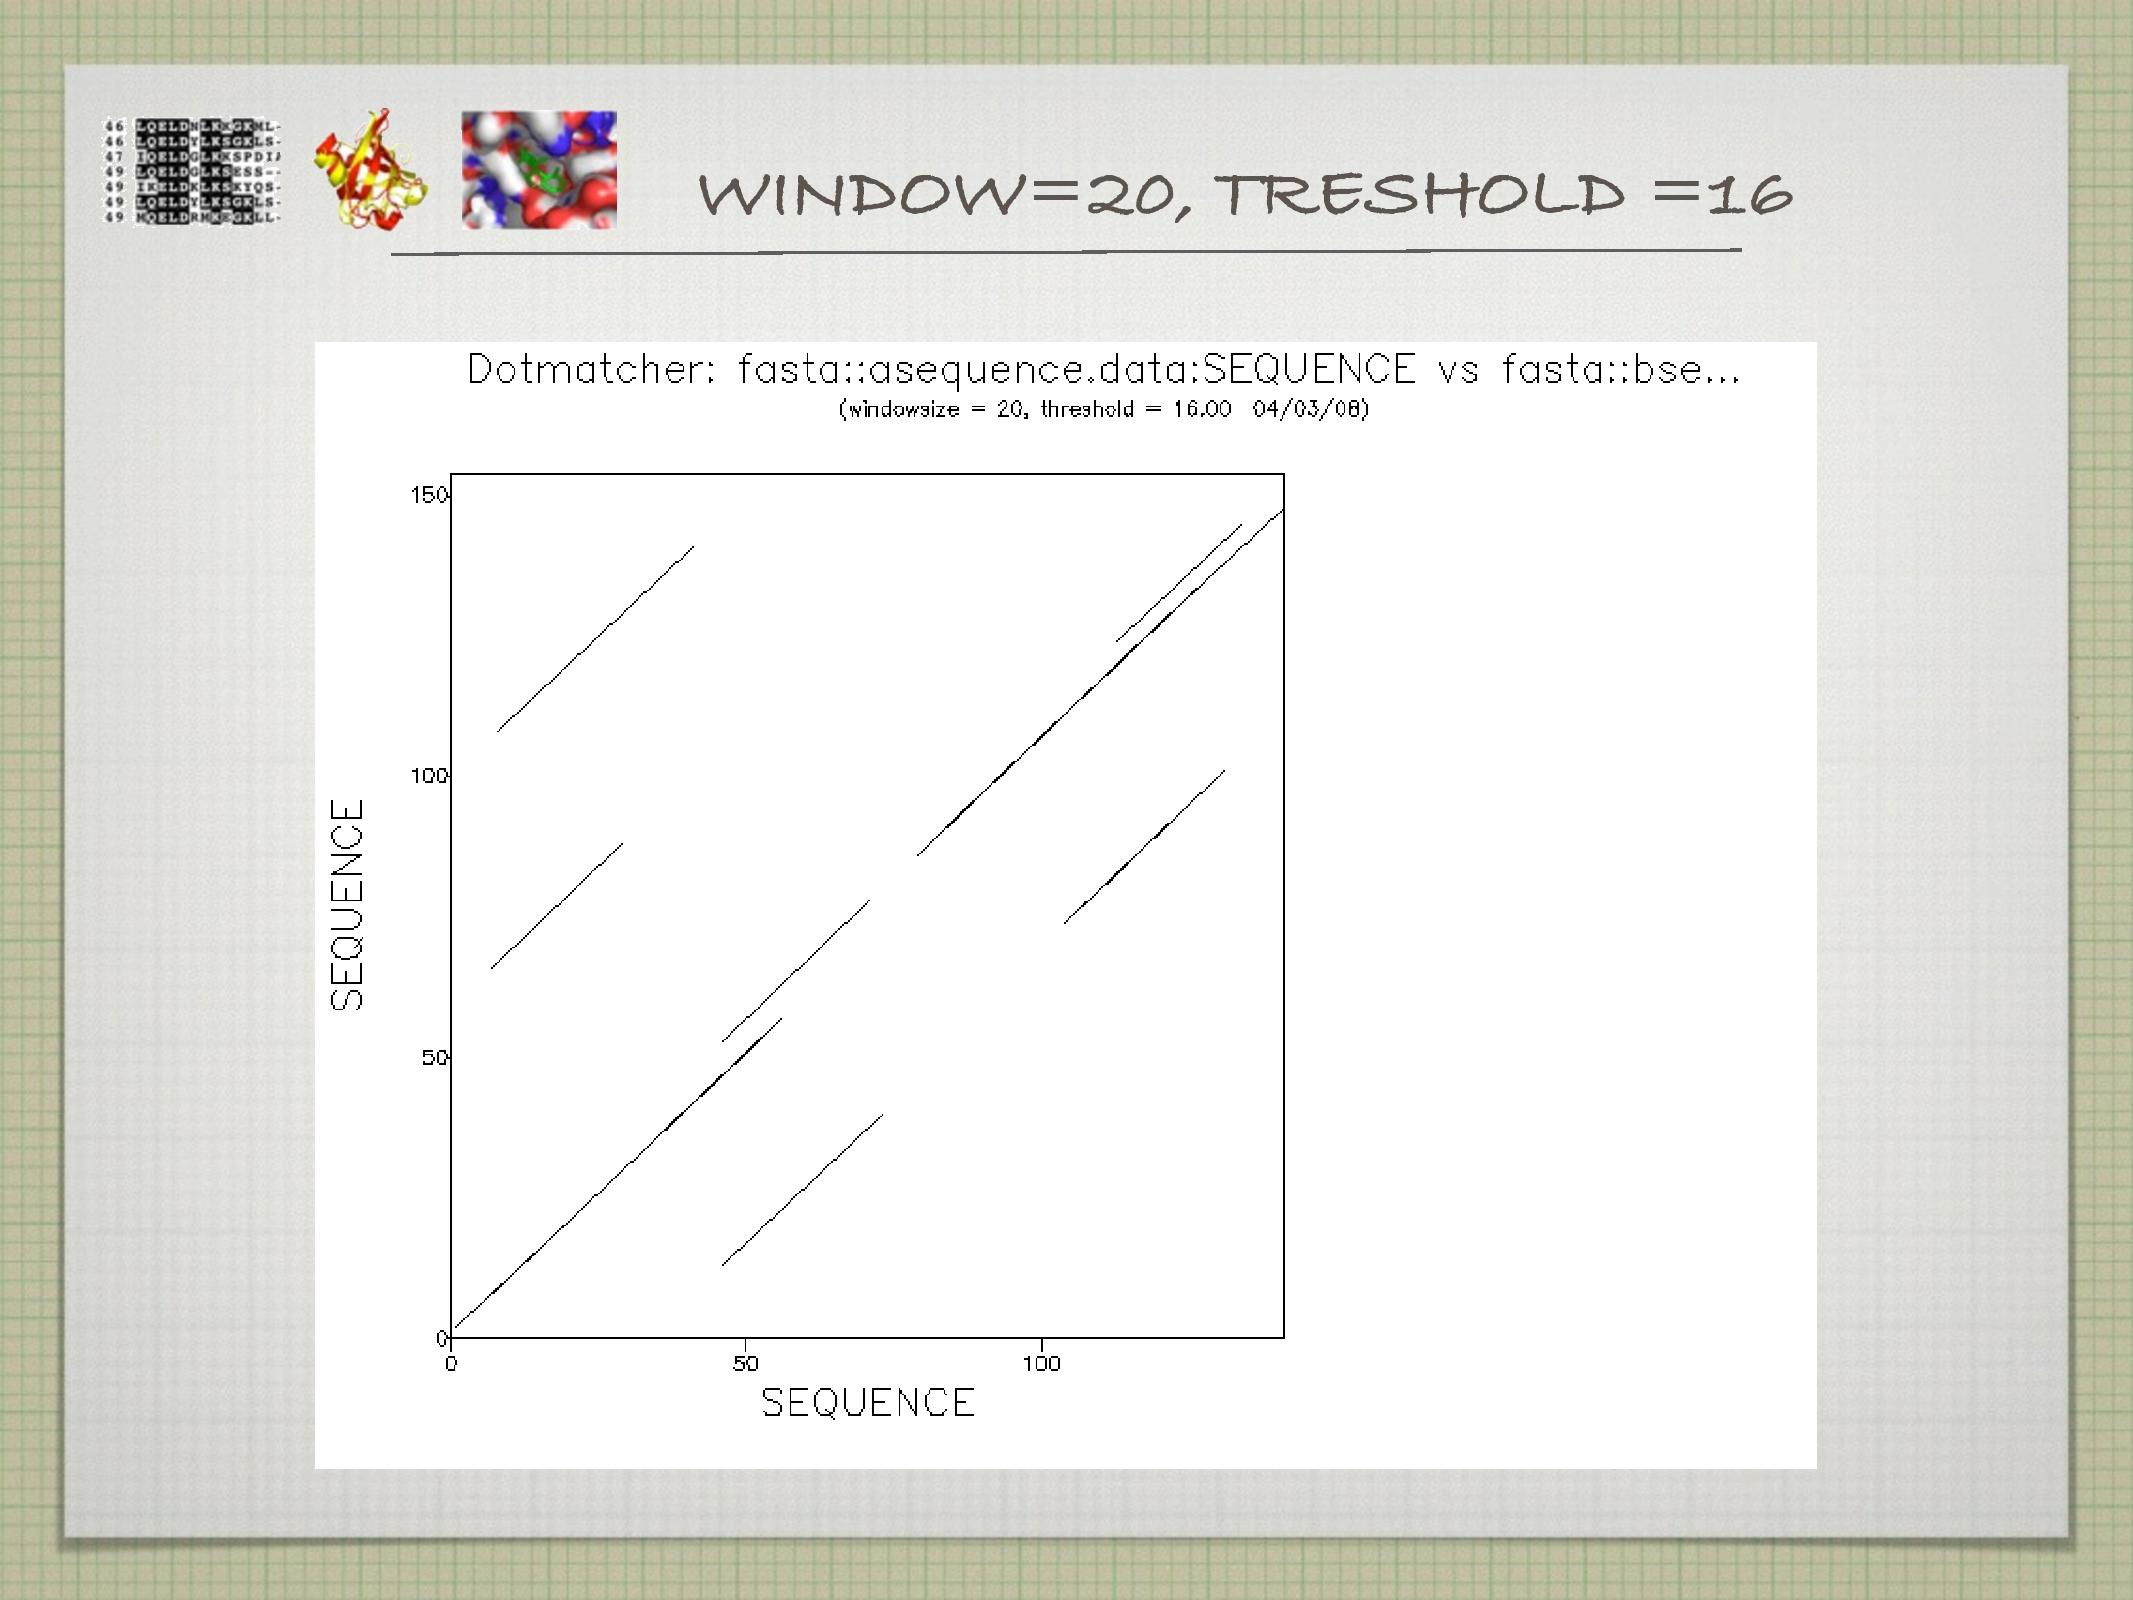
\includegraphics[width=0.85\textwidth]{slides-2/slide-69.jpg}
    \centering
    \label{slides-2-slide-69}
\end{figure}

\paragraph{Slabé stránky}
\begin{itemize}[nosep]
    \item neumí rekonstruovat evoluci (odhalovat homologii atp.)
    \item generuje příliš mnoho signálu, velký šum
\begin{itemize}[nosep]
    \item toto se často "řeší" tak, že se koukáme hned na několik nukleotidů za sebou, a křížek v daném políčku uděláme pouze tehdy, když v tomto našem \emph{klouzavém okně} je více než \(k\) shod
\end{itemize}

    \item ukazuje i náhodné podobnosti
\end{itemize}



V praxi se často používá \textbf{self-dotplot}, tedy dotplot, kde je sekvence srovnávána sama se sebou. Ten opět vyhledává symetrické úseky, repetice, odhaluje místa s nízkou komplexitou a palidromy.

\section{Pairwise sequence alignment} \label{Pairwise sequence alignment}


\emph{Může samozřejmě probíhat i na DNA, pro jednoduchost jej ale popíšeme pouze na proteinech. Pro DNA funguje analogicky.}

Předpokládáme, že sekvence A a B mají společného předka. Poté, když je srovnáme (naalignujeme) "pod sebe", můžeme na každém jednotlivém místě pozorovat následující:
\begin{itemize}[nosep]
    \item \textbf{shoda}: AK v A i v B jsou na daném místě stejné
    \item \textbf{neshoda}: AK v A je na daném místě odlišná od AK v B
    \item \textbf{mezera} (gap): v jedné ze sekvencí došlo při vývoji od společného předka k inzerci nebo deleci
\end{itemize}



\mybox{META}{Gap (mezera v sekvenci při procesu alignmentu) se Švédsky řekne \emph{lucka}.}


Proces alignmentu je vlastně proces umisťování mezer a pozorování toho, jak si poté dvě sekvence navzájem odpovídají. Příklad alignmentu:
\begin{lstlisting}
VLSEGKTEAPV[...]
|||..    ||
VLSPA----PV[...]\end{lstlisting}


Toto je další příklad alignmentu těchto sekvencí; tentokrát dosti nepovedeného:
\begin{lstlisting}
---VLSEGKTEA--PV[...]
   .  ..
V-LS--PA----PV--[...]\end{lstlisting}


Substituce jedné AK za jinou je pravděpodobnější než inzerce/delece. V rámci substitucí je pravděpodobnější substituce podobných jednotek (Val <-> Leu, G <-> A) než těch nepodobných (Trp <-> Gly, G <-> C).

\begin{figure}
    \caption{Prezentace č. 2, slide č. 87}
    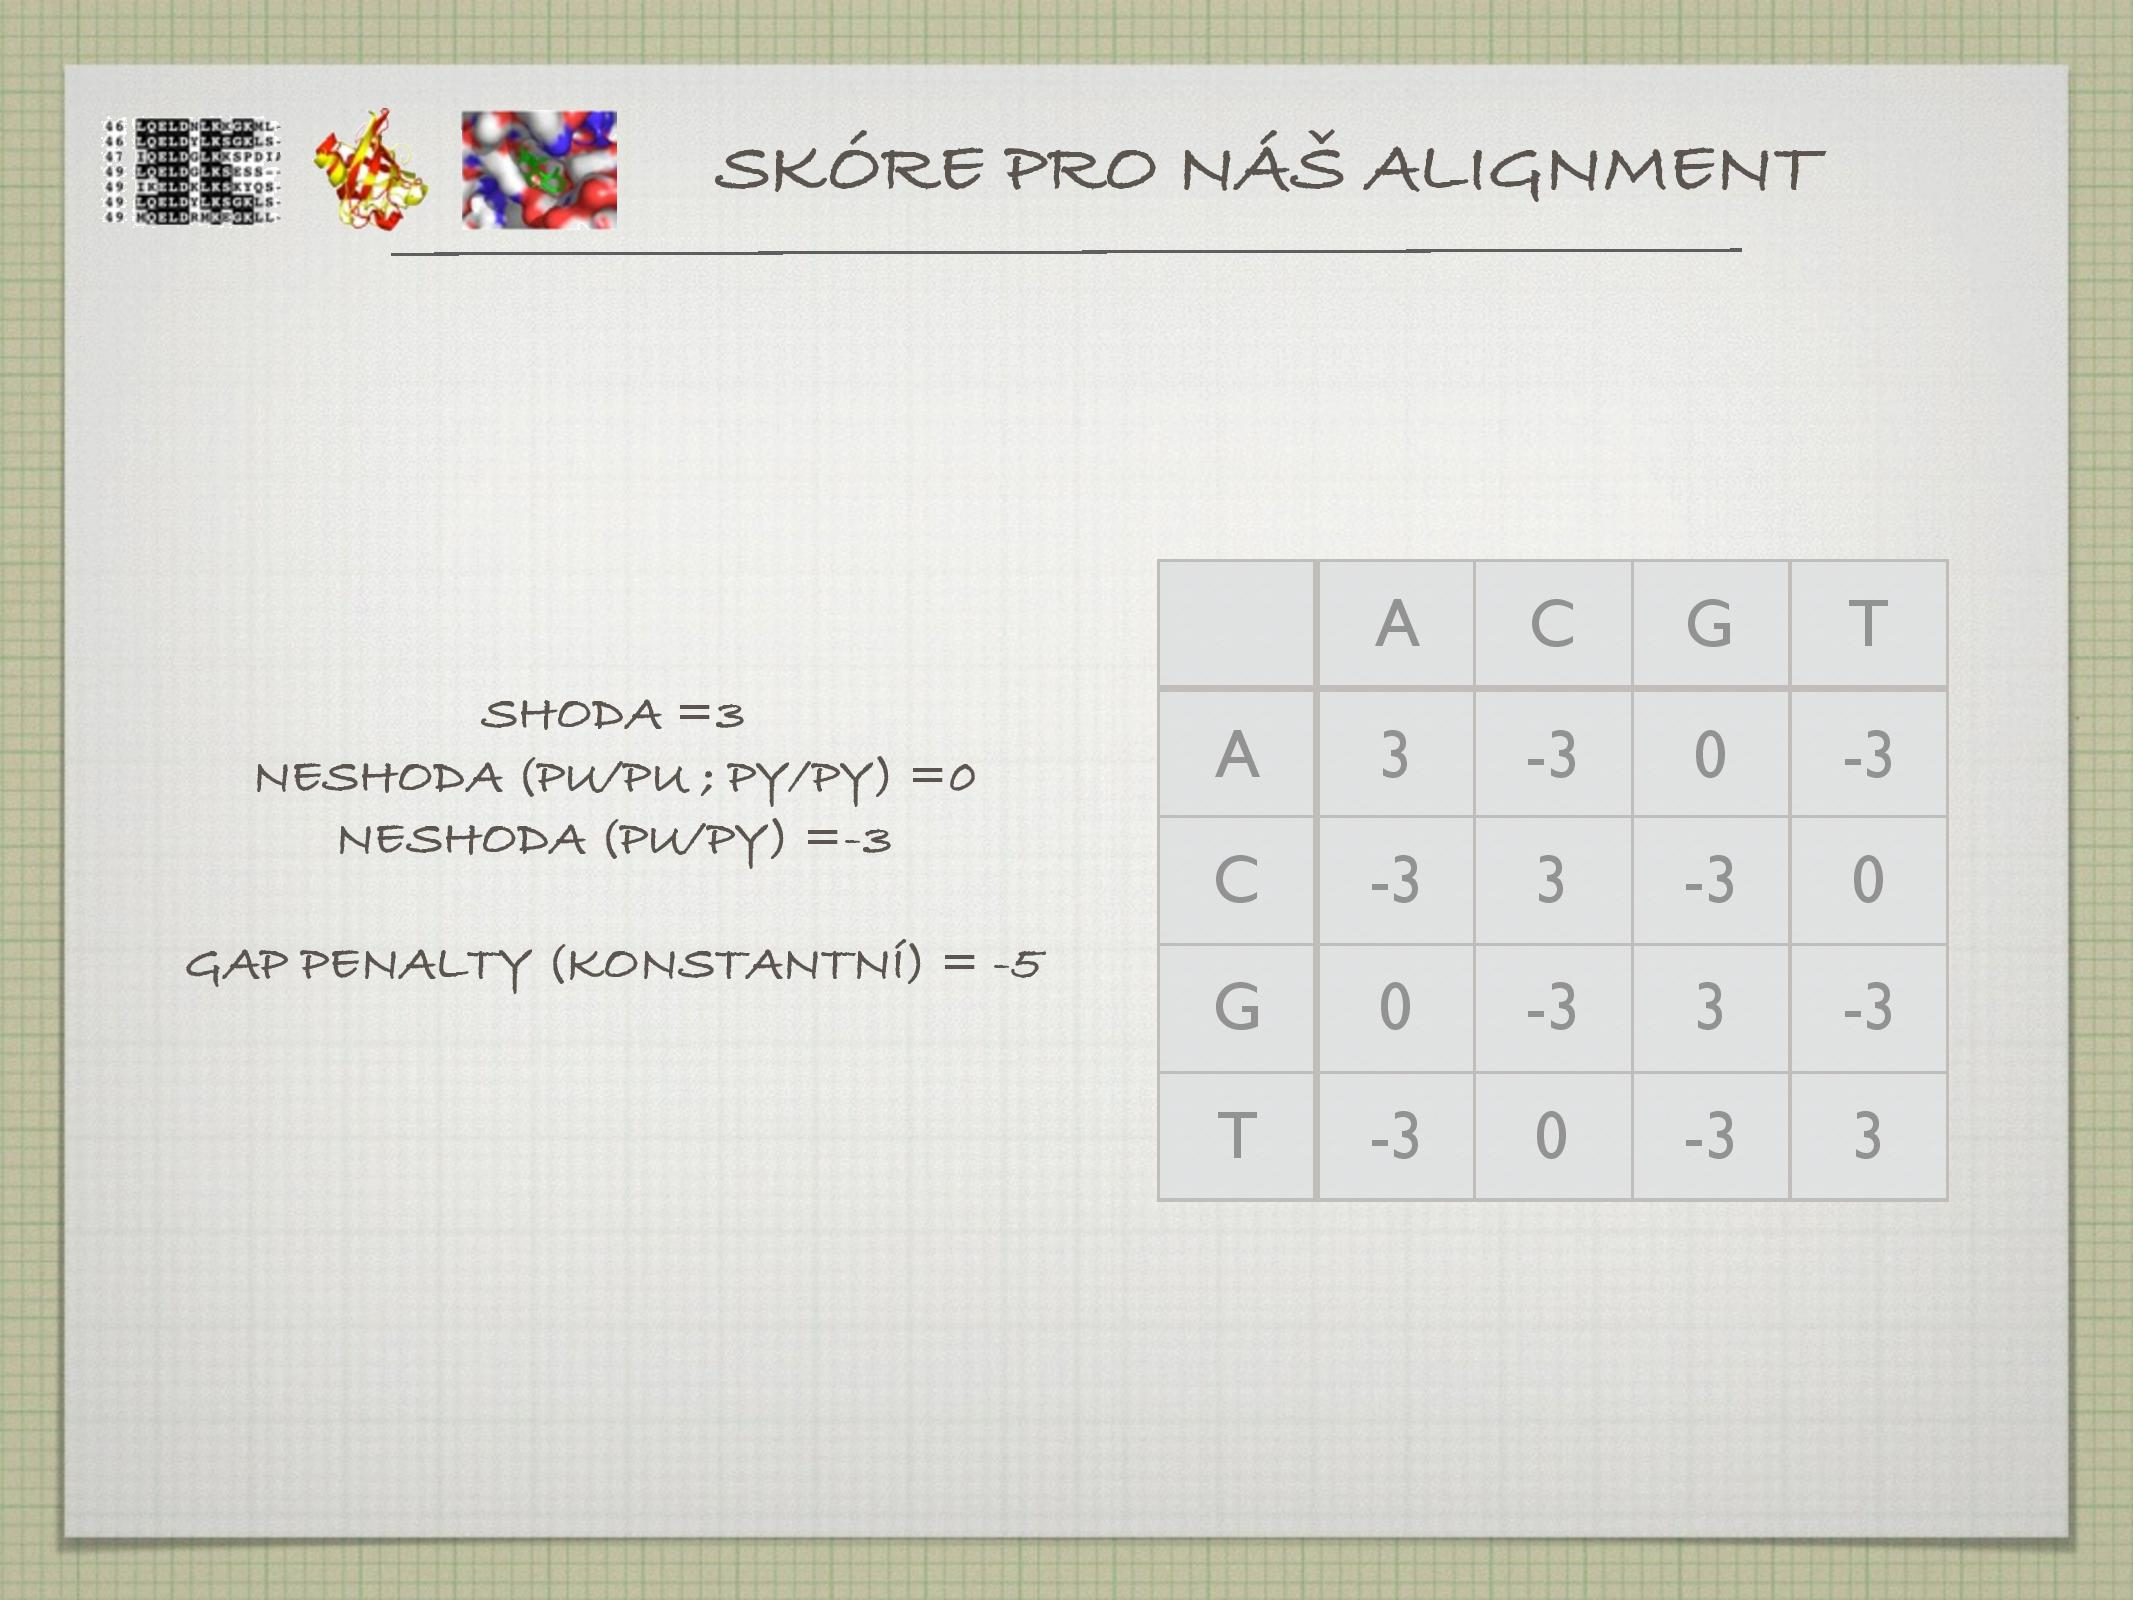
\includegraphics[width=0.85\textwidth]{slides-2/slide-87.jpg}
    \centering
    \label{slides-2-slide-87}
\end{figure}
\begin{figure}
    \caption{Prezentace č. 2, slide č. 97}
    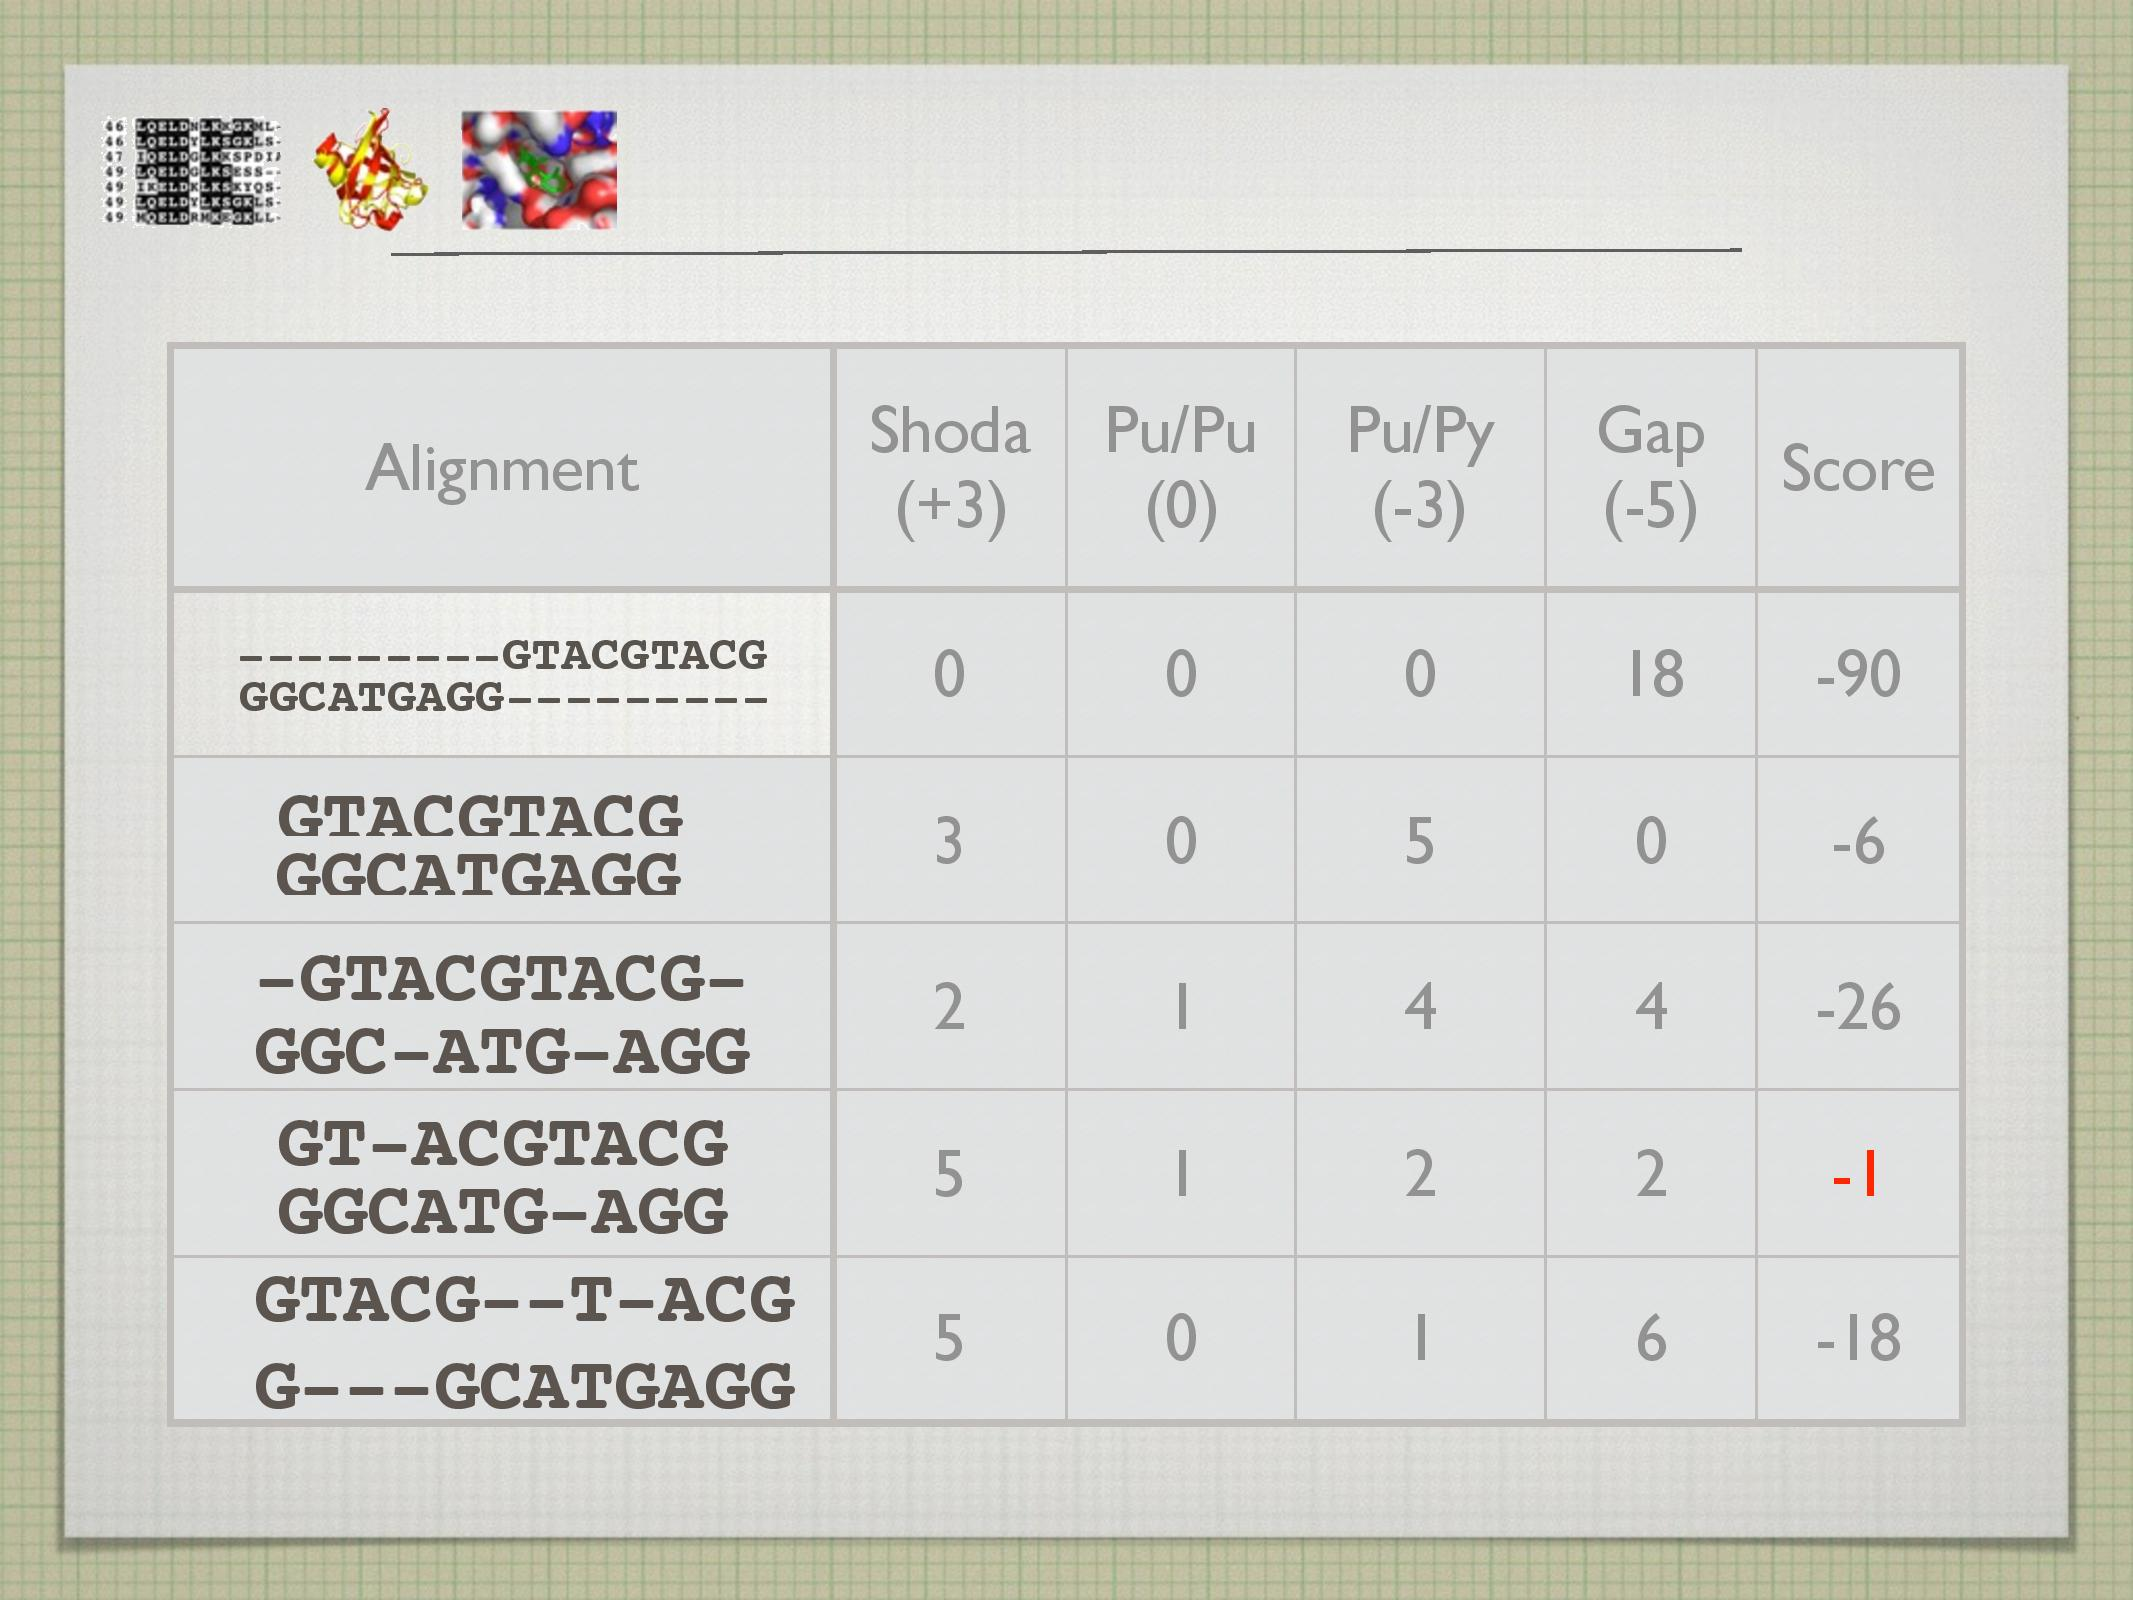
\includegraphics[width=0.85\textwidth]{slides-2/slide-97.jpg}
    \centering
    \label{slides-2-slide-97}
\end{figure}

\paragraph{Měřítko kvality alignmentu}
\begin{itemize}[nosep]
    \item alignmentů je nekonečně mnoho, musíme vybrat ty nejpravděpodobnější, pokud z nich chceme něco vyvozovat (společnou strukturu, funkci atp.)
    \item většinou alignment skórujeme po jednotkách
\begin{itemize}[nosep]
    \item shoda/neshoda jsou za určitý počet bodů (klidně záporných)
    \item mezery jsou za záporné body (tzv. \emph{gap penalty}, GP), většinou za začátek mezery je více záporných bodů než za její rozšíření
\end{itemize}

    \item skóre pro všechny kombinace shod/neshod bývá uloženo v tabulkách
    \item tyto tabulky, společně s určením hodnot gap penalty, velice ovlivňují výsledný (vybraný) alignment
\begin{itemize}[nosep]
    \item z toho plyne snaha o optimalizaci tabulek i GP tak, aby co nejvíce odpovídali biologickým empirickým datům (netvořily nesmyslné alignmenty)
    \item optimální tabulky/GP se liší protein od proteinu
    \item vznikají experimentální variabilní GP založeny na strukturních datech proteinů (v pravidelných sekundárních strukturách je nizší pravděpodobnost výskytu mezery)
\end{itemize}

\end{itemize}



K hledání optimálního (nebo suboptimálního) alignmentu používá algoritmus, který projde mnoho různých možncých alignmentů a vybere z nich ten s nejvyšším skóre dle přidělené skórovací tabulky. Pozor, ani nejlepší alignment nemusí odpovídat reálu.

\subsection{Skórovací tabulky} \label{Skórovací tabulky}


Neboli \textbf{scoring matrices}.

\paragraph{Určení hodnot skóre}
\begin{itemize}[nosep]
    \item skóre původně určeno z fyzikálněchemických, tedy teoretických, vlastností AK
    \item nyní máme mnoho empirickcýh dat, skóre tvoříme na základě nich
\begin{itemize}[nosep]
    \item skóre záměny jedné AK za jinou je tedy postaveno na základě pravděpodobnosti toho, že tato záměna v reálu proběhne, kterou zjistíme z pozorovaných sekvencí
\end{itemize}

\end{itemize}



Tabulky jsou tedy symetrické --- nejsme schopni z empirických dat zjistit, jakým směrem proběhla substituce (pokud máme na daném místě v jedné sekvenci Ile a v druhé Val, nevíme, které AK z těch dvou tam byla původně, a která tam bylo substituována dodatečně).


\begin{figure}
    \caption{Prezentace č. 3, slide č. 26}
    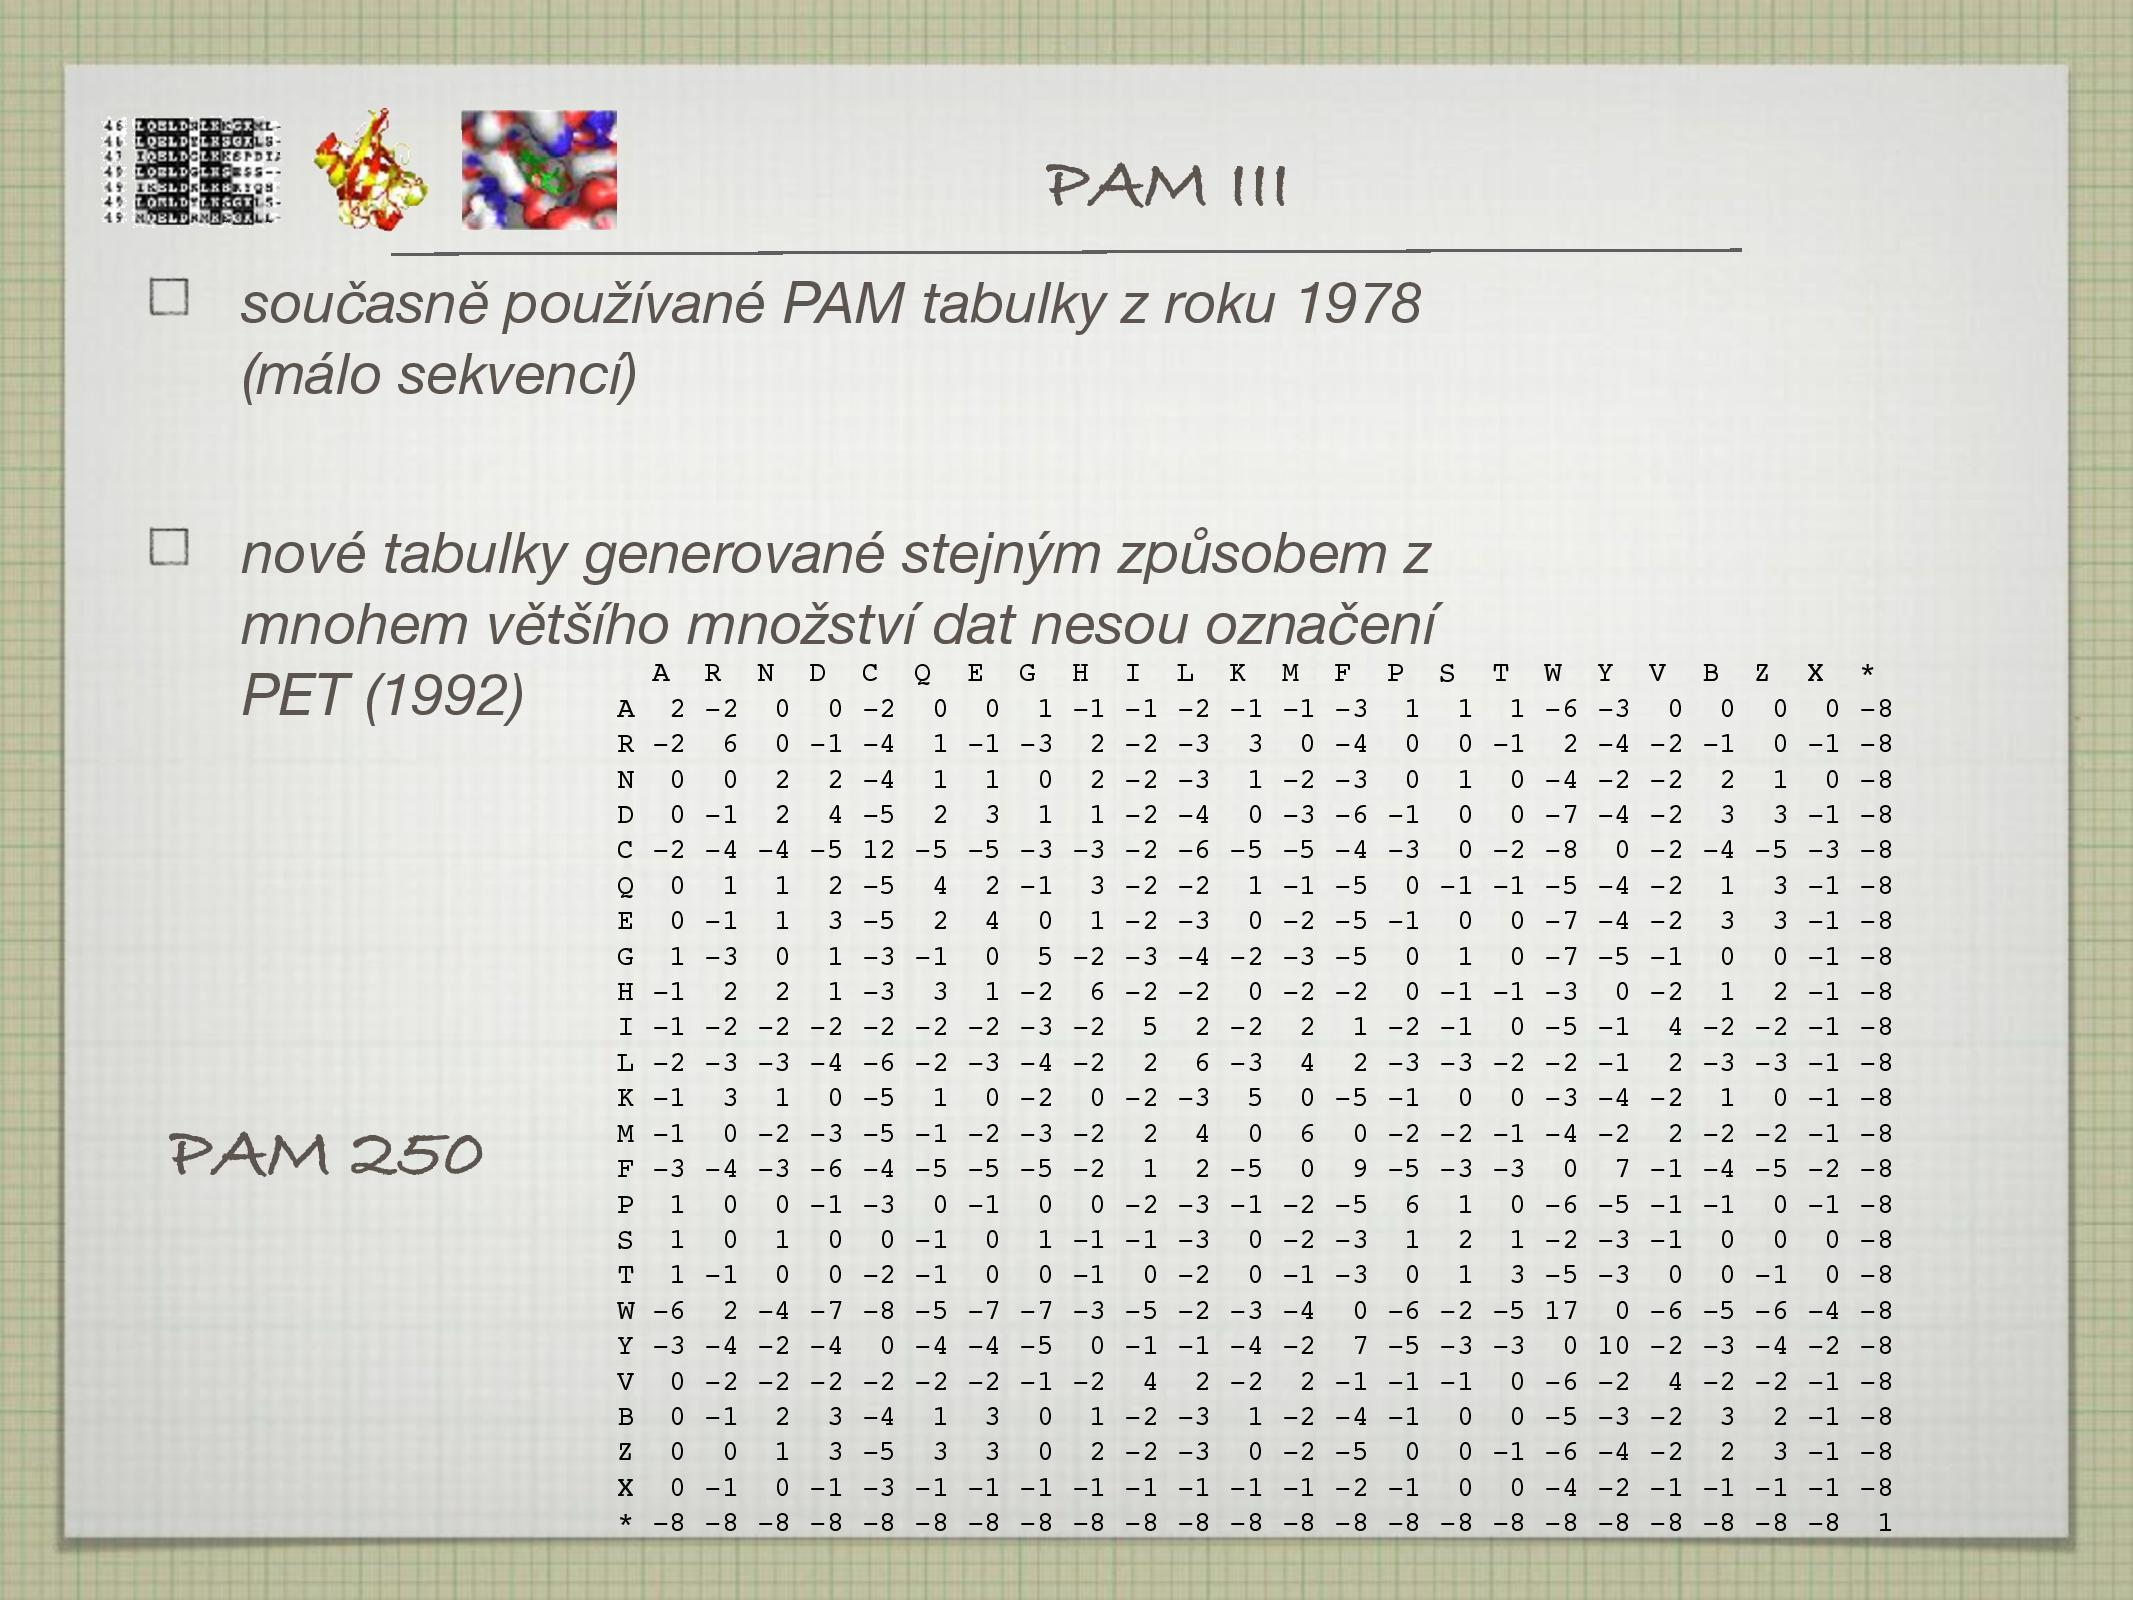
\includegraphics[width=0.85\textwidth]{slides-3/slide-26.jpg}
    \centering
    \label{slides-3-slide-26}
\end{figure}
\begin{figure}
    \caption{Prezentace č. 3, slide č. 23}
    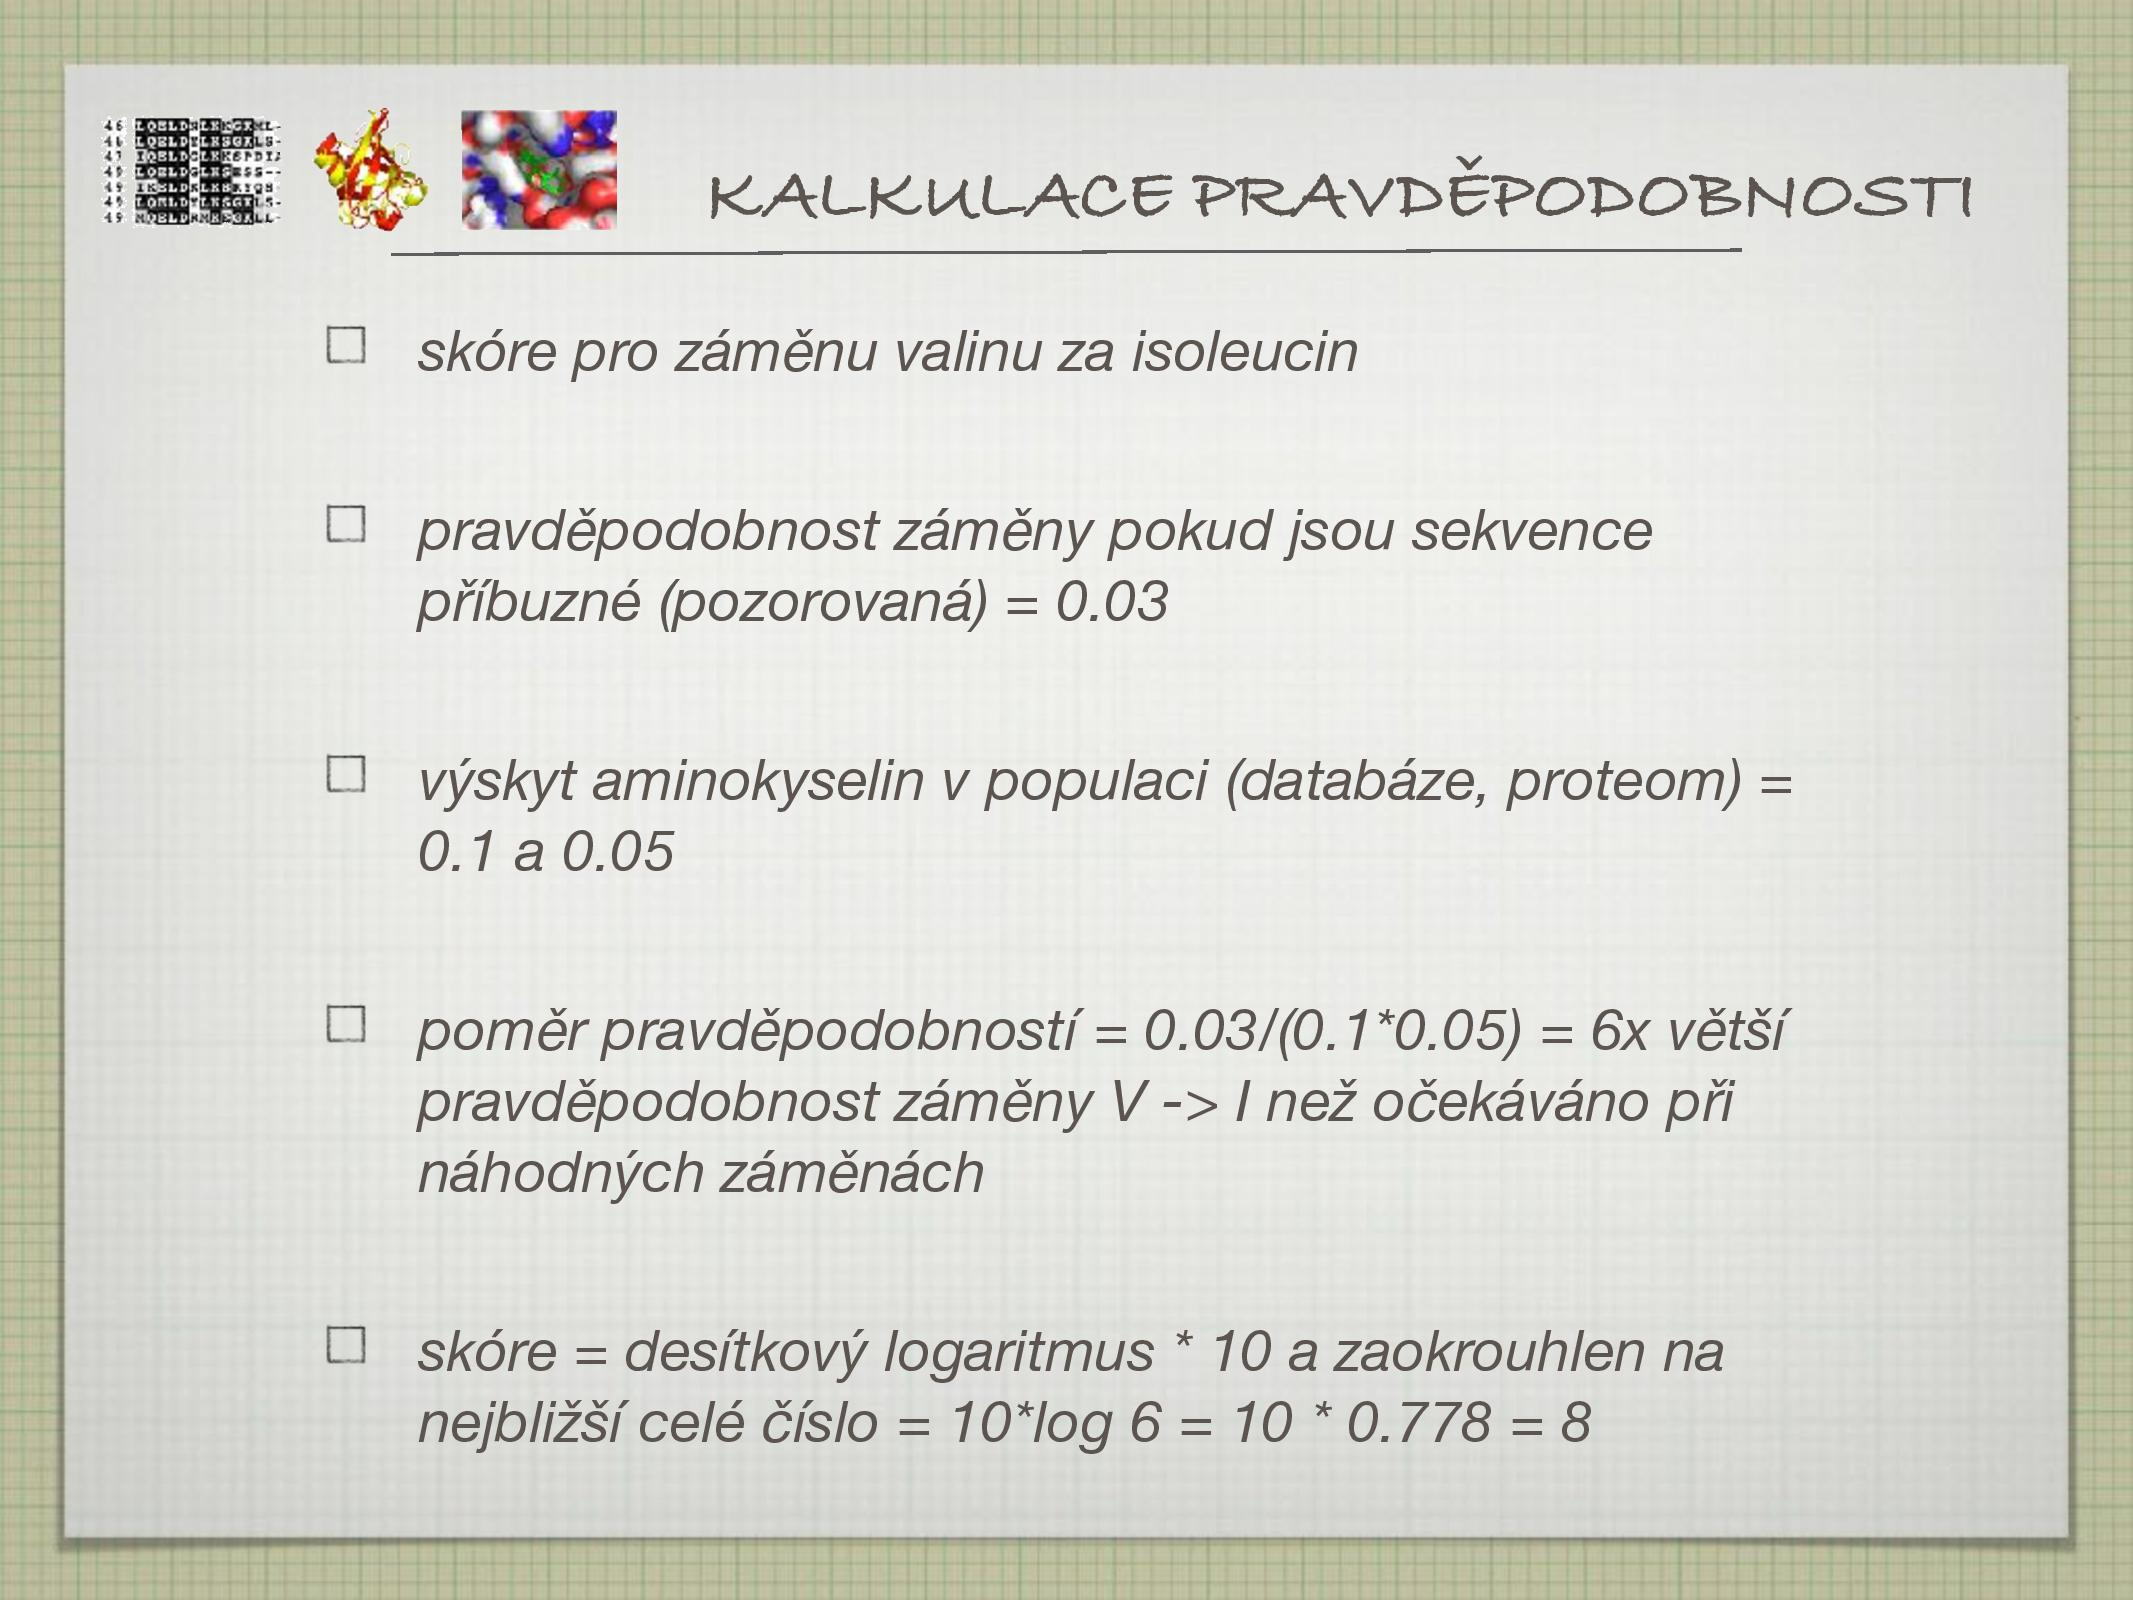
\includegraphics[width=0.85\textwidth]{slides-3/slide-23.jpg}
    \centering
    \label{slides-3-slide-23}
\end{figure}

\paragraph{Tabulka PAM}
\begin{itemize}[nosep]
    \item název z \emph{percent accepted mutations}
    \item autorkou je Margarette Dayhoff (70. léta)
    \item založená na pravděpodobnostních mírách mutace kalkulovaných z globálních alignmentů blízce podobných sekvencí
\[\text{hodnota(X, Y)} = \log \frac{\text{počet pozorovaných záměn X za Y}}{\text{počet očekávaných záměn}}\]
    \item pozitivní je tedy skóre jen u zbytků, u kterých záměna proběhla častěji než by bylo očekáváno při náhodném zaměňování
    \item PAM tabulek je mnoho
\begin{itemize}[nosep]
    \item PAM \(x\) -> \(x\) AK ze 100 bylo nahrazeno
    \item nízké \(x\) se tedy hodí pro evolučně blízké sekvence, vysoké \(x\) pro ty vzdálené
    \item nejoblíbenější PAM 250
\begin{itemize}[nosep]
    \item každá AK byla v průměru zaměněna 2,5 krát
    \item některé AK jsou ale mutovány vícekrát, proto jsou i takové sekvence asi z 20\% složené ještě z původních AK
\end{itemize}

    \item nyní už existují novější tabulky, které jsou generované stejným způsobem, ale z většího množství dat: PET
\end{itemize}

\end{itemize}



\begin{figure}
    \caption{Prezentace č. 3, slide č. 29}
    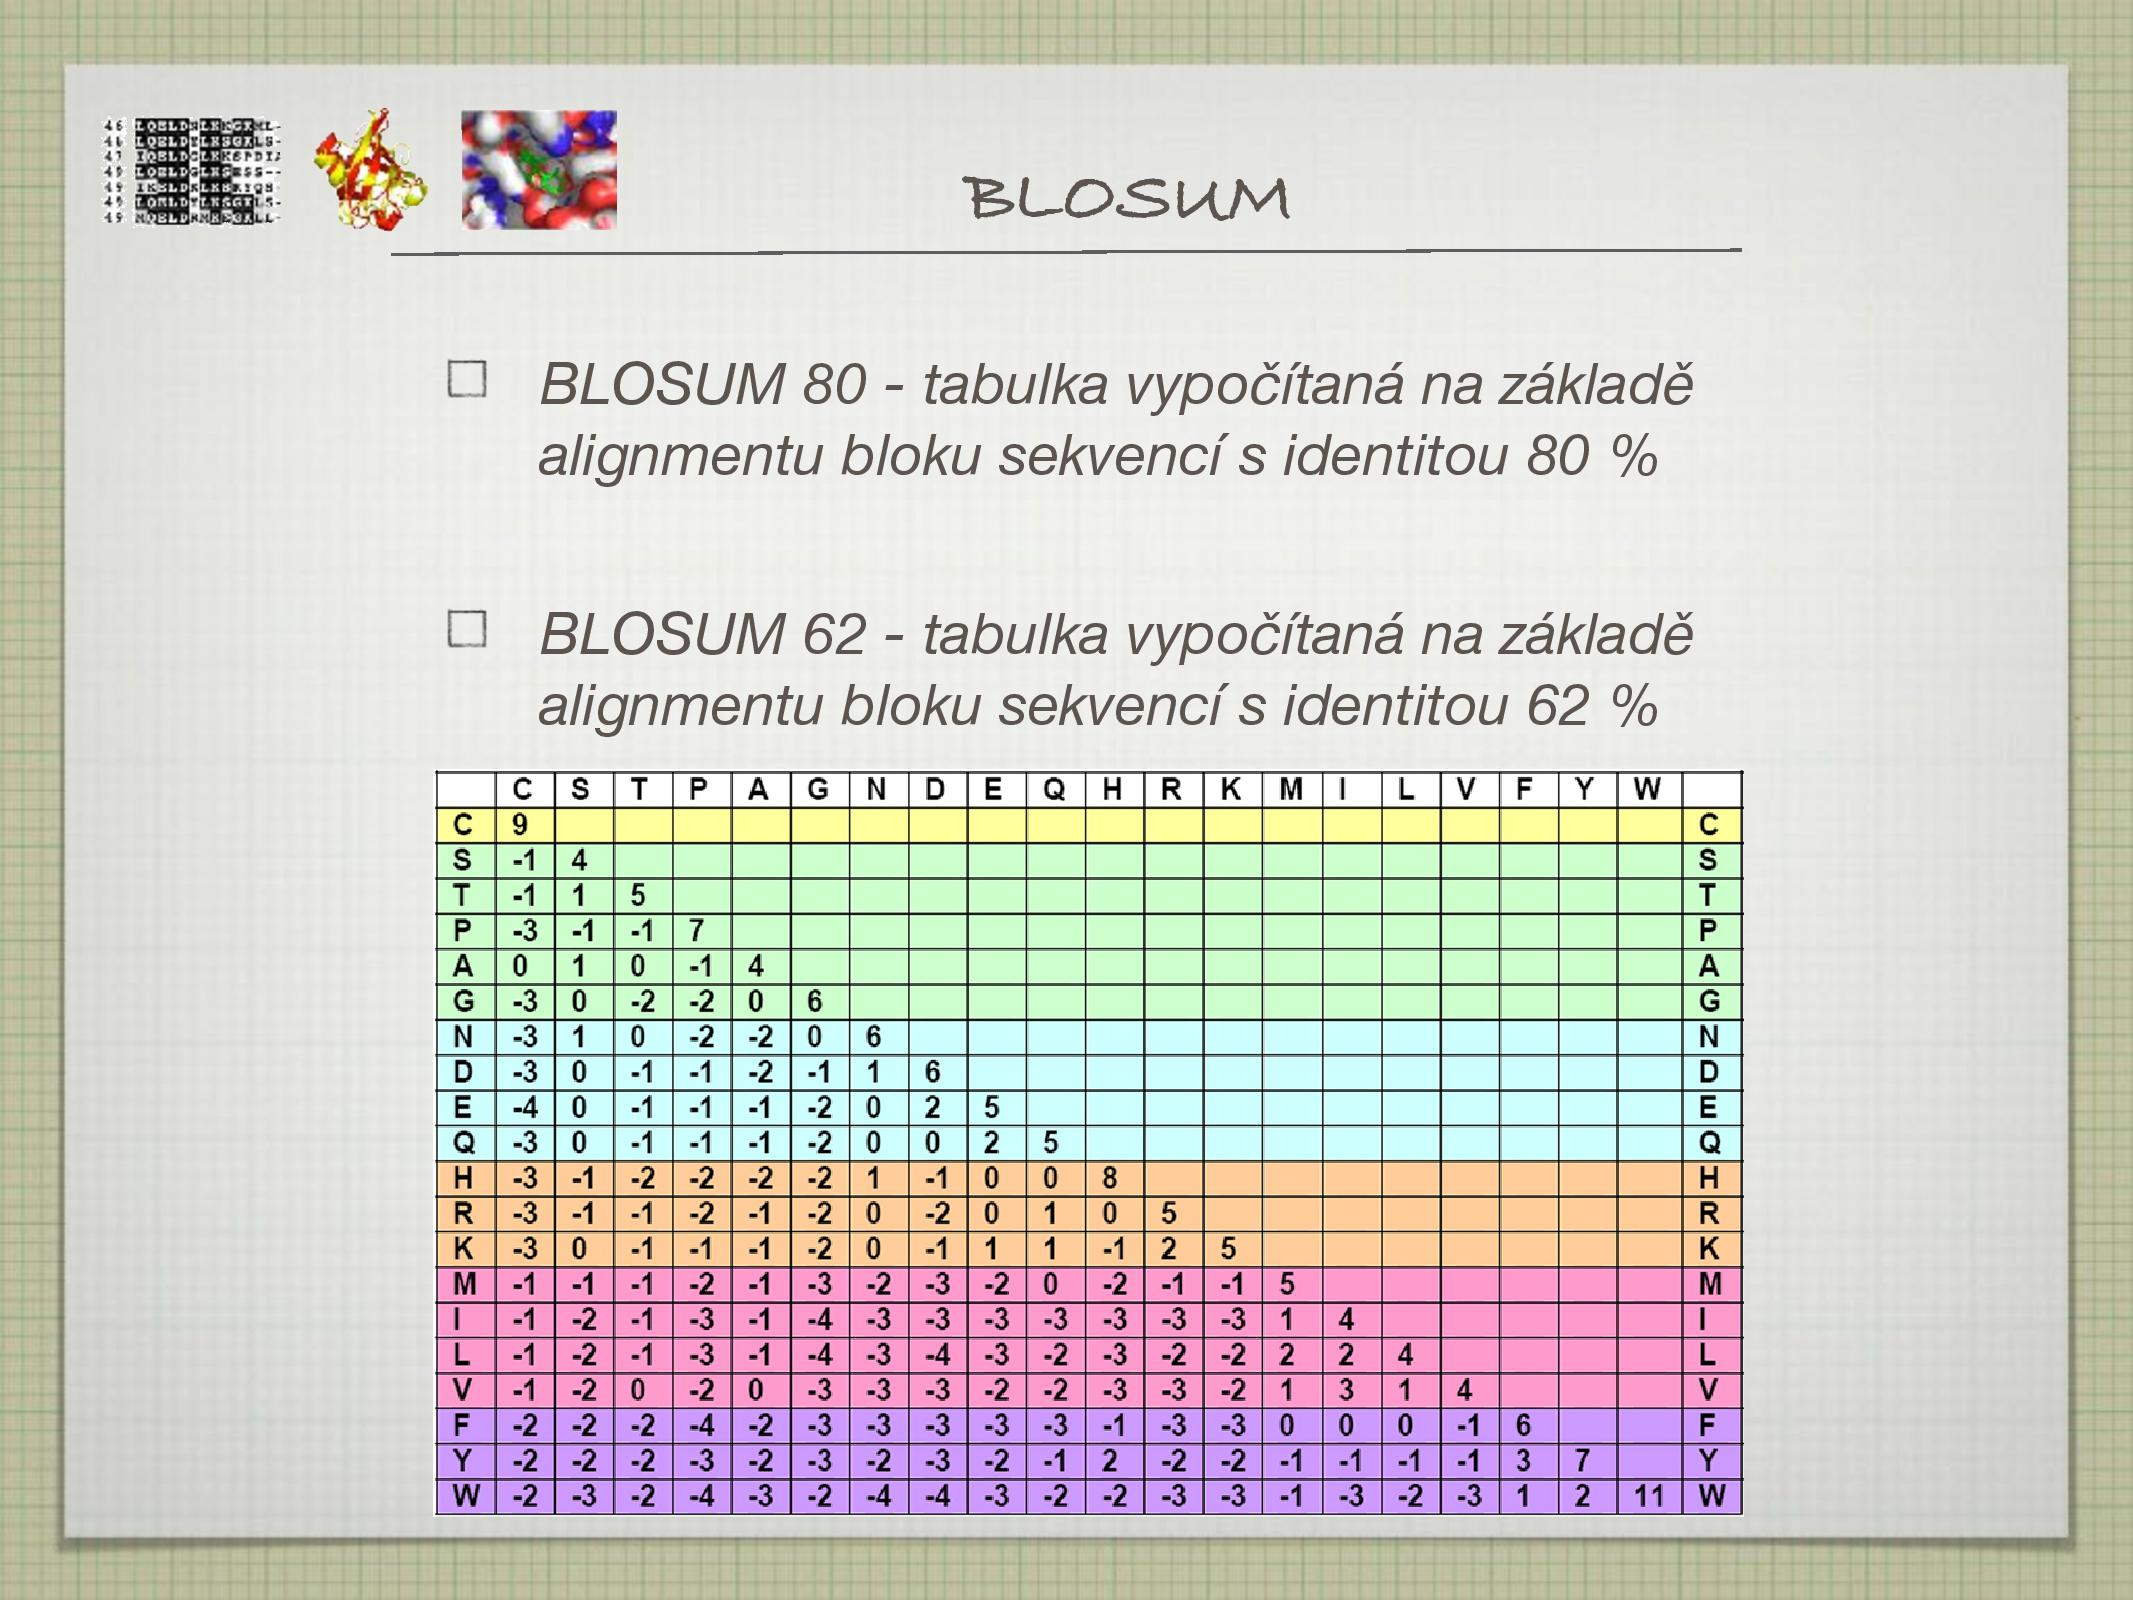
\includegraphics[width=0.85\textwidth]{slides-3/slide-29.jpg}
    \centering
    \label{slides-3-slide-29}
\end{figure}

\paragraph{Tabulka BLOSUM}
\begin{itemize}[nosep]
    \item název z \emph{BLOck SUbstitution Matrix}
    \item autoři Henihoff a Henihoff (90. léta)
    \item založena na experimentálních datech, není extrapolována jako některé PAM tabulky
    \item opět více druhů
\begin{itemize}[nosep]
    \item BLOSUM \(x\): založena na lokálních alignmentech bloků AK s \(\text{SI}=x\) (u homologních proteinů), bez mezer
    \item nejoblíbenější BLOSUM 80 (tedy popsiující proteiny se sekvenční identitou 80\%)
\end{itemize}

\end{itemize}



\paragraph{Další tabulky}
\begin{itemize}[nosep]
    \item STR, SDM
\begin{itemize}[nosep]
    \item informace ze struktur
    \item záměny ve smyčkách jsou pravděpodobnější než v helixech a listech
\end{itemize}

    \item PHAT, SLIM \begin{figure}
    \caption{Prezentace č. 3, slide č. 33}
    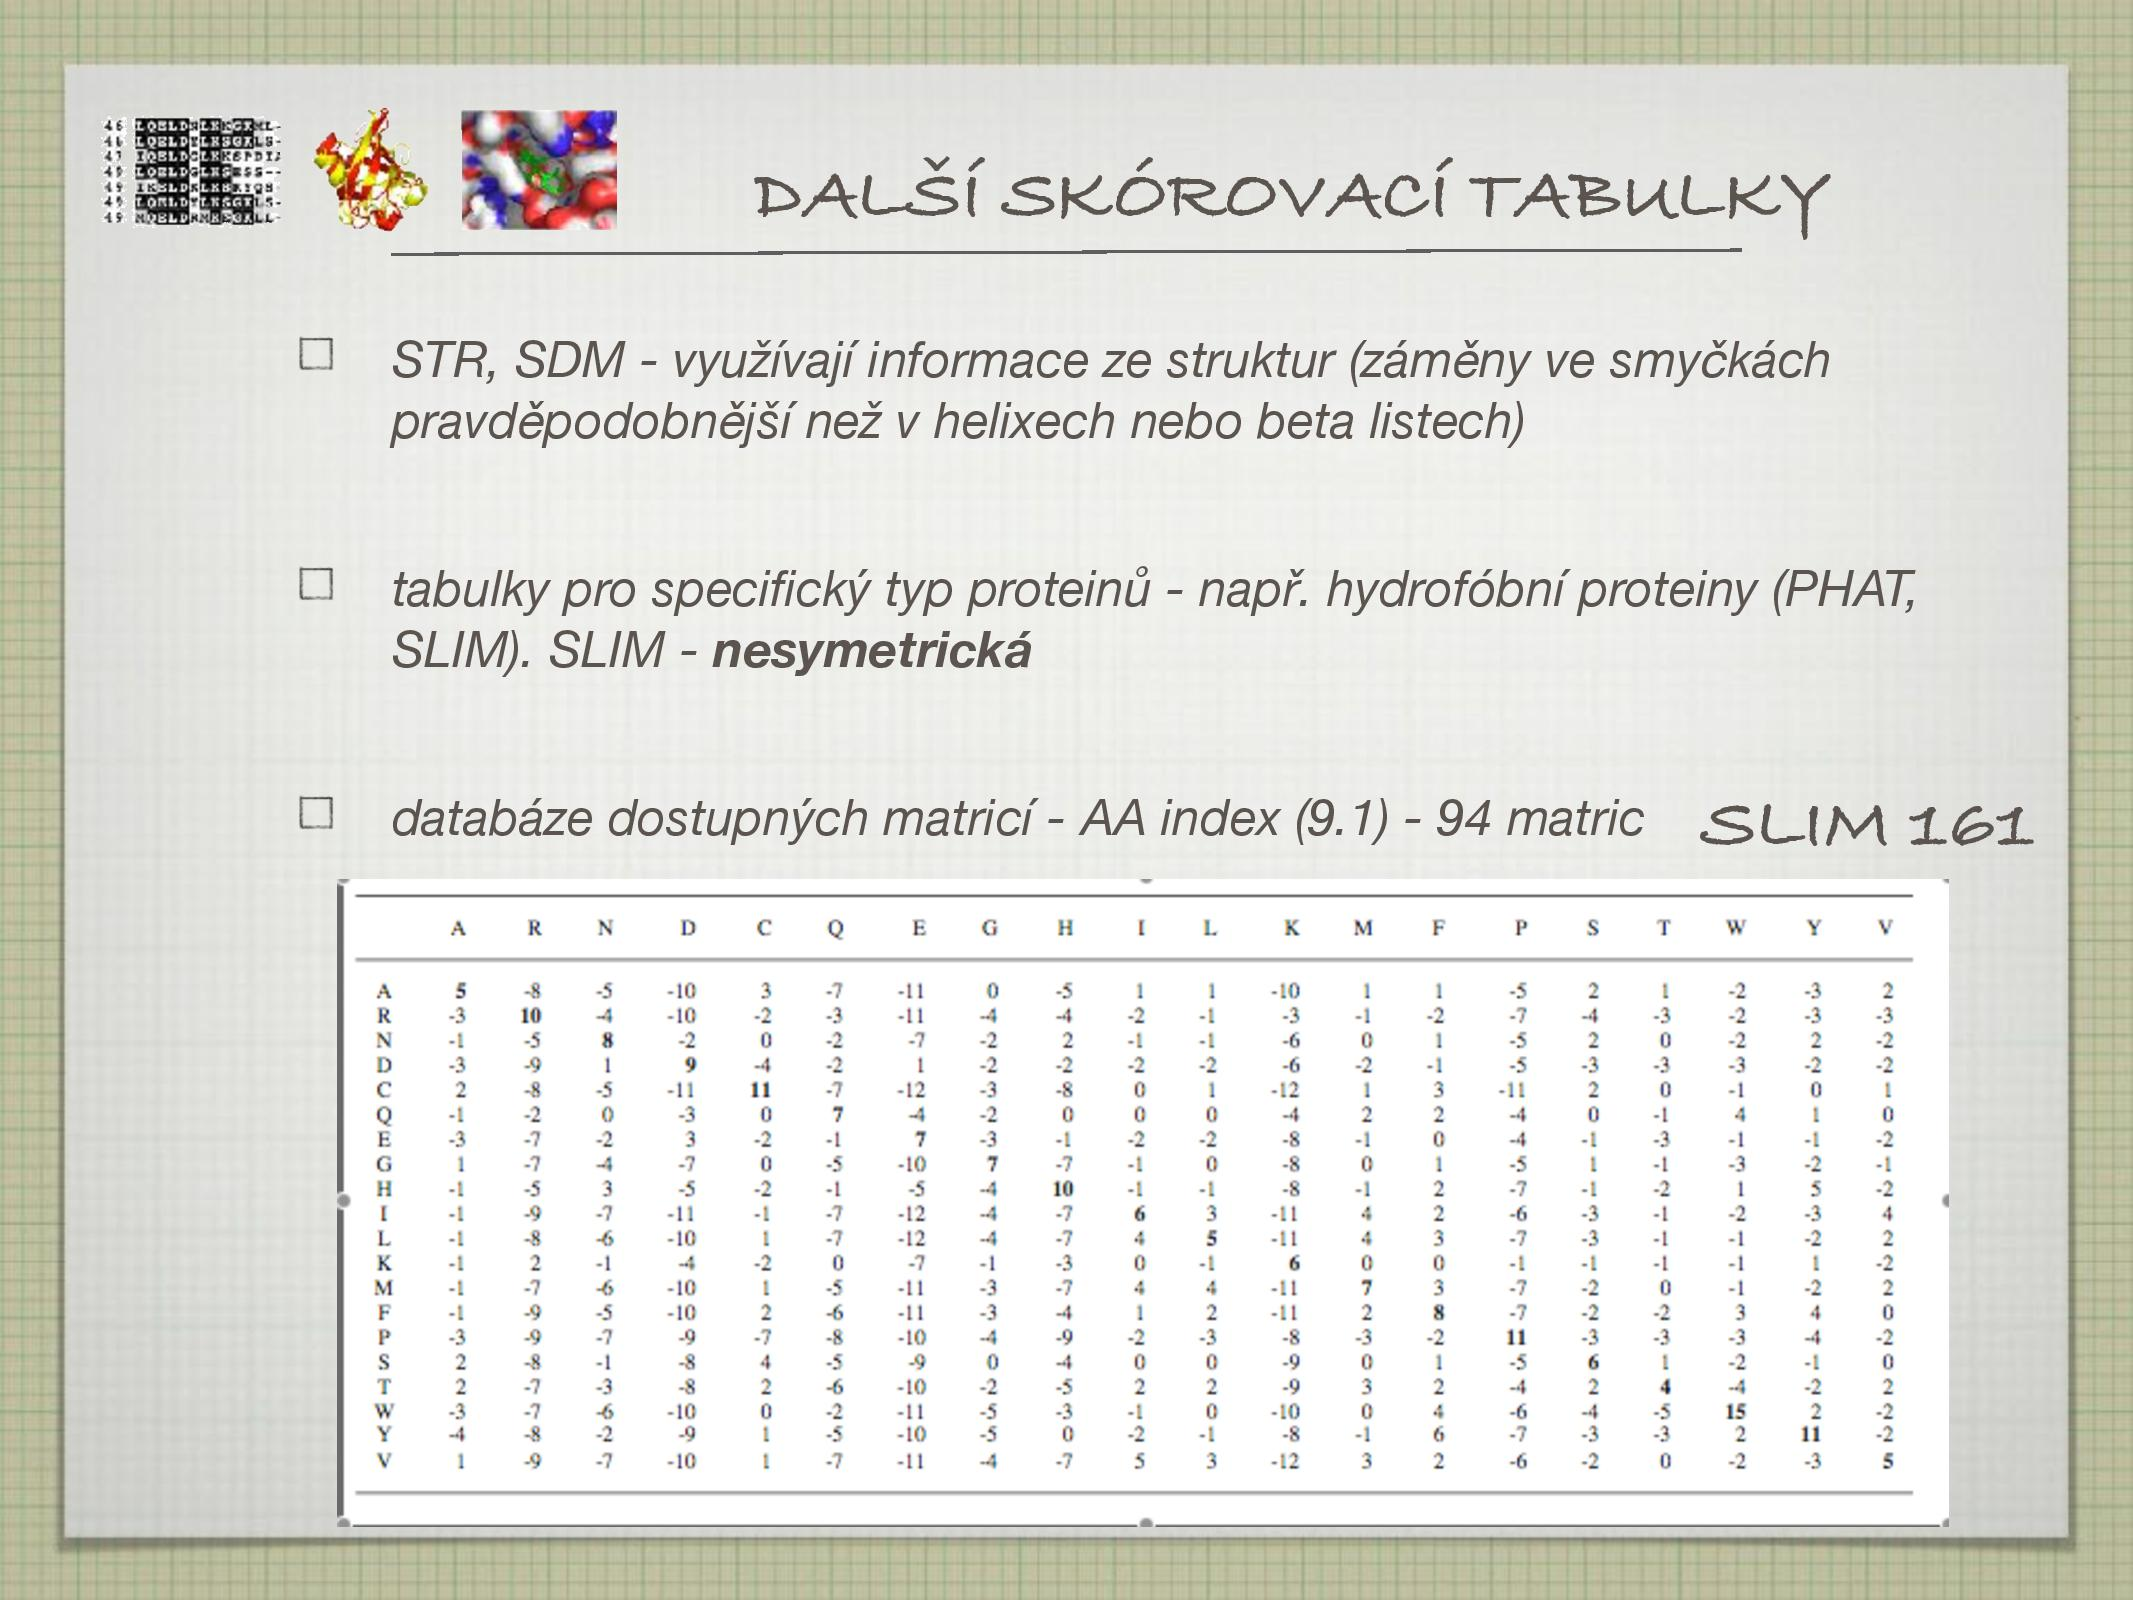
\includegraphics[width=0.85\textwidth]{slides-3/slide-33.jpg}
    \centering
    \label{slides-3-slide-33}
\end{figure}

\begin{itemize}[nosep]
    \item vhodné pro specifický výběr proteinů (například hydrofobní)
    \item SLIM je asymetrická
\end{itemize}

\end{itemize}



\begin{figure}
    \caption{Prezentace č. 3, slide č. 31}
    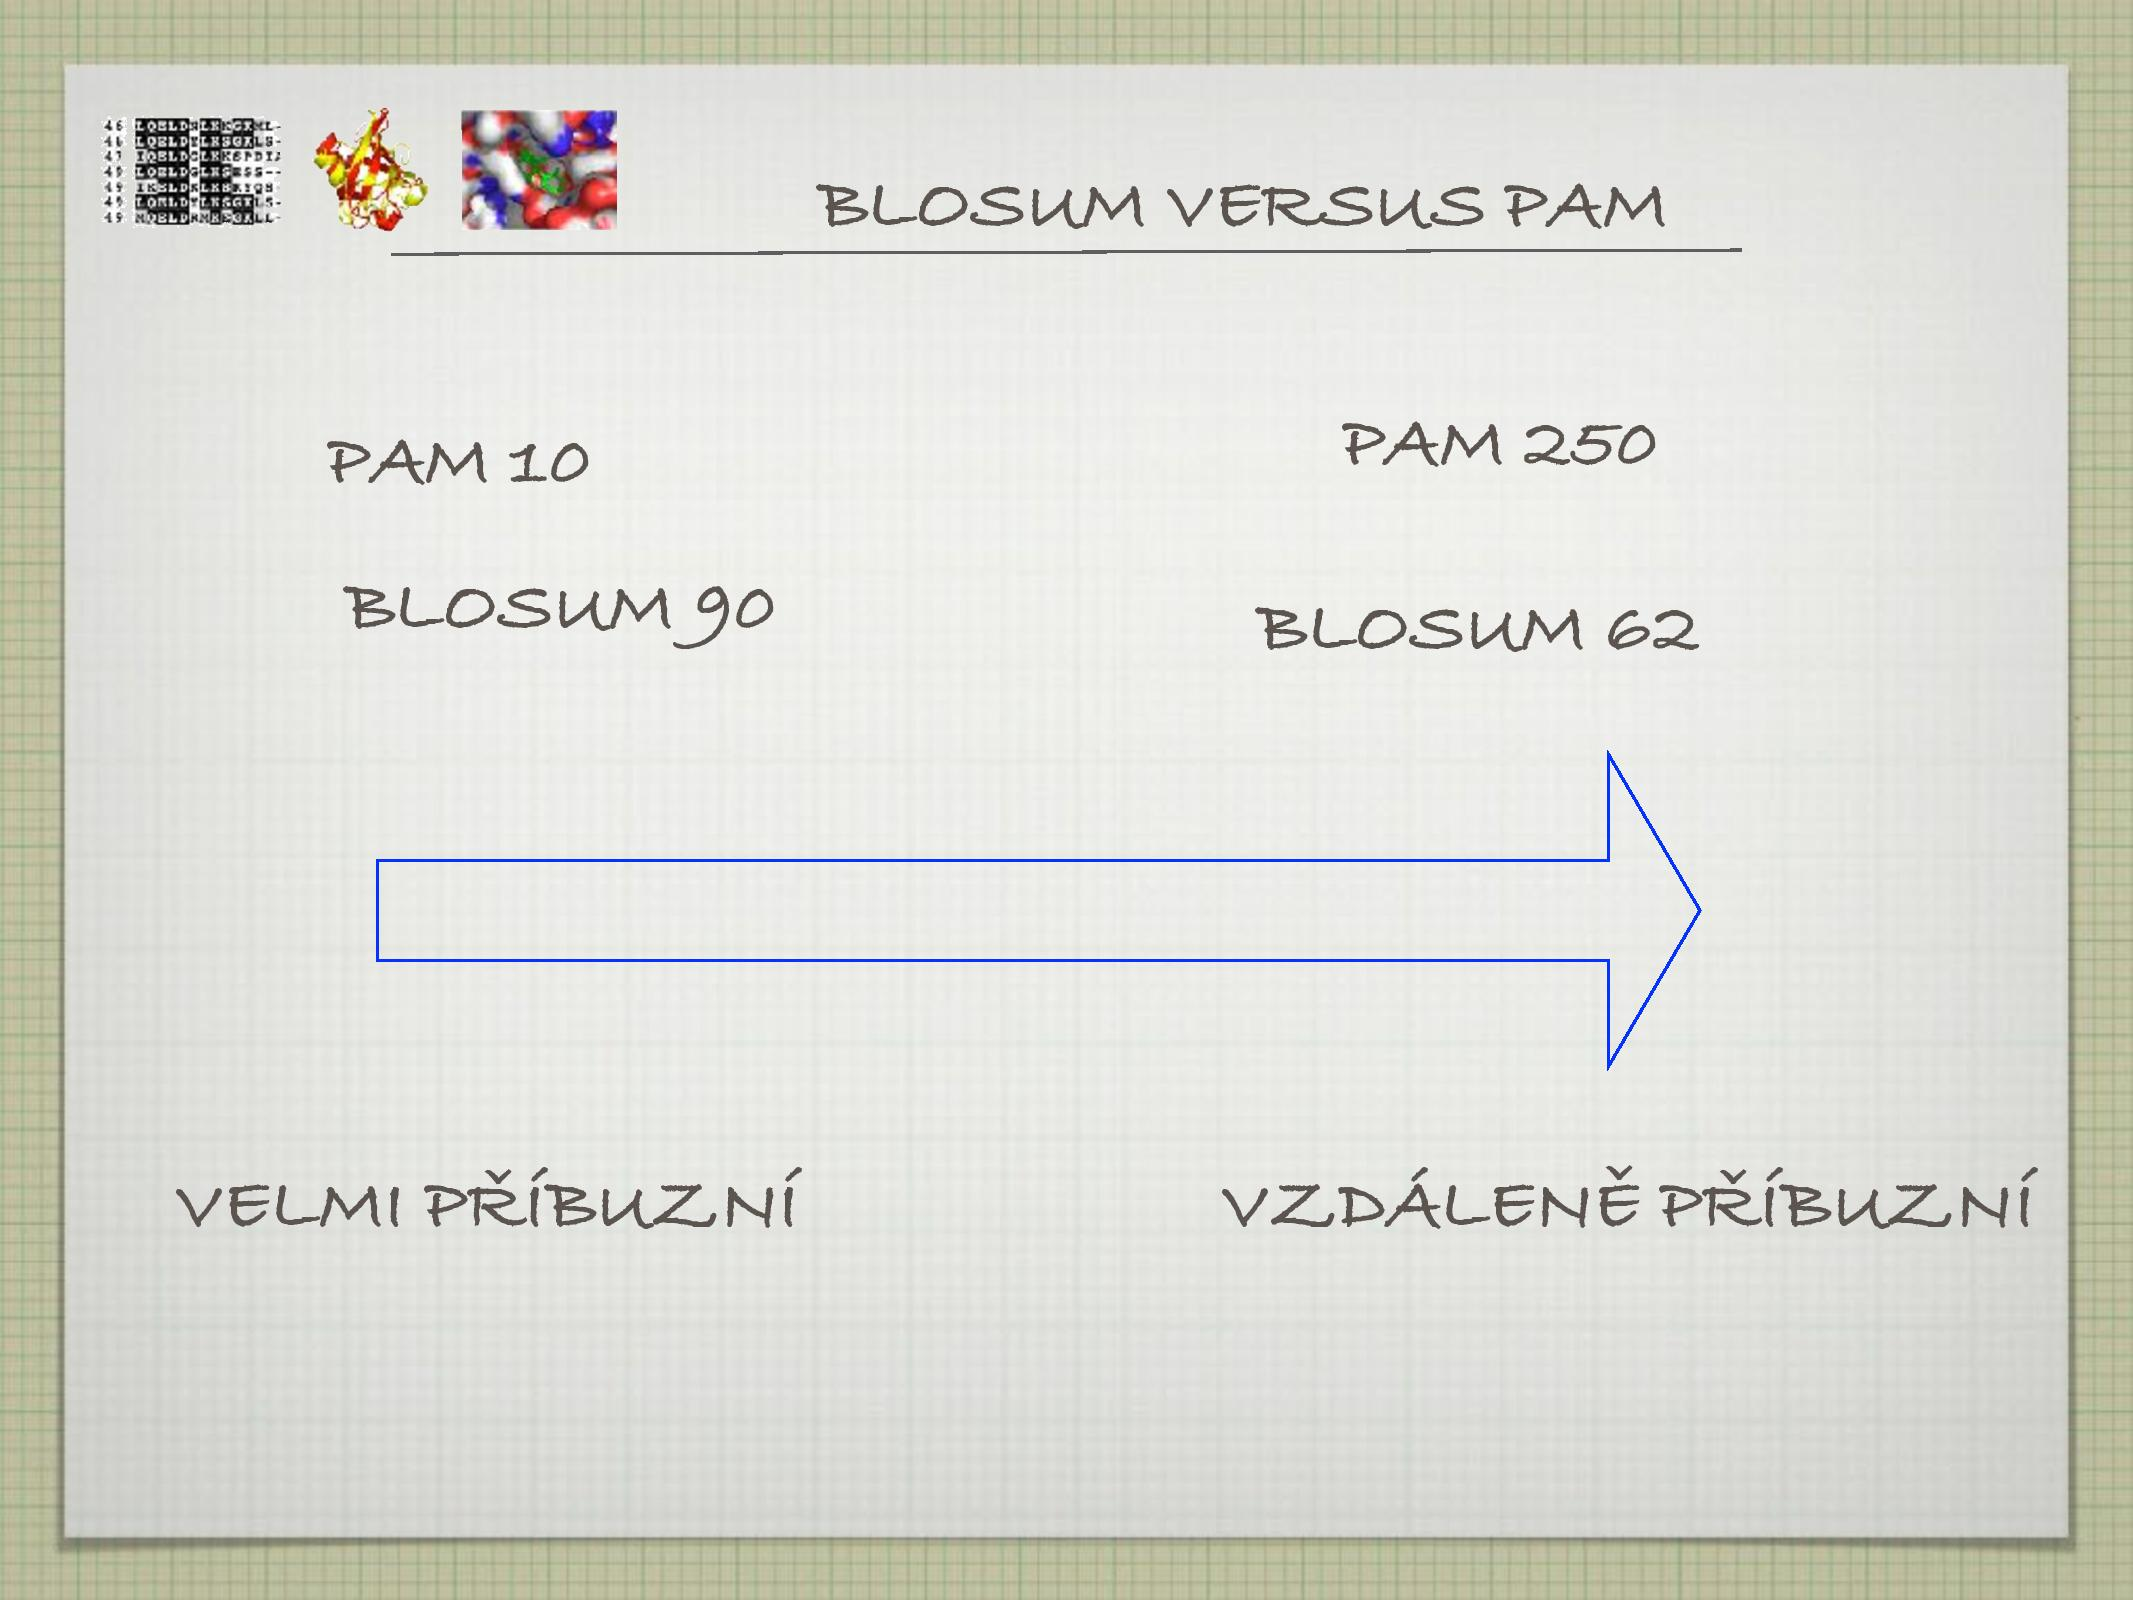
\includegraphics[width=0.85\textwidth]{slides-3/slide-31.jpg}
    \centering
    \label{slides-3-slide-31}
\end{figure}


Výběr tabulky se snažíme přizpůsobit sekvencím, které srovnáváme, abychom získali co nejlepší výsledky; především rozlišujeme evolučně blízké sekvence od těch vzdálených. Krátké sekvence skórujeme podle tabulek pro krátký evoluční čas.

\subsection{Algoritmy} \label{Algoritmy}


\paragraph{Needleman-Wunsch}
\begin{itemize}[nosep]
    \item hledá globální alignment
    \item pracuje na principu dynamického programování
    \item jeden z nejstarších (1970)
    \item zaručuje nalezení optimálního alignmentu (vzhledem k dané GP a skórovací tabulce)
\end{itemize}



\begin{figure}
    \caption{Prezentace č. 3, slide č. 44}
    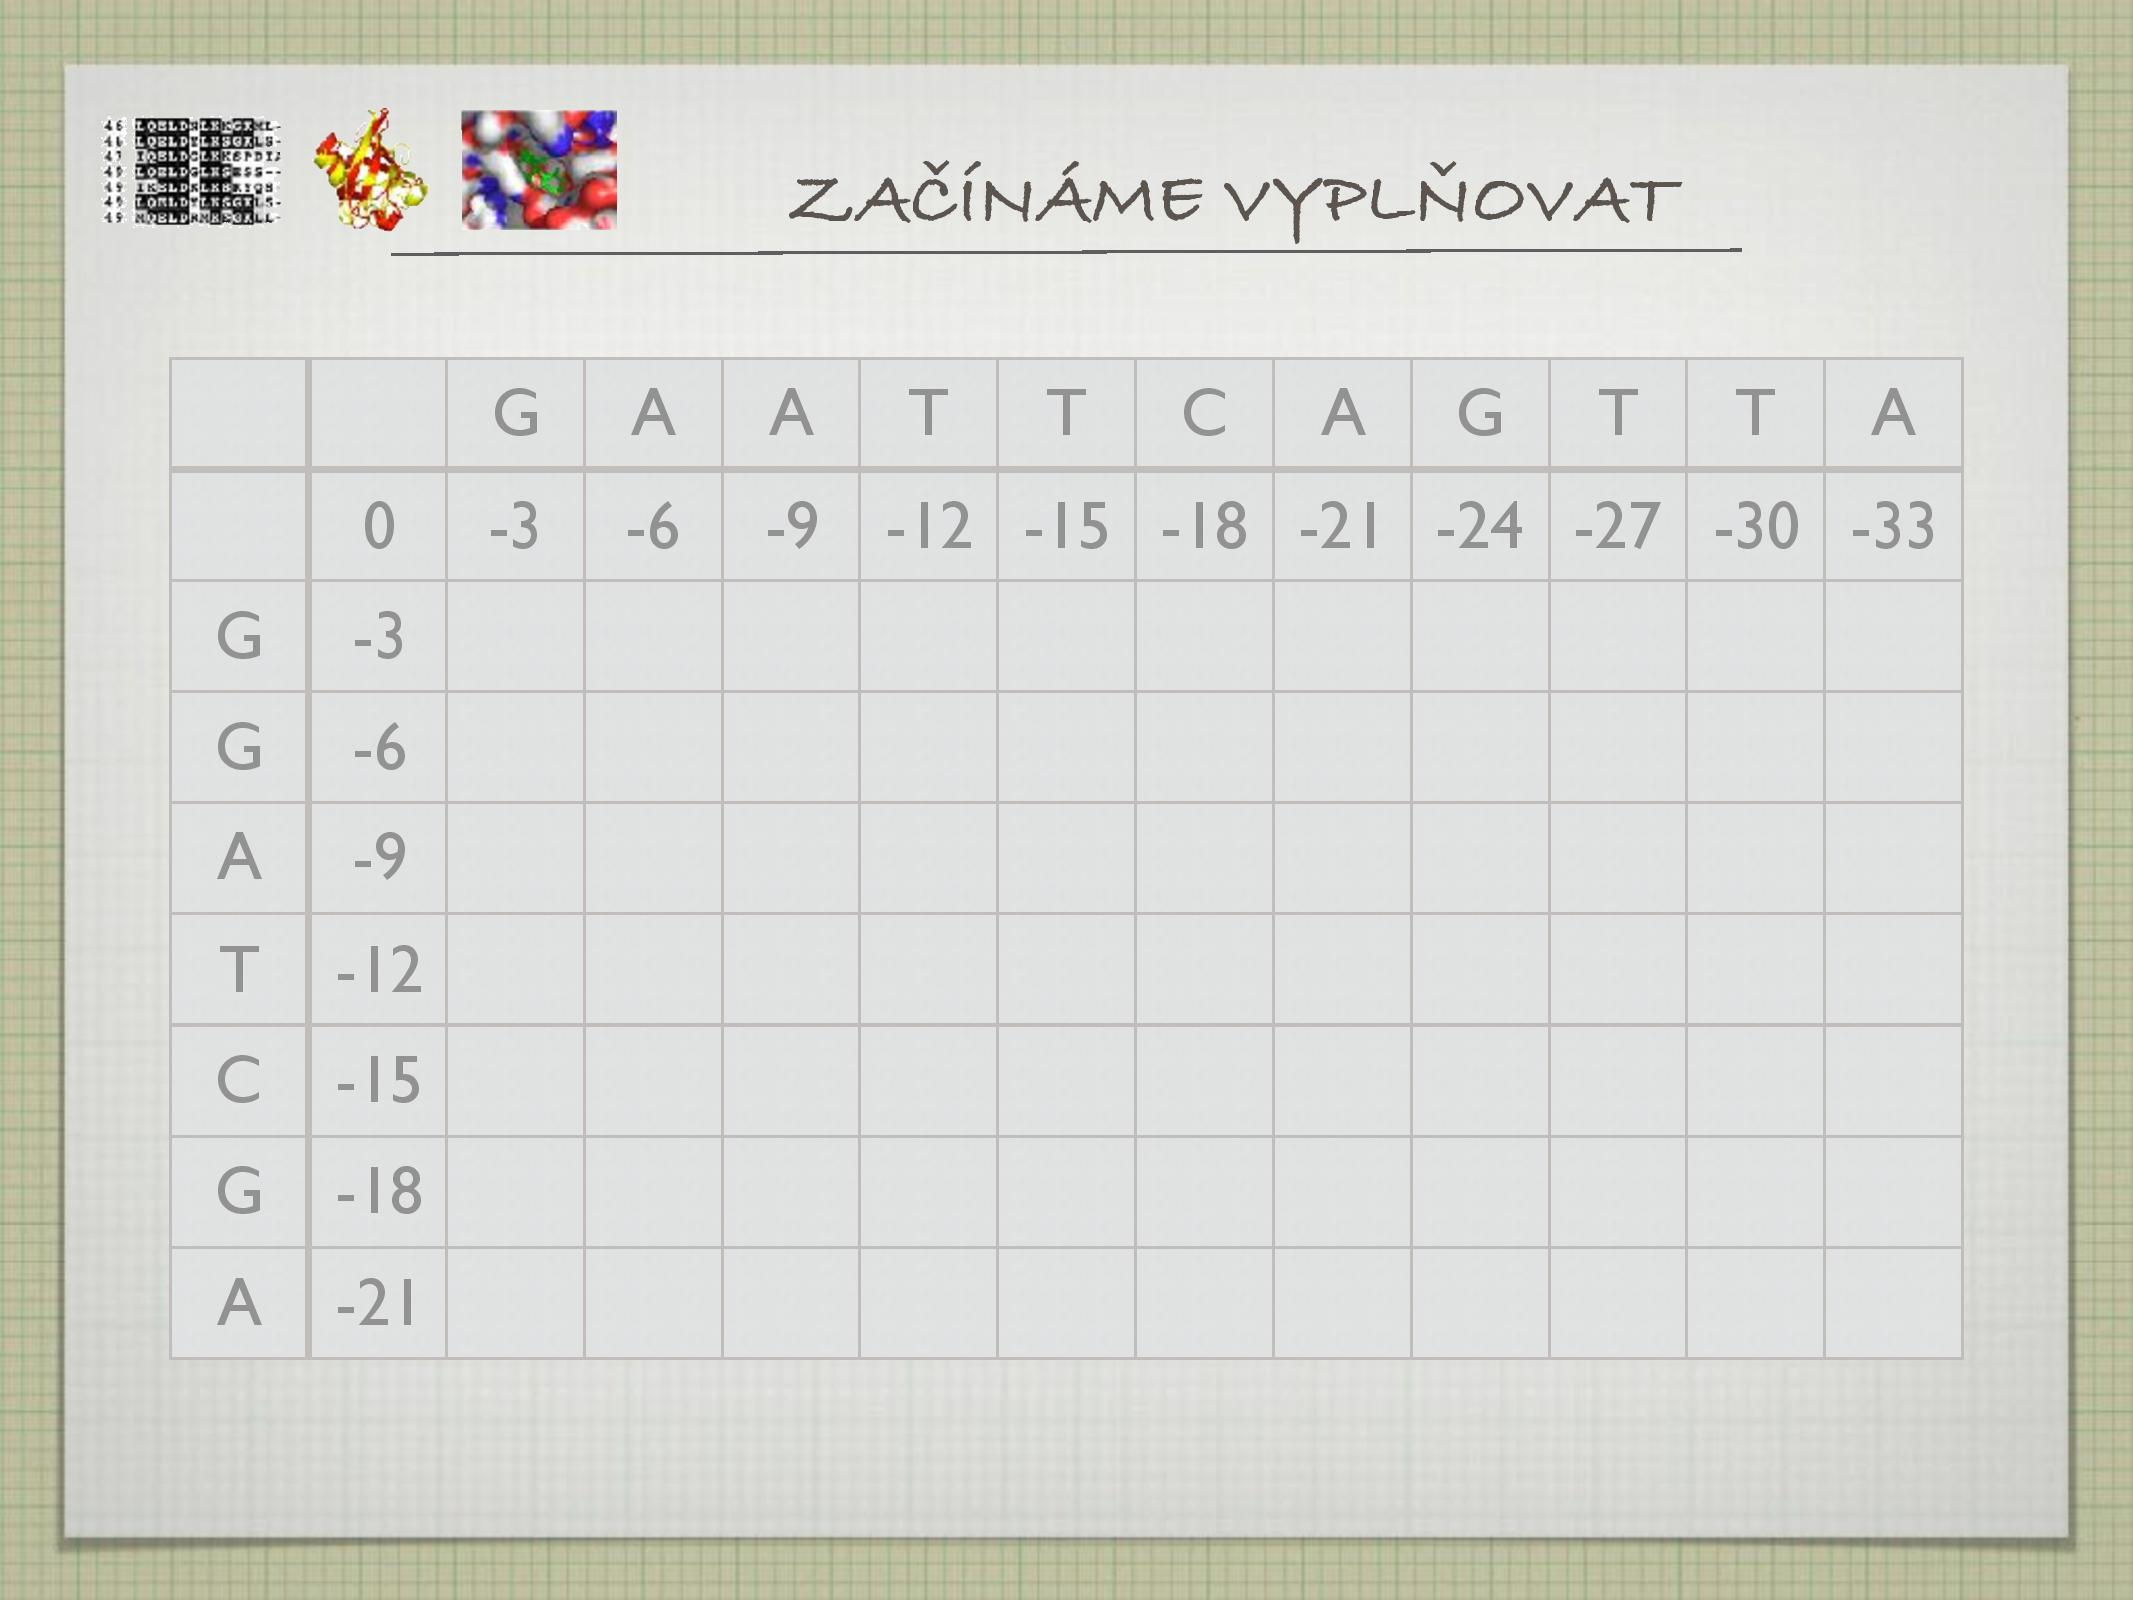
\includegraphics[width=0.85\textwidth]{slides-3/slide-44.jpg}
    \centering
    \label{slides-3-slide-44}
\end{figure}
\begin{figure}
    \caption{Prezentace č. 3, slide č. 45}
    \includegraphics[width=0.85\textwidth]{slides-3/slide-45.jpg}
    \centering
    \label{slides-3-slide-45}
\end{figure}
\begin{figure}
    \caption{Prezentace č. 3, slide č. 49}
    \includegraphics[width=0.85\textwidth]{slides-3/slide-49.jpg}
    \centering
    \label{slides-3-slide-49}
\end{figure}
\begin{figure}
    \caption{Prezentace č. 3, slide č. 51}
    \includegraphics[width=0.85\textwidth]{slides-3/slide-51.jpg}
    \centering
    \label{slides-3-slide-51}
\end{figure}
\begin{figure}
    \caption{Prezentace č. 3, slide č. 54}
    \includegraphics[width=0.85\textwidth]{slides-3/slide-54.jpg}
    \centering
    \label{slides-3-slide-54}
\end{figure}

\paragraph{Průběh NW}
\begin{enumerate}[nosep]
    \item první a druhou sekvenci napíšeme na první sloupec a řádek tabulky (respektive)
    \item pro každou pozici v alignmentu s pomocí scoring matrix počítáme skóre, které bychom dostali:
\begin{itemize}[nosep]
    \item při shodě
    \item při neshodě
    \item při inzerci nebo deleci
\end{itemize}

    \item z těchto možností vždy vybereme tu nejvyšší na napíšeme šipku příslušného směru
    \item postupujeme od konce alignmentu (políčka vpravo dole), a uvažujeme, odkud jsme se na současné políčko dostali
\end{enumerate}



\paragraph{Smith-Waterman}
\begin{itemize}[nosep]
    \item hledá lokální alignment
    \item k hledání podobností mezi proteiny, motivů a domén je vhodnější než NW
    \item funguje podobně jako NW, s několika rozdíly
\begin{itemize}[nosep]
    \item všechna dílčí negativní skóre jsou nahrazena 0
    \item při backtrackingu nezačínáme vpravo dole, ale na políčku s nejvyšším skóre
    \item končíme, jakmile narazíme na 0
\end{itemize}

    \item vzniká alignment pouze dobře konzervovaných úseků
\end{itemize}



Nejznámějším programem na hledání alignmentu je Clustal \(\Omega\) (kdysi Clustal W).


\section{Multiple sequence alignment} \label{Multiple sequence alignment}

\marginline{Přednáška č. 5}

Když srovnáváme více sekvencí najednou, je to sice složitější, ale má to několik velkých výhod:
\begin{enumerate}[nosep]
    \item výsledný alignment je přesnější
    \item data z alignmentu se dají použít pro fylogenetické studie
    \item máme větší šanci nalézt strukturně nebo funkčně významné AK
\begin{itemize}[nosep]
    \item takové AK budou v sekvencích konzervované
\end{itemize}

    \item alignment slouží jako základ pro studie funkce proteinu
\end{enumerate}



\begin{figure}
    \caption{Prezentace č. 4, slide č. 16}
    \includegraphics[width=0.85\textwidth]{slides-4/slide-16.jpg}
    \centering
    \label{slides-4-slide-16}
\end{figure}

\paragraph{Jak dělat MSA}
\begin{itemize}[nosep]
    \item \emph{dynamické programování} už není tak dobrá volba
\begin{itemize}[nosep]
    \item počet rozměrů matice roste lineárně s počtem sekvencí, čili počet nutných srovnání roste exponenciálně
\end{itemize}

    \item používají se \emph{hierarchické progresivní metody}
\begin{itemize}[nosep]
    \item všechny dvojice sekvencí jsou alignovány v rámci PSA
    \item alignmenty jsou hierarchicky seřazeny dle míry podobnosti do fylogenetického stromu (viz níže)
    \item finální MSA je budován v krocích --- nejprve jsou naalignovány dvojice nejpříbuznějších sekvencí, poté jsou alignovány dvojice nejpříbuznějších sekvencí z těchto alignmentů atd.
    \item Clustal \(\Omega\), T-Coffee
\end{itemize}

    \item nevýhody hiearchických metod
\begin{itemize}[nosep]
    \item chyby vytvořené v úvodních alignmentech se dostanou až do finálního výsledku
\begin{itemize}[nosep]
    \item zavedení iterativních metod (optimalizace ohodnocení pomocí \emph{objective function}): Muscle, ProbCons
    \item zavedení učících metod: hidden Markov models, genetické algoritmy, simulated annealing FSA
\end{itemize}

\end{itemize}

\end{itemize}



\begin{figure}
    \caption{Fylogenetický strom (dendrogram)}
    \includegraphics[width=0.85\textwidth]{dendrogram.png}
    \centering
    \label{}
\end{figure}


\paragraph{Programy pro MSA}
\begin{itemize}[nosep]
    \item ProbCons
\begin{itemize}[nosep]
    \item využívá informace z MSA při PSA
    \item mívá nejlepší výsledky
\end{itemize}

    \item FSA (fast statistical alignment)
\begin{itemize}[nosep]
    \item používá machine learning metodu \emph{simulated annealing} na základě PSA
    \item GP i skórovací tabulky jsou odhadovány pro každý set sekvencí individuálně
    \item funguje i pro velice dlouhé sekvence
\end{itemize}

    \item MAFFT
\begin{itemize}[nosep]
    \item metoda pro veliké soubory dat (například fylogenetické analýzy)
    \item homologické oblasti identifikovány pomocí rychlých Fourierových transformací (objem a polarita AK)
    \item výsledný alignment je kombinací progresivních a iterativních metod
\end{itemize}

\end{itemize}



\mybox{Poznámka bokem --- HMM}{HMM je probabilistický model, který se využívá k tvoření obdoby skórovacích tabulek---takových, které jsou alignovaným sekvencím šité na míru. Pro každou pozici ukládá HMM, s jakou pravděpodobností se tam vyskytne jaká AK, s jakou pravděpodobností na daném místě dojde k inzerci a s jakou k deleci. Z těchto údajů dokáže HMM předpovědět sekvence, které do daného modelu zapadají, ale také určit, jak dobře do modelu "sedí" nějaká zadaná sekvence.

Je samozřejmě velice důležité co možná nejlépe určit parametry HMM (ony pravděpodobnosti zmíněné výše). To se většinou dělá \emph{trénováním}, kdy se HMM zadají nějké sekvence a on z nich sám vypočítá potřebné pravdepodobnosti, které si poté uloží. HMM poté může rozhodnout, jak velká šance je, že je nějaká zadaná sekvence příbuzná s těmi, na kterých byl vytrénován.}


\paragraph{Kvalita alignmentu}
\begin{itemize}[nosep]
    \item kvalitu lze hodnotit ze strukturních informací
    \item výsledný MSA je porovnáván s databází strukturních alignmentů \textbf{BALiBase}, HomFam
    \item hodnotící programy
\begin{itemize}[nosep]
    \item APDB, který je součástí T-Coffee (což program na MSA)
    \item QuanTest (2017), za pomoci přesnosti predikce sekundárních struktur
\end{itemize}

    \item umožňuje vybrat nejlepší z alternativních alignmentů
    \item kvalita uvnitř alignmentu
\begin{itemize}[nosep]
    \item není uniformní, MSA programy ale často neoznačují, kterým částem věří a kterým ne
    \item pro účely fylogenetických analýz se často vyřazují oblasti se spoustou mezer
    \item pogramy TrimAl, JalView, UGENE
\end{itemize}

\end{itemize}



\chapter{Hledání v databázích} \label{Hledání v databázích}


Jak roste množství biologických dat, roste i nutnost umět v nich dobře vyhledávat; zpravidla se snažíme najít sekvenci podobnou nějaké jiné, kterou zrovna máme. Je tedy samozřejmé, že \textbf{alignment} je součástí procesu vyhledávání, a to často i lokální alignment (vhledávání na základě podobných domén, motivů).

\begin{description}
\item[true positive (TP)]\hfill \\
To, co jsme hledali a našli.


\item[false positive (TP)]\hfill \\
To, co jsme nehledali a přesto našli.


\item[true negative (TN)]\hfill \\
To, co jsme nehledali a nenašli.


\item[false negative (FN)]\hfill \\
To, co jsme hledali, ale nenašli.

\end{description}


Při vyhledávání je nutno brát ohledy na selektivitu a senzitivitu: obě tyto veličiny ale nelze optimalizovat zároveň.

\begin{description}
\item[senzitivita]\hfill \\
Pravděpodobnost, s jakou budou nalezeny sekvence příbuzné k vyhledáváné sekvenci. Čím nižší je, tím méně skutečných výsledků program najde.
\[\text{senzitivita} = \frac{\text{TP}}{\text{TP} + \text{FN}}\]


\item[selektivita]\hfill \\
Pravděpodobnost, s jakou jsou nalezené sekvence příbuzné s vyhledávanou sekvencí. Čím nižší je, tím více nevýsledků se objevuje v rámci výsledku (=> je těžší najít ve výsledcích zajímavé údaje).
\[\text{selektivita} = \frac{\text{TP}}{\text{TP} + \text{FP}}\]


\item[specifita]\hfill \\
Udává s jakou pravděpodobností nebudou nalezeny sekvence, které nejsou příbuzné s vyhledávanou sekvencí.
\[\text{specifita} = \frac{\text{TN}}{\text{TN} + \text{FP}}\]


\item[negative predictive value (NPV)]\hfill \\
Udává s jakou pravděpodobností budou nenalezené sekvence nepříbuzné s vyhledávanou sekvencí.
\[\text{NPV} = \frac{\text{TN}}{\text{TN} + \text{FN}}\]

\end{description}


\section{Algoritmy} \label{Algoritmy}


\begin{itemize}[nosep]
    \item tradiční algoritmy příliš pomalé, využívají se heuristiky
\begin{itemize}[nosep]
    \item vedou rychle k výsledku, který je blízko tomu optimálnímu
    \item trocha přesnosti obětována pro rychlost
    \item FASTA, BLAST
    \item obě použitelné pro proteiny i DNA
\end{itemize}

    \item někdy se používá i machine learning
\begin{itemize}[nosep]
    \item HMM (hidden Markov models)
    \item profiling methods
\end{itemize}

\end{itemize}



\subsection{FASTA} \label{FASTA}


V 80. létech byl vyvinut algoritmus \textbf{FASTA}, který využívá globální alignment. Funguje následovně:
\begin{enumerate}[nosep]
    \item známé sekvence v databázi jsou rozděleny na krátké úseky o délce \(k\) a uloženy vdo vyhledávací tabulky
\begin{itemize}[nosep]
    \item u proteinů \(k \in \{2, 3\}\)
    \item u DNA \(4 \leq k \leq 6\)
\end{itemize}

    \item na stejně dlouhé úseky je nyní rozdělena i hledaná sekvence
    \item úseky z hledané sekvence jsou porovnány s úseky uloženými ve vyhledávací tabulce, jsou zaznamenány shodné úseky i jejich offsety
\begin{itemize}[nosep]
    \item například úsek AB je v hledané sekvenci na začátku, ale AB ve vyhledávací tabulce začíná až na pátém místě, offset je tedy 5
\end{itemize}

    \item nejlepší matche dvojic úseků jsou rozšířeny a oskórovány příslušnou skórovací tabulkou (bez mezer)
    \item nejlepší takové úseky jsou naalignovány s hledanou sekvencí (tentokrát už s mezerami)
    \item výstupem jsou sekvence z databáze, jejichž úseky mají celkově nejvyšší skóre
\end{enumerate}



Z výše zmíněného i vyplývá, jaká je největší nevýhoda FASTA algoritmu. Může se stát, že FASTA některé příbuzné sekvence nenajde --- konkrétně ty, které s tou hledanou nemají \(k\) identit v řadě. Jsou totiž srovnávány úseky o délce \(k\) a v bodě 3. postupují jen úseky 100\% shodné s nějakým úsekem hledané sekvence.

\subsection{BLAST} \label{BLAST}


V 90. létech následoval algoritmus \textbf{BLAST} (Basic Local Alignment Search Tool), který funguje na bázi lokálního alignmentu.

\begin{figure}
    \caption{Prezentace č. 4, slide č. 44}
    \includegraphics[width=0.85\textwidth]{slides-4/slide-44.jpg}
    \centering
    \label{slides-4-slide-44}
\end{figure}
\begin{figure}
    \caption{Prezentace č. 4, slide č. 46}
    \includegraphics[width=0.85\textwidth]{slides-4/slide-46.jpg}
    \centering
    \label{slides-4-slide-46}
\end{figure}
\begin{figure}
    \caption{Prezentace č. 4, slide č. 47}
    \includegraphics[width=0.85\textwidth]{slides-4/slide-47.jpg}
    \centering
    \label{slides-4-slide-47}
\end{figure}
\begin{figure}
    \caption{Prezentace č. 4, slide č. 48}
    \includegraphics[width=0.85\textwidth]{slides-4/slide-48.jpg}
    \centering
    \label{slides-4-slide-48}
\end{figure}

\paragraph{Funkce BLASTu}
\begin{enumerate}[nosep]
    \item známé sekvence v databázi jsou rozděleny na úseky délky \(k\), tzv. \emph{slova} (words)
\begin{itemize}[nosep]
    \item u proteinů je často \(k = 3\)
\end{itemize}

    \item na stejně dlouhé úseky je nyní rozdělena i hledaná sekvence
    \item slova z hledané sekvence jsou porovnávána se slovy získanými ze sekvencí v databázi a podobnosti jsou oskórovány tabulkou (bez mezer); jsou vybrána taková slova z databáze, která dosáhnou předem nadefinovaného minimálního skóre (threshold)
\begin{itemize}[nosep]
    \item pro proteiny se většinou používá běžná Blosum 62 tabulka
\end{itemize}

    \item vybraná slova jsou rozšířována dokud skóre jejich alignmentu roste, dál postupují opět jen dvojice slov s určitým skóre, tzv. \emph{high scoring pairs} (HSPs)
\begin{itemize}[nosep]
    \item dvojicí slov je myšlen pár [slovo z hledané sekvence + odpovídající slovo z databáze slov známých sekvencí]
\end{itemize}

    \item výstupem jsou HSPs seřazené podle svého skóre, je u nich dostupná i \href{Parametry významnosti alignmentu}{E-value}
\end{enumerate}



Základní rozdíl oproti FASTA tkví v bodě 3. Nejsou vybrána pouze 100\% shodná slova, nýbrž všechna slova, která dosháhnou určitého bodového ohodnocení.

Algoritmus BLAST se vyskytuje v několika verzích, mnohé z nich jsou na internetu, například \href{https://blast.ncbi.nlm.nih.gov/Blast.cgi}{zde}.

\paragraph{Druhy BLASTu}
\begin{itemize}[nosep]
    \item BLASTn: hledá DNA sekvenci v DNA databázi
    \item BLASTp: hledá proteinovou sekvenci v proteinové databázi
    \item BLASTx: hledá DNA sekvenci (6 čtecích rámců) v proteinové databázi
    \item tBLASTn: hledá proteinovou sekvenci v DNA databázi
    \item tBLASTx: překládá DNA v překládané DNA databázi
    \item megablast: zvládne více dotazů (queries) najednou
\end{itemize}



\subsection{Srovnání FASTA a BLAST} \label{Srovnání FASTA a BLAST}


\begin{figure}
    \caption{Prezentace č. 4, slide č. 60}
    \includegraphics[width=0.85\textwidth]{slides-4/slide-60.jpg}
    \centering
    \label{slides-4-slide-60}
\end{figure}

\paragraph{Výhody BLASTu}
\begin{itemize}[nosep]
    \item je rychlejší
    \item lépe pracuje s proteiny
    \item má dobré lokální a krátké globální alignmenty
    \item vytváří HSP (high scoring pairs)
    \item umí najít blízké sourozence (co se evoluce týče)
\end{itemize}



\paragraph{Výhody FASTA}
\begin{itemize}[nosep]
    \item lépe pracuje s DNA
    \item má dobré lokální a krátké globální alignmenty
    \item vytváří Smith-Waterman alignmenty
    \item umí najít vzdálenější sourozence ("sestřenice a bratrance")
\end{itemize}



Existují také SSearch a GSearch, což jsou rigorózní globální/lokální alignmentovací algoritmy. Jejich běh trvá hodiny.

\subsection{Parametry významnosti alignmentu} \label{Parametry významnosti alignmentu}


\begin{description}
\item[Z-score]\hfill \\
Říká nám, jak moc je naše skóre odlišné od toho průměrného. \(\text{ZS} > 15\) je statisticky významné, pro \(5 \leq \text{ZS} \leq 15\) se pravděpodobně jedná o homology a při \(\text{ZS} < 5\) sekvence sice mohou, ale nemusí být homologní.

\paragraph{Postup výpočtu}
\begin{enumerate}[nosep]
    \item uděláme alignment dvou sekvencí a zaznamenáme skóre
    \item jednu sekvenci náhodně přeházíme
    \item znovu uděláme alignment a zaznamenáme skóre
    \item spočítáme průměr a standardní odchylku skóre
\end{enumerate}



\[\text{Z-score} = \frac{\text{průměr skóre}}{\text{standartní odchylka}}\]


\item[P-value]\hfill \\
Existují dvě různé definice, přičemž druhá z nich lépe odpovídá realitě a poskytuje lepší výsledky.
\begin{enumerate}[nosep]
    \item pravděpodobnost, že alignment nepříbuzných sekvencí (FP hit) bude mít stejné nebo vyšší skóre
    \item pravděpodobnost, že bude stejného nebo vyššího skóre dosaženo náhodou
\end{enumerate}



\begin{figure}
    \caption{Prezentace č. 4, slide č. 68}
    \includegraphics[width=0.85\textwidth]{slides-4/slide-68.jpg}
    \centering
    \label{slides-4-slide-68}
\end{figure}
\begin{figure}
    \caption{Prezentace č. 4, slide č. 69}
    \includegraphics[width=0.85\textwidth]{slides-4/slide-69.jpg}
    \centering
    \label{slides-4-slide-69}
\end{figure}

Rozdělení skóre není normální (podle Gaussovy křivky), ale odpovídá EVD křivce (extreme value distribution). Při normálním rozdělení by docházelo k přeceňování významu dosažených skóre.

Pro skóre \(S > x\) platí
\[\text{P-value} = 1 - e^{-e^{-\lambda (x - u)}},\]
kde
\begin{itemize}[nosep]
    \item \(u\) je charakteristická hodnota, \(u = Kmn / \lambda\)
    \item \(m, n\) jsou délky sekvencí
    \item \(K\) je konstanta
    \item \(\lambda\) je "decay factor"
\end{itemize}


\(K\) a \(\lambda\) se dají spočítat ze skórovací tabulky.


\item[E-value]\hfill \\
Pravděpodobnost, že bude v databázi o dané velikosti náhodou dosaženo stejného nebo vyššího skóre.

\[\text{E-value} = \text{P-value} \cdot \text{velikost databáze}\]

\emph{Cutoff} skóre v BLASTu udává, kolik lze v databázi o dané velikosti průměrně čekat FP. Je to vlastně způsob vyvažování selektivity a senzitivity (nižší cutoff zvyšuje selektivitu).

\end{description}


\subsection{Profilové algoritmy} \label{Profilové algoritmy}

\marginline{Přednáška č. 6}

BLAST přistupuje ke všem sekvencím stejně, existují ale i citlivější metody --- \textbf{profilové}.

\begin{figure}
    \caption{Prezentace č. 5, slide č. 5}
    \includegraphics[width=0.85\textwidth]{slides-5/slide-5.jpg}
    \centering
    \label{slides-5-slide-5}
\end{figure}

\paragraph{Profily}
\begin{itemize}[nosep]
    \item skórovací tabulka šitá na míru (pozičně specifická tabulka pro danou proteinovou rodinu)
    \item pro každou pozici v alignmnetu jsou generována specifická skóre (jak pro záměnu AK, tak pro inzerci a deleci)
    \item \[\text{profilové skóre} = 10 \cdot \text{četnost AK na pozici} \cdot \text{hodnota z tabulky}\]
    \item zvyšují citlivost dané metody
\end{itemize}



Zroku 1997 pochází PSI-BLAST (\emph{position specifix iterative BLAST}). Oproti běžnému BLASTu používá \emph{position specific scoring matrix} (PSSM), což je tabulka obsahující specifická skóre pro každou pozici v sekvenci.

\paragraph{PSI-BLAST}
\begin{enumerate}[nosep]
    \item průběh nejprve jako BLAST, z nejlepších výsledných alignmentů je vytvořena PSSM
    \item další kolo BLASTu, pro počítání skóre je ale použita vypočítaná PSSM
\begin{itemize}[nosep]
    \item po konci druhého kola je vytvořena nová PSSM
\end{itemize}

    \item GOTO 2 (dokud nacházíme nové hity)
\end{enumerate}



Z roku 2009 je CS/CSI BLAST, \emph{context-specific iterative BLAST}.

\paragraph{CS/CSI BLAST}
\begin{itemize}[nosep]
    \item kontext vytváří 12 AK v okolí sledované AK
    \item je schopen najít dvakrát více vzdálených homolgů než běžný BLAST při zachování rychlosti a chybovosti
    \item po dvou iteracích CSI BLAST dostaneme stejné výsledky jako po pěti iteracích PSI-BLAST
\end{itemize}



Poslední profilovou metodou jsou HMM, \emph{hidden Markov models}.

\begin{figure}
    \caption{Prezentace č. 5, slide č. 9}
    \includegraphics[width=0.85\textwidth]{slides-5/slide-9.jpg}
    \centering
    \label{slides-5-slide-9}
\end{figure}

\paragraph{HMM}
\begin{itemize}[nosep]
    \item velice citlivá metoda, vytváří statistický model pro definovanou skupinu sekvencí
\begin{itemize}[nosep]
    \item z modelu počítá pravděpodobnosti výskytu dané AK, ostatních AK, inzerce, delece, ale i výskytu mezery a přechodu mezi jednotlivými stavy
\end{itemize}

    \item používána při rozhodování, zda protein spadá do určité skupiny proteinů, typicky pro sekvence s nízkou \%SI
    \item na základě “tréninku” na sekvencích patřících do jedné skupiny (globiny) generuje pravděpodobnost nejen pro jednotlivé záměny a inzerce a delece, ale i pro přechody mezi nimi
    \item dovede do modelu zahrnout i aminokyseliny, které se v tréninkové skupině nevyskytují
\end{itemize}



\chapter{Analýza sekvencí} \label{Analýza sekvencí}


Co dělat, když vyhledávání v databázích nepřineslo nic zajímavého? Jak přesto nějak využít sekvenci, kterou máme?

\paragraph{Co dělat se sekvencí?}
\begin{itemize}[nosep]
    \item „pattern search“ --- hledání domén, motivů
    \item hledání posttranslačních modifikací --- glykosylace, fosforylace, methylace
    \item hledání buněčné lokalizace
    \item určení, zda se nejedná o membránové proteiny
    \item HCA - Hydrofobic Cluster Analysis
    \item hledání procentuální zastoupení AK – kalmodulin
    \item promotorové oblasti --- hledání DNA vazebných míst
    \item predikce struktury
\end{itemize}



Aneb, ano, máme co dělat, i když nám MSA nic moc neprozradil.

\section{Hledání motivů} \label{Hledání motivů}


\paragraph{PROSITE}
\begin{itemize}[nosep]
    \item databáze motivů spojená s databází Swissprot
    \item motivy jsou kontrolovány ručně
    \item umožňuje hledání motivů v sekvenci, hledání sekvencí se specifickým motivem, vytvoření vlastního motivu
\end{itemize}



\begin{description}
\item[profile]\hfill \\
\begin{figure}
    \caption{Prezentace č. 5, slide č. 17}
    \includegraphics[width=0.85\textwidth]{slides-5/slide-17.jpg}
    \centering
    \label{slides-5-slide-17}
\end{figure}

Kvantitativní popis toho, jak vypadá sekvence --- udání vyskytujících se AK a frekvence výskytu. Většinou se jedná o domény.


\item[pattern]\hfill \\
Funguje podobně jako regex --- pattern udává, které AK se (ne)můžou vyskytovat na daném místě, případně kolikrát.

\begin{lstlisting}
[STAIV]-{ERDL}-[LIVMF]-[LIVM]-D-
-[DSTA]-G-[LIVMFC]-X(2,3)-[DNH]\end{lstlisting}

AK jsou označeny jednopísmenným kódem, mezi nimi jsou pomlčky. V hranatách závorkách jsou vyskytující se AK, naopak ve složených jsou nevyskytující se AK. Číslo v závorce udává počet pozic.

Pattern jako jediný dovede jednoznačně přidělit či vyloučit motiv.

\end{description}


\begin{figure}
    \caption{Prezentace č. 5, slide č. 23}
    \includegraphics[width=0.85\textwidth]{slides-5/slide-23.jpg}
    \centering
    \label{slides-5-slide-23}
\end{figure}
\begin{figure}
    \caption{Prezentace č. 5, slide č. 24}
    \includegraphics[width=0.85\textwidth]{slides-5/slide-24.jpg}
    \centering
    \label{slides-5-slide-24}
\end{figure}

\paragraph{Další databáze motivů}
\begin{itemize}[nosep]
    \item BLOCKS: funguje na podobném principu jako BLAST: automaticky generovaná databáze alignmentů konzervovaných úseků
    \item PRINTS: kde je více motivů kombinovaných do fingerprints, které popisují protein
    \item PRODOM: oblíbeno strukturními biology
    \item PFAM: používá HMM, dobře anotovaná, informace o tom, jak dobře proteiny interagují, jestli mají známou strukturu atd.; jde o databázi proteinových rodin a domén
    \item Gene3D: založena na 3D strukturních alignmentech
    \item INTERPRO: shromažďuje informace z více databází, jde o metaserver
\end{itemize}



\section{Další možnosti analýzy sekvencí} \label{Další možnosti analýzy sekvencí}


\paragraph{Druhy posttranslačních modifikací}
\begin{itemize}[nosep]
    \item fosforylace, methylace: součástí signálních kaskád, regulace exprese
    \item \(\ce{N}\)-, \(\ce{O}\)- glykosylace
    \item myristoylace, palmitoylace: uchycení proteinů do membrán
    \item biotynylace: na lysinech
\end{itemize}



\paragraph{Hledání posttranslačních modifikací}
\begin{itemize}[nosep]
    \item predikce probíhá na AutoMotif Serveru, nebo na některé z neuronových sítí: NetPhos, NetOGlyc, NetNGlyc
    \item často ale nalézáme false positives
\end{itemize}



\begin{figure}
    \caption{Prezentace č. 5, slide č. 30}
    \includegraphics[width=0.85\textwidth]{slides-5/slide-30.jpg}
    \centering
    \label{slides-5-slide-30}
\end{figure}

\paragraph{Zjišťování buněčné lokalizace}
\begin{itemize}[nosep]
    \item nástroj určování funkce proteinu a může usnadnit vývoj nových léků
\begin{itemize}[nosep]
    \item sekretované a mebránové proteiny jsou dobře dostupné pro léky
    \item bakteriální povrchové proteiny jsou dobrými kandidáty pro vakcíny
\end{itemize}

    \item proteiny obsahují signály (sekvenční i strukturní), které je návádějí z cytoplazmy do místa jejich určení
\begin{itemize}[nosep]
    \item jaderné proteiny, membránové proteiny, sekretované proteiny, chloroplastové proteiny, proteiny v ER
\end{itemize}

    \item tradičním nástrojem je PSORT
\begin{itemize}[nosep]
    \item dnes updatovaný na WoLF PSORT (80\% přesnost, 14 000 sekvencí)
\end{itemize}

    \item BaCelLo, LOCtree, SherLoc2, SEcretomeP, PredictNLS
\end{itemize}



\begin{figure}
    \caption{Prezentace č. 5, slide č. 31}
    \includegraphics[width=0.85\textwidth]{slides-5/slide-31.jpg}
    \centering
    \label{slides-5-slide-31}
\end{figure}

\paragraph{Určování membránových proteinů}
\begin{itemize}[nosep]
    \item určování pomocí TMHMM (transmembrane helices HMM) nebo Phobius
\begin{itemize}[nosep]
    \item membránové proteiny mají totiž často transmembránové helixy
\end{itemize}

    \item ne příliš početné, ale velice důležité
    \item integrální proteiny musí alespoň jednou projít hydrofóbní membránou
\begin{itemize}[nosep]
    \item musí mít alespoň dvacet hydrofóbních AK
\end{itemize}

\end{itemize}



\paragraph{Určování promotorových oblastí}
\begin{itemize}[nosep]
    \item zajímá nás, zda se před určitým genem vyskytuje motiv, který by byl dobře rozpoznatelný nějakým transkripčním faktorem (TF)
    \item existuje databáze TRANSFAC obsahující DNA sekvence, které na sebe vážou TF
\begin{itemize}[nosep]
    \item databázi můžeme využít při prohledávání promotorových oblastí
\end{itemize}

    \item existují i novější databáze, ale ty jsou placené a velice drahé
\end{itemize}



\paragraph{Další nástroje k analýze sekvencí}
\begin{itemize}[nosep]
    \item porovnání složení z hlediska AK
    \item vazba iontů
    \item řada specializovaných serverů pro specifické skupiny proteinů (například protilátky)
\end{itemize}



\chapter{Databáze} \label{Databáze}


Databáze jsou strukturovaný soubory dat v počítači, které je možné prohledávat a stahovat. Zakládají se z důvodů organizace, zálohování a proto, aby měl k datům kdokoli relativně jednoduchý přístup.

\paragraph{Vlastnosti databáze}
\begin{itemize}[nosep]
    \item četnost aktualizace dat
    \item četnost aktualizace software
    \item redudance dat
    \item anotace dat (přidělení biologického významu sekvencím)
    \item anotace databáze (kdo databízi vytvořil a co bylo jeho cílem, jak se s daty nakládá, jestli existuje kontrola dat)
\end{itemize}



V databázích nejsou uložena jen data o proteinech:
\begin{itemize}[nosep]
    \item databáze DNA
\begin{itemize}[nosep]
    \item GebBank, EMBL, DDJB
    \item data si denně vyměňují, takže mají stený obsah
\end{itemize}

    \item databáze proteinů
\begin{itemize}[nosep]
    \item UniProt (tj. Swissprot + TrEMBL + PIR): lepší než americké databáze
    \item SwissProt, GenPept, PRF
\end{itemize}

    \item genomové databáze (obsahují nukleotidové sekvence a mapování, z genové mapy umíme předpovědět funkci) \begin{figure}
    \caption{Prezentace č. 5, slide č. 52}
    \includegraphics[width=0.85\textwidth]{slides-5/slide-52.jpg}
    \centering
    \label{slides-5-slide-52}
\end{figure}
\begin{figure}
    \caption{Prezentace č. 5, slide č. 53}
    \includegraphics[width=0.85\textwidth]{slides-5/slide-53.jpg}
    \centering
    \label{slides-5-slide-53}
\end{figure}

\begin{itemize}[nosep]
    \item enembl, sanger
\end{itemize}

    \item strukturní databáze (obsahují 3D struktury molekul)
\begin{itemize}[nosep]
    \item primární: RCSB (USA), PDBe (EU), PDBJ (Japonsko)
\begin{itemize}[nosep]
    \item pravidelně si vyměňují data
\end{itemize}

    \item "added-value" databáze: OCA, PDBSum
    \item odvozené databáze, které hodnotí kvalitu dat: EDS, WhatCheck
\end{itemize}

\end{itemize}



\section{Strukturní databáze} \label{Strukturní databáze}


\paragraph{Způsoby získávání dat}
\begin{itemize}[nosep]
    \item rentgenová krystalografie
\begin{itemize}[nosep]
    \item libovolná velikost proteinu nebo komplexu
    \item potřebujeme ale krystal, který je velmi složité vyrobit
    \item vhodná pro statickaé struktury
    \item má velké rozlišení
\end{itemize}

    \item NMR (nuclear magnetic resonance)
\begin{itemize}[nosep]
    \item limitovaná velikostí proteinu (kolem 50 kDa)
    \item potřebujeme čistý vzorek v roztoku
    \item nezískáme tolik detailů jako u krystalografie
    \item vidíme i vzdálenosti vodíkových atomů a torzní úhly, výsledkem je několik struktur => vidíme i dynamiku
\end{itemize}

    \item elektronová mikroskopie
\begin{itemize}[nosep]
    \item má limitované rozlišení
    \item vhodná pro velké komplexy
    \item většinou používána v kombinaci s krystalografii pro dosažení velkého rozlišení
\end{itemize}

\end{itemize}



\mybox{TODO}{Doplnit odkazy na zápisky ze strukturní biologie (až zde budou).}


\subsection{PDB} \label{PDB}


\begin{figure}
    \caption{Prezentace č. 5, slide č. 63}
    \includegraphics[width=0.85\textwidth]{slides-5/slide-63.jpg}
    \centering
    \label{slides-5-slide-63}
\end{figure}
\begin{figure}
    \caption{Prezentace č. 5, slide č. 65}
    \includegraphics[width=0.85\textwidth]{slides-5/slide-65.jpg}
    \centering
    \label{slides-5-slide-65}
\end{figure}


PDB (protein data bank) je strukturní databáze.

\paragraph{Historie PDB}
\begin{itemize}[nosep]
    \item založena 1971 Walterem Hamiltonen v Brookhaven National Laboratory
    \item na začátku 7 struktur, nyní přes 150 000 struktur
    \item v dnešní době ji řídí konsorcium tří institucí
\end{itemize}



Soubory jsou v PDB uloženy ve formátu \inlinecode{.pdb}. Ten má dvě části; první popisuje, o jakou strukturu se jedná, druhá popisuje už samotnou strukturu (rozložení atomů a vazeb v prostoru). Ve sloupcích jsou pak zapsaná různá další data, viz slide. \emph{Temperature factor} určuje plochu, kde se popisovaný atom vyskytuje; buďto důsledkem nepřesnosti našich měření, či jeho dynamikou.

V databázích nejsou uloženy jen struktury samotné, ale i daší doplňující informace, například:
\begin{itemize}[nosep]
    \item popis kvality struktury
    \item seznam strukturních motivů
    \item seznam 3D modelů celých proteinů i s ligandy
\end{itemize}



\paragraph{Problémy PDB databází}
\begin{itemize}[nosep]
    \item databáze nemůže odmítnout žádná data
\begin{itemize}[nosep]
    \item tím pádem může obsahovat --- a také vskutku obsahuje --- mnoho chyb
    \item kontrola přes WhatCheck, ProCheck, nebo kontrolou Ramachandranova diagramu, nebo použití EDS (electron density server)
\end{itemize}

    \item struktury jsou pouze modely, které ne nutně vyhovují experimentálním datům (existují více interpretací těchto dat)
    \item změnit data může jen jejich autor (po smrti autora už nikdo)
\end{itemize}



\paragraph{Problémy .pdb formátu }
\begin{itemize}[nosep]
    \item počet atomů ve struktuře je omezený na 99 999 AK
    \item málo strukturovaný typ souborů, což je nevýhoda při automatické extrakci dat
    \item nekonzistetní pojmenování polí v řádcích
\end{itemize}



Existují ale nov strukturní formáty, jako \inlinecode{mmCIF} nebo \inlinecode{XML}, které jsou pro počítače dobře čitelné.

\chapter{Strukturní alignment} \label{Strukturní alignment}

\marginline{Přednáška č. 7}

Struktura proteinu je lépe konzervovaná, než sekvence --- struktura totiž určuje jeho funkci, jejíž změna je jen zřídkakdy výhodná, naproti tomu i různé sekvence mohou mít podobnou strukturu, a tedy funkci.

\paragraph{Proč se zajímat o stukturu?}
\begin{itemize}[nosep]
    \item můžeme pozorovat změny konformace při vazbě s ligandem
    \item můžeme odhalit evoluční vztahy mezi proteiny
\begin{itemize}[nosep]
    \item můžeme dokonce odhalovat homologie v twilight (a midnight) zone
\end{itemize}

    \item proteiny lze na základě struktury dále třídit, můžeme v nich vyhledávat motivy atd.
    \item můžeme pomocí ní vylepšit MSA \begin{figure}
    \caption{Prezentace č. 6, slide č. 41}
    \includegraphics[width=0.85\textwidth]{slides-6/slide-41.jpg}
    \centering
    \label{slides-6-slide-41}
\end{figure}
\begin{figure}
    \caption{Prezentace č. 6, slide č. 43}
    \includegraphics[width=0.85\textwidth]{slides-6/slide-43.jpg}
    \centering
    \label{slides-6-slide-43}
\end{figure}
\begin{figure}
    \caption{Prezentace č. 6, slide č. 45}
    \includegraphics[width=0.85\textwidth]{slides-6/slide-45.jpg}
    \centering
    \label{slides-6-slide-45}
\end{figure}

\begin{itemize}[nosep]
    \item pozice mezer závisí na (viz \href{Pairwise sequence alignment}{oddíl o PSA})
\end{itemize}

\end{itemize}



Najít strukturní alignment je složité (NP-složité), navíc ani optimální alignment (podle nějaké naší metriky) nemusí odpovídat reálným biologickým poznatkům.

\paragraph{Postup strukturního alignmentu}
\begin{enumerate}[nosep]
    \item najdeme nějaký alignment pomocí heuristických metod
    \item optimalizujeme jej dle předem stanovených kritérií
    \item zhodnottím jeho statistickou významnost
\end{enumerate}



\begin{figure}
    \caption{Prezentace č. 6, slide č. 50}
    \includegraphics[width=0.85\textwidth]{slides-6/slide-50.jpg}
    \centering
    \label{slides-6-slide-50}
\end{figure}
\begin{figure}
    \caption{Prezentace č. 6, slide č. 51}
    \includegraphics[width=0.85\textwidth]{slides-6/slide-51.jpg}
    \centering
    \label{slides-6-slide-51}
\end{figure}

\textbf{ad 1)} Toto lze dělat několika způsoby:
\begin{itemize}[nosep]
    \item srovnáním pravidelných úseků sekundární struktury (SS)
    \item srovnáním tabulek vzájemných vzdáleností (\emph{distance matrices}) návzájem si odpovídajích atomů
    \item rozebráním struktury na jednotlivé motivy, z nichž každému je přiřazeno jeno písmeno, a přepsáním proteinů do této nové abecedy; textové sekvence motivů edáním alignmentu těchto dvou sekvencí
    \item rozebráním struktury na jednotlivé motivy, z nichž každému je přiřazeno jeno písmeno, a přepsáním proteinů do této nové abecedy; textové sekvence motivů jsou poté srovnány běžným PSA (BLAST, Yakusa)
\end{itemize}



\textbf{ad 2)} Optimalizovány většinou bývají superpozice atomů. Superpozice je vzdálenost dvou \(\ce{C\alpha}\) měřená jako RMSD (root mean square distance); hledají se pak takové konformace/rotace, aby se součet všech takových vzáleností minimalizoval.

\[\text{RMSD} = \sqrt{\frac{d^2}{N}},\]

kde \(d\) je (Euklidovská) vzdálenost dvou atomů \(\ce{C\alpha}\) a \(N\) je počet atomů \(\ce{C\alpha}\).

\textbf{ad 3)} RMSD je k hodnocení nevhodné, protože je to globální parametr citlivý na lokální změny a protože koreluje s délkou alignmentu. Existuje ale několik alternativ:

\begin{figure}
    \caption{Prezentace č. 6, slide č. 57}
    \includegraphics[width=0.85\textwidth]{slides-6/slide-57.jpg}
    \centering
    \label{slides-6-slide-57}
\end{figure}

\begin{itemize}[nosep]
    \item SAS: řeší problém korelace hodnoty RMSD s délkou sekvence
  \[\text{SAS} = \frac{\text{RMSD}}{N}\]
    \item Z-score a E-value, viz \href{Parametry významnosti alignmentu}{para­me­try výz­nam­nos­ti align­men­tu}
    \item TM-score: není závislé na délce, je citlivější (od 0=úplně jiné do 1=shodné)
\end{itemize}



\begin{figure}
    \caption{Prezentace č. 6, slide č. 58}
    \includegraphics[width=0.85\textwidth]{slides-6/slide-58.jpg}
    \centering
    \label{slides-6-slide-58}
\end{figure}

\paragraph{Metody (stránky, algoritmy)}
\begin{itemize}[nosep]
    \item vyplatí se použít více metod
    \item CE, DALI, MATRAS, atd. (viz slide)
\end{itemize}



\section{Klasifikace proteinů} \label{Klasifikace proteinů}


Strukturní alignment lze využít k tvorbě systému struktur (většinou podle domén). Takovýchto "opakovaných" struktur je konečné množství, proto se vyplatí je klasifikovat.

\begin{description}
\item[doména]\hfill \\
Někdy je uvažována jako jednotka evoluce. Je globulární, při foldingu nezávislá na zbytku proteinu, má více kontaktů uvnitř sebe než se zbytkem proteinu. Může se vyskytovat i samostatně.

\end{description}


\begin{figure}
    \caption{Prezentace č. 6, slide č. 66}
    \includegraphics[width=0.85\textwidth]{slides-6/slide-66.jpg}
    \centering
    \label{slides-6-slide-66}
\end{figure}

\paragraph{Klasifikační systémy}
\begin{itemize}[nosep]
    \item SCOP (Single Curious and Overworked Person?)
\begin{itemize}[nosep]
    \item spíše historická kuriozita
    \item srovnávání struktur bylo manuální, o klasifikaci rozhodoval člověk na základě svých znalostí a zkušeností
\end{itemize}

    \item CATH (Class Architecture Topology Homology) \begin{figure}
    \caption{Prezentace č. 6, slide č. 62}
    \includegraphics[width=0.85\textwidth]{slides-6/slide-62.jpg}
    \centering
    \label{slides-6-slide-62}
\end{figure}

\begin{itemize}[nosep]
    \item class: jsou struktury proteinu spíše alfa nebo beta
    \item architecture: kolik jakých SS protein obsahuje (sandwich, roll, TIM barrel) \begin{figure}
    \caption{Prezentace č. 6, slide č. 64}
    \includegraphics[width=0.85\textwidth]{slides-6/slide-64.jpg}
    \centering
    \label{slides-6-slide-64}
\end{figure}
\begin{figure}
    \caption{Prezentace č. 6, slide č. 65}
    \includegraphics[width=0.85\textwidth]{slides-6/slide-65.jpg}
    \centering
    \label{slides-6-slide-65}
\end{figure}

    \item topology: jak vypadajíc smyčky propojující jednotlivé SS
    \item homology: jak jsou si struktury sekvenčně podobné
\end{itemize}

\end{itemize}



Jak je ze slidů vidět, skoro třetina známých super-rodin spadá do deseti foldovacích skupin. Konkrétně TIM barrel například ukazuje na struktury, které mohou mít mnoho různých enzymatických funkcí. Není to ale možno říct s jistotou, stejně jako u jiných složitých struktur.

\marginline{Přednáška č. 8}

\section{Predikce struktury} \label{Predikce struktury}


Primární struktura (sekvence) proteinu bývá často určena experimentálně, můžeme se tedy pokusit predikovat vyšší struktury. Tato predikce nebývá příliš přesná, mívá tzv. \emph{confidence level}, který udává, jak moc je odhad pravděpodobný.

Anfinsen ukázal, že se ribonukleáza po denaturaci sama renaturuje tak, že je schopna vykonávat svou původní funkci a z toho usoudil, že veškerá informace potřebná pro zaujetí struktury je obsažena v sekvenci.

Určení struktury ze sekvence je ale výpočetně velice náročné a někdy ani není možné.

\subsection{Intrinsically disordered proteins} \label{Intrinsically disordered proteins}


Proteiny (nebo jejich části), které nemají v nepřítomnosti vazebného partnera nebo ligandu pevnou sekundární a terciární strukturu.

\paragraph{Proč jsou zajímavé?}
\begin{itemize}[nosep]
    \item bývají pro protein (nebo minimálně pro vědce) důležité
    \item přechod z nestruktorované do strukturované formy je často nezbytný pro funkci proteinu
    \item komplikují alignmenty, znemožňují krystalizaci
\begin{itemize}[nosep]
    \item je tedy dobré je před krystalizací oddělit
\end{itemize}

\end{itemize}



V rámci proteinu jdou části bez pevné struktury často alespoň přibližně poznat, protože mají několik specifických vlastností.

\paragraph{Vlastnosti oblastí bez struktury}
\begin{itemize}[nosep]
    \item mají typické složení
\begin{itemize}[nosep]
    \item malé AK
    \item jen málo hydrofobních AK, jinak by se daná část sbalila do SS
    \item často se opakují stejné AK, mají nízkou sekvenční komplexitu
\end{itemize}

    \item nejsou moc dobře konzervované
\end{itemize}



\begin{figure}
    \caption{Prezentace č. 7, slide č. 15}
    \includegraphics[width=0.85\textwidth]{slides-7/slide-15.jpg}
    \centering
    \label{slides-7-slide-15}
\end{figure}

\paragraph{Predikce oblastí bez struktury}
\begin{itemize}[nosep]
    \item machine learning, meta servery (spojující několik metod dohromady)
    \item predikuje se sekundární struktura, AK složení, dostupnost AK pro rozpuštědlo, hot loops atd.
    \item typická přesnost předpovědí je mezi 60\% a 70\%
    \item Disembl, FoldIndex, DisoPred, SEG, SPOT-dis, AUCpreD \begin{figure}
    \caption{Prezentace č. 7, slide č. 16}
    \includegraphics[width=0.85\textwidth]{slides-7/slide-16.jpg}
    \centering
    \label{slides-7-slide-16}
\end{figure}
\begin{figure}
    \caption{Prezentace č. 7, slide č. 17}
    \includegraphics[width=0.85\textwidth]{slides-7/slide-17.jpg}
    \centering
    \label{slides-7-slide-17}
\end{figure}
\begin{figure}
    \caption{Prezentace č. 7, slide č. 18}
    \includegraphics[width=0.85\textwidth]{slides-7/slide-18.jpg}
    \centering
    \label{slides-7-slide-18}
\end{figure}

\begin{itemize}[nosep]
    \item vyplatí se používat kombinaci těchto programů
\end{itemize}

\end{itemize}



\subsection{Predikce sekundární struktury} \label{Predikce sekundární struktury}


\begin{figure}
    \caption{Prezentace č. 7, slide č. 20}
    \includegraphics[width=0.85\textwidth]{slides-7/slide-20.jpg}
    \centering
    \label{slides-7-slide-20}
\end{figure}

Často chceme určit, který druh SS se v proteinu vyskytuje nejčastěji, případně na kterém místě je jaká SS, abychom podle toho mohli vylepšit alignment, či abychom dané informace využili při stavění kompletního 3D modelu proteinu. Druhy SS většinou rozlišujeme pouze tři: helix, list a "zbytek".

\paragraph{Metody dříve}
\begin{itemize}[nosep]
    \item predikce založená na jedné sekvenci
    \item založeno na preferencích jednotlivých aminokyselin být v určité SS, které byly experimentálně zjištěny a statisticky zpracovány
\begin{itemize}[nosep]
    \item struktur, ze kterých jsme tado data získávali, bylo sedm
\end{itemize}

    \item pouze semiautomatické
    \item přesnost predikce kolem 60 \%
    \item Chou-Fasman, GOR
\end{itemize}



\paragraph{Metody dnes}
\begin{itemize}[nosep]
    \item známe více sekvencí a jejich srtuktur, máme tedy více dat
    \item nové "učící se" algoritmy, jako HMM a neuronové sítě
\begin{itemize}[nosep]
    \item často využití MSA, které napomáhá správné predikci SS
\end{itemize}

    \item přesnost predikce 75\%--80\% (Q3 skóre, neboli predikce tří různých stavů), navíc dostaneme i odhad významnosti predikce pro každou aminokyselinu
    \item JPred, PsiPred, APSSP2
    \item metody jsou benchmarkovány, například benchmarkem EVA
\end{itemize}



\begin{description}
\item[SS propensity]\hfill \\
Udává, v jaké SS se daná AK nejčastěji vyskytuje; to zjistíme z experimentálně naměřených dat.

\[\text{P}[X \text{ je helixový typ}] = \frac{\text{frekvence } X \text{ v helixu}}{\text{frekvence } X}\]

\end{description}


\begin{figure}
    \caption{Prezentace č. 7, slide č. 25}
    \includegraphics[width=0.85\textwidth]{slides-7/slide-25.jpg}
    \centering
    \label{slides-7-slide-25}
\end{figure}

\paragraph{Průkopníci}
\begin{itemize}[nosep]
    \item Chou-Fasman (1974,1978) - původně na 15 strukturách
    \item klasifikuje AK dle statistik jako silné/slabé makers nebo breakers helixu, listu
\begin{itemize}[nosep]
    \item skóre 1/0/-1 (breakers, ani-ani, makers)
\end{itemize}

    \item postup (dva kroky) \begin{figure}
    \caption{Prezentace č. 7, slide č. 26}
    \includegraphics[width=0.85\textwidth]{slides-7/slide-26.jpg}
    \centering
    \label{slides-7-slide-26}
\end{figure}
\begin{figure}
    \caption{Prezentace č. 7, slide č. 28}
    \includegraphics[width=0.85\textwidth]{slides-7/slide-28.jpg}
    \centering
    \label{slides-7-slide-28}
\end{figure}
\begin{figure}
    \caption{Prezentace č. 7, slide č. 29}
    \includegraphics[width=0.85\textwidth]{slides-7/slide-29.jpg}
    \centering
    \label{slides-7-slide-29}
\end{figure}

\begin{enumerate}[nosep]
    \item počátek (tzv. \emph{nukleace})
\begin{itemize}[nosep]
    \item helix, když má okno o velikosti šest skóre alespoň 4
    \item list, když má okno o velikosti pět skóre aspoň 3
\end{itemize}

    \item růst
\begin{itemize}[nosep]
    \item postupuj oběma směry od počátku tak dlouho dokud je v okně o velikosti čtyři skóre alespoň +1
\end{itemize}

    \item má omezenou přesnost, kolem 60\%
    \item částečně způsobená malým datasetem, ze kterého byly vypočítány parametry
    \item SS je určena i jinými věcmi než jen propensitami AK
    \item existují "chameleón" sekvence, ve kterých je na stejné místo predikován list i helix
\end{enumerate}

\end{itemize}



Trochu lepší výsledky než Chou-Fasman má metoda GOR, která scie také počítá propensities pro všech 20 AK na určité pozici, ale závisí u ní i na 16 okolních AK. Výsledná tabulka s čísly je tedy \(20 \times 17\), místo \(20 \times 1\).

\paragraph{Moderní metody}
\begin{itemize}[nosep]
    \item například PHD, která má úspěšnost přes 70\%
\begin{itemize}[nosep]
    \item používá neurální sítě na dvou stupních, MSA
    \item vychází z databáze nepříbuzných proteinů
\end{itemize}

\end{itemize}



\mybox{Vsuvka}{Arteficiální neurální sítě (ANN) jsou adaptivní systémy založené na biologickém modelu nervové soustavy. Dají se trénovat: máme určitý test dataset, na kterém daná ANN optimalizuje své parametry.

Kromě ANN se používají i metody konsenzu: kombinace několika různých metod pro dosažení optimálního výsledku. Například JPRED a NPS. \begin{figure}
    \caption{Prezentace č. 7, slide č. 37}
    \includegraphics[width=0.85\textwidth]{slides-7/slide-37.jpg}
    \centering
    \label{slides-7-slide-37}
\end{figure}
}


\subsection{Predikce membránových proteinů} \label{Predikce membránových proteinů}


\begin{figure}
    \caption{Prezentace č. 7, slide č. 41}
    \includegraphics[width=0.85\textwidth]{slides-7/slide-41.jpg}
    \centering
    \label{slides-7-slide-41}
\end{figure}

\paragraph{Charakteristiké vlastnosti MP}
\begin{itemize}[nosep]
    \item transmembránové helixy mají typickou délku 20--30 AK
    \item AK jsou hydrofobní, aby mohly protnout membránu
\begin{itemize}[nosep]
    \item na konci bývají Trp a Tyr (procházejí kolem polárních hlav lipidů)
    \item na vnitřní straně bývají Lys a Arg
\end{itemize}

    \item mívají krátké smyčky
    \item pravidlo \emph{pozitive inside}, kladně nabité AK jsou uvnitř buňky \begin{figure}
    \caption{Prezentace č. 7, slide č. 44}
    \includegraphics[width=0.85\textwidth]{slides-7/slide-44.jpg}
    \centering
    \label{slides-7-slide-44}
\end{figure}

\end{itemize}



\begin{figure}
    \caption{Prezentace č. 7, slide č. 47}
    \includegraphics[width=0.85\textwidth]{slides-7/slide-47.jpg}
    \centering
    \label{slides-7-slide-47}
\end{figure}

\paragraph{Predikce MP}
\begin{itemize}[nosep]
    \item viz také \href{Určování membránových proteinů}{určování membránových proteinů}
    \item TMHMM, PHOBIUS, HMMTOP, TMAP, PHD, SPLIT
    \item metody s vysokou (> 98\%) pravděpodobností rozlišují membránové proteiny od globulárních
\begin{itemize}[nosep]
    \item topologii určí správně v 70\% případů (horší pro začátky a konce helixů)
    \item úspěšnost se dá zvýšit použitím více metod najednou
\end{itemize}

\end{itemize}



Predikce je komplikována tím, že ne všechny helixy procházejí celu membránou: existují přerušované helixy, které jsou přerušeny uvnitř membrány, a \emph{reentrant loops}, což jsou helixy, které se vrací zpět na stranu, ze které vyšly. \begin{figure}
    \caption{Prezentace č. 7, slide č. 50}
    \includegraphics[width=0.85\textwidth]{slides-7/slide-50.jpg}
    \centering
    \label{slides-7-slide-50}
\end{figure}


Beta barelům je věnována menší pozornost, jelikož je jich málo a jsou často bakteriální či mitochondriální.

\paragraph{Vlastnosti beta barelů}
\begin{itemize}[nosep]
    \item jsou méně hydrofobní než transmembránové helixy
    \item antiparalalelní beta listy jsou spojené s nejbližším sousedem
    \item \(\ce{N}\)- a \(\ce{C}\)- konec jsou v periplazmatickém prostoru
    \item mají lichý počet hřebenů (strands)
\end{itemize}



\subsection{Homologní modelování} \label{Homologní modelování}


Homologní modelování umožňuje predikci 3D struktury proteinu na základě evoluční příbuznosti (homologie) s proteinem, jehož strukturu už známe (\emph{templátem}). Ta je většinou stanovena pomocí sequence alignmentu.

Předpokládáme, že určitý sekvenční motiv má dobře známou strukturu, a není tak důvod, aby podobný protein se stejnou sekvencí měl úplně jinou strukturu.

\begin{figure}
    \caption{Prezentace č. 7, slide č. 58}
    \includegraphics[width=0.85\textwidth]{slides-7/slide-58.jpg}
    \centering
    \label{slides-7-slide-58}
\end{figure}

\paragraph{Postup}
\begin{enumerate}[nosep]
    \item najdeme příbuzné proteiny
    \item vybereme z nich vhodný templát
    \item uděláme alignment templátu a modelu
    \item postupně tvoříme model (4.1 model building) a kontrololujeme jeho kvalitu (4.2 model evaluation)
\end{enumerate}



\textbf{ad 1. Nalezení příbuzných proteinů)} Hledáme ve velkých databázích (pomocí BLAST, FASTA, PSI-BLAST), nejlépe včetně strukturních (PDB, pomocí HMM). Nevhodný templát nám zkazí celou budoucí práci, proto je důležité volit dobře.

\textbf{ad 2. Výběr templátu)} Obecně čím vyšší \%SI, tím lepší daný templát je.

\paragraph{Strategie výběru}
\begin{itemize}[nosep]
    \item pokud je na výběr z několika stuktur stejného proteinu
\begin{itemize}[nosep]
    \item EDS (electron density server): jak moc odpovídá model proteinu experimentálně zjištěným datům
    \item B-faktor: jak je struktura stabilní; čím vyšší, tím je nestabilnější
    \item rozlišení
\end{itemize}

    \item roli hrají i biologické faktory: jakou má kvarterní strukturu, jestli váže ligandy, jestli tvoří komplexy
\begin{itemize}[nosep]
    \item může pro nás být zajímavější templát vázající GTP, takže nevybereme templát vázající GDP, i když má vyšší \%SI
\end{itemize}

\end{itemize}



Lze vybrat i více templátů, nebo použít různé templáty pro různé části proteinu.

\paragraph{Validace výběru}
\begin{itemize}[nosep]
    \item zjištění normálnosti
    \item srovnání délky vazeb, Ramachandranova diagramu
    \item WhatCheck, ProCheck, EDS
\end{itemize}



\textbf{ad 3. Alignment)} Toto je nejdůležitější část celého procesu. MSA algoritmy předpokládají, že jsou jejich proteiny homologické, proto je důležité dobře volit templát, aby vzniklý model nebyl nesmyslný.

Je dobré alignment ručně upravit (pokud například známe konzervovaná aktivní místa), případně k jeho tvorbě využít znalost SS. Zbytek informací viz \href{Multiple sequence alignment}{MSA}.

\textbf{ad 4.1 Model building)} Na základě alignmentu můžeme vytvořit 3D model sekvence; záleží hlavně na kvalitě templátu, existující programy a modelovací postupy se přesností příliš neliší. Počátečním modelem bývají SS templátu, ve kterých se poté doplňují nebo upravují AK.

\paragraph{Doplnění modelu}
\begin{itemize}[nosep]
    \item použití energetické minimalizace
\begin{itemize}[nosep]
    \item vazeb, torzních úhlů, smyček
    \item není garantováno, že přinese lepší model
    \item není nidky úplně přesná (ignoruje se roztok atd)
\end{itemize}

    \item modelování smyček
\begin{itemize}[nosep]
    \item smyčky se často podílejí na vazbě ligandů, udělují specifitu nebo jsou součástí aktivních míst
    \item často nemají protějška v templátu
    \item je složité je nafoldovat
\begin{itemize}[nosep]
    \item \emph{ab initio}: fold začínáme od nuly, hledáme ten s nejnižší energií
    \item \emph{databázové modely}: v PDB hledáme podobné sekvence smyček a jejich struktury
\end{itemize}

    \item hledání rotamerů
    \item z možných orientací vybíráme rotamer podle podobnosti s templátem a podle energetických preferencí
    \item platí i pro disulfidické můstky
    \item použijeme obvykle stejný rotamer jako u templátu
\begin{itemize}[nosep]
    \item pokud AK není konzervována, tak se použije nejčastější rotamer
    \item pokud je nejčastější rotamer v kolizi s jinou AK, použijeme druhý nejčastější rotamer
    \item atd. => \emph{dead-end elimination theorem}
\end{itemize}

\end{itemize}

\end{itemize}



Model je nutné nějak zkontrolovat; nikdy ale nebude zcela odpovídat pravdě. Časté chyby (množství a závažnost roste s klesající \%SI):  chybný rotamer či pozice AK, chyby v oblastech s nedostatečnou homologií (smyčky), chyby v alignmentu.

\textbf{ad 4.2 Model evaluation)} Modely se hodnotí jednodušeji než alignmenty, proto se často na chybu přijde až v této fázi. Nejlepší je použít WhatCheck, který zkontroluje celou škálu veličin, které nás zajímají.

\paragraph{Programy pro homologní modelování}
\begin{itemize}[nosep]
    \item Swiss-Modeler: plně automatický
    \item WhatIf: umožňuje vytvářet vlastní alignment
    \item Modeller: standartní nástroj
    \item Phyre, Tasser
\end{itemize}



WhatIf a Modeller vyžadují větší zkušenosti, jsou ale věrohodnější.

\subsection{Fold recognition} \label{Fold recognition}


Fold recognition metody používáme, když neumíme najít templát se známou strukturou, který by byl homologní k naší sekvenci. Snažíme se najít nehomologní proteiny, které přesto mají alespoň část své struktury shodnou s částí struktury naší sekvence. V tom nám pomáhá to, že dovolených foldů je omezené množství a stejné foldy se často opakují (na 130000 známých strukturách je jen 1375 různých foldů) --- pokud uvažujeme nějaký protein bez detekovatelného \%SI, ze 70--80\%, bude mít fold, který už je známý.

Existují dva základní postupy, které se liší svou metodikou i úspěšností: \emph{profile} a \emph{threading} metody.

\begin{figure}
    \caption{Prezentace č. 8, slide č. 46}
    \includegraphics[width=0.85\textwidth]{slides-8/slide-46.jpg}
    \centering
    \label{slides-8-slide-46}
\end{figure}

\paragraph{Profile metody}
\begin{enumerate}[nosep]
    \item uděláme profil naší sekvence
\begin{itemize}[nosep]
    \item každá AK zařazena do jedné z 18 skupin na základě predikce její oblíbené SS (helix, beta list, zbytek) a toho, kde se nachází (uvnitř, na povrchu, atd. --- 6 skupin)
\end{itemize}

    \item stejný profil uděláme pro všechny známé sekvence
\begin{itemize}[nosep]
    \item z 3D informací (struktura) tedy tvoříme 1D informace (profil)
\end{itemize}

    \item pro takto vzniklé profily počítáme alignment a z něj pak predikujeme vlastnosti struktury naší sekvence
\begin{itemize}[nosep]
    \item například programy 3D PSSM, Phyre
\end{itemize}

\end{enumerate}



Na rozdíl od profile metod se threading metody se nesnaží ze známých struktur vytvořit profily (3D -> 1D), ale naopak chtějí z naší sekvence získat nějaké informace o struktuře (1D -> 3D).

\paragraph{Postup}
\begin{enumerate}[nosep]
    \item naší sekvenci přiřazujeme nějaký fold z databáze foldů (tzv. threading)
    \item tento fold zkoušíme různě naalignovat na naší sekvenci a pro každý alignment spočítáme jeho skóre
\begin{itemize}[nosep]
    \item skóre se většinou počítá energetickou funkcí, která optimalizuje energii párových interakcí a solvatace
    \item oskórováním vlastně zjistíme, jak moc je naše sekvence kompatibilní se strukturou, kterou jsme jí přisoudili
\end{itemize}

    \item výsledný fold a alignment použijeme pro tvorbu modelu, která probíhá podobně jako při homologním modelování
\end{enumerate}



Threading metody jsou sofistikovanější než profile metody a přináší lepší výsledky (například program Threader2). Alfa proteiny (proteiny s více helixy než beta listy) se predikují lépe než beta proteiny, protože alfa helixy tvoří lokální vodíkové můstky, zatímco beta listy tvoří vodíkové můstky spíše mezi AK, které jsou od sebe v sekvenci více vzdálené.

\subsection{Ab initio predikce} \label{Ab initio predikce}


Homologní modelování ani fold recognition nemohou uspět, pokud má protein zcela nový fold. Když hledáme takovýto nový fold, řešíme vlastně nejobecnější problém foldingu (hledání struktury pouze se znalostí dané sekvence).

Předpokládáme, že správně nafoldovaný protein bude mít nejnižší energii; náš problém tedy převedeme na problém hledání struktury s nejnižší energií.

\paragraph{Problémy s hledáním struktury}
\begin{itemize}[nosep]
    \item je to výpočetně velice náročné
    \item je to stále dosti nepřesné, protože nemáme dost detailní rovnice na výpočet energie proteinu
    \item nativní konformace proteinu často není energeticky příliš odlišná od jeho nestabilní (nesbalené) konformace
\end{itemize}



\paragraph{Způsoby hledání struktury}
\begin{itemize}[nosep]
    \item používáme pravidla, která jsme odvodili z pozorovaných struktur
    \item užíváme zjednodušené reprezentace
\begin{itemize}[nosep]
    \item rozpouštědlo je pouze jedna entita
    \item nemodelujeme celé AK, ale pouze \(\ce{C\alpha}\)
\end{itemize}

    \item definujeme energetické funkce, které popisují fyzikálně--chemické vlastnosti proteinu
    \item hledáme konformaci, pro kterou bude hodnota takové funkce minimální
\begin{itemize}[nosep]
    \item používáme \href{https://cs.wikipedia.org/wiki/Metoda_Monte_Carlo}{Monte Carlo metody}, abychom unikli z lokálních minim (a měli šanci najít globální minimum)
    \item nejsme shopní identifikovat vhodný templát pro celou strukturu, ale pro ~5 AK jej umíme poskládat
\end{itemize}

\end{itemize}



Jeden z nejlepších nástrojů pro predikci struktur je \textbf{Rosetta}. \(\ce{C\alpha}\) RMSD je méně než 1,5Å mezi modelem a experimentálně určenou strukturou. Rosetta kombinuje fragmenty, používá NMR a energetické funkce.

\paragraph{CASP}
\begin{itemize}[nosep]
    \item Critical Assesment of Techniques for Protein Structure Prediction
    \item soutěž predičních metod
    \item sekvence, jejichž struktury jsou těsně před objevením, se zašlou několiak výzkumným týmům, které poté predikují jejich strukturu
    \item vypočítaný model je poté porovnán s experimentálně objevenou strukturou
\end{itemize}



\subsection{Predikce interakce} \label{Predikce interakce}


Proteiny, které spolu interagují, se obvykle vyvíjejí společně a synchroně; mutace v jednom z proteinu jsou kompenzovány mutacemi v druhém. Používá se proto \textbf{in silico dvouhybridní systém}: udělá se MSA obou proteinů a pokud vykazují podobnou frekvenci mutací, může se jednat o inerakční pár.

\paragraph{Nástroje na predikci interakcí}
\begin{itemize}[nosep]
    \item Bayesiánské metody (někdy kombinují i více přístupů)
    \item InterProSurf, PIP
\end{itemize}



\mybox{TODO}{Udělat pořádek v nadpisech a hierarchii: například na tomto místě bylo srhnutí predikce struktury.}


\chapter{Souvislost struktury a funkce} \label{Souvislost struktury a funkce}


Ze sekvence proteinu lze (s omezenou přesností, viz předchozí část) odvodit jeho strukturu. Podobně lze, opět s omezenou přesností, z jeho struktury odvodit jeho funkci. \begin{figure}
    \caption{Prezentace č. 8, slide č. 69}
    \includegraphics[width=0.85\textwidth]{slides-8/slide-69.jpg}
    \centering
    \label{slides-8-slide-69}
\end{figure}


\textbf{Hlavní paradigma} tedy zní: podobná sekvence <=> podobná struktura <=> podobná funkce.

\paragraph{Co je funkce? (příklad: alkohol dehydrogenása)}
\begin{itemize}[nosep]
    \item biochemická funkce: enzymatická, na zinku závislá, alcohol dehydrogenásová aktivita
    \item buněčná funkce: metabolizmus alkoholu
    \item buněčná lokalizace: cytoplazma
    \item fenotypická funkce: alkoholismus
\end{itemize}



Existuje databáze \textbf{Gene Ontology}, která ukládá definované atributy genů a proteinů; popisuje proteiny na třech úrovních: molecular function, biological process, cellular component.

Bohužel, hlavní paradigma ne vždy funguje; jeden protein (jedna struktura) může mít více různých funkcí a jedna funkce může být splněna několika různými strukturami.

\mybox{TODO}{Jak je to s lysozymem a alpha-lactalbuminem? Jsou nebo nejsou to enzymy?}


\paragraph{Vady v paradigmatu}
\begin{itemize}[nosep]
    \item jeden protein více funkcí, neboli \emph{moonlighting}
\begin{itemize}[nosep]
    \item dva crystalliny, 94\% SI, jeden je pouze v čočce, druhý zvládne být i argininosukcinát
\end{itemize}

    \item jeden fold více funkcí
\begin{itemize}[nosep]
    \item TIM barell (25 EC čísel), alpha/beta hydroláza (17 EC čísel)
\begin{itemize}[nosep]
    \item jedno EC (enzyme commission) číslo popisuje jednu konkrétní enzymatickou reakci
\end{itemize}

    \item lysozyme a alpha-lactalbumin, pouze 40\% SI, ale oba jsou enzymy
\end{itemize}

    \item jedna funkce více struktur
\begin{itemize}[nosep]
    \item beta-lactamáza A a beta-lactamáza B
\end{itemize}

\end{itemize}



\section{Hledání funkce} \label{Hledání funkce}


\begin{itemize}[nosep]
    \item analýza kvarterní struktury proteinu
\begin{itemize}[nosep]
    \item často ji neznáme, protože struktury proteinů nejsou vždy určeny ve své nativní konformaci, musíme ji tedy odhadnout
    \item zjistíme, zda protein funguje jako monomer, dimer, atd.
    \item provedeme analýzu intermolekulárních kontaktů
    \item nástroje PQS, PISA
\end{itemize}

    \item fold comparison se známými strukturami
\begin{itemize}[nosep]
    \item hledání podobné struktury v databázi
    \item funguje na základě strukturního alignmentu, tedy i pro sekvence s nízkým \%SI \begin{figure}
    \caption{Prezentace č. 8, slide č. 81}
    \includegraphics[width=0.85\textwidth]{slides-8/slide-81.jpg}
    \centering
    \label{slides-8-slide-81}
\end{figure}

    \item program LSQMAN \begin{figure}
    \caption{Prezentace č. 9, slide č. 22}
    \includegraphics[width=0.85\textwidth]{slides-9/slide-22.jpg}
    \centering
    \label{slides-9-slide-22}
\end{figure}

\end{itemize}

    \item kombinace strukturních a evolučních metod
    \item hledání 3D motivů
\begin{itemize}[nosep]
    \item motivy lze automaticky extrahovat z dobře anotovaných struktur
    \item hledání odpovědi na otázku: objevuje se alespoň jeden z takových motivů v nové struktuře?
\begin{itemize}[nosep]
    \item programy JESS, PINTS
\end{itemize}

    \item definování libovolný strukturní motiv
\begin{itemize}[nosep]
    \item pogram SPASM
\end{itemize}

    \item "reverse templates" - rozsekání struktury na motivy a hledání podobneách fragmentů v databázi
\begin{itemize}[nosep]
    \item program SiteSeer
\end{itemize}

    \item kombinace výše uvedených, například server \href{http://www.ebi.ac.uk/thornton-srv/databases/ProFunc/}{ProFunc}
\end{itemize}

\end{itemize}



One way of obtaining such information experimentally is through two-hybrid interactions, where large number of protein-protein combinations can be tested for reasonably strong binding. In this method, a library of proteins is expressed together with a “bait” protein in cells, and using a genetic trick only those cells where a protein

\paragraph{Zjišťování protein-protein interakcí}
\begin{itemize}[nosep]
    \item najít interakce s malými molekulami (ionty) je relativně snadné zjistit, neboť jsou na povrchu proteinu často "výdutě" speciálně přizpůsobené danému ligandu
    \item najít interakce s jiným proteinem je naopak složité, protože často interagují velkou částí svých povrchů
    \item tyto interakce se pozorují pomocí \emph{two-hybrid interactions}
\begin{itemize}[nosep]
    \item velké množství proteinů "z knihovny" je exprimováno v mnoha buňkách, společně s jedním \emph{bait} proteinem
    \item trikem zařídíme, že proliferují jen ty buňky, kde protein "z knihovny" interaguje s bait proteinem
\end{itemize}

\end{itemize}



\subsection{Solvent-accessible surface area} \label{Solvent-accessible surface area}


Solvent-accessible surface area (ASA) je metoda, kterou se zjišťuje "povrch" proteinu (viz slide). \begin{figure}
    \caption{Prezentace č. 8, slide č. 84}
    \includegraphics[width=0.85\textwidth]{slides-8/slide-84.jpg}
    \centering
    \label{slides-8-slide-84}
\end{figure}


\paragraph{Využití ASA}
\begin{itemize}[nosep]
    \item určování kvartérní struktury proteinů
    \item skórování "docking solutions"
\begin{itemize}[nosep]
    \item docking solution je predikce místa a způsobu vázání ligandu
\end{itemize}

    \item srovnávání příbuzných struktur
    \item charakterizace interakčních povrchů
\end{itemize}



\subsection{Enzymy} \label{Enzymy}


Zjišťování funkce enzymů je pro vědce běžně nejdůležitější. Práci nám někdy ulehčuje to, že určité motivy či části sekvencí se vyskytují pouze ve spojitosti s určým ligandem nebo konkrétní fukncí.

\subsubsection{Speciální případy motivů} \label{Speciální případy motivů}


Motivy obecně bývají spíše vzácné, protože jsou energeticky nevýhodné; když už tedy v proteinu jsou, je to často v jeho aktivním místě (kde jsou nezbytné). \begin{figure}
    \caption{Prezentace č. 9, slide č. 33}
    \includegraphics[width=0.85\textwidth]{slides-9/slide-33.jpg}
    \centering
    \label{slides-9-slide-33}
\end{figure}


\begin{figure}
    \caption{Prezentace č. 9, slide č. 29}
    \includegraphics[width=0.85\textwidth]{slides-9/slide-29.jpg}
    \centering
    \label{slides-9-slide-29}
\end{figure}

\paragraph{HTH motiv}
\begin{itemize}[nosep]
    \item nejčastější DNA vazebná doména
    \item pouze 0,5\% FP, když skenujeme strukturu proti databázi HTH templátů (má-li naše struktura co dočinění s DNA)
\end{itemize}



\begin{figure}
    \caption{Prezentace č. 9, slide č. 31}
    \includegraphics[width=0.85\textwidth]{slides-9/slide-31.jpg}
    \centering
    \label{slides-9-slide-31}
\end{figure}

\paragraph{Katalytická triáda}
\begin{itemize}[nosep]
    \item specifická trojice AK, která se často vyskytuje v aktivních místech enzymů, hlavně hydroláz a transferáz
    \item trojici tvoří kyselá, zásaditá a nukleofilní AK
\begin{itemize}[nosep]
    \item například Ser-His-Asp, Cys-His-Asp
\end{itemize}

\end{itemize}



\begin{figure}
    \caption{Prezentace č. 9, slide č. 32}
    \includegraphics[width=0.85\textwidth]{slides-9/slide-32.jpg}
    \centering
    \label{slides-9-slide-32}
\end{figure}

\paragraph{NESTS}
\begin{itemize}[nosep]
    \item oddíl 3 AK
\begin{itemize}[nosep]
    \item první a třetí AK míří stejným směrem, tvoří "dutinu", na jejich NH skupiny se váže anion
    \item druhá AK většinou míří opačným směrem
\end{itemize}

    \item v nestu (hnízdě) se tedy střídají AK s pozitivními a negativními torzními úhly
    \item v jednom "hnízdě" může být i více aniontů
\end{itemize}



\begin{figure}
    \caption{Prezentace č. 9, slide č. 37}
    \includegraphics[width=0.85\textwidth]{slides-9/slide-37.jpg}
    \centering
    \label{slides-9-slide-37}
\end{figure}

\paragraph{Levotočivý helix}
\begin{itemize}[nosep]
    \item velice vzácný; když už se někde vyskytuje, nejpíše to nebude náhoda
    \item a vskutku, velice často je levotočivý helix přímo součástí aktivního místa nebo je v jeho bezprostřední blízkosti
\end{itemize}



\subsubsection{Detekce ligand-vazebných míst} \label{Detekce ligand-vazebných míst}


\paragraph{Základní způsoby detekce}
\begin{itemize}[nosep]
    \item u enzymů bývá obvykle největší žlábek na povrchu => detekujeme žlábky
\begin{itemize}[nosep]
    \item zpřesnění při použití evolučních informací (SurfNet + Consurf)
\begin{itemize}[nosep]
    \item po odstranění slabě konzervovaných aminokyselin zmenšuje FP o 30\%
    \item přitom FN jsou pouze na 13\%
\end{itemize}

\end{itemize}

\end{itemize}



Pokud najdeme podobnost v ligand-vazebných místech dvou různých proteinů, dá se předpokládat, že váží podobné ligandy a mají podobnou funkci. Vazebná místa proto popisujeme matematickými metodami --- získáme real sphere harmonic coefficient --- a srovnáváme tento koeficient mezi proteiny.

\begin{description}
\item[promiskuita]\hfill \\
Jev, kdy se některé ligandy (např. ATP, NAD) na proteiny vážou v mnoha různých konformacích, viz slide. \begin{figure}
    \caption{Prezentace č. 8, slide č. 42}
    \includegraphics[width=0.85\textwidth]{slides-8/slide-42.jpg}
    \centering
    \label{slides-8-slide-42}
\end{figure}



\item[virtual screening]\hfill \\
Bioinformatická metoda, jejímž cílem je odhadnout, jak dobře se daná nizkomolekulární sloučenina váže na protein; lze ji tedy v principu využít k predikci ligandů pro danou strukturu. Pro svou funkci používá docking (viz níže).

Je využívána farmaceutickými firmami, které navrhnou mnoho takovýchto látek, pro všechny udělají virtual screening a z nich vyberou několik nejlepších kandidátů, kteří půjdou do dalších testů.


\item[docking]\hfill \\
Molecular docking je proces, který se pokouší nalézt nizkoenergetické vazebné módy dvou molekul (obvykle proteinu a jeho ligandu, případně dvou proteinů). Je to spíše chemická ne bioinformatická metoda.

\end{description}


\paragraph{Postup při dockingu}
\begin{itemize}[nosep]
    \item konformační hledání (binding poses)
\begin{itemize}[nosep]
    \item cílem je efektivně obsáhnout možné rotace a translace ligandu i proteinu, aby byla mezi vzniklými řešeními i nativní konformace ligandu a proteinu
    \item náročné na výpočetní techniku
\begin{itemize}[nosep]
    \item kdysi byly jen metody, kdy je ligand i protein rigidní, dnes už i semiflexibilní metody (ligand flexibilní), a objevují se i metody flexibilní (ve kterých alespoň část proteinu může během hledání měnit konformaci)
\end{itemize}

    \item nejlepší metody se dostávají na 1,5Å až 2Å RMSD mezi predikovanou a skutečnou pozicí ligandu
\end{itemize}

    \item skórování vzniklých řešení
\begin{itemize}[nosep]
    \item obvykle se jedná o energetickou funkci, která počítá energii vazby a vybírá orientace s nejnižší energií
\begin{itemize}[nosep]
    \item nejlepší metody se dostávají na 7--10 kJ/mol od experimentálně měřených volných energií vazby
\end{itemize}

    \item nejsložitější část dockingu
\end{itemize}

\end{itemize}



Někdy lze k predikci vazebných partnerů využít i strukturní informace.

\mybox{META}{Tak, a teď si dejte čokoládu.}

\end{document}